%This work is licensed under the Creative Commons
%Attribution-ShareAlike 4.0 International License. To view a copy of
%this license, visit http://creativecommons.org/licenses/by-sa/4.0/ or
%send a letter to Creative Commons, PO Box 1866, Mountain View, CA
%94042, USA.

%This work is licensed under the Creative Commons
%Attribution-ShareAlike 4.0 International License. To view a copy of
%this license, visit http://creativecommons.org/licenses/by-sa/4.0/ or
%send a letter to Creative Commons, PO Box 1866, Mountain View, CA
%94042, USA.

%\documentclass[gray,handout, pdflatex, 11pt]{beamer}
%\documentclass[handout, pdflatex, 11pt]{beamer}

\documentclass[pdflatex, 11pt]{beamer}

\usepackage[utf8]{inputenc}
\usepackage[T1]{fontenc}
\usepackage{calligra}
\usepackage{lmodern}
%\usepackage[italian]{babel}
\usepackage{acronym}
\usepackage{amsmath}
\usepackage{graphicx}
\usepackage{multirow}
\usepackage{listings}
\usepackage{microtype}
\usepackage{bm}
\usepackage{subfig}
\usepackage{acronym}
\usepackage{array}
\usepackage{pifont}
\usepackage{appendixnumberbeamer}
\usepackage{tikz}
\usetikzlibrary{shapes, chains, scopes, shadows, positioning, arrows,
  decorations.pathmorphing, calc, mindmap, petri}

\newcommand{\cmark}{\ding{52}}%{\ding{51}}
\newcommand{\xmark}{\ding{56}}%{\ding{55}}
\newcommand{\hmark}{\ding{42}}%{\ding{43}}
%\newcommand{\cmark}{*}
%\newcommand{\xmark}{x}
%\newcommand{\hmark}{-}

\graphicspath{{img/}}
\lstset{inputpath=../cSrc/}

\definecolor{links}{HTML}{2A1B81}
\hypersetup{colorlinks,linkcolor=links,urlcolor=links}

\definecolor{links}{HTML}{2A1B81}
\hypersetup{colorlinks,linkcolor=,urlcolor=links}


\mode<presentation>{
  \usetheme{Martina}
  %-------------------------1
  %\usetheme{Boadilla}
  %\usecolortheme{beaver}
  %-------------------------1
  %-------------------------2
  %\usetheme{Goettingen}
  %\usecolortheme{sidebartab}
  %-------------------------2
  %\useoutertheme[right]{sidebar}
  %\usefonttheme{default}
  \setbeamercovered{transparent}
  %\setbeameroption{show notes on second screen=right}
  %\setbeamertemplate{navigation symbols}{}
  %\setbeamertemplate{footline}{}

  \bibliographystyle{abbrv}  
  %\renewcommand\bibfont{\scriptsize}
  %\setbeamertemplate{bibliography item}{\textbullet}
  \setbeamertemplate{bibliography item}{\insertbiblabel}
  \setbeamertemplate{itemize item}{\cmark}
  % \setbeamertemplate{itemize subitem}{-}
  \setbeamertemplate{enumerate items}[default]
  \setbeamertemplate{sections/subsections in toc}[square]
}

\newcommand{\backupbegin}{
   \newcounter{finalframe}
   \setcounter{finalframe}{\value{framenumber}}
}
\newcommand{\backupend}{
   \setcounter{framenumber}{\value{finalframe}}
}


%======================================================


\newcommand{\svm}{\textbf{\emph{U-SVM}}}
\newcommand{\svmb}{\textbf{\emph{B-SVM}}}
\newcommand{\lstmng}{\textbf{\emph{B-LSTM}}}
\newcommand{\lstmc}{\textbf{\emph{G-CRNN}}}
\newcommand{\lstmb}{\textbf{\emph{G-LSTM}}}
\newcommand{\maxp}{\textbf{\emph{G-MAX}}}
\newcommand{\softmax}{\textbf{\emph{G-ATT}}}
\newcommand{\maxi}{\textbf{\emph{G-MAXi}}}
\newcommand{\softmaxi}{\textbf{\emph{G-ATTi}}}
\newcommand{\maxh}{\textbf{\emph{G-MAXh}}}
\newcommand{\softmaxh}{\textbf{\emph{G-ATTh}}}
\newcommand{\bert}{\textbf{\emph{BERT}}}
\newcommand{\gru}{\textbf{\emph{G-GRU}}}


\newcommand{\site}{Main-site}
\newcommand{\fullSite}{Full-site}
\newcommand{\type}{Type}
\newcommand{\behaviour}{Behavior}

\newcommand{\matr}[1]{\bm{#1}}
\newcommand{\vect}[1]{\bm{#1}}
\newcommand{\dist}[1]{\mathcal{#1}}

%\newtheorem{definition}{Definition}[section]
%\newtheorem{lemma}[definition]{Lemma}
%\newtheorem{corollary}[definition]{Corollary}
%\newtheorem{theorem}[definition]{Theorem}

\def\RSet{\mathbb{R}}
\def\NSet{\mathbb{N}}
\def\XSet{\mathbb{X}}
\def\YSet{\mathbb{Y}}
\def\HSet{\mathbb{H}}
\def\prob{\mathbb{P}}
\def\expect{\mathbb{E}}
\def\define{\overset{\underset{\mathrm{def}}{}}{=}}

\DeclareMathOperator*{\argmax}{arg\,max}
\DeclareMathOperator*{\argmin}{arg\,min}

\def\loss{\mathcal{L}}

\acrodef{han}[HAN]{Hierarchical Attention Network}
\acrodef{max}[MM]{Max Model}
\acrodef{softmax}[AM]{Attention Model}
\acrodef{maxi}[MMi]{Max Model interpretable}
\acrodef{maxh}[MMh]{Max Model hierarchical}
\acrodef{softmaxh}[AMh]{Attention Model hierarchical}
\acrodef{srm}[SRM]{Structural Risk Minimization}
\acrodef{vcd}[VC-dimension]{Vapnik-Chervonenkis dimension}
\acrodef{pac}[PAC]{Probably Approximately Correct}
\acrodef{iid}[i.i.d.]{indipendently and identically distributed}
\acrodef{ml}[ML]{Machine Learning}
\acrodef{ai}[AI]{Artificial Intelligence}
\acrodef{erm}[ERM]{Empirical Risk Minimization}
\acrodef{rtt}[RTT]{Registro Tumori della Toscana, Tumor Registry of Tuscany}
\acrodef{icdo}[ICD-O]{International Classification of Diseases for Oncology}
\acrodef{icdo1}[ICD-O-1]{International Classification of Diseases for Oncology, first edition}
\acrodef{icdo3}[ICD-O-3]{International Classification of Diseases for Oncology, third edition}
\acrodef{hdr}[HDR]{Hospital Discharge Register}
\acrodef{ehr}[EHR]{Electronic Health Record}
\acrodef{cdf}[CDF]{Cumulative Distribution Function}
\acrodef{an}[AN]{Artificial Neuron}
\acrodef{ann}[ANN]{Artificial Neural Network}
\acrodef{cnn}[CNN]{Convolutional Neural Network}
\acrodef{rnn}[RNN]{Recurrent Neural Network}
\acrodef{mlp}[MLP]{Multilayer Perceptron}
\acrodef{lstm}[LSTM]{Long Short-Term Memory}
\acrodef{sgd}[SGD]{Stochastic Gradient Descend}
\acrodef{glove}[GloVe]{Global Vectors}
\acrodef{nb}[NB]{Naive Bayes}
\acrodef{svm}[SVM]{Support Vector Machine}
\acrodef{tfidf}[TF-IDF]{Term-Frequency Inverse-Document-Frequency}
\acrodef{map}[MAP]{Mean Average Precision}
\acrodef{relu}[ReLU]{Rectified Linear Unit}
\acrodef{gru}[GRU]{Gated Recurrent Unit}
\acrodef{nlp}[NLP]{Natural Language Processing}
\acrodef{bert}[BERT]{Bidirectional Encoder Representations from Transformers}
\acrodef{mlm}[MLM]{Masked Language Model}
\acrodef{nsp}[NSP]{Next Sentence Prediction}

\newcommand\floatwidth{0.9\textwidth}
\newcommand\attTableIcdoWidth{2.5cm}
\newcommand\attTableTextWidth{10cm}
\newlength\lunderset
\newlength\rulethick
\lunderset=1.7pt\relax
\rulethick=.8pt\relax
\def\stackalignment{l}
\newcommand\att[4][1]{\setbox0=\hbox{#2}%
  \stackunder[#1\lunderset-\rulethick]{\strut#2}{\color{#3!#4}\rule{\wd0}{\rulethick}}}

\definecolor{att}{rgb}{0, 1, 0}
\definecolor{attb}{rgb}{1, 0, 0}
\newcommand{\attvisB}[3]{\tikz[overlay]\node[fill=att!#2,inner sep=1pt, anchor=text, rectangle, rounded corners=1mm,draw=attb!#3] {#1};\phantom{#1}}

\makeatletter
  \providecommand*\setfloatlocations[2]{\@namedef{fps@#1}{#2}}
\makeatother
\setfloatlocations{figure}{htbp}
\setfloatlocations{table}{htbp}

\newcommand{\dataLabelScale}{0.6}
\newcommand{\schemeNodeDistance}{0.5cm}

\tikzstyle{every neuron}=[circle, draw, minimum size=1cm]
\tikzstyle{bias}=[circle,draw]
\tikzstyle{operation}=[circle,draw]
\tikzstyle{activation}=[draw]
\tikzstyle{layer}=[draw,minimum size=1cm]
\tikzstyle{delay}=[draw,minimum size=0.5cm,fill=black]
\tikzstyle{neuron missing}=[draw=none, scale=4,text height=0.333cm,execute at begin node=\color{black}$\vdots$]
\tikzstyle{vmissing}=[draw=none, scale=4,text height=0.333cm,execute at begin node=\color{black}$\vdots$]
\tikzstyle{hmissing}=[draw=none, scale=4,text width=0.41cm,execute at
begin node=\color{black}$\cdots$]
\tikzstyle{line}=[]
\tikzstyle{arrow}=[->, >=stealth]
\tikzstyle{arrowInverse}=[<-, >=stealth]
\tikzstyle{vectorLine}=[line width=0.6mm]
\tikzstyle{vectorArrow}=[->, >=stealth, line width=0.6mm]
\tikzstyle{border}=[draw]
\tikzstyle{dataBlock}=[draw,minimum size=1cm, minimum height=2cm, double copy shadow={shadow xshift=-0.5ex, shadow yshift=-0.5ex}, fill=white]
\tikzstyle{layer}=[draw,minimum height=2cm]
\tikzstyle{joined}=[join=by {->}]
\tikzstyle{support}=[coordinate,join=by {-}]
\tikzstyle{dataLabel}=[scale=\dataLabelScale]

\newcommand\nodeInput{} % just for safety
\def\nodeInput(#1){%
  \node[dataBlock,joined,scale=\dataLabelScale] (#1) {$200$};
}

\newcommand\nodeEmbedding{} % just for safety
\def\nodeEmbedding(#1){%
  \node[layer,joined] (#1) {\rotatebox{90}{Embed}};
}

\newcommand\nodeGlove{} % just for safety
\def\nodeGlove(#1){%
  \node[layer,joined] (#1) {\rotatebox{90}{GloVe}};
}

\newcommand\nodeConv{} % just for safety
\def\nodeConv(#1){%
  \node[layer,joined] (#1) {\rotatebox{90}{Conv 2}};
}

\newcommand\nodeLstm{} % just for safety
\def\nodeLstm(#1){%
  \node[layer,joined] (#1) {\rotatebox{90}{Bi. LSTM}};
}

\newcommand\nodeAvg{} % just for safety
\def\nodeAvg(#1){%
  \node[layer,joined] (#1) {\rotatebox{90}{Avg pool}};
}

\newcommand\nodeRelu{} % just for safety
\def\nodeRelu(#1){%
  \node[layer,joined] (#1) {\rotatebox{90}{ReLU}};
}

\newcommand\nodeSoftmax{} % just for safety
\def\nodeSoftmax(#1){%
  \node[layer,joined] (#1) {\rotatebox{90}{Softmax}};
}




% \usebackgroundtemplate
% {
%   \begin{tikzpicture}
%     \node[opacity=0.1] {
\includegraphics[]{img/logoUnifi.png}};
% %    \node[opacity=0.04] {
\includegraphics[scale=1]{img/logoUnifi.eps}};
%   \end{tikzpicture}
% }



\begin{document}

\title[]{\textbf{Classification of cancer pathology reports with Deep
  Learning methods}}
\date[6 November 2019]{6 November 2019}
%\subtitle{Master degree thesis}
\institute[University of Florence]{
  
\includegraphics[width=5cm]{img/logoUnifiName.eps}
}

\author[Stefano Martina]{
  \begin{center}
    \begin{tabular}{lr}
      Stefano \textsc{Martina}\\
      \href{mailto:stefano.martina@unifi.it}{stefano.martina@unifi.it}\\
    \end{tabular}
  \end{center}
}


% \titlegraphic{
%   \vspace{-0.5cm}
%   \tiny
%   \href{http://creativecommons.org/licenses/by-sa/4.0/}{
\includegraphics[width=1cm]{img/logoCC.png}}
%   This work is licensed under a
%   \href{http://creativecommons.org/licenses/by-sa/4.0/}{Creative
%     Commons Attribution-ShareAlike 4.0 International License}.
% }


\begin{frame}[plain]
  \titlepage
\end{frame}

\begin{frame}{Overview}
  \tableofcontents
\end{frame}

\section{Introduction}

\subsection{Cancer registries}

\begin{frame}{Cancer}
  
\end{frame}

\begin{frame}{Cancer registries}
  \begin{itemize}
  \item \alert{Collect} administrative and clinical data of a specific region
  \item \alert{Identify} new cancer diagnoses
  \item Provide \alert{details} on diagnoses and outcomes 
  \item \alert{Manual} classification of reports
  \end{itemize}
\end{frame}

\subsection{\acs{icdo}}

\begin{frame}{\acs{icdo3}}
  \begin{itemize}
  \item International \alert{classification} standard
  \item Specialization to \alert{oncology} domain
  \end{itemize}
  \begin{block}{\acf{icdo3}}
      \begin{itemize}
      \item Topography: \texttt{Cmm.s} where \texttt{mm} is the
        \alert{main} site and \texttt{s} the \alert{subsite}
      \item Morphology: \texttt{tttt/b} where \texttt{tttt} is the
        cell \alert{type} and \texttt{b} the \alert{behavior}
      \end{itemize}
  \end{block}
\end{frame}

\subsection{Scientific questions}

\begin{frame}{Scientific questions}
  \begin{description}
  \item[Q1] Implement \alert{large scale} study on deep learning
    applied to pathology reports, existing works are on
    \begin{itemize}
    \item \alert{small} datasets or
    \item \alert{few} classes
    \end{itemize}
  \item[Q2] Apply \alert{novel} deep learning techniques, like
    \alert{attention} models and \alert{acs{bert}}
  \item[Q3] \alert{Compare} classical \alert{bag-of-words} techniques with
    newer deep learning techniques in this domain
  \item[Q4] \alert{Compare} novel \alert{attention}-based and
    \alert{hierarchical} techniques with simpler models
  \item[Q5] \alert{Investigate} the contribution and applicability of
    \alert{unsupervised} learning techniques on uncommon text corpora
  \item[Q6] \alert{Investigate} the possibility to give
    \alert{interpretation} to deep learning models
  \end{description}
\end{frame}


\section{Machine Learning}

\begin{frame}{\acf{nlp}}
  
\end{frame}

\begin{frame}{\acf{tfidf}}
  
\end{frame}

\begin{frame}{\acf{svm}}
  
\end{frame}

\subsection{\acs{rnn}}

\begin{frame}{\acf{rnn}}
  \begin{figure}
    \centering
    % \subfigure[]{
    \subfloat[\label{fig:rnn1}]{
      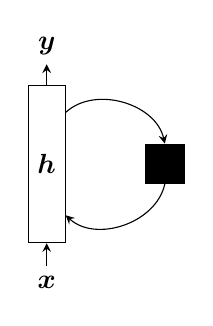
\begin{tikzpicture}[x=1.5cm, y=1.5cm]
        \node [] (input) at (0,0) {$\vect{x}$};
        
        \node [layer] (state) at (0,1) {$\vect{h}$};
        \node [delay] (delay) at (1,1) {};
        
        \node [] (output) at (0,2) {$\vect{y}$};
        
        \draw [arrow] (input) -- (state);
        \draw [arrow] (state) -- (output);
        \draw (state) edge[arrow, bend left=60] (delay.north);
        \draw (delay.south) edge[arrow, bend left=60] (state);
      \end{tikzpicture}
    }\hfill
    % \subfigure[]{
    \subfloat[\label{fig:rnn2}]{
      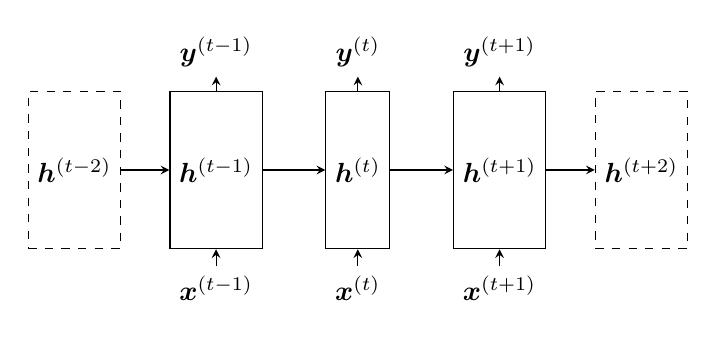
\begin{tikzpicture}[x=1.5cm, y=1.5cm]
        \foreach \l [count=\i] in {t-1,t,t+1}{
          \node [] (input-\i) at (\i*1.2,0) {$\vect{x}^{(\l)}$};
          \node [layer] (state-\i) at (\i*1.2,1) {$\vect{h}^{(\l)}$};
          \node [] (output-\i) at (\i*1.2,2) {$\vect{y}^{(\l)}$};
          
          \draw [arrow] (input-\i) -- (state-\i);
          \draw [arrow] (state-\i) -- (output-\i);
        }
        \node [layer, dashed] (state-l) at (0,1) {$\vect{h}^{(t-2)}$};
        \node [layer, dashed] (state-r) at (4*1.2,1) {$\vect{h}^{(t+2)}$};
        
        \draw [arrow] (state-l) -- (state-1);
        \draw [arrow] (state-1) -- (state-2);
        \draw [arrow] (state-2) -- (state-3);
        \draw [arrow] (state-3) -- (state-r);
      \end{tikzpicture}
    }
    \caption{\acs{rnn}, folded (a) and unfolded (b) models.}
    %\label{fig:rnn}
  \end{figure}
  \begin{equation*}
    \vect{h}^{(t)} = f(\vect{h}^{(t-1)}, \vect{x}^{(t)}; \vect{\theta})
  \end{equation*}
\end{frame}

\begin{frame}{\acf{lstm}}
  \vspace{-0.85cm}
  \begin{figure}
  \centering
  % \subfigure[]{
  \subfloat[]{
    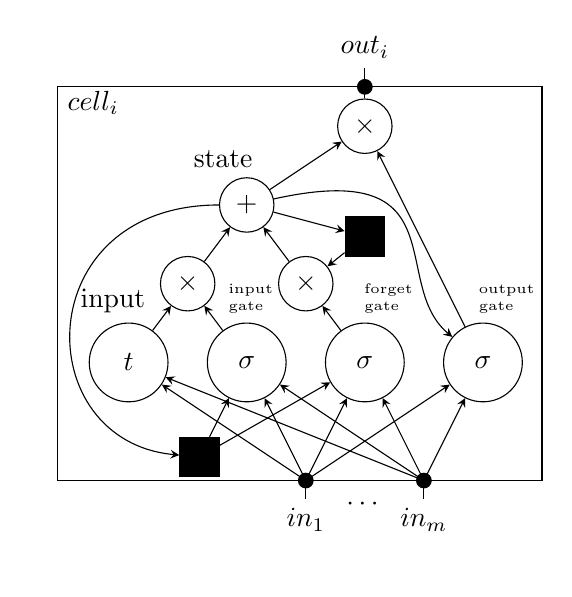
\begin{tikzpicture}[x=1.5cm, y=1cm]
      \node at (1,-0.5) {};

      \node[delay] (delay1) at (1.6,0.8) {};
      \coordinate (input1) at (2.5,0.5);
      \coordinate (input2) at (3.5,0.5);
      \node[] (input01) at (2.5,0) {$in_1$};
      \node[] (input02) at (3.5,0) {$in_m$};
      \node[] at (3,0.2) {$\cdots$};
      \node[every neuron, label={[xshift=-2mm]input}] (inputN) at (1,2) {$t$};
      \node[every neuron, label={[xshift=0.5mm, align=left, font=\tiny] input\\gate}] (inputGate) at (2,2) {$\sigma$};
      \node[every neuron, label={[xshift=3mm, align=left, font=\tiny] forget\\gate}] (forgetGate) at (3,2) {$\sigma$};
      \node[every neuron, label={[xshift=3mm, align=left, font=\tiny] output\\gate}] (outputGate) at (4,2) {$\sigma$};
      \node[operation] (inputTimes) at (1.5, 3) {$\times$};
      \node[operation, label={[xshift=-3mm]state}] (state) at (2, 4) {$+$};
      \node[delay] (delay2) at (3.0,3.6) {};
      \node[operation] (forgetTimes) at (2.5, 3) {$\times$};
      \node[operation] (outputTimes) at (3, 5) {$\times$};
      \coordinate (output1) at (3,5.5);
      \node (output2) at (3,6) {$out_i$};
      \node at (0.7,5.3) {$cell_i$};

      \fill[black] (input1) circle (1mm);
      \fill[black] (input2) circle (1mm);
      \fill[black] (output1) circle (1mm);
      
      \foreach \n in {input1, input2}{
        \foreach \m in {inputN, inputGate, forgetGate, outputGate}{
          \draw[arrow] (\n) -- (\m);
        }
      }
      \foreach \m in {inputGate, forgetGate}{
        \draw[arrow] (delay1) -- (\m);
      }

      \draw[arrow] (inputN) -- (inputTimes);
      \draw[arrow] (inputGate) -- (inputTimes);
      \draw[arrow] (forgetGate) -- (forgetTimes);
      \draw[arrow] (inputTimes) -- (state);
      \draw[arrow] (forgetTimes) -- (state);
      \draw [arrow] (state) ..  controls  (0.15,4) and (0.15,1) ..  (delay1);
      \draw [arrow] (state) ..  controls  (3.8,4.6) and (3.2,3) ..  (outputGate);
      \draw[arrow] (state) -- (delay2);
      \draw[arrow] (delay2) -- (forgetTimes);
      \draw[arrow] (state) -- (outputTimes);
      \draw[arrow] (outputGate) -- (outputTimes);
      \draw[line] (outputTimes) -- (output1);
      \draw[line] (output1) -- (output2);
      \draw[line] (input01) -- (input1);
      \draw[line] (input02) -- (input2);

      \path[border] (0.4,0.5) -- (4.5,0.5) -- (4.5,5.5) -- (0.4,5.5) -- (0.4,0.5); 
      

    \end{tikzpicture}
    \label{fig:lstm1}
  }\hfill
  % \subfigure[]{
  \subfloat[]{
    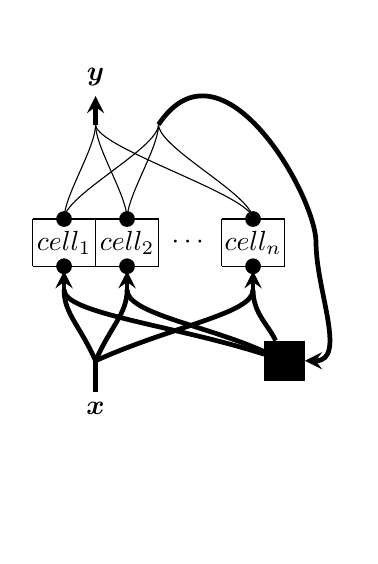
\begin{tikzpicture}[x=0.8cm, y=0.6cm]
      \node at (1,-2.5) {};

      % \draw[step=1.0,black,thin] (0,3) grid (4,4);
      \draw[step=1.0,black,thin] (0,3) grid (2,4);
      \draw[step=1.0,black,thin] (3,3) grid (4,4);
      \coordinate (input1) at (0.5,3);
      \coordinate (input2) at (1.5,3);
      \coordinate (input3) at (3.5,3);
      \coordinate (inputM1) at (0.5,2.5);
      \coordinate (inputM2) at (1.5,2.5);
      \coordinate (inputM3) at (3.5,2.5);
      \coordinate (output1) at (0.5,4);
      \coordinate (output2) at (1.5,4);
      \coordinate (output3) at (3.5,4);

      \coordinate (outputM) at (2,6);
      \coordinate (outputTM) at (1,6);
      
      \node at (0.5, 3.5) {$cell_1$};
      \node at (1.5, 3.5) {$cell_2$};
      \node at (2.5, 3.5) {$\cdots$};
      \node at (3.5, 3.5) {$cell_n$};
      \coordinate (pass) at (4.5, 3.5);
      \node (inputT) at (1,0) {$\vect{x}$};
      \coordinate (inputTM) at (1,1);
      \node (outputT) at (1,7) {$\vect{y}$};

      \node[delay] (delay) at (4,1) {};

      \foreach \c in {input1, input2, input3, output1, output2, output3}{
        \fill[black] (\c) circle (1mm);
      }

      \foreach \c in {inputM1, inputM2, inputM3}{
        \draw [vectorLine] (delay) ..  controls
        ($0.5*(delay)+0.5*(\c)$) and ($(\c)-(0,0.5)$) ..  (\c);
        \draw [vectorLine] (inputTM) ..  controls
        ($0.5*(inputTM)+0.5*(\c)$) and ($(\c)-(0,0.5)$) ..  (\c);
      }

      \foreach \c in {1, 2, 3}{
        \draw[vectorArrow] (inputM\c) -- ($(input\c)-(0,0.1)$);
      }

      \foreach \c in {output1, output2, output3}{
        \draw [line] (\c) ..  controls  ($(\c)+(0,0.5)$) and
        ($(outputM)-(0,0.5)$) ..  (outputM);
        \draw [line] (\c) ..  controls  ($(\c)+(0,0.5)$) and
        ($(outputTM)-(0,0.5)$) ..  (outputTM);
      }

      %\draw [vectorArrow] (outputM) ..  controls  ($(outputM)+(1,2)$) and ($(delay)+(1,0)$) ..  (delay);
      \draw [vectorArrow]
      (outputM) ..
      controls  ($(outputM)+(1,2)$) and ($(pass)+(0,1)$) ..
      (pass) ..
      controls  ($(pass)-(0,1)$) and ($(delay)+(1,0)$) ..
      (delay);
      \draw[vectorLine] (inputT) -- (inputTM);
      \draw[vectorArrow] (outputTM) -- (outputT);
    \end{tikzpicture}
    \label{fig:lstm2}
  }
  \caption{memory cell (a), and general
    scheme (b). The black box is a delay}
  %\label{fig:lstm}
\end{figure}
\end{frame}

\begin{frame}{\acf{gru}}
  \vspace{-0.8cm}
\begin{figure}
  \centering
  % \subfigure[]{
  \subfloat[]{
    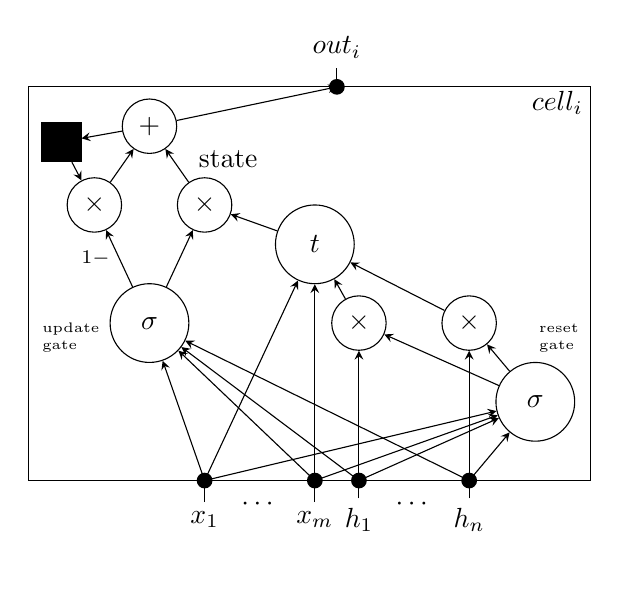
\begin{tikzpicture}[x=1.4cm, y=1cm]
      \node at (1,-0.5) {};

      \coordinate (input1) at (1,0.5);
      \coordinate (input2) at (2,0.5);
      \coordinate (input3) at (2.4,0.5);
      \coordinate (input4) at (3.4,0.5);
      \node[] (input01) at (1,0) {$x_1$};
      \node[] (input02) at (2,0) {$x_m$};
      \node[] (input03) at (2.4,0) {$h_1$};
      \node[] (input04) at (3.4,0) {$h_n$};
      \node[] at (1.5,0.2) {$\cdots$};
      \node[] at (2.9,0.2) {$\cdots$};
      \node[every neuron, label={[xshift=-10mm, yshift=-10mm, align=left, font=\tiny]update\\gate}] (updateGate) at (0.5,2.5) {$\sigma$};
      \node[every neuron, label={[xshift=3mm, align=left, font=\tiny] reset\\gate}] (resetGate) at (4,1.5) {$\sigma$};
      \node[operation] (updateTimesLeft) at (0, 4) {$\times$};
      \node[operation] (updateTimesRight) at (1, 4) {$\times$};
      \node[operation, label={[xshift=10mm,yshift=-10mm]state}] (state) at (0.5, 5) {$+$};
      \node[delay] (delay) at (-0.3,4.8) {};
      \node[operation] (resetTimesLeft) at (2.4, 2.5) {$\times$};
      \node[operation] (resetTimesRight) at (3.4, 2.5) {$\times$};
      \node[every neuron] (candidateState) at (2,3.5) {$t$};
      \coordinate (output1) at (2.2,5.5);
      \node (output2) at (2.2,6) {$out_i$};
      \node at (4.2,5.3) {$cell_i$};

      \fill[black] (input1) circle (1mm);
      \fill[black] (input2) circle (1mm);
      \fill[black] (input3) circle (1mm);
      \fill[black] (input4) circle (1mm);
      \fill[black] (output1) circle (1mm);
      
      \foreach \n in {input1, input2, input3, input4}{
        \foreach \m in {updateGate, resetGate}{
          \draw[arrow] (\n) -- (\m);
        }
      }

      \foreach \n in {input1, input2, resetTimesLeft, resetTimesRight}{
        \draw[arrow] (\n) -- (candidateState);
      }
      
      \draw[arrow] (updateGate) -- (updateTimesLeft) node[draw=none,fill=none,font=\scriptsize,midway,left] {$1-$};
      \draw[arrow] (updateGate) -- (updateTimesRight);
      \draw[arrow] (updateTimesLeft) -- (state);
      \draw[arrow] (updateTimesRight) -- (state);
      %\draw [arrow] (state) ..  controls  (3.8,4.2) and (3.2,3) ..  (resetGate);
      \draw[arrow] (state) -- (delay);
      \draw[arrow] (delay) -- (updateTimesLeft);
      \draw[arrow] (state) -- (output1);
      \draw[arrow] (input3) -- (resetTimesLeft);
      \draw[arrow] (input4) -- (resetTimesRight);
      \draw[arrow] (resetGate) -- (resetTimesLeft);
      \draw[arrow] (resetGate) -- (resetTimesRight);
      \draw[arrow] (candidateState) -- (updateTimesRight);
      \draw[line] (output1) -- (output2);
      \draw[line] (input01) -- (input1);
      \draw[line] (input02) -- (input2);
      \draw[line] (input03) -- (input3);
      \draw[line] (input04) -- (input4);

      \path[border] (-0.6,0.5) -- (4.5,0.5) -- (4.5,5.5) -- (-0.6,5.5) -- (-0.6,0.5); 
    \end{tikzpicture}
    %\label{fig:gru1}
  }\hfill
  % \subfigure[]{
  \subfloat[]{
    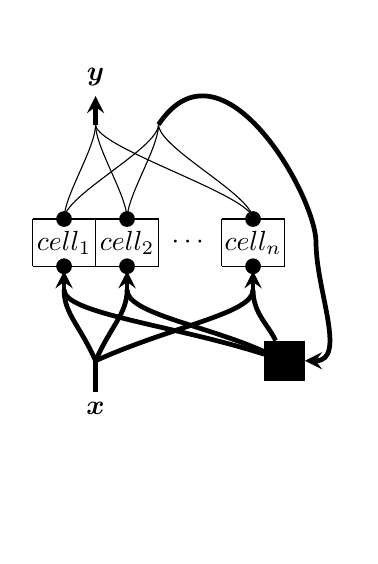
\begin{tikzpicture}[x=0.8cm, y=0.6cm]
      \node at (1,-2.5) {};

      % \draw[step=1.0,black,thin] (0,3) grid (4,4);
      \draw[step=1.0,black,thin] (0,3) grid (2,4);
      \draw[step=1.0,black,thin] (3,3) grid (4,4);
      \coordinate (input1) at (0.5,3);
      \coordinate (input2) at (1.5,3);
      \coordinate (input3) at (3.5,3);
      \coordinate (inputM1) at (0.5,2.5);
      \coordinate (inputM2) at (1.5,2.5);
      \coordinate (inputM3) at (3.5,2.5);
      \coordinate (output1) at (0.5,4);
      \coordinate (output2) at (1.5,4);
      \coordinate (output3) at (3.5,4);

      \coordinate (outputM) at (2,6);
      \coordinate (outputTM) at (1,6);
      
      \node at (0.5, 3.5) {$cell_1$};
      \node at (1.5, 3.5) {$cell_2$};
      \node at (2.5, 3.5) {$\cdots$};
      \node at (3.5, 3.5) {$cell_n$};
      \coordinate (pass) at (4.5, 3.5);
      \node (inputT) at (1,0) {$\vect{x}$};
      \coordinate (inputTM) at (1,1);
      \node (outputT) at (1,7) {$\vect{y}$};

      \node[delay] (delay) at (4,1) {};

      \foreach \c in {input1, input2, input3, output1, output2, output3}{
        \fill[black] (\c) circle (1mm);
      }

      \foreach \c in {inputM1, inputM2, inputM3}{
        \draw [vectorLine] (delay) ..  controls
        ($0.5*(delay)+0.5*(\c)$) and ($(\c)-(0,0.5)$) ..  (\c);
        \draw [vectorLine] (inputTM) ..  controls
        ($0.5*(inputTM)+0.5*(\c)$) and ($(\c)-(0,0.5)$) ..  (\c);
      }

      \foreach \c in {1, 2, 3}{
        \draw[vectorArrow] (inputM\c) -- ($(input\c)-(0,0.1)$);
      }

      \foreach \c in {output1, output2, output3}{
        \draw [line] (\c) ..  controls  ($(\c)+(0,0.5)$) and
        ($(outputM)-(0,0.5)$) ..  (outputM);
        \draw [line] (\c) ..  controls  ($(\c)+(0,0.5)$) and
        ($(outputTM)-(0,0.5)$) ..  (outputTM);
      }

      %\draw [vectorArrow] (outputM) ..  controls  ($(outputM)+(1,2)$) and ($(delay)+(1,0)$) ..  (delay);
      \draw [vectorArrow]
      (outputM) ..
      controls  ($(outputM)+(1,2)$) and ($(pass)+(0,1)$) ..
      (pass) ..
      controls  ($(pass)-(0,1)$) and ($(delay)+(1,0)$) ..
      (delay);
      \draw[vectorLine] (inputT) -- (inputTM);
      \draw[vectorArrow] (outputTM) -- (outputT);
    \end{tikzpicture}
    %\label{fig:gru2}
  }
  \caption{memory cell (a), and general
    scheme (b). The black box is a delay}
  %\label{fig:gru}
\end{figure}
\end{frame}

\begin{frame}{Word vectors}
  \begin{itemize}
  \item \alert{Transforms} words in vectors
  \item \alert{Unsupervised} learning method
  \item \alert{Semantic} relations encoded in vector space geometric relations 
  \end{itemize}
  \begin{center}
    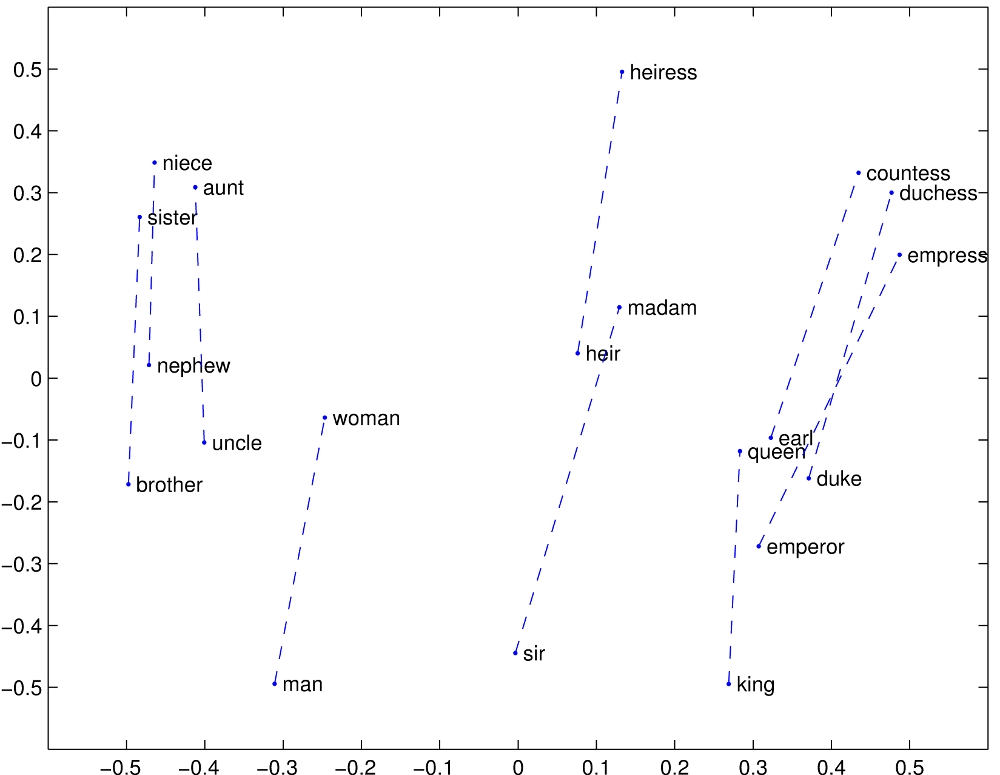
\includegraphics[width=0.6\textwidth]{img/man_woman.jpg}
  \end{center}
\end{frame}

\subsection{Attention Models}

\begin{frame}{Attention models}
  \begin{itemize}
  \item Developed for seq-to-seq task
  \item State of the art in machine translation
  \end{itemize}
  \begin{center}
    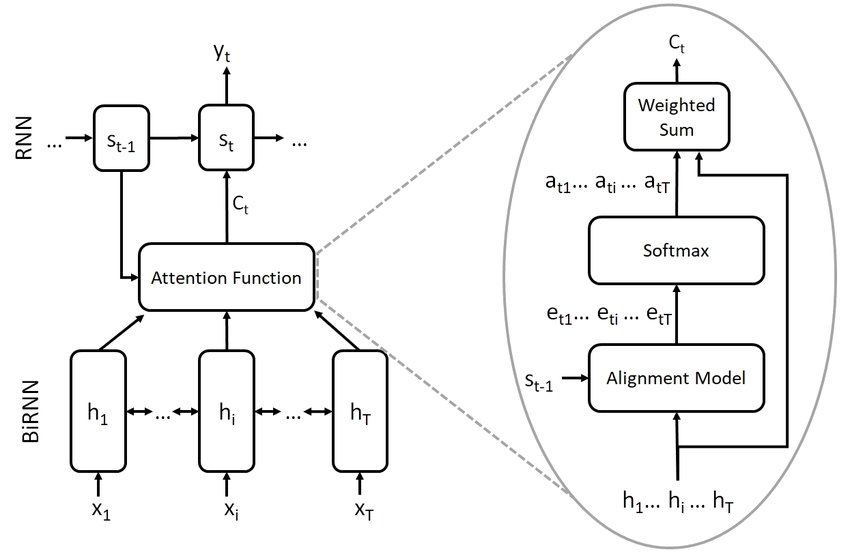
\includegraphics[width=0.6\textwidth]{img/attention.jpg}
  \end{center}  
\end{frame}

\subsection{Hierarchical models}
\begin{frame}{Hierarchical models}
  
\end{frame}

\subsection{\acs{bert}}
\begin{frame}{\acf{bert}}
  
\end{frame}

\section{Materials and Methods}

\subsection{Datasets}
\begin{frame}{Dataset}
  \begin{itemize}
  \item \alert{$1\,592\,385$} anatomopathological exam results
    \begin{itemize}
    \item From \alert{Tuscany} cancer registry
    \item In period \alert{2004-2013}
    \end{itemize}
  \item \alert{$94\,524$} ($6\%$) labeled
  \end{itemize}
  \begin{block}{Structure}
    \begin{itemize}
    \item 3 text \alert{fields}: macroscopy, diagnosis, anamnesis
    \item field \alert{length} from 0 to 1368 (quartiles 34, 62, 134)
    \end{itemize}
  \end{block}
\end{frame}

\begin{frame}{Preparation}
  \begin{itemize}
  \item Data comes in \alert{two} tables to merge:
    \begin{enumerate}
    \item neoplasm table, containing administrative and clinical variables
    \item histology table, containing the text fields
    \end{enumerate}
    \begin{itemize}
    \item there are neoplasms without histology associated
      \begin{itemize}
      \item (register have access to more data)
      \end{itemize}
    \item there are histologies without neoplasm associated
      \begin{itemize}
      \item (not tumor biopsies) 
      \end{itemize}
    \end{itemize}
  \item The 3 text fields are \alert{merged}
  \end{itemize}
\end{frame}

\begin{frame}
  \centering
  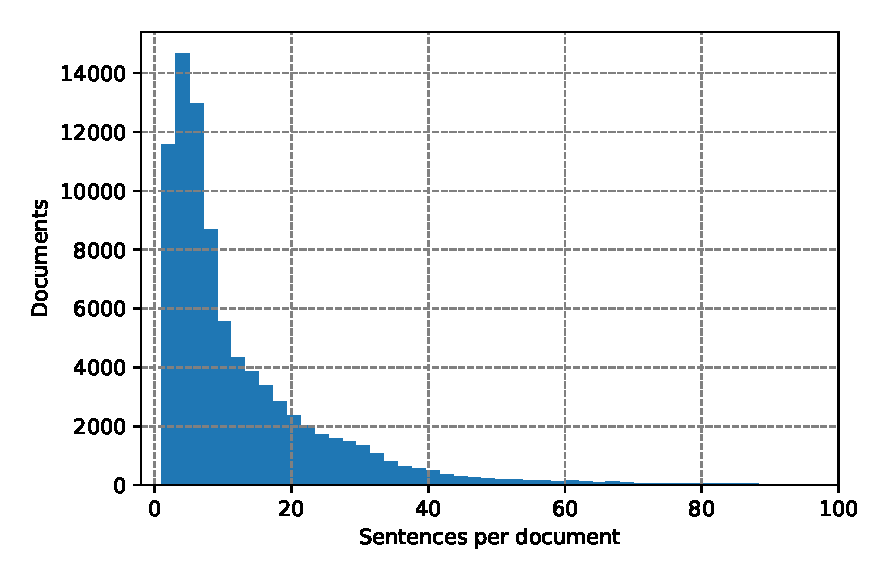
\includegraphics[width=0.6\textwidth]{img/sentPerDoc.eps}
  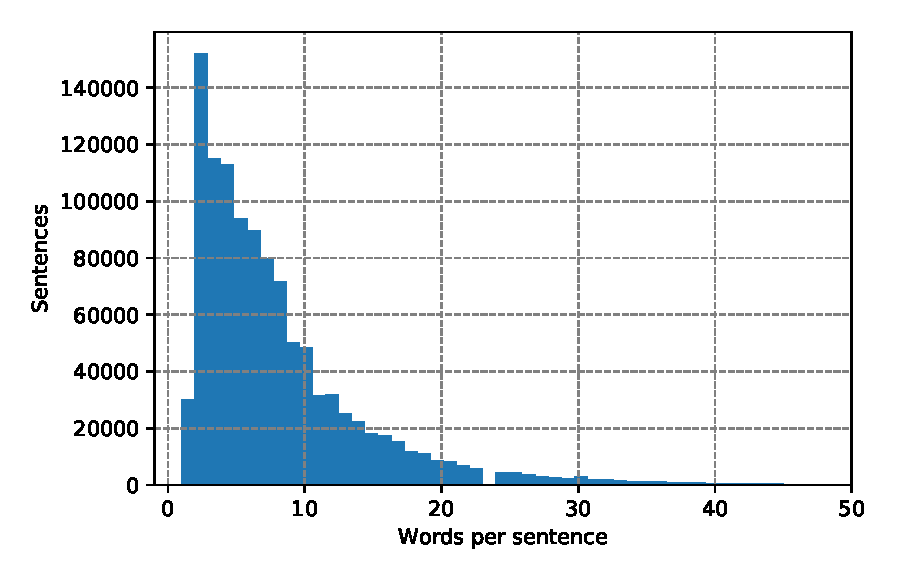
\includegraphics[width=0.6\textwidth]{img/wordPerSent.eps}
\end{frame}

\begin{frame}
  \centering
  \includegraphics[width=0.55\textwidth]{img/classDist-icdo3-site.pdf}
  \includegraphics[width=0.55\textwidth]{img/classDist-icdo3-type.pdf}
\end{frame}

\subsection{Models}
\begin{frame}{Models}
  \small
  \begin{description}
  \item[\svm] \alert{\acs{svm}} trained on \alert{\acs{tfidf}} representations using \alert{unigrams}
  \item[\svmb] \alert{\acs{svm}} trained on \alert{\acs{tfidf}} using
    \alert{unigrams} and \alert{bigrams}
  \item[\xgb] \alert{XGBoost} trained on \alert{\acs{tfidf}} using
    \alert{unigrams} and \alert{bigrams}
  \item[\lstmng] \alert{\acs{lstm}} trained on \alert{\acs{tfidf}} using
    \alert{bigrams}
  \item[\lstmc] mixed \alert{convolutional} and \alert{\ac{lstm}} trained on
    \alert{\acs{glove}}
  \item[\lstmb] \alert{\acs{lstm}} trained on \alert{\acs{glove}}
  \item[\gru] \alert{\acs{gru}} trained on \alert{\acs{glove}}
  \item[\maxp] \alert{\acs{gru}} with \alert{max} pooling trained on \alert{\acs{glove}}
  \item[\softmax] \alert{\acs{gru}} with \alert{attention} trained on \alert{\acs{glove}}
  \item[\maxi] \alert{\acs{gru}} with \alert{max} pooling, in \alert{interpretable} setting, trained on \alert{\acs{glove}}
  \item[\softmaxi] \alert{\acs{gru}} with \alert{attention}, in \alert{interpretable} setting, trained on \alert{\acs{glove}}
  \item[\maxh] \alert{hierarchical \acs{gru}} with \alert{max} pooling trained on \alert{\acs{glove}}
  \item[\softmaxh] \alert{hierarchical \acs{gru}} with \alert{attention} trained on \alert{\acs{glove}}
  \item[\bert] \alert{pretrained} on unlabeled data and \alert{fine tuned} with labeled data
  \end{description}
\end{frame}

\begin{frame}{\lstmng, \lstmc, \lstmb}
  \begin{figure}
  \centering
  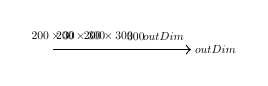
\begin{tikzpicture}[node distance = 0.1cm, auto]
    \begin{scope}[scale=0.7, transform shape]
    \begin{scope}[start chain, every node/.style={on chain}, node distance = \schemeNodeDistance]
      \nodeInput();
      \nodeEmbedding();
      \node[support] (emb) {};
      \nodeLstm();
      \node[support] (lstmA) {};
      \nodeLstm();
      \node[support] (lstmB) {};
      \nodeAvg();
      \node[support] (avg) {};
      \nodeRelu();
      \node[support] (relu) {};
      \nodeSoftmax();
      \node[dataLabel, joined] {$outDim$};
    \end{scope}
    \node[dataLabel, above=of emb] {$200\times 30$};
    \node[dataLabel, above=of lstmA] {$200\times 300$};
    \node[dataLabel, above=of lstmB] {$200\times 300$};
    \node[dataLabel, above=of avg] {$300$};
    \node[dataLabel, above=of relu] {$outDim$};
    \end{scope}
  \end{tikzpicture}
  \caption{Scheme for \lstmng{} model.}
\end{figure}

\begin{figure}
  \centering
  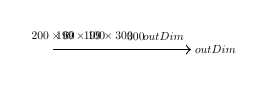
\begin{tikzpicture}[node distance = 0.1cm, auto]
    \begin{scope}[scale=0.7, transform shape]
      \begin{scope}[start chain, every node/.style={on chain}, node
      distance = \schemeNodeDistance]
      \nodeInput();
      \nodeGlove();
      \node[support] (glove) {};
      \nodeConv();
      \node[support] (conv) {};
      \nodeLstm();
      \node[support] (lstm) {};
      \nodeAvg();
      \node[support] (avg) {};
      \nodeRelu();
      \node[support] (relu) {};
      \nodeSoftmax();
      \node[dataLabel, joined] {$outDim$};
    \end{scope}
    \node[dataLabel, above=of glove] {$200\times 60$};
    \node[dataLabel, above=of conv] {$199\times 100$};
    \node[dataLabel, above=of lstm] {$199\times 300$};
    \node[dataLabel, above=of avg] {$300$};
    \node[dataLabel, above=of relu] {$outDim$};
  \end{scope}
  \end{tikzpicture}
  \caption{Scheme for \lstmc{} model.}
\end{figure}

\begin{figure}
  \centering
  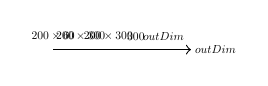
\begin{tikzpicture}[node distance = 0.1cm, auto]
    \begin{scope}[scale=0.7, transform shape]
    \begin{scope}[start chain, every node/.style={on chain}, node distance = \schemeNodeDistance]
      \nodeInput();
      \nodeGlove();
      \node[support] (glove) {};
      \nodeLstm();
      \node[support] (lstmA) {};
      \nodeLstm();
      \node[support] (lstmB) {};
      \nodeAvg();
      \node[support] (avg) {};
      \nodeRelu();
      \node[support] (relu) {};
      \nodeSoftmax();
      \node[dataLabel, joined] {$outDim$};
    \end{scope}
    \node[dataLabel, above=of glove] {$200\times 60$};
    \node[dataLabel, above=of lstmA] {$200\times 300$};
    \node[dataLabel, above=of lstmB] {$200\times 300$};
    \node[dataLabel, above=of avg] {$300$};
    \node[dataLabel, above=of relu] {$outDim$};
    \end{scope}
  \end{tikzpicture}
  \caption{Scheme for \lstmb{} model.}
\end{figure}
\end{frame}

\begin{frame}{\gru, \maxp, \softmax}
  \begin{block}{Plain model}
  \begin{align*}
  e_t &= E(x_t;\theta^e)\\
  h^f_t &= F(e_t,h^f_{t-1};\theta^f)\\
  h^r_t &= R(e_t,h^r_{t+1};\theta^r)\\
  u_t &= G(h_t;\theta^h)\\
  \phi &= A(\vect{u};\theta^a)\\
  f(\vect{x}) &= g(\phi;\theta^c)
  \end{align*}    
  \end{block}
  \begin{itemize}
  \item $\phi=(h^f_T,h^r_1)$ (in this case $G$ is the identity
    function)
  \item
    $\phi = \sum_t a_t(\vect{u};\theta^a) u_t$, $a_t(\vect{u};\theta^a) = \frac{e^{\langle c, c_t\rangle}}
    {\sum_i{e^{\langle c, c_i\rangle}}}$, $c_t=C(\vect{u};\theta^a)$
\item $\phi_j = \max_t u_{j,t}$
\end{itemize}
\end{frame}

\begin{frame}{\maxi, \softmaxi}
  \begin{block}{Interpretable model}
    \begin{align*}
  e_t &= E(x_t;\theta^e)\\
  h^f_t &= F(e_t,h^f_{t-1};\theta^f)\\
  h^r_t &= R(e_t,h^r_{t+1};\theta^r)\\
  u_t &= G(h_t;\theta^h)\\
  f(\vect{x}) &= A(\vect{u};\theta^a)
\end{align*}
  \end{block}
  \begin{itemize}
  \item
    $\phi = \sum_t a_t(\vect{u};\theta^a) u_t$, $a_t(\vect{u};\theta^a) = \frac{e^{\langle c, c_t\rangle}}
    {\sum_i{e^{\langle c, c_i\rangle}}}$, $c_t=C(\vect{u};\theta^a)$
\item $\phi_j = \max_t u_{j,t}$
\end{itemize}
\end{frame}

\begin{frame}{\maxh, \softmaxh}
  \begin{block}{Hierarchical model}
    \begin{align*}
  e_{s,t} &= E(x_{s,t};\theta^e)\\
  h^f_{s,t} &= F(e_{s,t},h^f_{s,t-1};\theta^{f})\\
  h^r_{s,t} &= R(e_{s,t},h^r_{s,t+1};\theta^{r})\\
  u_{s,t} &= G(h_{s,t};\theta^{h})\\
  \phi_s &= A(\vect{u}_s;\theta^{a})\\
  \bar{h}^{f}_{s} &= \bar{F}(\phi_{s},\bar{h}^{f}_{s-1};\bar{\theta}^{f})\\
  \bar{h}^{r}_{s} &= \bar{R}(\phi_{s},\bar{h}^{r}_{s+1};\bar{\theta}^{r})\\
  \bar{\phi} &= \bar{A}(\bar{\vect{h}};\bar{\theta}^{a})\\
  f(\vect{x}) &= g(\bar{\phi};\theta^c)
\end{align*}
  \end{block}
\end{frame}

\section{Experiments}



\subsection{Bag-of-words VS word vectors, \acs{svm} VS deep learning}

\begin{frame}{Bag-of-words VS word vectors, \acs{svm} VS deep learning}
  \begin{block}{Answered questions}
  \begin{itemize}
  \item[Q1] Implement \alert{large scale} study on deep learning
    applied to pathology reports
  \item[Q3] \alert{Compare} classical \alert{bag-of-words} techniques with
    newer deep learning techniques in this domain
  \item[Q5] \alert{Investigate} the contribution and applicability of
    \alert{unsupervised} learning techniques on uncommon text corpora
  \end{itemize}
\end{block}
\begin{itemize}
\item \alert{10-fold} cross validation
\item All tasks (\alert{main} site, \alert{subsite}, \alert{type},
  \alert{behavior})
\end{itemize}
\end{frame}

\begin{frame}{Bag-of-words VS word vectors, \acs{svm} VS deep learning}
\begin{table}
  \centering
  \caption{Results for \site{} task.}
  %\scriptsize
  \footnotesize
  %\small
          \begin{tabular}{|l|l|r@{$\;\pm\;$}l|r@{$\;\pm\;$}l|r@{$\;\pm\;$}l|r@{$\;\pm\;$}l|r@{$\;\pm\;$}l|}
            \hline
            \multicolumn{2}{|c|}{} & \multicolumn{2}{c|}{\svm} & \multicolumn{2}{c|}{\svmb} & \multicolumn{2}{c|}{\lstmng} & \multicolumn{2}{c|}{\lstmc} & \multicolumn{2}{c|}{\lstmb}\\
            \hline
            \multicolumn{2}{|l|}{\textbf{accuracy}} & $89.8$ & $2.0$ & $89.8$ & $2.0$ & $88.6$ & $2.0$ & $90.0$ & $1.6$ & \underline{$90.5$} & $1.6$ \\
            \hline
            \multicolumn{2}{|l|}{\textbf{kappa}} & $88.5$ & $2.2$ & $88.6$ & $2.3$ & $87.2$ & $2.3$ & $88.9$ & $1.8$ & \underline{$89.3$} & $1.8$ \\
            \hline
            \multicolumn{2}{|l|}{\textbf{MAPs}} & $93.0$ & $1.5$ & $93.0$ & $1.5$ & $92.2$ & $1.5$ & $93.5$ & $1.2$ & \underline{$93.8$} & $1.1$ \\
            \hline
            \multicolumn{2}{|l|}{\textbf{MAPc}} & $61.6$ & $3.9$ & $61.3$ & $4.0$ & $55.7$ & $3.7$ & $62.7$ & $3.5$ & \underline{$64.1$} & $4.1$ \\
            \hline
            \multirow{2}{*}{\textbf{pre.}} & \textbf{ma.} & \underline{$65.5$} & $4.8$ & $64.7$ & $3.2$ & $55.0$ & $2.8$ & $61.5$ & $3.4$ & $61.8$ & $3.7$ \\
            \cline{2-12}& \textbf{we.} & $88.7$ & $2.0$ & $88.8$ & $2.0$ & $87.8$ & $1.8$ & $89.2$ & $1.6$ & \underline{$89.5$} & $1.7$ \\
            \hline
            \multirow{2}{*}{\textbf{rec.}} & \textbf{ma.} & $55.7$ & $4.1$ & $54.7$ & $3.8$ & $51.6$ & $3.2$ & $56.5$ & $3.0$ & \underline{$58.1$} & $3.5$ \\
            \cline{2-12}& \textbf{we.} & $89.8$ & $2.0$ & $89.8$ & $2.0$ & $88.6$ & $2.0$ & $90.0$ & $1.6$ & \underline{$90.5$} & $1.6$ \\
            \hline
            \multirow{2}{*}{\textbf{f1s.}} & \textbf{ma.} & \underline{$58.4$} & $4.1$ & $57.5$ & $3.6$ & $52.1$ & $3.1$ & $57.0$ & $2.7$ & $58.2$ & $3.3$ \\
            \cline{2-12}& \textbf{we.} & $88.9$ & $2.0$ & $89.0$ & $2.1$ & $88.0$ & $2.0$ & $89.3$ & $1.6$ & \underline{$89.7$} & $1.7$ \\
            \hline
        \end{tabular}

\end{table}
\end{frame}

\begin{frame}{Bag-of-words VS word vectors, \acs{svm} VS deep learning}
\begin{figure}
  \centering
  \resizebox{0.9\textwidth}{!}{%% Creator: Matplotlib, PGF backend
%%
%% To include the figure in your LaTeX document, write
%%   \input{<filename>.pgf}
%%
%% Make sure the required packages are loaded in your preamble
%%   \usepackage{pgf}
%%
%% Figures using additional raster images can only be included by \input if
%% they are in the same directory as the main LaTeX file. For loading figures
%% from other directories you can use the `import` package
%%   \usepackage{import}
%% and then include the figures with
%%   \import{<path to file>}{<filename>.pgf}
%%
%% Matplotlib used the following preamble
%%   \newcommand{\svm}{xxxxxxxxxx}
%%   \newcommand{\svmb}{xxxxxxxxxx}
%%   \newcommand{\lstmng}{xxxxxxxxxx}
%%   \newcommand{\lstmc}{xxxxxxxxxx}
%%   \newcommand{\lstmb}{xxxxxxxxxx}
%%   \newcommand{\site}{xxxxxxxxxx}
%%   \newcommand{\fullSite}{xxxxxxxxxx}
%%   \newcommand{\type}{xxxxxxxxxx}
%%   \newcommand{\behaviour}{xxxxxxxxxx}
%%   \usepackage{fontspec}
%%
\begingroup%
\makeatletter%
\begin{pgfpicture}%
\pgfpathrectangle{\pgfpointorigin}{\pgfqpoint{5.392361in}{3.827777in}}%
\pgfusepath{use as bounding box, clip}%
\begin{pgfscope}%
\pgfsetbuttcap%
\pgfsetmiterjoin%
\definecolor{currentfill}{rgb}{1.000000,1.000000,1.000000}%
\pgfsetfillcolor{currentfill}%
\pgfsetlinewidth{0.000000pt}%
\definecolor{currentstroke}{rgb}{1.000000,1.000000,1.000000}%
\pgfsetstrokecolor{currentstroke}%
\pgfsetdash{}{0pt}%
\pgfpathmoveto{\pgfqpoint{0.000000in}{0.000000in}}%
\pgfpathlineto{\pgfqpoint{5.392361in}{0.000000in}}%
\pgfpathlineto{\pgfqpoint{5.392361in}{3.827777in}}%
\pgfpathlineto{\pgfqpoint{0.000000in}{3.827777in}}%
\pgfpathclose%
\pgfusepath{fill}%
\end{pgfscope}%
\begin{pgfscope}%
\pgfsetbuttcap%
\pgfsetmiterjoin%
\definecolor{currentfill}{rgb}{1.000000,1.000000,1.000000}%
\pgfsetfillcolor{currentfill}%
\pgfsetlinewidth{0.000000pt}%
\definecolor{currentstroke}{rgb}{0.000000,0.000000,0.000000}%
\pgfsetstrokecolor{currentstroke}%
\pgfsetstrokeopacity{0.000000}%
\pgfsetdash{}{0pt}%
\pgfpathmoveto{\pgfqpoint{0.553611in}{0.499444in}}%
\pgfpathlineto{\pgfqpoint{5.203611in}{0.499444in}}%
\pgfpathlineto{\pgfqpoint{5.203611in}{3.519444in}}%
\pgfpathlineto{\pgfqpoint{0.553611in}{3.519444in}}%
\pgfpathclose%
\pgfusepath{fill}%
\end{pgfscope}%
\begin{pgfscope}%
\pgfsetbuttcap%
\pgfsetroundjoin%
\definecolor{currentfill}{rgb}{0.000000,0.000000,0.000000}%
\pgfsetfillcolor{currentfill}%
\pgfsetlinewidth{0.803000pt}%
\definecolor{currentstroke}{rgb}{0.000000,0.000000,0.000000}%
\pgfsetstrokecolor{currentstroke}%
\pgfsetdash{}{0pt}%
\pgfsys@defobject{currentmarker}{\pgfqpoint{0.000000in}{-0.048611in}}{\pgfqpoint{0.000000in}{0.000000in}}{%
\pgfpathmoveto{\pgfqpoint{0.000000in}{0.000000in}}%
\pgfpathlineto{\pgfqpoint{0.000000in}{-0.048611in}}%
\pgfusepath{stroke,fill}%
}%
\begin{pgfscope}%
\pgfsys@transformshift{0.553611in}{0.499444in}%
\pgfsys@useobject{currentmarker}{}%
\end{pgfscope}%
\end{pgfscope}%
\begin{pgfscope}%
\pgftext[x=0.553611in,y=0.402222in,,top]{\sffamily\fontsize{10.000000}{12.000000}\selectfont 0.0}%
\end{pgfscope}%
\begin{pgfscope}%
\pgfsetbuttcap%
\pgfsetroundjoin%
\definecolor{currentfill}{rgb}{0.000000,0.000000,0.000000}%
\pgfsetfillcolor{currentfill}%
\pgfsetlinewidth{0.803000pt}%
\definecolor{currentstroke}{rgb}{0.000000,0.000000,0.000000}%
\pgfsetstrokecolor{currentstroke}%
\pgfsetdash{}{0pt}%
\pgfsys@defobject{currentmarker}{\pgfqpoint{0.000000in}{-0.048611in}}{\pgfqpoint{0.000000in}{0.000000in}}{%
\pgfpathmoveto{\pgfqpoint{0.000000in}{0.000000in}}%
\pgfpathlineto{\pgfqpoint{0.000000in}{-0.048611in}}%
\pgfusepath{stroke,fill}%
}%
\begin{pgfscope}%
\pgfsys@transformshift{1.483611in}{0.499444in}%
\pgfsys@useobject{currentmarker}{}%
\end{pgfscope}%
\end{pgfscope}%
\begin{pgfscope}%
\pgftext[x=1.483611in,y=0.402222in,,top]{\sffamily\fontsize{10.000000}{12.000000}\selectfont 0.2}%
\end{pgfscope}%
\begin{pgfscope}%
\pgfsetbuttcap%
\pgfsetroundjoin%
\definecolor{currentfill}{rgb}{0.000000,0.000000,0.000000}%
\pgfsetfillcolor{currentfill}%
\pgfsetlinewidth{0.803000pt}%
\definecolor{currentstroke}{rgb}{0.000000,0.000000,0.000000}%
\pgfsetstrokecolor{currentstroke}%
\pgfsetdash{}{0pt}%
\pgfsys@defobject{currentmarker}{\pgfqpoint{0.000000in}{-0.048611in}}{\pgfqpoint{0.000000in}{0.000000in}}{%
\pgfpathmoveto{\pgfqpoint{0.000000in}{0.000000in}}%
\pgfpathlineto{\pgfqpoint{0.000000in}{-0.048611in}}%
\pgfusepath{stroke,fill}%
}%
\begin{pgfscope}%
\pgfsys@transformshift{2.413611in}{0.499444in}%
\pgfsys@useobject{currentmarker}{}%
\end{pgfscope}%
\end{pgfscope}%
\begin{pgfscope}%
\pgftext[x=2.413611in,y=0.402222in,,top]{\sffamily\fontsize{10.000000}{12.000000}\selectfont 0.4}%
\end{pgfscope}%
\begin{pgfscope}%
\pgfsetbuttcap%
\pgfsetroundjoin%
\definecolor{currentfill}{rgb}{0.000000,0.000000,0.000000}%
\pgfsetfillcolor{currentfill}%
\pgfsetlinewidth{0.803000pt}%
\definecolor{currentstroke}{rgb}{0.000000,0.000000,0.000000}%
\pgfsetstrokecolor{currentstroke}%
\pgfsetdash{}{0pt}%
\pgfsys@defobject{currentmarker}{\pgfqpoint{0.000000in}{-0.048611in}}{\pgfqpoint{0.000000in}{0.000000in}}{%
\pgfpathmoveto{\pgfqpoint{0.000000in}{0.000000in}}%
\pgfpathlineto{\pgfqpoint{0.000000in}{-0.048611in}}%
\pgfusepath{stroke,fill}%
}%
\begin{pgfscope}%
\pgfsys@transformshift{3.343611in}{0.499444in}%
\pgfsys@useobject{currentmarker}{}%
\end{pgfscope}%
\end{pgfscope}%
\begin{pgfscope}%
\pgftext[x=3.343611in,y=0.402222in,,top]{\sffamily\fontsize{10.000000}{12.000000}\selectfont 0.6}%
\end{pgfscope}%
\begin{pgfscope}%
\pgfsetbuttcap%
\pgfsetroundjoin%
\definecolor{currentfill}{rgb}{0.000000,0.000000,0.000000}%
\pgfsetfillcolor{currentfill}%
\pgfsetlinewidth{0.803000pt}%
\definecolor{currentstroke}{rgb}{0.000000,0.000000,0.000000}%
\pgfsetstrokecolor{currentstroke}%
\pgfsetdash{}{0pt}%
\pgfsys@defobject{currentmarker}{\pgfqpoint{0.000000in}{-0.048611in}}{\pgfqpoint{0.000000in}{0.000000in}}{%
\pgfpathmoveto{\pgfqpoint{0.000000in}{0.000000in}}%
\pgfpathlineto{\pgfqpoint{0.000000in}{-0.048611in}}%
\pgfusepath{stroke,fill}%
}%
\begin{pgfscope}%
\pgfsys@transformshift{4.273611in}{0.499444in}%
\pgfsys@useobject{currentmarker}{}%
\end{pgfscope}%
\end{pgfscope}%
\begin{pgfscope}%
\pgftext[x=4.273611in,y=0.402222in,,top]{\sffamily\fontsize{10.000000}{12.000000}\selectfont 0.8}%
\end{pgfscope}%
\begin{pgfscope}%
\pgfsetbuttcap%
\pgfsetroundjoin%
\definecolor{currentfill}{rgb}{0.000000,0.000000,0.000000}%
\pgfsetfillcolor{currentfill}%
\pgfsetlinewidth{0.803000pt}%
\definecolor{currentstroke}{rgb}{0.000000,0.000000,0.000000}%
\pgfsetstrokecolor{currentstroke}%
\pgfsetdash{}{0pt}%
\pgfsys@defobject{currentmarker}{\pgfqpoint{0.000000in}{-0.048611in}}{\pgfqpoint{0.000000in}{0.000000in}}{%
\pgfpathmoveto{\pgfqpoint{0.000000in}{0.000000in}}%
\pgfpathlineto{\pgfqpoint{0.000000in}{-0.048611in}}%
\pgfusepath{stroke,fill}%
}%
\begin{pgfscope}%
\pgfsys@transformshift{5.203611in}{0.499444in}%
\pgfsys@useobject{currentmarker}{}%
\end{pgfscope}%
\end{pgfscope}%
\begin{pgfscope}%
\pgftext[x=5.203611in,y=0.402222in,,top]{\sffamily\fontsize{10.000000}{12.000000}\selectfont 1.0}%
\end{pgfscope}%
\begin{pgfscope}%
\pgftext[x=2.878611in,y=0.223333in,,top]{\sffamily\fontsize{10.000000}{12.000000}\selectfont Recall}%
\end{pgfscope}%
\begin{pgfscope}%
\pgfsetbuttcap%
\pgfsetroundjoin%
\definecolor{currentfill}{rgb}{0.000000,0.000000,0.000000}%
\pgfsetfillcolor{currentfill}%
\pgfsetlinewidth{0.803000pt}%
\definecolor{currentstroke}{rgb}{0.000000,0.000000,0.000000}%
\pgfsetstrokecolor{currentstroke}%
\pgfsetdash{}{0pt}%
\pgfsys@defobject{currentmarker}{\pgfqpoint{-0.048611in}{0.000000in}}{\pgfqpoint{0.000000in}{0.000000in}}{%
\pgfpathmoveto{\pgfqpoint{0.000000in}{0.000000in}}%
\pgfpathlineto{\pgfqpoint{-0.048611in}{0.000000in}}%
\pgfusepath{stroke,fill}%
}%
\begin{pgfscope}%
\pgfsys@transformshift{0.553611in}{0.499444in}%
\pgfsys@useobject{currentmarker}{}%
\end{pgfscope}%
\end{pgfscope}%
\begin{pgfscope}%
\pgftext[x=0.278889in,y=0.451250in,left,base]{\sffamily\fontsize{10.000000}{12.000000}\selectfont 0.0}%
\end{pgfscope}%
\begin{pgfscope}%
\pgfsetbuttcap%
\pgfsetroundjoin%
\definecolor{currentfill}{rgb}{0.000000,0.000000,0.000000}%
\pgfsetfillcolor{currentfill}%
\pgfsetlinewidth{0.803000pt}%
\definecolor{currentstroke}{rgb}{0.000000,0.000000,0.000000}%
\pgfsetstrokecolor{currentstroke}%
\pgfsetdash{}{0pt}%
\pgfsys@defobject{currentmarker}{\pgfqpoint{-0.048611in}{0.000000in}}{\pgfqpoint{0.000000in}{0.000000in}}{%
\pgfpathmoveto{\pgfqpoint{0.000000in}{0.000000in}}%
\pgfpathlineto{\pgfqpoint{-0.048611in}{0.000000in}}%
\pgfusepath{stroke,fill}%
}%
\begin{pgfscope}%
\pgfsys@transformshift{0.553611in}{1.074682in}%
\pgfsys@useobject{currentmarker}{}%
\end{pgfscope}%
\end{pgfscope}%
\begin{pgfscope}%
\pgftext[x=0.278889in,y=1.026488in,left,base]{\sffamily\fontsize{10.000000}{12.000000}\selectfont 0.2}%
\end{pgfscope}%
\begin{pgfscope}%
\pgfsetbuttcap%
\pgfsetroundjoin%
\definecolor{currentfill}{rgb}{0.000000,0.000000,0.000000}%
\pgfsetfillcolor{currentfill}%
\pgfsetlinewidth{0.803000pt}%
\definecolor{currentstroke}{rgb}{0.000000,0.000000,0.000000}%
\pgfsetstrokecolor{currentstroke}%
\pgfsetdash{}{0pt}%
\pgfsys@defobject{currentmarker}{\pgfqpoint{-0.048611in}{0.000000in}}{\pgfqpoint{0.000000in}{0.000000in}}{%
\pgfpathmoveto{\pgfqpoint{0.000000in}{0.000000in}}%
\pgfpathlineto{\pgfqpoint{-0.048611in}{0.000000in}}%
\pgfusepath{stroke,fill}%
}%
\begin{pgfscope}%
\pgfsys@transformshift{0.553611in}{1.649920in}%
\pgfsys@useobject{currentmarker}{}%
\end{pgfscope}%
\end{pgfscope}%
\begin{pgfscope}%
\pgftext[x=0.278889in,y=1.601726in,left,base]{\sffamily\fontsize{10.000000}{12.000000}\selectfont 0.4}%
\end{pgfscope}%
\begin{pgfscope}%
\pgfsetbuttcap%
\pgfsetroundjoin%
\definecolor{currentfill}{rgb}{0.000000,0.000000,0.000000}%
\pgfsetfillcolor{currentfill}%
\pgfsetlinewidth{0.803000pt}%
\definecolor{currentstroke}{rgb}{0.000000,0.000000,0.000000}%
\pgfsetstrokecolor{currentstroke}%
\pgfsetdash{}{0pt}%
\pgfsys@defobject{currentmarker}{\pgfqpoint{-0.048611in}{0.000000in}}{\pgfqpoint{0.000000in}{0.000000in}}{%
\pgfpathmoveto{\pgfqpoint{0.000000in}{0.000000in}}%
\pgfpathlineto{\pgfqpoint{-0.048611in}{0.000000in}}%
\pgfusepath{stroke,fill}%
}%
\begin{pgfscope}%
\pgfsys@transformshift{0.553611in}{2.225158in}%
\pgfsys@useobject{currentmarker}{}%
\end{pgfscope}%
\end{pgfscope}%
\begin{pgfscope}%
\pgftext[x=0.278889in,y=2.176964in,left,base]{\sffamily\fontsize{10.000000}{12.000000}\selectfont 0.6}%
\end{pgfscope}%
\begin{pgfscope}%
\pgfsetbuttcap%
\pgfsetroundjoin%
\definecolor{currentfill}{rgb}{0.000000,0.000000,0.000000}%
\pgfsetfillcolor{currentfill}%
\pgfsetlinewidth{0.803000pt}%
\definecolor{currentstroke}{rgb}{0.000000,0.000000,0.000000}%
\pgfsetstrokecolor{currentstroke}%
\pgfsetdash{}{0pt}%
\pgfsys@defobject{currentmarker}{\pgfqpoint{-0.048611in}{0.000000in}}{\pgfqpoint{0.000000in}{0.000000in}}{%
\pgfpathmoveto{\pgfqpoint{0.000000in}{0.000000in}}%
\pgfpathlineto{\pgfqpoint{-0.048611in}{0.000000in}}%
\pgfusepath{stroke,fill}%
}%
\begin{pgfscope}%
\pgfsys@transformshift{0.553611in}{2.800397in}%
\pgfsys@useobject{currentmarker}{}%
\end{pgfscope}%
\end{pgfscope}%
\begin{pgfscope}%
\pgftext[x=0.278889in,y=2.752202in,left,base]{\sffamily\fontsize{10.000000}{12.000000}\selectfont 0.8}%
\end{pgfscope}%
\begin{pgfscope}%
\pgfsetbuttcap%
\pgfsetroundjoin%
\definecolor{currentfill}{rgb}{0.000000,0.000000,0.000000}%
\pgfsetfillcolor{currentfill}%
\pgfsetlinewidth{0.803000pt}%
\definecolor{currentstroke}{rgb}{0.000000,0.000000,0.000000}%
\pgfsetstrokecolor{currentstroke}%
\pgfsetdash{}{0pt}%
\pgfsys@defobject{currentmarker}{\pgfqpoint{-0.048611in}{0.000000in}}{\pgfqpoint{0.000000in}{0.000000in}}{%
\pgfpathmoveto{\pgfqpoint{0.000000in}{0.000000in}}%
\pgfpathlineto{\pgfqpoint{-0.048611in}{0.000000in}}%
\pgfusepath{stroke,fill}%
}%
\begin{pgfscope}%
\pgfsys@transformshift{0.553611in}{3.375635in}%
\pgfsys@useobject{currentmarker}{}%
\end{pgfscope}%
\end{pgfscope}%
\begin{pgfscope}%
\pgftext[x=0.278889in,y=3.327440in,left,base]{\sffamily\fontsize{10.000000}{12.000000}\selectfont 1.0}%
\end{pgfscope}%
\begin{pgfscope}%
\pgftext[x=0.223333in,y=2.009444in,,bottom,rotate=90.000000]{\sffamily\fontsize{10.000000}{12.000000}\selectfont Precision}%
\end{pgfscope}%
\begin{pgfscope}%
\pgfpathrectangle{\pgfqpoint{0.553611in}{0.499444in}}{\pgfqpoint{4.650000in}{3.020000in}} %
\pgfusepath{clip}%
\pgfsetrectcap%
\pgfsetroundjoin%
\pgfsetlinewidth{1.505625pt}%
\definecolor{currentstroke}{rgb}{0.000000,0.000000,0.000000}%
\pgfsetstrokecolor{currentstroke}%
\pgfsetdash{}{0pt}%
\pgfpathmoveto{\pgfqpoint{0.553611in}{2.645855in}}%
\pgfpathlineto{\pgfqpoint{0.560440in}{2.662201in}}%
\pgfpathlineto{\pgfqpoint{0.562575in}{2.662837in}}%
\pgfpathlineto{\pgfqpoint{0.564473in}{2.679936in}}%
\pgfpathlineto{\pgfqpoint{0.565283in}{2.680450in}}%
\pgfpathlineto{\pgfqpoint{0.565294in}{2.673303in}}%
\pgfpathlineto{\pgfqpoint{0.566809in}{2.674938in}}%
\pgfpathlineto{\pgfqpoint{0.569669in}{2.679946in}}%
\pgfpathlineto{\pgfqpoint{0.574526in}{2.700887in}}%
\pgfpathlineto{\pgfqpoint{0.575914in}{2.707983in}}%
\pgfpathlineto{\pgfqpoint{0.576234in}{2.707392in}}%
\pgfpathlineto{\pgfqpoint{0.583781in}{2.723278in}}%
\pgfpathlineto{\pgfqpoint{0.585111in}{2.724468in}}%
\pgfpathlineto{\pgfqpoint{0.586544in}{2.732217in}}%
\pgfpathlineto{\pgfqpoint{0.588530in}{2.734492in}}%
\pgfpathlineto{\pgfqpoint{0.589670in}{2.743535in}}%
\pgfpathlineto{\pgfqpoint{0.590087in}{2.740476in}}%
\pgfpathlineto{\pgfqpoint{0.596260in}{2.747300in}}%
\pgfpathlineto{\pgfqpoint{0.596272in}{2.736903in}}%
\pgfpathlineto{\pgfqpoint{0.597799in}{2.740640in}}%
\pgfpathlineto{\pgfqpoint{0.602806in}{2.740021in}}%
\pgfpathlineto{\pgfqpoint{0.603636in}{2.739949in}}%
\pgfpathlineto{\pgfqpoint{0.604261in}{2.746997in}}%
\pgfpathlineto{\pgfqpoint{0.605303in}{2.745372in}}%
\pgfpathlineto{\pgfqpoint{0.611661in}{2.756726in}}%
\pgfpathlineto{\pgfqpoint{0.613264in}{2.764680in}}%
\pgfpathlineto{\pgfqpoint{0.614719in}{2.765891in}}%
\pgfpathlineto{\pgfqpoint{0.615076in}{2.744398in}}%
\pgfpathlineto{\pgfqpoint{0.616177in}{2.745172in}}%
\pgfpathlineto{\pgfqpoint{0.617210in}{2.745794in}}%
\pgfpathlineto{\pgfqpoint{0.618851in}{2.760914in}}%
\pgfpathlineto{\pgfqpoint{0.624062in}{2.765510in}}%
\pgfpathlineto{\pgfqpoint{0.624066in}{2.744049in}}%
\pgfpathlineto{\pgfqpoint{0.625587in}{2.745657in}}%
\pgfpathlineto{\pgfqpoint{0.625747in}{2.745819in}}%
\pgfpathlineto{\pgfqpoint{0.625747in}{2.745819in}}%
\pgfpathlineto{\pgfqpoint{0.625747in}{2.745819in}}%
\pgfpathlineto{\pgfqpoint{0.625844in}{2.744877in}}%
\pgfpathlineto{\pgfqpoint{0.626991in}{2.745941in}}%
\pgfpathlineto{\pgfqpoint{0.626991in}{2.745941in}}%
\pgfpathlineto{\pgfqpoint{0.627189in}{2.746123in}}%
\pgfpathlineto{\pgfqpoint{0.627189in}{2.746123in}}%
\pgfpathlineto{\pgfqpoint{0.627189in}{2.746123in}}%
\pgfpathlineto{\pgfqpoint{0.627208in}{2.745474in}}%
\pgfpathlineto{\pgfqpoint{0.627397in}{2.745651in}}%
\pgfpathlineto{\pgfqpoint{0.627397in}{2.745651in}}%
\pgfpathlineto{\pgfqpoint{0.628856in}{2.753724in}}%
\pgfpathlineto{\pgfqpoint{0.631370in}{2.754642in}}%
\pgfpathlineto{\pgfqpoint{0.632914in}{2.763887in}}%
\pgfpathlineto{\pgfqpoint{0.635601in}{2.765210in}}%
\pgfpathlineto{\pgfqpoint{0.635991in}{2.763134in}}%
\pgfpathlineto{\pgfqpoint{0.637082in}{2.763535in}}%
\pgfpathlineto{\pgfqpoint{0.638125in}{2.763781in}}%
\pgfpathlineto{\pgfqpoint{0.638156in}{2.770943in}}%
\pgfpathlineto{\pgfqpoint{0.639695in}{2.770831in}}%
\pgfpathlineto{\pgfqpoint{0.641154in}{2.765231in}}%
\pgfpathlineto{\pgfqpoint{0.644955in}{2.763050in}}%
\pgfpathlineto{\pgfqpoint{0.647314in}{2.761658in}}%
\pgfpathlineto{\pgfqpoint{0.647723in}{2.767425in}}%
\pgfpathlineto{\pgfqpoint{0.648866in}{2.766557in}}%
\pgfpathlineto{\pgfqpoint{0.650742in}{2.765705in}}%
\pgfpathlineto{\pgfqpoint{0.652410in}{2.770841in}}%
\pgfpathlineto{\pgfqpoint{0.658454in}{2.769812in}}%
\pgfpathlineto{\pgfqpoint{0.659027in}{2.774114in}}%
\pgfpathlineto{\pgfqpoint{0.659984in}{2.774063in}}%
\pgfpathlineto{\pgfqpoint{0.670335in}{2.773627in}}%
\pgfpathlineto{\pgfqpoint{0.670960in}{2.777514in}}%
\pgfpathlineto{\pgfqpoint{0.671831in}{2.777441in}}%
\pgfpathlineto{\pgfqpoint{0.678464in}{2.778609in}}%
\pgfpathlineto{\pgfqpoint{0.680965in}{2.780013in}}%
\pgfpathlineto{\pgfqpoint{0.681593in}{2.770246in}}%
\pgfpathlineto{\pgfqpoint{0.682517in}{2.770535in}}%
\pgfpathlineto{\pgfqpoint{0.690345in}{2.772315in}}%
\pgfpathlineto{\pgfqpoint{0.690376in}{2.768754in}}%
\pgfpathlineto{\pgfqpoint{0.691907in}{2.769436in}}%
\pgfpathlineto{\pgfqpoint{0.698077in}{2.771610in}}%
\pgfpathlineto{\pgfqpoint{0.698158in}{2.769031in}}%
\pgfpathlineto{\pgfqpoint{0.699599in}{2.770769in}}%
\pgfpathlineto{\pgfqpoint{0.700608in}{2.771102in}}%
\pgfpathlineto{\pgfqpoint{0.701230in}{2.759151in}}%
\pgfpathlineto{\pgfqpoint{0.702151in}{2.759208in}}%
\pgfpathlineto{\pgfqpoint{0.708554in}{2.761114in}}%
\pgfpathlineto{\pgfqpoint{0.708611in}{2.755428in}}%
\pgfpathlineto{\pgfqpoint{0.710062in}{2.756386in}}%
\pgfpathlineto{\pgfqpoint{0.716664in}{2.758900in}}%
\pgfpathlineto{\pgfqpoint{0.719652in}{2.759403in}}%
\pgfpathlineto{\pgfqpoint{0.719682in}{2.752254in}}%
\pgfpathlineto{\pgfqpoint{0.721194in}{2.753769in}}%
\pgfpathlineto{\pgfqpoint{0.723599in}{2.756192in}}%
\pgfpathlineto{\pgfqpoint{0.725779in}{2.757695in}}%
\pgfpathlineto{\pgfqpoint{0.725833in}{2.755337in}}%
\pgfpathlineto{\pgfqpoint{0.727335in}{2.756080in}}%
\pgfpathlineto{\pgfqpoint{0.729042in}{2.756904in}}%
\pgfpathlineto{\pgfqpoint{0.730573in}{2.761524in}}%
\pgfpathlineto{\pgfqpoint{0.732449in}{2.762387in}}%
\pgfpathlineto{\pgfqpoint{0.733980in}{2.770471in}}%
\pgfpathlineto{\pgfqpoint{0.737541in}{2.771284in}}%
\pgfpathlineto{\pgfqpoint{0.738473in}{2.766508in}}%
\pgfpathlineto{\pgfqpoint{0.739119in}{2.766844in}}%
\pgfpathlineto{\pgfqpoint{0.755891in}{2.777293in}}%
\pgfpathlineto{\pgfqpoint{0.766858in}{2.784123in}}%
\pgfpathlineto{\pgfqpoint{0.766914in}{2.782071in}}%
\pgfpathlineto{\pgfqpoint{0.768345in}{2.782784in}}%
\pgfpathlineto{\pgfqpoint{0.768739in}{2.782913in}}%
\pgfpathlineto{\pgfqpoint{0.770250in}{2.788730in}}%
\pgfpathlineto{\pgfqpoint{0.770446in}{2.788638in}}%
\pgfpathlineto{\pgfqpoint{0.778590in}{2.793160in}}%
\pgfpathlineto{\pgfqpoint{0.778611in}{2.782437in}}%
\pgfpathlineto{\pgfqpoint{0.780057in}{2.783106in}}%
\pgfpathlineto{\pgfqpoint{0.781712in}{2.783685in}}%
\pgfpathlineto{\pgfqpoint{0.781724in}{2.781034in}}%
\pgfpathlineto{\pgfqpoint{0.783251in}{2.781257in}}%
\pgfpathlineto{\pgfqpoint{0.793367in}{2.785378in}}%
\pgfpathlineto{\pgfqpoint{0.802406in}{2.789134in}}%
\pgfpathlineto{\pgfqpoint{0.802440in}{2.786615in}}%
\pgfpathlineto{\pgfqpoint{0.803943in}{2.787118in}}%
\pgfpathlineto{\pgfqpoint{0.804450in}{2.787282in}}%
\pgfpathlineto{\pgfqpoint{0.805179in}{2.776926in}}%
\pgfpathlineto{\pgfqpoint{0.806301in}{2.777349in}}%
\pgfpathlineto{\pgfqpoint{0.807154in}{2.773300in}}%
\pgfpathlineto{\pgfqpoint{0.808329in}{2.774801in}}%
\pgfpathlineto{\pgfqpoint{0.808405in}{2.762144in}}%
\pgfpathlineto{\pgfqpoint{0.809779in}{2.762323in}}%
\pgfpathlineto{\pgfqpoint{0.811870in}{2.762431in}}%
\pgfpathlineto{\pgfqpoint{0.811944in}{2.760708in}}%
\pgfpathlineto{\pgfqpoint{0.813331in}{2.761135in}}%
\pgfpathlineto{\pgfqpoint{0.821868in}{2.764283in}}%
\pgfpathlineto{\pgfqpoint{0.821880in}{2.761988in}}%
\pgfpathlineto{\pgfqpoint{0.823414in}{2.762698in}}%
\pgfpathlineto{\pgfqpoint{0.825958in}{2.762616in}}%
\pgfpathlineto{\pgfqpoint{0.827140in}{2.757980in}}%
\pgfpathlineto{\pgfqpoint{0.827496in}{2.758147in}}%
\pgfpathlineto{\pgfqpoint{0.836350in}{2.762640in}}%
\pgfpathlineto{\pgfqpoint{0.836381in}{2.758359in}}%
\pgfpathlineto{\pgfqpoint{0.837918in}{2.758890in}}%
\pgfpathlineto{\pgfqpoint{0.840235in}{2.759457in}}%
\pgfpathlineto{\pgfqpoint{0.840255in}{2.755502in}}%
\pgfpathlineto{\pgfqpoint{0.841728in}{2.756057in}}%
\pgfpathlineto{\pgfqpoint{0.848842in}{2.757162in}}%
\pgfpathlineto{\pgfqpoint{0.850370in}{2.760850in}}%
\pgfpathlineto{\pgfqpoint{0.853583in}{2.761371in}}%
\pgfpathlineto{\pgfqpoint{0.855043in}{2.767962in}}%
\pgfpathlineto{\pgfqpoint{0.863555in}{2.770550in}}%
\pgfpathlineto{\pgfqpoint{0.863611in}{2.759842in}}%
\pgfpathlineto{\pgfqpoint{0.865090in}{2.761583in}}%
\pgfpathlineto{\pgfqpoint{0.868237in}{2.762829in}}%
\pgfpathlineto{\pgfqpoint{0.868273in}{2.758246in}}%
\pgfpathlineto{\pgfqpoint{0.869808in}{2.758667in}}%
\pgfpathlineto{\pgfqpoint{0.872310in}{2.759654in}}%
\pgfpathlineto{\pgfqpoint{0.872361in}{2.757753in}}%
\pgfpathlineto{\pgfqpoint{0.873769in}{2.758295in}}%
\pgfpathlineto{\pgfqpoint{0.875436in}{2.757287in}}%
\pgfpathlineto{\pgfqpoint{0.875449in}{2.757237in}}%
\pgfpathlineto{\pgfqpoint{0.875712in}{2.757339in}}%
\pgfpathlineto{\pgfqpoint{0.875712in}{2.757339in}}%
\pgfpathlineto{\pgfqpoint{0.885693in}{2.761189in}}%
\pgfpathlineto{\pgfqpoint{0.885754in}{2.758139in}}%
\pgfpathlineto{\pgfqpoint{0.887282in}{2.758516in}}%
\pgfpathlineto{\pgfqpoint{0.897976in}{2.759637in}}%
\pgfpathlineto{\pgfqpoint{0.899219in}{2.756507in}}%
\pgfpathlineto{\pgfqpoint{0.900131in}{2.756734in}}%
\pgfpathlineto{\pgfqpoint{0.911866in}{2.758075in}}%
\pgfpathlineto{\pgfqpoint{0.923255in}{2.758501in}}%
\pgfpathlineto{\pgfqpoint{0.923276in}{2.756912in}}%
\pgfpathlineto{\pgfqpoint{0.924697in}{2.757263in}}%
\pgfpathlineto{\pgfqpoint{0.924697in}{2.757263in}}%
\pgfpathlineto{\pgfqpoint{0.926243in}{2.759784in}}%
\pgfpathlineto{\pgfqpoint{0.930554in}{2.760875in}}%
\pgfpathlineto{\pgfqpoint{0.930638in}{2.749836in}}%
\pgfpathlineto{\pgfqpoint{0.932173in}{2.750137in}}%
\pgfpathlineto{\pgfqpoint{0.935633in}{2.750715in}}%
\pgfpathlineto{\pgfqpoint{0.937342in}{2.752901in}}%
\pgfpathlineto{\pgfqpoint{0.948052in}{2.756306in}}%
\pgfpathlineto{\pgfqpoint{0.951724in}{2.757431in}}%
\pgfpathlineto{\pgfqpoint{0.951776in}{2.755097in}}%
\pgfpathlineto{\pgfqpoint{0.953297in}{2.755552in}}%
\pgfpathlineto{\pgfqpoint{0.962146in}{2.757160in}}%
\pgfpathlineto{\pgfqpoint{0.962188in}{2.755139in}}%
\pgfpathlineto{\pgfqpoint{0.963720in}{2.755577in}}%
\pgfpathlineto{\pgfqpoint{0.963813in}{2.755604in}}%
\pgfpathlineto{\pgfqpoint{0.963905in}{2.751542in}}%
\pgfpathlineto{\pgfqpoint{0.965360in}{2.751940in}}%
\pgfpathlineto{\pgfqpoint{0.981812in}{2.755923in}}%
\pgfpathlineto{\pgfqpoint{0.981900in}{2.748440in}}%
\pgfpathlineto{\pgfqpoint{0.983439in}{2.748622in}}%
\pgfpathlineto{\pgfqpoint{0.993411in}{2.749714in}}%
\pgfpathlineto{\pgfqpoint{0.994964in}{2.751646in}}%
\pgfpathlineto{\pgfqpoint{0.999456in}{2.751827in}}%
\pgfpathlineto{\pgfqpoint{1.000983in}{2.744894in}}%
\pgfpathlineto{\pgfqpoint{1.003569in}{2.745021in}}%
\pgfpathlineto{\pgfqpoint{1.004401in}{2.736836in}}%
\pgfpathlineto{\pgfqpoint{1.005085in}{2.737202in}}%
\pgfpathlineto{\pgfqpoint{1.010920in}{2.737533in}}%
\pgfpathlineto{\pgfqpoint{1.010988in}{2.734912in}}%
\pgfpathlineto{\pgfqpoint{1.012464in}{2.735235in}}%
\pgfpathlineto{\pgfqpoint{1.018519in}{2.736509in}}%
\pgfpathlineto{\pgfqpoint{1.019925in}{2.731003in}}%
\pgfpathlineto{\pgfqpoint{1.020156in}{2.731024in}}%
\pgfpathlineto{\pgfqpoint{1.027192in}{2.732125in}}%
\pgfpathlineto{\pgfqpoint{1.027222in}{2.729878in}}%
\pgfpathlineto{\pgfqpoint{1.028729in}{2.729957in}}%
\pgfpathlineto{\pgfqpoint{1.046771in}{2.732306in}}%
\pgfpathlineto{\pgfqpoint{1.046793in}{2.728136in}}%
\pgfpathlineto{\pgfqpoint{1.048319in}{2.728384in}}%
\pgfpathlineto{\pgfqpoint{1.055046in}{2.728434in}}%
\pgfpathlineto{\pgfqpoint{1.056314in}{2.724463in}}%
\pgfpathlineto{\pgfqpoint{1.056582in}{2.724485in}}%
\pgfpathlineto{\pgfqpoint{1.063102in}{2.725778in}}%
\pgfpathlineto{\pgfqpoint{1.063200in}{2.723455in}}%
\pgfpathlineto{\pgfqpoint{1.064696in}{2.724083in}}%
\pgfpathlineto{\pgfqpoint{1.073975in}{2.723742in}}%
\pgfpathlineto{\pgfqpoint{1.087699in}{2.723094in}}%
\pgfpathlineto{\pgfqpoint{1.089165in}{2.724559in}}%
\pgfpathlineto{\pgfqpoint{1.090125in}{2.724653in}}%
\pgfpathlineto{\pgfqpoint{1.091536in}{2.720310in}}%
\pgfpathlineto{\pgfqpoint{1.091602in}{2.720400in}}%
\pgfpathlineto{\pgfqpoint{1.094940in}{2.720443in}}%
\pgfpathlineto{\pgfqpoint{1.096587in}{2.717249in}}%
\pgfpathlineto{\pgfqpoint{1.098304in}{2.717308in}}%
\pgfpathlineto{\pgfqpoint{1.099922in}{2.715762in}}%
\pgfpathlineto{\pgfqpoint{1.100543in}{2.715783in}}%
\pgfpathlineto{\pgfqpoint{1.102033in}{2.712933in}}%
\pgfpathlineto{\pgfqpoint{1.102139in}{2.712960in}}%
\pgfpathlineto{\pgfqpoint{1.104235in}{2.713000in}}%
\pgfpathlineto{\pgfqpoint{1.105758in}{2.707422in}}%
\pgfpathlineto{\pgfqpoint{1.113262in}{2.707964in}}%
\pgfpathlineto{\pgfqpoint{1.114766in}{2.709868in}}%
\pgfpathlineto{\pgfqpoint{1.131980in}{2.708624in}}%
\pgfpathlineto{\pgfqpoint{1.134731in}{2.708261in}}%
\pgfpathlineto{\pgfqpoint{1.136398in}{2.705788in}}%
\pgfpathlineto{\pgfqpoint{1.144073in}{2.705067in}}%
\pgfpathlineto{\pgfqpoint{1.144087in}{2.708503in}}%
\pgfpathlineto{\pgfqpoint{1.145587in}{2.708467in}}%
\pgfpathlineto{\pgfqpoint{1.149676in}{2.709097in}}%
\pgfpathlineto{\pgfqpoint{1.150761in}{2.697930in}}%
\pgfpathlineto{\pgfqpoint{1.151280in}{2.697945in}}%
\pgfpathlineto{\pgfqpoint{1.153555in}{2.697722in}}%
\pgfpathlineto{\pgfqpoint{1.155157in}{2.694960in}}%
\pgfpathlineto{\pgfqpoint{1.163286in}{2.695610in}}%
\pgfpathlineto{\pgfqpoint{1.164954in}{2.696590in}}%
\pgfpathlineto{\pgfqpoint{1.173448in}{2.696435in}}%
\pgfpathlineto{\pgfqpoint{1.175105in}{2.688182in}}%
\pgfpathlineto{\pgfqpoint{1.181837in}{2.687010in}}%
\pgfpathlineto{\pgfqpoint{1.181989in}{2.694657in}}%
\pgfpathlineto{\pgfqpoint{1.183296in}{2.694598in}}%
\pgfpathlineto{\pgfqpoint{1.190121in}{2.693029in}}%
\pgfpathlineto{\pgfqpoint{1.190592in}{2.692897in}}%
\pgfpathlineto{\pgfqpoint{1.192133in}{2.689543in}}%
\pgfpathlineto{\pgfqpoint{1.205823in}{2.688364in}}%
\pgfpathlineto{\pgfqpoint{1.205949in}{2.689230in}}%
\pgfpathlineto{\pgfqpoint{1.207430in}{2.688855in}}%
\pgfpathlineto{\pgfqpoint{1.217124in}{2.686290in}}%
\pgfpathlineto{\pgfqpoint{1.219002in}{2.685200in}}%
\pgfpathlineto{\pgfqpoint{1.223206in}{2.685822in}}%
\pgfpathlineto{\pgfqpoint{1.228548in}{2.685167in}}%
\pgfpathlineto{\pgfqpoint{1.230153in}{2.683045in}}%
\pgfpathlineto{\pgfqpoint{1.244785in}{2.681121in}}%
\pgfpathlineto{\pgfqpoint{1.244827in}{2.679211in}}%
\pgfpathlineto{\pgfqpoint{1.246359in}{2.679411in}}%
\pgfpathlineto{\pgfqpoint{1.248934in}{2.678268in}}%
\pgfpathlineto{\pgfqpoint{1.248938in}{2.675743in}}%
\pgfpathlineto{\pgfqpoint{1.250413in}{2.675906in}}%
\pgfpathlineto{\pgfqpoint{1.252776in}{2.676448in}}%
\pgfpathlineto{\pgfqpoint{1.254296in}{2.670743in}}%
\pgfpathlineto{\pgfqpoint{1.254408in}{2.670747in}}%
\pgfpathlineto{\pgfqpoint{1.260174in}{2.669521in}}%
\pgfpathlineto{\pgfqpoint{1.261810in}{2.669391in}}%
\pgfpathlineto{\pgfqpoint{1.268902in}{2.669086in}}%
\pgfpathlineto{\pgfqpoint{1.270500in}{2.673256in}}%
\pgfpathlineto{\pgfqpoint{1.300913in}{2.673117in}}%
\pgfpathlineto{\pgfqpoint{1.302412in}{2.671226in}}%
\pgfpathlineto{\pgfqpoint{1.303570in}{2.670998in}}%
\pgfpathlineto{\pgfqpoint{1.305042in}{2.666938in}}%
\pgfpathlineto{\pgfqpoint{1.308316in}{2.668085in}}%
\pgfpathlineto{\pgfqpoint{1.309817in}{2.668213in}}%
\pgfpathlineto{\pgfqpoint{1.349003in}{2.663452in}}%
\pgfpathlineto{\pgfqpoint{1.350545in}{2.660138in}}%
\pgfpathlineto{\pgfqpoint{1.357247in}{2.659055in}}%
\pgfpathlineto{\pgfqpoint{1.357725in}{2.655813in}}%
\pgfpathlineto{\pgfqpoint{1.358799in}{2.658005in}}%
\pgfpathlineto{\pgfqpoint{1.379265in}{2.657352in}}%
\pgfpathlineto{\pgfqpoint{1.379312in}{2.659289in}}%
\pgfpathlineto{\pgfqpoint{1.380832in}{2.659147in}}%
\pgfpathlineto{\pgfqpoint{1.392065in}{2.657547in}}%
\pgfpathlineto{\pgfqpoint{1.393633in}{2.653840in}}%
\pgfpathlineto{\pgfqpoint{1.427668in}{2.642771in}}%
\pgfpathlineto{\pgfqpoint{1.429142in}{2.641959in}}%
\pgfpathlineto{\pgfqpoint{1.447802in}{2.640193in}}%
\pgfpathlineto{\pgfqpoint{1.449261in}{2.641125in}}%
\pgfpathlineto{\pgfqpoint{1.464733in}{2.640412in}}%
\pgfpathlineto{\pgfqpoint{1.466352in}{2.634393in}}%
\pgfpathlineto{\pgfqpoint{1.471355in}{2.633270in}}%
\pgfpathlineto{\pgfqpoint{1.471374in}{2.635271in}}%
\pgfpathlineto{\pgfqpoint{1.472814in}{2.633743in}}%
\pgfpathlineto{\pgfqpoint{1.483444in}{2.632011in}}%
\pgfpathlineto{\pgfqpoint{1.485156in}{2.628249in}}%
\pgfpathlineto{\pgfqpoint{1.494960in}{2.624650in}}%
\pgfpathlineto{\pgfqpoint{1.500779in}{2.622656in}}%
\pgfpathlineto{\pgfqpoint{1.500833in}{2.624484in}}%
\pgfpathlineto{\pgfqpoint{1.502352in}{2.624052in}}%
\pgfpathlineto{\pgfqpoint{1.503523in}{2.623680in}}%
\pgfpathlineto{\pgfqpoint{1.505155in}{2.620850in}}%
\pgfpathlineto{\pgfqpoint{1.506789in}{2.621100in}}%
\pgfpathlineto{\pgfqpoint{1.506958in}{2.622382in}}%
\pgfpathlineto{\pgfqpoint{1.508381in}{2.621693in}}%
\pgfpathlineto{\pgfqpoint{1.518661in}{2.619056in}}%
\pgfpathlineto{\pgfqpoint{1.529814in}{2.615378in}}%
\pgfpathlineto{\pgfqpoint{1.531385in}{2.614746in}}%
\pgfpathlineto{\pgfqpoint{1.537153in}{2.613936in}}%
\pgfpathlineto{\pgfqpoint{1.538811in}{2.609861in}}%
\pgfpathlineto{\pgfqpoint{1.539930in}{2.609816in}}%
\pgfpathlineto{\pgfqpoint{1.539975in}{2.612024in}}%
\pgfpathlineto{\pgfqpoint{1.541450in}{2.611751in}}%
\pgfpathlineto{\pgfqpoint{1.543881in}{2.610144in}}%
\pgfpathlineto{\pgfqpoint{1.545352in}{2.607912in}}%
\pgfpathlineto{\pgfqpoint{1.557113in}{2.604824in}}%
\pgfpathlineto{\pgfqpoint{1.558690in}{2.604074in}}%
\pgfpathlineto{\pgfqpoint{1.564526in}{2.601985in}}%
\pgfpathlineto{\pgfqpoint{1.567033in}{2.600931in}}%
\pgfpathlineto{\pgfqpoint{1.568603in}{2.598368in}}%
\pgfpathlineto{\pgfqpoint{1.586829in}{2.593336in}}%
\pgfpathlineto{\pgfqpoint{1.586944in}{2.595586in}}%
\pgfpathlineto{\pgfqpoint{1.588429in}{2.595199in}}%
\pgfpathlineto{\pgfqpoint{1.596417in}{2.592812in}}%
\pgfpathlineto{\pgfqpoint{1.596602in}{2.595673in}}%
\pgfpathlineto{\pgfqpoint{1.598108in}{2.595157in}}%
\pgfpathlineto{\pgfqpoint{1.610410in}{2.591768in}}%
\pgfpathlineto{\pgfqpoint{1.611900in}{2.577257in}}%
\pgfpathlineto{\pgfqpoint{1.621220in}{2.573541in}}%
\pgfpathlineto{\pgfqpoint{1.621846in}{2.573177in}}%
\pgfpathlineto{\pgfqpoint{1.621846in}{2.573177in}}%
\pgfpathlineto{\pgfqpoint{1.621846in}{2.573177in}}%
\pgfpathlineto{\pgfqpoint{1.621854in}{2.573852in}}%
\pgfpathlineto{\pgfqpoint{1.623305in}{2.573641in}}%
\pgfpathlineto{\pgfqpoint{1.623305in}{2.573641in}}%
\pgfpathlineto{\pgfqpoint{1.624839in}{2.570147in}}%
\pgfpathlineto{\pgfqpoint{1.626640in}{2.569690in}}%
\pgfpathlineto{\pgfqpoint{1.628151in}{2.561726in}}%
\pgfpathlineto{\pgfqpoint{1.647692in}{2.558697in}}%
\pgfpathlineto{\pgfqpoint{1.648526in}{2.559950in}}%
\pgfpathlineto{\pgfqpoint{1.649199in}{2.559572in}}%
\pgfpathlineto{\pgfqpoint{1.654892in}{2.559478in}}%
\pgfpathlineto{\pgfqpoint{1.656458in}{2.560633in}}%
\pgfpathlineto{\pgfqpoint{1.669578in}{2.561341in}}%
\pgfpathlineto{\pgfqpoint{1.671152in}{2.557322in}}%
\pgfpathlineto{\pgfqpoint{1.672913in}{2.556370in}}%
\pgfpathlineto{\pgfqpoint{1.674580in}{2.554678in}}%
\pgfpathlineto{\pgfqpoint{1.678540in}{2.554228in}}%
\pgfpathlineto{\pgfqpoint{1.680043in}{2.550447in}}%
\pgfpathlineto{\pgfqpoint{1.703553in}{2.546879in}}%
\pgfpathlineto{\pgfqpoint{1.704800in}{2.544913in}}%
\pgfpathlineto{\pgfqpoint{1.705144in}{2.544934in}}%
\pgfpathlineto{\pgfqpoint{1.741091in}{2.545948in}}%
\pgfpathlineto{\pgfqpoint{1.742789in}{2.545242in}}%
\pgfpathlineto{\pgfqpoint{1.754085in}{2.544740in}}%
\pgfpathlineto{\pgfqpoint{1.755681in}{2.544776in}}%
\pgfpathlineto{\pgfqpoint{1.763844in}{2.543952in}}%
\pgfpathlineto{\pgfqpoint{1.765411in}{2.542627in}}%
\pgfpathlineto{\pgfqpoint{1.811542in}{2.536071in}}%
\pgfpathlineto{\pgfqpoint{1.828583in}{2.533544in}}%
\pgfpathlineto{\pgfqpoint{1.828611in}{2.537632in}}%
\pgfpathlineto{\pgfqpoint{1.830082in}{2.537468in}}%
\pgfpathlineto{\pgfqpoint{1.894897in}{2.526386in}}%
\pgfpathlineto{\pgfqpoint{1.896524in}{2.525093in}}%
\pgfpathlineto{\pgfqpoint{1.904693in}{2.523493in}}%
\pgfpathlineto{\pgfqpoint{1.906268in}{2.522090in}}%
\pgfpathlineto{\pgfqpoint{1.919927in}{2.521329in}}%
\pgfpathlineto{\pgfqpoint{1.924703in}{2.519898in}}%
\pgfpathlineto{\pgfqpoint{1.926330in}{2.517802in}}%
\pgfpathlineto{\pgfqpoint{1.935959in}{2.515687in}}%
\pgfpathlineto{\pgfqpoint{1.937534in}{2.514451in}}%
\pgfpathlineto{\pgfqpoint{1.948526in}{2.513258in}}%
\pgfpathlineto{\pgfqpoint{1.948902in}{2.516514in}}%
\pgfpathlineto{\pgfqpoint{1.950133in}{2.516442in}}%
\pgfpathlineto{\pgfqpoint{1.973894in}{2.513900in}}%
\pgfpathlineto{\pgfqpoint{1.974354in}{2.513265in}}%
\pgfpathlineto{\pgfqpoint{1.974354in}{2.513265in}}%
\pgfpathlineto{\pgfqpoint{1.974354in}{2.513265in}}%
\pgfpathlineto{\pgfqpoint{1.975353in}{2.514045in}}%
\pgfpathlineto{\pgfqpoint{1.975562in}{2.513232in}}%
\pgfpathlineto{\pgfqpoint{1.975562in}{2.513232in}}%
\pgfpathlineto{\pgfqpoint{1.977191in}{2.512988in}}%
\pgfpathlineto{\pgfqpoint{1.999336in}{2.510864in}}%
\pgfpathlineto{\pgfqpoint{2.003588in}{2.510687in}}%
\pgfpathlineto{\pgfqpoint{2.003611in}{2.511792in}}%
\pgfpathlineto{\pgfqpoint{2.005130in}{2.511356in}}%
\pgfpathlineto{\pgfqpoint{2.032673in}{2.507791in}}%
\pgfpathlineto{\pgfqpoint{2.032696in}{2.507947in}}%
\pgfpathlineto{\pgfqpoint{2.033090in}{2.507888in}}%
\pgfpathlineto{\pgfqpoint{2.033090in}{2.507888in}}%
\pgfpathlineto{\pgfqpoint{2.034549in}{2.504279in}}%
\pgfpathlineto{\pgfqpoint{2.041577in}{2.503223in}}%
\pgfpathlineto{\pgfqpoint{2.043128in}{2.501059in}}%
\pgfpathlineto{\pgfqpoint{2.048215in}{2.499455in}}%
\pgfpathlineto{\pgfqpoint{2.049799in}{2.498384in}}%
\pgfpathlineto{\pgfqpoint{2.053528in}{2.497183in}}%
\pgfpathlineto{\pgfqpoint{2.055129in}{2.495383in}}%
\pgfpathlineto{\pgfqpoint{2.057991in}{2.494603in}}%
\pgfpathlineto{\pgfqpoint{2.059561in}{2.489059in}}%
\pgfpathlineto{\pgfqpoint{2.081918in}{2.486718in}}%
\pgfpathlineto{\pgfqpoint{2.097745in}{2.482479in}}%
\pgfpathlineto{\pgfqpoint{2.099266in}{2.481748in}}%
\pgfpathlineto{\pgfqpoint{2.117981in}{2.479250in}}%
\pgfpathlineto{\pgfqpoint{2.119689in}{2.479255in}}%
\pgfpathlineto{\pgfqpoint{2.176077in}{2.469827in}}%
\pgfpathlineto{\pgfqpoint{2.177606in}{2.468792in}}%
\pgfpathlineto{\pgfqpoint{2.184791in}{2.468358in}}%
\pgfpathlineto{\pgfqpoint{2.205484in}{2.467135in}}%
\pgfpathlineto{\pgfqpoint{2.206926in}{2.467187in}}%
\pgfpathlineto{\pgfqpoint{2.208471in}{2.463083in}}%
\pgfpathlineto{\pgfqpoint{2.227594in}{2.460941in}}%
\pgfpathlineto{\pgfqpoint{2.229122in}{2.457678in}}%
\pgfpathlineto{\pgfqpoint{2.230611in}{2.457528in}}%
\pgfpathlineto{\pgfqpoint{2.230660in}{2.459338in}}%
\pgfpathlineto{\pgfqpoint{2.232168in}{2.458621in}}%
\pgfpathlineto{\pgfqpoint{2.290717in}{2.452858in}}%
\pgfpathlineto{\pgfqpoint{2.291877in}{2.451849in}}%
\pgfpathlineto{\pgfqpoint{2.292274in}{2.451933in}}%
\pgfpathlineto{\pgfqpoint{2.318856in}{2.448982in}}%
\pgfpathlineto{\pgfqpoint{2.320354in}{2.448463in}}%
\pgfpathlineto{\pgfqpoint{2.330548in}{2.446924in}}%
\pgfpathlineto{\pgfqpoint{2.341992in}{2.445460in}}%
\pgfpathlineto{\pgfqpoint{2.343531in}{2.443152in}}%
\pgfpathlineto{\pgfqpoint{2.343569in}{2.443449in}}%
\pgfpathlineto{\pgfqpoint{2.353597in}{2.440776in}}%
\pgfpathlineto{\pgfqpoint{2.355124in}{2.438287in}}%
\pgfpathlineto{\pgfqpoint{2.372302in}{2.433055in}}%
\pgfpathlineto{\pgfqpoint{2.372361in}{2.434003in}}%
\pgfpathlineto{\pgfqpoint{2.373827in}{2.433373in}}%
\pgfpathlineto{\pgfqpoint{2.400854in}{2.424975in}}%
\pgfpathlineto{\pgfqpoint{2.400871in}{2.425840in}}%
\pgfpathlineto{\pgfqpoint{2.401633in}{2.425692in}}%
\pgfpathlineto{\pgfqpoint{2.401633in}{2.425692in}}%
\pgfpathlineto{\pgfqpoint{2.403253in}{2.423955in}}%
\pgfpathlineto{\pgfqpoint{2.406608in}{2.422325in}}%
\pgfpathlineto{\pgfqpoint{2.408067in}{2.421232in}}%
\pgfpathlineto{\pgfqpoint{2.461256in}{2.405232in}}%
\pgfpathlineto{\pgfqpoint{2.461303in}{2.409808in}}%
\pgfpathlineto{\pgfqpoint{2.462805in}{2.409414in}}%
\pgfpathlineto{\pgfqpoint{2.464641in}{2.407773in}}%
\pgfpathlineto{\pgfqpoint{2.466220in}{2.406637in}}%
\pgfpathlineto{\pgfqpoint{2.476709in}{2.402453in}}%
\pgfpathlineto{\pgfqpoint{2.478316in}{2.401342in}}%
\pgfpathlineto{\pgfqpoint{2.568562in}{2.370842in}}%
\pgfpathlineto{\pgfqpoint{2.568611in}{2.376296in}}%
\pgfpathlineto{\pgfqpoint{2.570046in}{2.375820in}}%
\pgfpathlineto{\pgfqpoint{2.580450in}{2.373316in}}%
\pgfpathlineto{\pgfqpoint{2.580534in}{2.375274in}}%
\pgfpathlineto{\pgfqpoint{2.582000in}{2.374182in}}%
\pgfpathlineto{\pgfqpoint{2.605046in}{2.367233in}}%
\pgfpathlineto{\pgfqpoint{2.606630in}{2.364894in}}%
\pgfpathlineto{\pgfqpoint{2.651351in}{2.354221in}}%
\pgfpathlineto{\pgfqpoint{2.652812in}{2.353537in}}%
\pgfpathlineto{\pgfqpoint{2.687465in}{2.344816in}}%
\pgfpathlineto{\pgfqpoint{2.688013in}{2.343900in}}%
\pgfpathlineto{\pgfqpoint{2.689052in}{2.344127in}}%
\pgfpathlineto{\pgfqpoint{2.692582in}{2.344060in}}%
\pgfpathlineto{\pgfqpoint{2.692611in}{2.346106in}}%
\pgfpathlineto{\pgfqpoint{2.694087in}{2.345904in}}%
\pgfpathlineto{\pgfqpoint{2.699669in}{2.344953in}}%
\pgfpathlineto{\pgfqpoint{2.699765in}{2.346977in}}%
\pgfpathlineto{\pgfqpoint{2.701280in}{2.346420in}}%
\pgfpathlineto{\pgfqpoint{2.712463in}{2.341080in}}%
\pgfpathlineto{\pgfqpoint{2.714106in}{2.338846in}}%
\pgfpathlineto{\pgfqpoint{2.723430in}{2.336628in}}%
\pgfpathlineto{\pgfqpoint{2.725098in}{2.332838in}}%
\pgfpathlineto{\pgfqpoint{2.736650in}{2.327980in}}%
\pgfpathlineto{\pgfqpoint{2.737660in}{2.326605in}}%
\pgfpathlineto{\pgfqpoint{2.738229in}{2.327342in}}%
\pgfpathlineto{\pgfqpoint{2.764218in}{2.320814in}}%
\pgfpathlineto{\pgfqpoint{2.764267in}{2.321892in}}%
\pgfpathlineto{\pgfqpoint{2.765783in}{2.321561in}}%
\pgfpathlineto{\pgfqpoint{2.784294in}{2.316721in}}%
\pgfpathlineto{\pgfqpoint{2.786001in}{2.313617in}}%
\pgfpathlineto{\pgfqpoint{2.790964in}{2.313084in}}%
\pgfpathlineto{\pgfqpoint{2.791205in}{2.313870in}}%
\pgfpathlineto{\pgfqpoint{2.792500in}{2.313141in}}%
\pgfpathlineto{\pgfqpoint{2.799645in}{2.311029in}}%
\pgfpathlineto{\pgfqpoint{2.799649in}{2.312629in}}%
\pgfpathlineto{\pgfqpoint{2.801177in}{2.311713in}}%
\pgfpathlineto{\pgfqpoint{2.822558in}{2.307080in}}%
\pgfpathlineto{\pgfqpoint{2.872671in}{2.298048in}}%
\pgfpathlineto{\pgfqpoint{2.878507in}{2.296201in}}%
\pgfpathlineto{\pgfqpoint{2.880156in}{2.284172in}}%
\pgfpathlineto{\pgfqpoint{2.901784in}{2.279264in}}%
\pgfpathlineto{\pgfqpoint{2.941366in}{2.270628in}}%
\pgfpathlineto{\pgfqpoint{2.942288in}{2.269569in}}%
\pgfpathlineto{\pgfqpoint{2.942913in}{2.269681in}}%
\pgfpathlineto{\pgfqpoint{2.968175in}{2.264921in}}%
\pgfpathlineto{\pgfqpoint{2.975430in}{2.262553in}}%
\pgfpathlineto{\pgfqpoint{2.977128in}{2.261318in}}%
\pgfpathlineto{\pgfqpoint{2.997782in}{2.258196in}}%
\pgfpathlineto{\pgfqpoint{2.999400in}{2.255353in}}%
\pgfpathlineto{\pgfqpoint{3.000859in}{2.255192in}}%
\pgfpathlineto{\pgfqpoint{3.002526in}{2.253523in}}%
\pgfpathlineto{\pgfqpoint{3.019741in}{2.250904in}}%
\pgfpathlineto{\pgfqpoint{3.041311in}{2.246459in}}%
\pgfpathlineto{\pgfqpoint{3.069643in}{2.240993in}}%
\pgfpathlineto{\pgfqpoint{3.071727in}{2.241109in}}%
\pgfpathlineto{\pgfqpoint{3.091655in}{2.236856in}}%
\pgfpathlineto{\pgfqpoint{3.092458in}{2.237044in}}%
\pgfpathlineto{\pgfqpoint{3.093196in}{2.236844in}}%
\pgfpathlineto{\pgfqpoint{3.098919in}{2.233900in}}%
\pgfpathlineto{\pgfqpoint{3.100908in}{2.233198in}}%
\pgfpathlineto{\pgfqpoint{3.106544in}{2.232876in}}%
\pgfpathlineto{\pgfqpoint{3.106856in}{2.232915in}}%
\pgfpathlineto{\pgfqpoint{3.108021in}{2.232640in}}%
\pgfpathlineto{\pgfqpoint{3.133324in}{2.222675in}}%
\pgfpathlineto{\pgfqpoint{3.133405in}{2.223162in}}%
\pgfpathlineto{\pgfqpoint{3.134883in}{2.222827in}}%
\pgfpathlineto{\pgfqpoint{3.161354in}{2.216166in}}%
\pgfpathlineto{\pgfqpoint{3.163022in}{2.215050in}}%
\pgfpathlineto{\pgfqpoint{3.172427in}{2.212763in}}%
\pgfpathlineto{\pgfqpoint{3.220781in}{2.200795in}}%
\pgfpathlineto{\pgfqpoint{3.222426in}{2.200556in}}%
\pgfpathlineto{\pgfqpoint{3.224564in}{2.199608in}}%
\pgfpathlineto{\pgfqpoint{3.228945in}{2.198094in}}%
\pgfpathlineto{\pgfqpoint{3.230451in}{2.196532in}}%
\pgfpathlineto{\pgfqpoint{3.240145in}{2.194731in}}%
\pgfpathlineto{\pgfqpoint{3.241811in}{2.192552in}}%
\pgfpathlineto{\pgfqpoint{3.272901in}{2.185236in}}%
\pgfpathlineto{\pgfqpoint{3.275502in}{2.183853in}}%
\pgfpathlineto{\pgfqpoint{3.306843in}{2.176400in}}%
\pgfpathlineto{\pgfqpoint{3.308439in}{2.175305in}}%
\pgfpathlineto{\pgfqpoint{3.343528in}{2.168708in}}%
\pgfpathlineto{\pgfqpoint{3.345163in}{2.165840in}}%
\pgfpathlineto{\pgfqpoint{3.371712in}{2.160197in}}%
\pgfpathlineto{\pgfqpoint{3.373344in}{2.158208in}}%
\pgfpathlineto{\pgfqpoint{3.381264in}{2.157740in}}%
\pgfpathlineto{\pgfqpoint{3.381314in}{2.158308in}}%
\pgfpathlineto{\pgfqpoint{3.382800in}{2.158026in}}%
\pgfpathlineto{\pgfqpoint{3.411686in}{2.150786in}}%
\pgfpathlineto{\pgfqpoint{3.441076in}{2.143270in}}%
\pgfpathlineto{\pgfqpoint{3.441111in}{2.144101in}}%
\pgfpathlineto{\pgfqpoint{3.442633in}{2.143659in}}%
\pgfpathlineto{\pgfqpoint{3.472228in}{2.133915in}}%
\pgfpathlineto{\pgfqpoint{3.479219in}{2.132097in}}%
\pgfpathlineto{\pgfqpoint{3.479236in}{2.132508in}}%
\pgfpathlineto{\pgfqpoint{3.480262in}{2.132074in}}%
\pgfpathlineto{\pgfqpoint{3.480262in}{2.132074in}}%
\pgfpathlineto{\pgfqpoint{3.491768in}{2.129109in}}%
\pgfpathlineto{\pgfqpoint{3.493810in}{2.128187in}}%
\pgfpathlineto{\pgfqpoint{3.506975in}{2.123115in}}%
\pgfpathlineto{\pgfqpoint{3.508509in}{2.120342in}}%
\pgfpathlineto{\pgfqpoint{3.522616in}{2.115621in}}%
\pgfpathlineto{\pgfqpoint{3.522625in}{2.116155in}}%
\pgfpathlineto{\pgfqpoint{3.523852in}{2.115610in}}%
\pgfpathlineto{\pgfqpoint{3.523852in}{2.115610in}}%
\pgfpathlineto{\pgfqpoint{3.524421in}{2.115367in}}%
\pgfpathlineto{\pgfqpoint{3.524444in}{2.117367in}}%
\pgfpathlineto{\pgfqpoint{3.525909in}{2.116883in}}%
\pgfpathlineto{\pgfqpoint{3.550230in}{2.106587in}}%
\pgfpathlineto{\pgfqpoint{3.551637in}{2.109448in}}%
\pgfpathlineto{\pgfqpoint{3.551755in}{2.109403in}}%
\pgfpathlineto{\pgfqpoint{3.569755in}{2.103841in}}%
\pgfpathlineto{\pgfqpoint{3.569827in}{2.104192in}}%
\pgfpathlineto{\pgfqpoint{3.571164in}{2.103697in}}%
\pgfpathlineto{\pgfqpoint{3.606801in}{2.088579in}}%
\pgfpathlineto{\pgfqpoint{3.608081in}{2.087519in}}%
\pgfpathlineto{\pgfqpoint{3.608322in}{2.087567in}}%
\pgfpathlineto{\pgfqpoint{3.641880in}{2.073967in}}%
\pgfpathlineto{\pgfqpoint{3.641913in}{2.074407in}}%
\pgfpathlineto{\pgfqpoint{3.643259in}{2.073875in}}%
\pgfpathlineto{\pgfqpoint{3.643259in}{2.073875in}}%
\pgfpathlineto{\pgfqpoint{3.653472in}{2.070045in}}%
\pgfpathlineto{\pgfqpoint{3.653611in}{2.071448in}}%
\pgfpathlineto{\pgfqpoint{3.655077in}{2.070663in}}%
\pgfpathlineto{\pgfqpoint{3.667732in}{2.065647in}}%
\pgfpathlineto{\pgfqpoint{3.669120in}{2.065016in}}%
\pgfpathlineto{\pgfqpoint{3.675420in}{2.062326in}}%
\pgfpathlineto{\pgfqpoint{3.675442in}{2.063925in}}%
\pgfpathlineto{\pgfqpoint{3.676817in}{2.063093in}}%
\pgfpathlineto{\pgfqpoint{3.677007in}{2.063460in}}%
\pgfpathlineto{\pgfqpoint{3.678321in}{2.062654in}}%
\pgfpathlineto{\pgfqpoint{3.696618in}{2.053040in}}%
\pgfpathlineto{\pgfqpoint{3.696667in}{2.054517in}}%
\pgfpathlineto{\pgfqpoint{3.698154in}{2.054109in}}%
\pgfpathlineto{\pgfqpoint{3.699199in}{2.054836in}}%
\pgfpathlineto{\pgfqpoint{3.699745in}{2.054674in}}%
\pgfpathlineto{\pgfqpoint{3.715586in}{2.048877in}}%
\pgfpathlineto{\pgfqpoint{3.717111in}{2.046758in}}%
\pgfpathlineto{\pgfqpoint{3.759844in}{2.026177in}}%
\pgfpathlineto{\pgfqpoint{3.759983in}{2.026542in}}%
\pgfpathlineto{\pgfqpoint{3.759984in}{2.026565in}}%
\pgfpathlineto{\pgfqpoint{3.760037in}{2.026541in}}%
\pgfpathlineto{\pgfqpoint{3.760037in}{2.026541in}}%
\pgfpathlineto{\pgfqpoint{3.778534in}{2.019873in}}%
\pgfpathlineto{\pgfqpoint{3.778611in}{2.020348in}}%
\pgfpathlineto{\pgfqpoint{3.780098in}{2.019907in}}%
\pgfpathlineto{\pgfqpoint{3.796318in}{2.013612in}}%
\pgfpathlineto{\pgfqpoint{3.797918in}{2.010361in}}%
\pgfpathlineto{\pgfqpoint{3.808548in}{2.004033in}}%
\pgfpathlineto{\pgfqpoint{3.808611in}{2.008524in}}%
\pgfpathlineto{\pgfqpoint{3.810033in}{2.007685in}}%
\pgfpathlineto{\pgfqpoint{3.831476in}{1.995389in}}%
\pgfpathlineto{\pgfqpoint{3.831480in}{1.996135in}}%
\pgfpathlineto{\pgfqpoint{3.832129in}{1.995423in}}%
\pgfpathlineto{\pgfqpoint{3.832129in}{1.995423in}}%
\pgfpathlineto{\pgfqpoint{3.841990in}{1.988243in}}%
\pgfpathlineto{\pgfqpoint{3.842009in}{1.988739in}}%
\pgfpathlineto{\pgfqpoint{3.842733in}{1.988278in}}%
\pgfpathlineto{\pgfqpoint{3.842733in}{1.988278in}}%
\pgfpathlineto{\pgfqpoint{3.852528in}{1.982459in}}%
\pgfpathlineto{\pgfqpoint{3.852597in}{1.983728in}}%
\pgfpathlineto{\pgfqpoint{3.854063in}{1.982820in}}%
\pgfpathlineto{\pgfqpoint{3.857531in}{1.980133in}}%
\pgfpathlineto{\pgfqpoint{3.857558in}{1.982989in}}%
\pgfpathlineto{\pgfqpoint{3.859064in}{1.981609in}}%
\pgfpathlineto{\pgfqpoint{3.868881in}{1.973928in}}%
\pgfpathlineto{\pgfqpoint{3.868889in}{1.974617in}}%
\pgfpathlineto{\pgfqpoint{3.869683in}{1.973960in}}%
\pgfpathlineto{\pgfqpoint{3.869683in}{1.973960in}}%
\pgfpathlineto{\pgfqpoint{3.880459in}{1.965701in}}%
\pgfpathlineto{\pgfqpoint{3.880545in}{1.966144in}}%
\pgfpathlineto{\pgfqpoint{3.881320in}{1.965611in}}%
\pgfpathlineto{\pgfqpoint{3.881320in}{1.965611in}}%
\pgfpathlineto{\pgfqpoint{3.887546in}{1.961512in}}%
\pgfpathlineto{\pgfqpoint{3.887573in}{1.962074in}}%
\pgfpathlineto{\pgfqpoint{3.888379in}{1.961493in}}%
\pgfpathlineto{\pgfqpoint{3.888379in}{1.961493in}}%
\pgfpathlineto{\pgfqpoint{3.901576in}{1.951003in}}%
\pgfpathlineto{\pgfqpoint{3.901611in}{1.953458in}}%
\pgfpathlineto{\pgfqpoint{3.903028in}{1.952313in}}%
\pgfpathlineto{\pgfqpoint{3.918646in}{1.940905in}}%
\pgfpathlineto{\pgfqpoint{3.918743in}{1.944805in}}%
\pgfpathlineto{\pgfqpoint{3.920109in}{1.943150in}}%
\pgfpathlineto{\pgfqpoint{3.931816in}{1.936229in}}%
\pgfpathlineto{\pgfqpoint{3.931926in}{1.936554in}}%
\pgfpathlineto{\pgfqpoint{3.932776in}{1.935932in}}%
\pgfpathlineto{\pgfqpoint{3.932776in}{1.935932in}}%
\pgfpathlineto{\pgfqpoint{3.935289in}{1.934306in}}%
\pgfpathlineto{\pgfqpoint{3.935429in}{1.936834in}}%
\pgfpathlineto{\pgfqpoint{3.936918in}{1.935872in}}%
\pgfpathlineto{\pgfqpoint{3.949056in}{1.930141in}}%
\pgfpathlineto{\pgfqpoint{3.963416in}{1.922926in}}%
\pgfpathlineto{\pgfqpoint{3.965918in}{1.920957in}}%
\pgfpathlineto{\pgfqpoint{3.982913in}{1.910947in}}%
\pgfpathlineto{\pgfqpoint{3.982986in}{1.911763in}}%
\pgfpathlineto{\pgfqpoint{3.984448in}{1.910881in}}%
\pgfpathlineto{\pgfqpoint{3.998017in}{1.901612in}}%
\pgfpathlineto{\pgfqpoint{3.998055in}{1.902267in}}%
\pgfpathlineto{\pgfqpoint{3.998550in}{1.901589in}}%
\pgfpathlineto{\pgfqpoint{3.998550in}{1.901589in}}%
\pgfpathlineto{\pgfqpoint{4.009102in}{1.896237in}}%
\pgfpathlineto{\pgfqpoint{4.009116in}{1.896456in}}%
\pgfpathlineto{\pgfqpoint{4.009481in}{1.896233in}}%
\pgfpathlineto{\pgfqpoint{4.009481in}{1.896233in}}%
\pgfpathlineto{\pgfqpoint{4.009689in}{1.896108in}}%
\pgfpathlineto{\pgfqpoint{4.009689in}{1.896108in}}%
\pgfpathlineto{\pgfqpoint{4.009689in}{1.896108in}}%
\pgfpathlineto{\pgfqpoint{4.009692in}{1.897086in}}%
\pgfpathlineto{\pgfqpoint{4.011148in}{1.896289in}}%
\pgfpathlineto{\pgfqpoint{4.011256in}{1.896228in}}%
\pgfpathlineto{\pgfqpoint{4.011256in}{1.896228in}}%
\pgfpathlineto{\pgfqpoint{4.011256in}{1.896228in}}%
\pgfpathlineto{\pgfqpoint{4.011303in}{1.897009in}}%
\pgfpathlineto{\pgfqpoint{4.012607in}{1.896186in}}%
\pgfpathlineto{\pgfqpoint{4.012607in}{1.896186in}}%
\pgfpathlineto{\pgfqpoint{4.016994in}{1.894221in}}%
\pgfpathlineto{\pgfqpoint{4.055442in}{1.873238in}}%
\pgfpathlineto{\pgfqpoint{4.055463in}{1.875270in}}%
\pgfpathlineto{\pgfqpoint{4.056952in}{1.874307in}}%
\pgfpathlineto{\pgfqpoint{4.057004in}{1.874274in}}%
\pgfpathlineto{\pgfqpoint{4.057004in}{1.874274in}}%
\pgfpathlineto{\pgfqpoint{4.057004in}{1.874274in}}%
\pgfpathlineto{\pgfqpoint{4.057036in}{1.874939in}}%
\pgfpathlineto{\pgfqpoint{4.058028in}{1.874235in}}%
\pgfpathlineto{\pgfqpoint{4.058028in}{1.874235in}}%
\pgfpathlineto{\pgfqpoint{4.066935in}{1.869742in}}%
\pgfpathlineto{\pgfqpoint{4.066944in}{1.870286in}}%
\pgfpathlineto{\pgfqpoint{4.068051in}{1.869749in}}%
\pgfpathlineto{\pgfqpoint{4.068051in}{1.869749in}}%
\pgfpathlineto{\pgfqpoint{4.079740in}{1.864448in}}%
\pgfpathlineto{\pgfqpoint{4.081183in}{1.863911in}}%
\pgfpathlineto{\pgfqpoint{4.099109in}{1.855735in}}%
\pgfpathlineto{\pgfqpoint{4.099602in}{1.855837in}}%
\pgfpathlineto{\pgfqpoint{4.100359in}{1.855061in}}%
\pgfpathlineto{\pgfqpoint{4.118701in}{1.844101in}}%
\pgfpathlineto{\pgfqpoint{4.135793in}{1.835583in}}%
\pgfpathlineto{\pgfqpoint{4.166642in}{1.821427in}}%
\pgfpathlineto{\pgfqpoint{4.166787in}{1.822859in}}%
\pgfpathlineto{\pgfqpoint{4.168101in}{1.822241in}}%
\pgfpathlineto{\pgfqpoint{4.180607in}{1.817911in}}%
\pgfpathlineto{\pgfqpoint{4.180611in}{1.818550in}}%
\pgfpathlineto{\pgfqpoint{4.181857in}{1.817904in}}%
\pgfpathlineto{\pgfqpoint{4.181857in}{1.817904in}}%
\pgfpathlineto{\pgfqpoint{4.244648in}{1.780634in}}%
\pgfpathlineto{\pgfqpoint{4.273569in}{1.759157in}}%
\pgfpathlineto{\pgfqpoint{4.273611in}{1.760495in}}%
\pgfpathlineto{\pgfqpoint{4.275091in}{1.759469in}}%
\pgfpathlineto{\pgfqpoint{4.285811in}{1.753489in}}%
\pgfpathlineto{\pgfqpoint{4.285848in}{1.753900in}}%
\pgfpathlineto{\pgfqpoint{4.286492in}{1.753509in}}%
\pgfpathlineto{\pgfqpoint{4.286492in}{1.753509in}}%
\pgfpathlineto{\pgfqpoint{4.321093in}{1.727272in}}%
\pgfpathlineto{\pgfqpoint{4.337351in}{1.713637in}}%
\pgfpathlineto{\pgfqpoint{4.337435in}{1.715960in}}%
\pgfpathlineto{\pgfqpoint{4.338832in}{1.714524in}}%
\pgfpathlineto{\pgfqpoint{4.353609in}{1.701079in}}%
\pgfpathlineto{\pgfqpoint{4.353611in}{1.704676in}}%
\pgfpathlineto{\pgfqpoint{4.355132in}{1.703183in}}%
\pgfpathlineto{\pgfqpoint{4.355293in}{1.703017in}}%
\pgfpathlineto{\pgfqpoint{4.355293in}{1.703017in}}%
\pgfpathlineto{\pgfqpoint{4.355293in}{1.703017in}}%
\pgfpathlineto{\pgfqpoint{4.355821in}{1.703529in}}%
\pgfpathlineto{\pgfqpoint{4.356379in}{1.703029in}}%
\pgfpathlineto{\pgfqpoint{4.356379in}{1.703029in}}%
\pgfpathlineto{\pgfqpoint{4.364757in}{1.695138in}}%
\pgfpathlineto{\pgfqpoint{4.368902in}{1.691813in}}%
\pgfpathlineto{\pgfqpoint{4.368996in}{1.693720in}}%
\pgfpathlineto{\pgfqpoint{4.370418in}{1.692478in}}%
\pgfpathlineto{\pgfqpoint{4.373202in}{1.690427in}}%
\pgfpathlineto{\pgfqpoint{4.373254in}{1.692197in}}%
\pgfpathlineto{\pgfqpoint{4.374687in}{1.691112in}}%
\pgfpathlineto{\pgfqpoint{4.403194in}{1.663719in}}%
\pgfpathlineto{\pgfqpoint{4.409212in}{1.657677in}}%
\pgfpathlineto{\pgfqpoint{4.409236in}{1.658155in}}%
\pgfpathlineto{\pgfqpoint{4.409593in}{1.657667in}}%
\pgfpathlineto{\pgfqpoint{4.409593in}{1.657667in}}%
\pgfpathlineto{\pgfqpoint{4.418129in}{1.647713in}}%
\pgfpathlineto{\pgfqpoint{4.418138in}{1.648778in}}%
\pgfpathlineto{\pgfqpoint{4.418906in}{1.647871in}}%
\pgfpathlineto{\pgfqpoint{4.418906in}{1.647871in}}%
\pgfpathlineto{\pgfqpoint{4.449936in}{1.612207in}}%
\pgfpathlineto{\pgfqpoint{4.449941in}{1.612378in}}%
\pgfpathlineto{\pgfqpoint{4.449950in}{1.612356in}}%
\pgfpathlineto{\pgfqpoint{4.449950in}{1.612356in}}%
\pgfpathlineto{\pgfqpoint{4.467490in}{1.592773in}}%
\pgfpathlineto{\pgfqpoint{4.467623in}{1.593340in}}%
\pgfpathlineto{\pgfqpoint{4.467640in}{1.593660in}}%
\pgfpathlineto{\pgfqpoint{4.467903in}{1.593349in}}%
\pgfpathlineto{\pgfqpoint{4.467903in}{1.593349in}}%
\pgfpathlineto{\pgfqpoint{4.480205in}{1.579040in}}%
\pgfpathlineto{\pgfqpoint{4.480976in}{1.583706in}}%
\pgfpathlineto{\pgfqpoint{4.481797in}{1.582672in}}%
\pgfpathlineto{\pgfqpoint{4.488160in}{1.576482in}}%
\pgfpathlineto{\pgfqpoint{4.488226in}{1.578551in}}%
\pgfpathlineto{\pgfqpoint{4.489649in}{1.576879in}}%
\pgfpathlineto{\pgfqpoint{4.503593in}{1.561741in}}%
\pgfpathlineto{\pgfqpoint{4.503611in}{1.563105in}}%
\pgfpathlineto{\pgfqpoint{4.504538in}{1.561745in}}%
\pgfpathlineto{\pgfqpoint{4.504538in}{1.561745in}}%
\pgfpathlineto{\pgfqpoint{4.510460in}{1.555394in}}%
\pgfpathlineto{\pgfqpoint{4.517803in}{1.548400in}}%
\pgfpathlineto{\pgfqpoint{4.517820in}{1.548552in}}%
\pgfpathlineto{\pgfqpoint{4.517899in}{1.548472in}}%
\pgfpathlineto{\pgfqpoint{4.517899in}{1.548472in}}%
\pgfpathlineto{\pgfqpoint{4.535606in}{1.532346in}}%
\pgfpathlineto{\pgfqpoint{4.535655in}{1.532966in}}%
\pgfpathlineto{\pgfqpoint{4.536288in}{1.532314in}}%
\pgfpathlineto{\pgfqpoint{4.536288in}{1.532314in}}%
\pgfpathlineto{\pgfqpoint{4.547822in}{1.521783in}}%
\pgfpathlineto{\pgfqpoint{4.547842in}{1.523261in}}%
\pgfpathlineto{\pgfqpoint{4.549367in}{1.522432in}}%
\pgfpathlineto{\pgfqpoint{4.569450in}{1.507195in}}%
\pgfpathlineto{\pgfqpoint{4.569520in}{1.510564in}}%
\pgfpathlineto{\pgfqpoint{4.571033in}{1.509294in}}%
\pgfpathlineto{\pgfqpoint{4.583514in}{1.498140in}}%
\pgfpathlineto{\pgfqpoint{4.583611in}{1.499657in}}%
\pgfpathlineto{\pgfqpoint{4.585033in}{1.498391in}}%
\pgfpathlineto{\pgfqpoint{4.607315in}{1.479062in}}%
\pgfpathlineto{\pgfqpoint{4.607457in}{1.479989in}}%
\pgfpathlineto{\pgfqpoint{4.608595in}{1.478923in}}%
\pgfpathlineto{\pgfqpoint{4.608595in}{1.478923in}}%
\pgfpathlineto{\pgfqpoint{4.610819in}{1.476417in}}%
\pgfpathlineto{\pgfqpoint{4.611132in}{1.478071in}}%
\pgfpathlineto{\pgfqpoint{4.611140in}{1.478655in}}%
\pgfpathlineto{\pgfqpoint{4.611635in}{1.478078in}}%
\pgfpathlineto{\pgfqpoint{4.611635in}{1.478078in}}%
\pgfpathlineto{\pgfqpoint{4.611653in}{1.478058in}}%
\pgfpathlineto{\pgfqpoint{4.611653in}{1.478058in}}%
\pgfpathlineto{\pgfqpoint{4.611653in}{1.478058in}}%
\pgfpathlineto{\pgfqpoint{4.611696in}{1.478245in}}%
\pgfpathlineto{\pgfqpoint{4.611861in}{1.478040in}}%
\pgfpathlineto{\pgfqpoint{4.611861in}{1.478040in}}%
\pgfpathlineto{\pgfqpoint{4.622283in}{1.468474in}}%
\pgfpathlineto{\pgfqpoint{4.622361in}{1.470661in}}%
\pgfpathlineto{\pgfqpoint{4.623742in}{1.469459in}}%
\pgfpathlineto{\pgfqpoint{4.647011in}{1.450267in}}%
\pgfpathlineto{\pgfqpoint{4.647047in}{1.451404in}}%
\pgfpathlineto{\pgfqpoint{4.647920in}{1.450259in}}%
\pgfpathlineto{\pgfqpoint{4.647920in}{1.450259in}}%
\pgfpathlineto{\pgfqpoint{4.662141in}{1.433699in}}%
\pgfpathlineto{\pgfqpoint{4.662173in}{1.434589in}}%
\pgfpathlineto{\pgfqpoint{4.662804in}{1.433704in}}%
\pgfpathlineto{\pgfqpoint{4.662804in}{1.433704in}}%
\pgfpathlineto{\pgfqpoint{4.664938in}{1.430747in}}%
\pgfpathlineto{\pgfqpoint{4.665429in}{1.432460in}}%
\pgfpathlineto{\pgfqpoint{4.668353in}{1.431350in}}%
\pgfpathlineto{\pgfqpoint{4.668359in}{1.431508in}}%
\pgfpathlineto{\pgfqpoint{4.668459in}{1.431368in}}%
\pgfpathlineto{\pgfqpoint{4.668459in}{1.431368in}}%
\pgfpathlineto{\pgfqpoint{4.686898in}{1.412386in}}%
\pgfpathlineto{\pgfqpoint{4.686944in}{1.413116in}}%
\pgfpathlineto{\pgfqpoint{4.687631in}{1.412374in}}%
\pgfpathlineto{\pgfqpoint{4.687631in}{1.412374in}}%
\pgfpathlineto{\pgfqpoint{4.693985in}{1.405766in}}%
\pgfpathlineto{\pgfqpoint{4.694120in}{1.406283in}}%
\pgfpathlineto{\pgfqpoint{4.694610in}{1.405756in}}%
\pgfpathlineto{\pgfqpoint{4.694610in}{1.405756in}}%
\pgfpathlineto{\pgfqpoint{4.736714in}{1.373798in}}%
\pgfpathlineto{\pgfqpoint{4.736718in}{1.373893in}}%
\pgfpathlineto{\pgfqpoint{4.737328in}{1.373921in}}%
\pgfpathlineto{\pgfqpoint{4.738029in}{1.373305in}}%
\pgfpathlineto{\pgfqpoint{4.738590in}{1.372772in}}%
\pgfpathlineto{\pgfqpoint{4.740062in}{1.369195in}}%
\pgfpathlineto{\pgfqpoint{4.747619in}{1.362534in}}%
\pgfpathlineto{\pgfqpoint{4.747729in}{1.362915in}}%
\pgfpathlineto{\pgfqpoint{4.748387in}{1.362361in}}%
\pgfpathlineto{\pgfqpoint{4.748387in}{1.362361in}}%
\pgfpathlineto{\pgfqpoint{4.778447in}{1.334392in}}%
\pgfpathlineto{\pgfqpoint{4.778468in}{1.336019in}}%
\pgfpathlineto{\pgfqpoint{4.779943in}{1.334493in}}%
\pgfpathlineto{\pgfqpoint{4.780805in}{1.333657in}}%
\pgfpathlineto{\pgfqpoint{4.780884in}{1.336833in}}%
\pgfpathlineto{\pgfqpoint{4.782362in}{1.335355in}}%
\pgfpathlineto{\pgfqpoint{4.788406in}{1.329683in}}%
\pgfpathlineto{\pgfqpoint{4.788819in}{1.330817in}}%
\pgfpathlineto{\pgfqpoint{4.788822in}{1.330968in}}%
\pgfpathlineto{\pgfqpoint{4.788952in}{1.330837in}}%
\pgfpathlineto{\pgfqpoint{4.788952in}{1.330837in}}%
\pgfpathlineto{\pgfqpoint{4.803661in}{1.317748in}}%
\pgfpathlineto{\pgfqpoint{4.803668in}{1.317869in}}%
\pgfpathlineto{\pgfqpoint{4.803668in}{1.317869in}}%
\pgfpathlineto{\pgfqpoint{4.803668in}{1.317869in}}%
\pgfpathlineto{\pgfqpoint{4.804977in}{1.316382in}}%
\pgfpathlineto{\pgfqpoint{4.805498in}{1.318040in}}%
\pgfpathlineto{\pgfqpoint{4.826550in}{1.297392in}}%
\pgfpathlineto{\pgfqpoint{4.826584in}{1.297741in}}%
\pgfpathlineto{\pgfqpoint{4.826922in}{1.297392in}}%
\pgfpathlineto{\pgfqpoint{4.826922in}{1.297392in}}%
\pgfpathlineto{\pgfqpoint{4.858168in}{1.265281in}}%
\pgfpathlineto{\pgfqpoint{4.858182in}{1.267573in}}%
\pgfpathlineto{\pgfqpoint{4.859712in}{1.266093in}}%
\pgfpathlineto{\pgfqpoint{4.869151in}{1.256305in}}%
\pgfpathlineto{\pgfqpoint{4.869215in}{1.256399in}}%
\pgfpathlineto{\pgfqpoint{4.869395in}{1.256170in}}%
\pgfpathlineto{\pgfqpoint{4.869395in}{1.256170in}}%
\pgfpathlineto{\pgfqpoint{4.878034in}{1.247213in}}%
\pgfpathlineto{\pgfqpoint{4.878074in}{1.247343in}}%
\pgfpathlineto{\pgfqpoint{4.890798in}{1.233500in}}%
\pgfpathlineto{\pgfqpoint{4.893489in}{1.229674in}}%
\pgfpathlineto{\pgfqpoint{4.893611in}{1.236010in}}%
\pgfpathlineto{\pgfqpoint{4.895046in}{1.233929in}}%
\pgfpathlineto{\pgfqpoint{4.911225in}{1.209227in}}%
\pgfpathlineto{\pgfqpoint{4.911325in}{1.213286in}}%
\pgfpathlineto{\pgfqpoint{4.912719in}{1.211517in}}%
\pgfpathlineto{\pgfqpoint{4.934312in}{1.185817in}}%
\pgfpathlineto{\pgfqpoint{4.935128in}{1.184523in}}%
\pgfpathlineto{\pgfqpoint{4.939230in}{1.180627in}}%
\pgfpathlineto{\pgfqpoint{4.946609in}{1.172049in}}%
\pgfpathlineto{\pgfqpoint{4.951195in}{1.167145in}}%
\pgfpathlineto{\pgfqpoint{4.951219in}{1.167300in}}%
\pgfpathlineto{\pgfqpoint{4.953134in}{1.164982in}}%
\pgfpathlineto{\pgfqpoint{4.960596in}{1.155394in}}%
\pgfpathlineto{\pgfqpoint{4.960602in}{1.156316in}}%
\pgfpathlineto{\pgfqpoint{4.960991in}{1.155488in}}%
\pgfpathlineto{\pgfqpoint{4.960991in}{1.155488in}}%
\pgfpathlineto{\pgfqpoint{4.967036in}{1.143530in}}%
\pgfpathlineto{\pgfqpoint{4.967170in}{1.145816in}}%
\pgfpathlineto{\pgfqpoint{4.968495in}{1.143622in}}%
\pgfpathlineto{\pgfqpoint{4.977165in}{1.130759in}}%
\pgfpathlineto{\pgfqpoint{5.006014in}{1.093226in}}%
\pgfpathlineto{\pgfqpoint{5.011106in}{1.086722in}}%
\pgfpathlineto{\pgfqpoint{5.011127in}{1.086755in}}%
\pgfpathlineto{\pgfqpoint{5.023028in}{1.065414in}}%
\pgfpathlineto{\pgfqpoint{5.026921in}{1.059051in}}%
\pgfpathlineto{\pgfqpoint{5.026949in}{1.059064in}}%
\pgfpathlineto{\pgfqpoint{5.086975in}{0.965034in}}%
\pgfpathlineto{\pgfqpoint{5.092382in}{0.954592in}}%
\pgfpathlineto{\pgfqpoint{5.092387in}{0.954626in}}%
\pgfpathlineto{\pgfqpoint{5.101896in}{0.933973in}}%
\pgfpathlineto{\pgfqpoint{5.110232in}{0.911497in}}%
\pgfpathlineto{\pgfqpoint{5.110260in}{0.911639in}}%
\pgfpathlineto{\pgfqpoint{5.110324in}{0.917301in}}%
\pgfpathlineto{\pgfqpoint{5.111692in}{0.912039in}}%
\pgfpathlineto{\pgfqpoint{5.125787in}{0.852908in}}%
\pgfpathlineto{\pgfqpoint{5.125852in}{0.860111in}}%
\pgfpathlineto{\pgfqpoint{5.127338in}{0.856754in}}%
\pgfpathlineto{\pgfqpoint{5.139028in}{0.823788in}}%
\pgfpathlineto{\pgfqpoint{5.143165in}{0.814921in}}%
\pgfpathlineto{\pgfqpoint{5.153244in}{0.788357in}}%
\pgfpathlineto{\pgfqpoint{5.157188in}{0.779001in}}%
\pgfpathlineto{\pgfqpoint{5.157265in}{0.779134in}}%
\pgfpathlineto{\pgfqpoint{5.157306in}{0.778950in}}%
\pgfpathlineto{\pgfqpoint{5.157306in}{0.778950in}}%
\pgfpathlineto{\pgfqpoint{5.174734in}{0.703016in}}%
\pgfpathlineto{\pgfqpoint{5.175055in}{0.701985in}}%
\pgfpathlineto{\pgfqpoint{5.175055in}{0.701985in}}%
\pgfpathlineto{\pgfqpoint{5.175055in}{0.701985in}}%
\pgfpathlineto{\pgfqpoint{5.175083in}{0.703259in}}%
\pgfpathlineto{\pgfqpoint{5.175510in}{0.702047in}}%
\pgfpathlineto{\pgfqpoint{5.175510in}{0.702047in}}%
\pgfpathlineto{\pgfqpoint{5.178021in}{0.692303in}}%
\pgfpathlineto{\pgfqpoint{5.195293in}{0.595985in}}%
\pgfpathlineto{\pgfqpoint{5.198711in}{0.573388in}}%
\pgfpathlineto{\pgfqpoint{5.200838in}{0.560199in}}%
\pgfpathlineto{\pgfqpoint{5.203403in}{0.547046in}}%
\pgfpathlineto{\pgfqpoint{5.203611in}{0.545511in}}%
\pgfpathlineto{\pgfqpoint{5.203611in}{0.545511in}}%
\pgfusepath{stroke}%
\end{pgfscope}%
\begin{pgfscope}%
\pgfpathrectangle{\pgfqpoint{0.553611in}{0.499444in}}{\pgfqpoint{4.650000in}{3.020000in}} %
\pgfusepath{clip}%
\pgfsetrectcap%
\pgfsetroundjoin%
\pgfsetlinewidth{1.505625pt}%
\definecolor{currentstroke}{rgb}{0.647059,0.164706,0.164706}%
\pgfsetstrokecolor{currentstroke}%
\pgfsetdash{}{0pt}%
\pgfpathmoveto{\pgfqpoint{0.553611in}{2.817568in}}%
\pgfpathlineto{\pgfqpoint{0.555948in}{2.823259in}}%
\pgfpathlineto{\pgfqpoint{0.557154in}{2.822503in}}%
\pgfpathlineto{\pgfqpoint{0.559656in}{2.819256in}}%
\pgfpathlineto{\pgfqpoint{0.561010in}{2.814041in}}%
\pgfpathlineto{\pgfqpoint{0.562575in}{2.806636in}}%
\pgfpathlineto{\pgfqpoint{0.563855in}{2.807975in}}%
\pgfpathlineto{\pgfqpoint{0.566117in}{2.806219in}}%
\pgfpathlineto{\pgfqpoint{0.566230in}{2.798961in}}%
\pgfpathlineto{\pgfqpoint{0.567732in}{2.800734in}}%
\pgfpathlineto{\pgfqpoint{0.568696in}{2.802627in}}%
\pgfpathlineto{\pgfqpoint{0.568807in}{2.792113in}}%
\pgfpathlineto{\pgfqpoint{0.570286in}{2.795634in}}%
\pgfpathlineto{\pgfqpoint{0.571565in}{2.797701in}}%
\pgfpathlineto{\pgfqpoint{0.572370in}{2.796782in}}%
\pgfpathlineto{\pgfqpoint{0.573021in}{2.795659in}}%
\pgfpathlineto{\pgfqpoint{0.573021in}{2.795659in}}%
\pgfpathlineto{\pgfqpoint{0.573021in}{2.795659in}}%
\pgfpathlineto{\pgfqpoint{0.574466in}{2.802519in}}%
\pgfpathlineto{\pgfqpoint{0.582263in}{2.808859in}}%
\pgfpathlineto{\pgfqpoint{0.582315in}{2.787408in}}%
\pgfpathlineto{\pgfqpoint{0.583834in}{2.788197in}}%
\pgfpathlineto{\pgfqpoint{0.583917in}{2.788239in}}%
\pgfpathlineto{\pgfqpoint{0.585030in}{2.790578in}}%
\pgfpathlineto{\pgfqpoint{0.585505in}{2.790321in}}%
\pgfpathlineto{\pgfqpoint{0.586961in}{2.790114in}}%
\pgfpathlineto{\pgfqpoint{0.588573in}{2.761881in}}%
\pgfpathlineto{\pgfqpoint{0.588805in}{2.762009in}}%
\pgfpathlineto{\pgfqpoint{0.591107in}{2.762777in}}%
\pgfpathlineto{\pgfqpoint{0.592296in}{2.777197in}}%
\pgfpathlineto{\pgfqpoint{0.592605in}{2.772359in}}%
\pgfpathlineto{\pgfqpoint{0.602806in}{2.782514in}}%
\pgfpathlineto{\pgfqpoint{0.606835in}{2.783832in}}%
\pgfpathlineto{\pgfqpoint{0.609263in}{2.784098in}}%
\pgfpathlineto{\pgfqpoint{0.610933in}{2.794596in}}%
\pgfpathlineto{\pgfqpoint{0.611018in}{2.787515in}}%
\pgfpathlineto{\pgfqpoint{0.612489in}{2.788637in}}%
\pgfpathlineto{\pgfqpoint{0.614719in}{2.790470in}}%
\pgfpathlineto{\pgfqpoint{0.614795in}{2.769107in}}%
\pgfpathlineto{\pgfqpoint{0.616177in}{2.771090in}}%
\pgfpathlineto{\pgfqpoint{0.622570in}{2.777592in}}%
\pgfpathlineto{\pgfqpoint{0.627397in}{2.781947in}}%
\pgfpathlineto{\pgfqpoint{0.628856in}{2.789671in}}%
\pgfpathlineto{\pgfqpoint{0.634645in}{2.798276in}}%
\pgfpathlineto{\pgfqpoint{0.635318in}{2.797239in}}%
\pgfpathlineto{\pgfqpoint{0.636575in}{2.799035in}}%
\pgfpathlineto{\pgfqpoint{0.636647in}{2.777673in}}%
\pgfpathlineto{\pgfqpoint{0.638156in}{2.786865in}}%
\pgfpathlineto{\pgfqpoint{0.639695in}{2.788368in}}%
\pgfpathlineto{\pgfqpoint{0.639810in}{2.786327in}}%
\pgfpathlineto{\pgfqpoint{0.641928in}{2.787789in}}%
\pgfpathlineto{\pgfqpoint{0.641942in}{2.785589in}}%
\pgfpathlineto{\pgfqpoint{0.643447in}{2.786636in}}%
\pgfpathlineto{\pgfqpoint{0.646365in}{2.786777in}}%
\pgfpathlineto{\pgfqpoint{0.646456in}{2.783537in}}%
\pgfpathlineto{\pgfqpoint{0.647943in}{2.784648in}}%
\pgfpathlineto{\pgfqpoint{0.652455in}{2.785697in}}%
\pgfpathlineto{\pgfqpoint{0.660978in}{2.786752in}}%
\pgfpathlineto{\pgfqpoint{0.668289in}{2.786868in}}%
\pgfpathlineto{\pgfqpoint{0.668748in}{2.790966in}}%
\pgfpathlineto{\pgfqpoint{0.669861in}{2.790194in}}%
\pgfpathlineto{\pgfqpoint{0.679122in}{2.789006in}}%
\pgfpathlineto{\pgfqpoint{0.679287in}{2.803297in}}%
\pgfpathlineto{\pgfqpoint{0.680754in}{2.801519in}}%
\pgfpathlineto{\pgfqpoint{0.680950in}{2.801365in}}%
\pgfpathlineto{\pgfqpoint{0.681008in}{2.809904in}}%
\pgfpathlineto{\pgfqpoint{0.682517in}{2.808804in}}%
\pgfpathlineto{\pgfqpoint{0.690345in}{2.798895in}}%
\pgfpathlineto{\pgfqpoint{0.691917in}{2.786295in}}%
\pgfpathlineto{\pgfqpoint{0.697223in}{2.779214in}}%
\pgfpathlineto{\pgfqpoint{0.697240in}{2.783962in}}%
\pgfpathlineto{\pgfqpoint{0.698726in}{2.782642in}}%
\pgfpathlineto{\pgfqpoint{0.700447in}{2.780537in}}%
\pgfpathlineto{\pgfqpoint{0.702226in}{2.764018in}}%
\pgfpathlineto{\pgfqpoint{0.704102in}{2.761762in}}%
\pgfpathlineto{\pgfqpoint{0.705678in}{2.756106in}}%
\pgfpathlineto{\pgfqpoint{0.705993in}{2.755725in}}%
\pgfpathlineto{\pgfqpoint{0.706070in}{2.758494in}}%
\pgfpathlineto{\pgfqpoint{0.707496in}{2.756236in}}%
\pgfpathlineto{\pgfqpoint{0.712856in}{2.748580in}}%
\pgfpathlineto{\pgfqpoint{0.712858in}{2.755392in}}%
\pgfpathlineto{\pgfqpoint{0.714372in}{2.754254in}}%
\pgfpathlineto{\pgfqpoint{0.719652in}{2.751475in}}%
\pgfpathlineto{\pgfqpoint{0.719682in}{2.755752in}}%
\pgfpathlineto{\pgfqpoint{0.721194in}{2.755062in}}%
\pgfpathlineto{\pgfqpoint{0.722657in}{2.754171in}}%
\pgfpathlineto{\pgfqpoint{0.722702in}{2.757012in}}%
\pgfpathlineto{\pgfqpoint{0.724189in}{2.756579in}}%
\pgfpathlineto{\pgfqpoint{0.724253in}{2.757118in}}%
\pgfpathlineto{\pgfqpoint{0.725628in}{2.756597in}}%
\pgfpathlineto{\pgfqpoint{0.728298in}{2.755333in}}%
\pgfpathlineto{\pgfqpoint{0.728423in}{2.760366in}}%
\pgfpathlineto{\pgfqpoint{0.729896in}{2.759624in}}%
\pgfpathlineto{\pgfqpoint{0.732449in}{2.757591in}}%
\pgfpathlineto{\pgfqpoint{0.732457in}{2.761180in}}%
\pgfpathlineto{\pgfqpoint{0.733980in}{2.760659in}}%
\pgfpathlineto{\pgfqpoint{0.740546in}{2.756773in}}%
\pgfpathlineto{\pgfqpoint{0.742083in}{2.755833in}}%
\pgfpathlineto{\pgfqpoint{0.743223in}{2.768698in}}%
\pgfpathlineto{\pgfqpoint{0.743628in}{2.768488in}}%
\pgfpathlineto{\pgfqpoint{0.746623in}{2.767022in}}%
\pgfpathlineto{\pgfqpoint{0.748172in}{2.762962in}}%
\pgfpathlineto{\pgfqpoint{0.752667in}{2.760431in}}%
\pgfpathlineto{\pgfqpoint{0.754226in}{2.756500in}}%
\pgfpathlineto{\pgfqpoint{0.759988in}{2.753790in}}%
\pgfpathlineto{\pgfqpoint{0.760213in}{2.753667in}}%
\pgfpathlineto{\pgfqpoint{0.760278in}{2.767941in}}%
\pgfpathlineto{\pgfqpoint{0.761820in}{2.767781in}}%
\pgfpathlineto{\pgfqpoint{0.763298in}{2.767272in}}%
\pgfpathlineto{\pgfqpoint{0.764798in}{2.764243in}}%
\pgfpathlineto{\pgfqpoint{0.769050in}{2.764105in}}%
\pgfpathlineto{\pgfqpoint{0.770593in}{2.760871in}}%
\pgfpathlineto{\pgfqpoint{0.778590in}{2.760566in}}%
\pgfpathlineto{\pgfqpoint{0.779267in}{2.749814in}}%
\pgfpathlineto{\pgfqpoint{0.780057in}{2.750158in}}%
\pgfpathlineto{\pgfqpoint{0.782265in}{2.750204in}}%
\pgfpathlineto{\pgfqpoint{0.782299in}{2.748416in}}%
\pgfpathlineto{\pgfqpoint{0.783794in}{2.748507in}}%
\pgfpathlineto{\pgfqpoint{0.786586in}{2.747633in}}%
\pgfpathlineto{\pgfqpoint{0.788183in}{2.746217in}}%
\pgfpathlineto{\pgfqpoint{0.794980in}{2.744854in}}%
\pgfpathlineto{\pgfqpoint{0.804881in}{2.744270in}}%
\pgfpathlineto{\pgfqpoint{0.806517in}{2.747568in}}%
\pgfpathlineto{\pgfqpoint{0.808329in}{2.747817in}}%
\pgfpathlineto{\pgfqpoint{0.809194in}{2.743725in}}%
\pgfpathlineto{\pgfqpoint{0.809779in}{2.743908in}}%
\pgfpathlineto{\pgfqpoint{0.811870in}{2.744243in}}%
\pgfpathlineto{\pgfqpoint{0.813331in}{2.748526in}}%
\pgfpathlineto{\pgfqpoint{0.827079in}{2.751690in}}%
\pgfpathlineto{\pgfqpoint{0.828594in}{2.754801in}}%
\pgfpathlineto{\pgfqpoint{0.828595in}{2.754578in}}%
\pgfpathlineto{\pgfqpoint{0.836350in}{2.754347in}}%
\pgfpathlineto{\pgfqpoint{0.837414in}{2.747920in}}%
\pgfpathlineto{\pgfqpoint{0.837918in}{2.748697in}}%
\pgfpathlineto{\pgfqpoint{0.840235in}{2.749041in}}%
\pgfpathlineto{\pgfqpoint{0.840255in}{2.741238in}}%
\pgfpathlineto{\pgfqpoint{0.841728in}{2.741454in}}%
\pgfpathlineto{\pgfqpoint{0.845421in}{2.741558in}}%
\pgfpathlineto{\pgfqpoint{0.845452in}{2.740168in}}%
\pgfpathlineto{\pgfqpoint{0.846902in}{2.740417in}}%
\pgfpathlineto{\pgfqpoint{0.858375in}{2.741805in}}%
\pgfpathlineto{\pgfqpoint{0.858529in}{2.738964in}}%
\pgfpathlineto{\pgfqpoint{0.860048in}{2.739147in}}%
\pgfpathlineto{\pgfqpoint{0.867766in}{2.741129in}}%
\pgfpathlineto{\pgfqpoint{0.867800in}{2.737056in}}%
\pgfpathlineto{\pgfqpoint{0.869334in}{2.737619in}}%
\pgfpathlineto{\pgfqpoint{0.872101in}{2.738646in}}%
\pgfpathlineto{\pgfqpoint{0.872104in}{2.733536in}}%
\pgfpathlineto{\pgfqpoint{0.873565in}{2.733815in}}%
\pgfpathlineto{\pgfqpoint{0.885693in}{2.736480in}}%
\pgfpathlineto{\pgfqpoint{0.885754in}{2.733423in}}%
\pgfpathlineto{\pgfqpoint{0.887282in}{2.733658in}}%
\pgfpathlineto{\pgfqpoint{0.903579in}{2.737449in}}%
\pgfpathlineto{\pgfqpoint{0.903611in}{2.732085in}}%
\pgfpathlineto{\pgfqpoint{0.905064in}{2.733053in}}%
\pgfpathlineto{\pgfqpoint{0.905868in}{2.733093in}}%
\pgfpathlineto{\pgfqpoint{0.905884in}{2.725940in}}%
\pgfpathlineto{\pgfqpoint{0.907382in}{2.726156in}}%
\pgfpathlineto{\pgfqpoint{0.911287in}{2.726881in}}%
\pgfpathlineto{\pgfqpoint{0.911303in}{2.701149in}}%
\pgfpathlineto{\pgfqpoint{0.912789in}{2.701419in}}%
\pgfpathlineto{\pgfqpoint{0.920694in}{2.702565in}}%
\pgfpathlineto{\pgfqpoint{0.920716in}{2.691531in}}%
\pgfpathlineto{\pgfqpoint{0.922223in}{2.691730in}}%
\pgfpathlineto{\pgfqpoint{0.926692in}{2.693078in}}%
\pgfpathlineto{\pgfqpoint{0.926759in}{2.689213in}}%
\pgfpathlineto{\pgfqpoint{0.928287in}{2.689545in}}%
\pgfpathlineto{\pgfqpoint{0.928587in}{2.689627in}}%
\pgfpathlineto{\pgfqpoint{0.928611in}{2.680688in}}%
\pgfpathlineto{\pgfqpoint{0.930144in}{2.680989in}}%
\pgfpathlineto{\pgfqpoint{0.948438in}{2.685979in}}%
\pgfpathlineto{\pgfqpoint{0.950146in}{2.686327in}}%
\pgfpathlineto{\pgfqpoint{0.963813in}{2.687277in}}%
\pgfpathlineto{\pgfqpoint{0.965360in}{2.681539in}}%
\pgfpathlineto{\pgfqpoint{0.966106in}{2.681479in}}%
\pgfpathlineto{\pgfqpoint{0.967652in}{2.683947in}}%
\pgfpathlineto{\pgfqpoint{0.981589in}{2.682969in}}%
\pgfpathlineto{\pgfqpoint{0.981644in}{2.680727in}}%
\pgfpathlineto{\pgfqpoint{0.983079in}{2.682927in}}%
\pgfpathlineto{\pgfqpoint{0.984031in}{2.683109in}}%
\pgfpathlineto{\pgfqpoint{0.984167in}{2.680777in}}%
\pgfpathlineto{\pgfqpoint{0.985699in}{2.680968in}}%
\pgfpathlineto{\pgfqpoint{1.007879in}{2.683468in}}%
\pgfpathlineto{\pgfqpoint{1.008623in}{2.682357in}}%
\pgfpathlineto{\pgfqpoint{1.009350in}{2.682455in}}%
\pgfpathlineto{\pgfqpoint{1.020156in}{2.682716in}}%
\pgfpathlineto{\pgfqpoint{1.020166in}{2.681332in}}%
\pgfpathlineto{\pgfqpoint{1.021701in}{2.681612in}}%
\pgfpathlineto{\pgfqpoint{1.027192in}{2.682398in}}%
\pgfpathlineto{\pgfqpoint{1.028729in}{2.684569in}}%
\pgfpathlineto{\pgfqpoint{1.039814in}{2.684718in}}%
\pgfpathlineto{\pgfqpoint{1.041497in}{2.684332in}}%
\pgfpathlineto{\pgfqpoint{1.051307in}{2.685373in}}%
\pgfpathlineto{\pgfqpoint{1.051792in}{2.686382in}}%
\pgfpathlineto{\pgfqpoint{1.051792in}{2.686382in}}%
\pgfpathlineto{\pgfqpoint{1.051792in}{2.686382in}}%
\pgfpathlineto{\pgfqpoint{1.051825in}{2.682092in}}%
\pgfpathlineto{\pgfqpoint{1.053261in}{2.682224in}}%
\pgfpathlineto{\pgfqpoint{1.056264in}{2.682256in}}%
\pgfpathlineto{\pgfqpoint{1.056314in}{2.680006in}}%
\pgfpathlineto{\pgfqpoint{1.057818in}{2.680239in}}%
\pgfpathlineto{\pgfqpoint{1.063102in}{2.679737in}}%
\pgfpathlineto{\pgfqpoint{1.064696in}{2.679144in}}%
\pgfpathlineto{\pgfqpoint{1.070129in}{2.679805in}}%
\pgfpathlineto{\pgfqpoint{1.070278in}{2.674632in}}%
\pgfpathlineto{\pgfqpoint{1.071795in}{2.675032in}}%
\pgfpathlineto{\pgfqpoint{1.087207in}{2.676176in}}%
\pgfpathlineto{\pgfqpoint{1.087733in}{2.672017in}}%
\pgfpathlineto{\pgfqpoint{1.088763in}{2.672139in}}%
\pgfpathlineto{\pgfqpoint{1.090125in}{2.672299in}}%
\pgfpathlineto{\pgfqpoint{1.091602in}{2.677290in}}%
\pgfpathlineto{\pgfqpoint{1.095336in}{2.676358in}}%
\pgfpathlineto{\pgfqpoint{1.096895in}{2.676067in}}%
\pgfpathlineto{\pgfqpoint{1.104235in}{2.676701in}}%
\pgfpathlineto{\pgfqpoint{1.105758in}{2.672128in}}%
\pgfpathlineto{\pgfqpoint{1.118473in}{2.670597in}}%
\pgfpathlineto{\pgfqpoint{1.120188in}{2.664124in}}%
\pgfpathlineto{\pgfqpoint{1.149738in}{2.663126in}}%
\pgfpathlineto{\pgfqpoint{1.151280in}{2.658843in}}%
\pgfpathlineto{\pgfqpoint{1.151311in}{2.658835in}}%
\pgfpathlineto{\pgfqpoint{1.151311in}{2.658835in}}%
\pgfpathlineto{\pgfqpoint{1.151311in}{2.658835in}}%
\pgfpathlineto{\pgfqpoint{1.151323in}{2.659445in}}%
\pgfpathlineto{\pgfqpoint{1.152693in}{2.659080in}}%
\pgfpathlineto{\pgfqpoint{1.153555in}{2.658851in}}%
\pgfpathlineto{\pgfqpoint{1.153611in}{2.661038in}}%
\pgfpathlineto{\pgfqpoint{1.155029in}{2.660678in}}%
\pgfpathlineto{\pgfqpoint{1.165372in}{2.659233in}}%
\pgfpathlineto{\pgfqpoint{1.166981in}{2.661043in}}%
\pgfpathlineto{\pgfqpoint{1.173500in}{2.662020in}}%
\pgfpathlineto{\pgfqpoint{1.173611in}{2.658447in}}%
\pgfpathlineto{\pgfqpoint{1.175105in}{2.658509in}}%
\pgfpathlineto{\pgfqpoint{1.185589in}{2.659792in}}%
\pgfpathlineto{\pgfqpoint{1.187173in}{2.660204in}}%
\pgfpathlineto{\pgfqpoint{1.195594in}{2.660284in}}%
\pgfpathlineto{\pgfqpoint{1.195661in}{2.658803in}}%
\pgfpathlineto{\pgfqpoint{1.197166in}{2.658887in}}%
\pgfpathlineto{\pgfqpoint{1.203515in}{2.658080in}}%
\pgfpathlineto{\pgfqpoint{1.203823in}{2.656502in}}%
\pgfpathlineto{\pgfqpoint{1.204991in}{2.656547in}}%
\pgfpathlineto{\pgfqpoint{1.205426in}{2.656574in}}%
\pgfpathlineto{\pgfqpoint{1.205546in}{2.654070in}}%
\pgfpathlineto{\pgfqpoint{1.206999in}{2.654163in}}%
\pgfpathlineto{\pgfqpoint{1.225817in}{2.653820in}}%
\pgfpathlineto{\pgfqpoint{1.239657in}{2.651893in}}%
\pgfpathlineto{\pgfqpoint{1.241172in}{2.650001in}}%
\pgfpathlineto{\pgfqpoint{1.251068in}{2.651178in}}%
\pgfpathlineto{\pgfqpoint{1.252203in}{2.652525in}}%
\pgfpathlineto{\pgfqpoint{1.252631in}{2.652512in}}%
\pgfpathlineto{\pgfqpoint{1.253977in}{2.650940in}}%
\pgfpathlineto{\pgfqpoint{1.254279in}{2.649634in}}%
\pgfpathlineto{\pgfqpoint{1.254279in}{2.649634in}}%
\pgfpathlineto{\pgfqpoint{1.254279in}{2.649634in}}%
\pgfpathlineto{\pgfqpoint{1.254296in}{2.651194in}}%
\pgfpathlineto{\pgfqpoint{1.255832in}{2.651022in}}%
\pgfpathlineto{\pgfqpoint{1.276884in}{2.649133in}}%
\pgfpathlineto{\pgfqpoint{1.277926in}{2.646379in}}%
\pgfpathlineto{\pgfqpoint{1.278386in}{2.646540in}}%
\pgfpathlineto{\pgfqpoint{1.282981in}{2.646146in}}%
\pgfpathlineto{\pgfqpoint{1.284547in}{2.648442in}}%
\pgfpathlineto{\pgfqpoint{1.286069in}{2.647865in}}%
\pgfpathlineto{\pgfqpoint{1.286906in}{2.645946in}}%
\pgfpathlineto{\pgfqpoint{1.287595in}{2.645995in}}%
\pgfpathlineto{\pgfqpoint{1.292336in}{2.646400in}}%
\pgfpathlineto{\pgfqpoint{1.292396in}{2.642747in}}%
\pgfpathlineto{\pgfqpoint{1.293882in}{2.642865in}}%
\pgfpathlineto{\pgfqpoint{1.300913in}{2.643041in}}%
\pgfpathlineto{\pgfqpoint{1.301009in}{2.641412in}}%
\pgfpathlineto{\pgfqpoint{1.302412in}{2.641590in}}%
\pgfpathlineto{\pgfqpoint{1.328576in}{2.641498in}}%
\pgfpathlineto{\pgfqpoint{1.330116in}{2.639047in}}%
\pgfpathlineto{\pgfqpoint{1.335787in}{2.639631in}}%
\pgfpathlineto{\pgfqpoint{1.336454in}{2.636645in}}%
\pgfpathlineto{\pgfqpoint{1.337392in}{2.636720in}}%
\pgfpathlineto{\pgfqpoint{1.349465in}{2.636143in}}%
\pgfpathlineto{\pgfqpoint{1.349837in}{2.636060in}}%
\pgfpathlineto{\pgfqpoint{1.350045in}{2.634527in}}%
\pgfpathlineto{\pgfqpoint{1.351382in}{2.634919in}}%
\pgfpathlineto{\pgfqpoint{1.360766in}{2.633746in}}%
\pgfpathlineto{\pgfqpoint{1.360781in}{2.632974in}}%
\pgfpathlineto{\pgfqpoint{1.362307in}{2.633147in}}%
\pgfpathlineto{\pgfqpoint{1.374015in}{2.633282in}}%
\pgfpathlineto{\pgfqpoint{1.374199in}{2.631905in}}%
\pgfpathlineto{\pgfqpoint{1.375683in}{2.632324in}}%
\pgfpathlineto{\pgfqpoint{1.380912in}{2.631584in}}%
\pgfpathlineto{\pgfqpoint{1.399028in}{2.627762in}}%
\pgfpathlineto{\pgfqpoint{1.400515in}{2.624835in}}%
\pgfpathlineto{\pgfqpoint{1.401843in}{2.624821in}}%
\pgfpathlineto{\pgfqpoint{1.403450in}{2.622207in}}%
\pgfpathlineto{\pgfqpoint{1.403552in}{2.622185in}}%
\pgfpathlineto{\pgfqpoint{1.405158in}{2.619258in}}%
\pgfpathlineto{\pgfqpoint{1.422658in}{2.613746in}}%
\pgfpathlineto{\pgfqpoint{1.422770in}{2.616495in}}%
\pgfpathlineto{\pgfqpoint{1.424248in}{2.615292in}}%
\pgfpathlineto{\pgfqpoint{1.433329in}{2.610739in}}%
\pgfpathlineto{\pgfqpoint{1.434879in}{2.608531in}}%
\pgfpathlineto{\pgfqpoint{1.453528in}{2.602504in}}%
\pgfpathlineto{\pgfqpoint{1.453611in}{2.606904in}}%
\pgfpathlineto{\pgfqpoint{1.455098in}{2.606579in}}%
\pgfpathlineto{\pgfqpoint{1.465342in}{2.603666in}}%
\pgfpathlineto{\pgfqpoint{1.466215in}{2.601817in}}%
\pgfpathlineto{\pgfqpoint{1.466215in}{2.601817in}}%
\pgfpathlineto{\pgfqpoint{1.466215in}{2.601817in}}%
\pgfpathlineto{\pgfqpoint{1.467004in}{2.610158in}}%
\pgfpathlineto{\pgfqpoint{1.467750in}{2.609864in}}%
\pgfpathlineto{\pgfqpoint{1.469184in}{2.608190in}}%
\pgfpathlineto{\pgfqpoint{1.471033in}{2.604516in}}%
\pgfpathlineto{\pgfqpoint{1.483444in}{2.600555in}}%
\pgfpathlineto{\pgfqpoint{1.483611in}{2.601483in}}%
\pgfpathlineto{\pgfqpoint{1.484990in}{2.600998in}}%
\pgfpathlineto{\pgfqpoint{1.507414in}{2.592241in}}%
\pgfpathlineto{\pgfqpoint{1.507457in}{2.594825in}}%
\pgfpathlineto{\pgfqpoint{1.508957in}{2.594245in}}%
\pgfpathlineto{\pgfqpoint{1.509566in}{2.594279in}}%
\pgfpathlineto{\pgfqpoint{1.510964in}{2.600242in}}%
\pgfpathlineto{\pgfqpoint{1.511281in}{2.600175in}}%
\pgfpathlineto{\pgfqpoint{1.528521in}{2.595707in}}%
\pgfpathlineto{\pgfqpoint{1.530134in}{2.593982in}}%
\pgfpathlineto{\pgfqpoint{1.532427in}{2.593196in}}%
\pgfpathlineto{\pgfqpoint{1.533359in}{2.589132in}}%
\pgfpathlineto{\pgfqpoint{1.534094in}{2.589560in}}%
\pgfpathlineto{\pgfqpoint{1.540893in}{2.587988in}}%
\pgfpathlineto{\pgfqpoint{1.542489in}{2.585936in}}%
\pgfpathlineto{\pgfqpoint{1.543881in}{2.585590in}}%
\pgfpathlineto{\pgfqpoint{1.545405in}{2.582975in}}%
\pgfpathlineto{\pgfqpoint{1.558977in}{2.580022in}}%
\pgfpathlineto{\pgfqpoint{1.559016in}{2.582070in}}%
\pgfpathlineto{\pgfqpoint{1.560539in}{2.581811in}}%
\pgfpathlineto{\pgfqpoint{1.571232in}{2.578431in}}%
\pgfpathlineto{\pgfqpoint{1.582633in}{2.574234in}}%
\pgfpathlineto{\pgfqpoint{1.584171in}{2.573669in}}%
\pgfpathlineto{\pgfqpoint{1.587888in}{2.571435in}}%
\pgfpathlineto{\pgfqpoint{1.596417in}{2.569827in}}%
\pgfpathlineto{\pgfqpoint{1.596602in}{2.571644in}}%
\pgfpathlineto{\pgfqpoint{1.598108in}{2.571271in}}%
\pgfpathlineto{\pgfqpoint{1.603581in}{2.570846in}}%
\pgfpathlineto{\pgfqpoint{1.604613in}{2.567956in}}%
\pgfpathlineto{\pgfqpoint{1.605119in}{2.568305in}}%
\pgfpathlineto{\pgfqpoint{1.620804in}{2.567087in}}%
\pgfpathlineto{\pgfqpoint{1.621854in}{2.568954in}}%
\pgfpathlineto{\pgfqpoint{1.622361in}{2.568854in}}%
\pgfpathlineto{\pgfqpoint{1.632533in}{2.565568in}}%
\pgfpathlineto{\pgfqpoint{1.634143in}{2.564859in}}%
\pgfpathlineto{\pgfqpoint{1.636122in}{2.564107in}}%
\pgfpathlineto{\pgfqpoint{1.644275in}{2.562300in}}%
\pgfpathlineto{\pgfqpoint{1.645896in}{2.560648in}}%
\pgfpathlineto{\pgfqpoint{1.647692in}{2.560297in}}%
\pgfpathlineto{\pgfqpoint{1.649199in}{2.558189in}}%
\pgfpathlineto{\pgfqpoint{1.668327in}{2.556374in}}%
\pgfpathlineto{\pgfqpoint{1.668337in}{2.557771in}}%
\pgfpathlineto{\pgfqpoint{1.669806in}{2.557643in}}%
\pgfpathlineto{\pgfqpoint{1.678540in}{2.556430in}}%
\pgfpathlineto{\pgfqpoint{1.680164in}{2.553240in}}%
\pgfpathlineto{\pgfqpoint{1.690213in}{2.550246in}}%
\pgfpathlineto{\pgfqpoint{1.691141in}{2.548111in}}%
\pgfpathlineto{\pgfqpoint{1.691740in}{2.548461in}}%
\pgfpathlineto{\pgfqpoint{1.753577in}{2.539309in}}%
\pgfpathlineto{\pgfqpoint{1.754485in}{2.538054in}}%
\pgfpathlineto{\pgfqpoint{1.755105in}{2.538084in}}%
\pgfpathlineto{\pgfqpoint{1.762123in}{2.537001in}}%
\pgfpathlineto{\pgfqpoint{1.763885in}{2.535968in}}%
\pgfpathlineto{\pgfqpoint{1.784426in}{2.536099in}}%
\pgfpathlineto{\pgfqpoint{1.786028in}{2.536874in}}%
\pgfpathlineto{\pgfqpoint{1.799131in}{2.537160in}}%
\pgfpathlineto{\pgfqpoint{1.799147in}{2.535097in}}%
\pgfpathlineto{\pgfqpoint{1.800684in}{2.535116in}}%
\pgfpathlineto{\pgfqpoint{1.804940in}{2.533884in}}%
\pgfpathlineto{\pgfqpoint{1.806520in}{2.533568in}}%
\pgfpathlineto{\pgfqpoint{1.816526in}{2.532611in}}%
\pgfpathlineto{\pgfqpoint{1.816942in}{2.531409in}}%
\pgfpathlineto{\pgfqpoint{1.818071in}{2.531853in}}%
\pgfpathlineto{\pgfqpoint{1.841537in}{2.531143in}}%
\pgfpathlineto{\pgfqpoint{1.842230in}{2.530246in}}%
\pgfpathlineto{\pgfqpoint{1.843096in}{2.530276in}}%
\pgfpathlineto{\pgfqpoint{1.849499in}{2.530337in}}%
\pgfpathlineto{\pgfqpoint{1.850292in}{2.528801in}}%
\pgfpathlineto{\pgfqpoint{1.850987in}{2.528876in}}%
\pgfpathlineto{\pgfqpoint{1.864048in}{2.527510in}}%
\pgfpathlineto{\pgfqpoint{1.873914in}{2.525851in}}%
\pgfpathlineto{\pgfqpoint{1.875536in}{2.525173in}}%
\pgfpathlineto{\pgfqpoint{1.935959in}{2.519657in}}%
\pgfpathlineto{\pgfqpoint{1.937534in}{2.518948in}}%
\pgfpathlineto{\pgfqpoint{1.948526in}{2.518298in}}%
\pgfpathlineto{\pgfqpoint{1.948611in}{2.521418in}}%
\pgfpathlineto{\pgfqpoint{1.950133in}{2.521163in}}%
\pgfpathlineto{\pgfqpoint{1.952031in}{2.520757in}}%
\pgfpathlineto{\pgfqpoint{1.953648in}{2.518922in}}%
\pgfpathlineto{\pgfqpoint{1.985806in}{2.514649in}}%
\pgfpathlineto{\pgfqpoint{1.987443in}{2.514779in}}%
\pgfpathlineto{\pgfqpoint{1.998819in}{2.513230in}}%
\pgfpathlineto{\pgfqpoint{2.000029in}{2.512578in}}%
\pgfpathlineto{\pgfqpoint{2.000422in}{2.512667in}}%
\pgfpathlineto{\pgfqpoint{2.022009in}{2.510764in}}%
\pgfpathlineto{\pgfqpoint{2.023536in}{2.509381in}}%
\pgfpathlineto{\pgfqpoint{2.033090in}{2.508505in}}%
\pgfpathlineto{\pgfqpoint{2.034549in}{2.502893in}}%
\pgfpathlineto{\pgfqpoint{2.041577in}{2.501694in}}%
\pgfpathlineto{\pgfqpoint{2.043128in}{2.499499in}}%
\pgfpathlineto{\pgfqpoint{2.060395in}{2.499087in}}%
\pgfpathlineto{\pgfqpoint{2.062180in}{2.499966in}}%
\pgfpathlineto{\pgfqpoint{2.091090in}{2.498834in}}%
\pgfpathlineto{\pgfqpoint{2.091944in}{2.499177in}}%
\pgfpathlineto{\pgfqpoint{2.091944in}{2.499177in}}%
\pgfpathlineto{\pgfqpoint{2.091944in}{2.499177in}}%
\pgfpathlineto{\pgfqpoint{2.093485in}{2.498404in}}%
\pgfpathlineto{\pgfqpoint{2.107876in}{2.497157in}}%
\pgfpathlineto{\pgfqpoint{2.109444in}{2.495968in}}%
\pgfpathlineto{\pgfqpoint{2.122862in}{2.495742in}}%
\pgfpathlineto{\pgfqpoint{2.126886in}{2.494133in}}%
\pgfpathlineto{\pgfqpoint{2.128465in}{2.493656in}}%
\pgfpathlineto{\pgfqpoint{2.128593in}{2.493664in}}%
\pgfpathlineto{\pgfqpoint{2.130131in}{2.490049in}}%
\pgfpathlineto{\pgfqpoint{2.146062in}{2.487865in}}%
\pgfpathlineto{\pgfqpoint{2.147522in}{2.485924in}}%
\pgfpathlineto{\pgfqpoint{2.166072in}{2.483306in}}%
\pgfpathlineto{\pgfqpoint{2.167585in}{2.482607in}}%
\pgfpathlineto{\pgfqpoint{2.176077in}{2.480971in}}%
\pgfpathlineto{\pgfqpoint{2.177606in}{2.480625in}}%
\pgfpathlineto{\pgfqpoint{2.187333in}{2.479377in}}%
\pgfpathlineto{\pgfqpoint{2.188932in}{2.477763in}}%
\pgfpathlineto{\pgfqpoint{2.195015in}{2.475006in}}%
\pgfpathlineto{\pgfqpoint{2.224857in}{2.469902in}}%
\pgfpathlineto{\pgfqpoint{2.231559in}{2.468152in}}%
\pgfpathlineto{\pgfqpoint{2.233009in}{2.467230in}}%
\pgfpathlineto{\pgfqpoint{2.233086in}{2.467240in}}%
\pgfpathlineto{\pgfqpoint{2.234509in}{2.466825in}}%
\pgfpathlineto{\pgfqpoint{2.236127in}{2.465217in}}%
\pgfpathlineto{\pgfqpoint{2.244450in}{2.463588in}}%
\pgfpathlineto{\pgfqpoint{2.246033in}{2.459547in}}%
\pgfpathlineto{\pgfqpoint{2.261661in}{2.456307in}}%
\pgfpathlineto{\pgfqpoint{2.269093in}{2.455689in}}%
\pgfpathlineto{\pgfqpoint{2.270553in}{2.455367in}}%
\pgfpathlineto{\pgfqpoint{2.278488in}{2.454323in}}%
\pgfpathlineto{\pgfqpoint{2.279692in}{2.454473in}}%
\pgfpathlineto{\pgfqpoint{2.279878in}{2.454346in}}%
\pgfpathlineto{\pgfqpoint{2.302235in}{2.446901in}}%
\pgfpathlineto{\pgfqpoint{2.322107in}{2.439947in}}%
\pgfpathlineto{\pgfqpoint{2.331480in}{2.436490in}}%
\pgfpathlineto{\pgfqpoint{2.331552in}{2.441652in}}%
\pgfpathlineto{\pgfqpoint{2.333030in}{2.440900in}}%
\pgfpathlineto{\pgfqpoint{2.349996in}{2.433915in}}%
\pgfpathlineto{\pgfqpoint{2.353597in}{2.432133in}}%
\pgfpathlineto{\pgfqpoint{2.353611in}{2.434497in}}%
\pgfpathlineto{\pgfqpoint{2.355124in}{2.433767in}}%
\pgfpathlineto{\pgfqpoint{2.413486in}{2.404858in}}%
\pgfpathlineto{\pgfqpoint{2.413611in}{2.409419in}}%
\pgfpathlineto{\pgfqpoint{2.415090in}{2.408798in}}%
\pgfpathlineto{\pgfqpoint{2.433178in}{2.403772in}}%
\pgfpathlineto{\pgfqpoint{2.455798in}{2.396917in}}%
\pgfpathlineto{\pgfqpoint{2.457338in}{2.386093in}}%
\pgfpathlineto{\pgfqpoint{2.461256in}{2.385728in}}%
\pgfpathlineto{\pgfqpoint{2.461303in}{2.390345in}}%
\pgfpathlineto{\pgfqpoint{2.462805in}{2.389958in}}%
\pgfpathlineto{\pgfqpoint{2.481436in}{2.383679in}}%
\pgfpathlineto{\pgfqpoint{2.493606in}{2.380481in}}%
\pgfpathlineto{\pgfqpoint{2.495818in}{2.379996in}}%
\pgfpathlineto{\pgfqpoint{2.511451in}{2.375031in}}%
\pgfpathlineto{\pgfqpoint{2.513062in}{2.373291in}}%
\pgfpathlineto{\pgfqpoint{2.558481in}{2.359718in}}%
\pgfpathlineto{\pgfqpoint{2.599562in}{2.352330in}}%
\pgfpathlineto{\pgfqpoint{2.600002in}{2.348996in}}%
\pgfpathlineto{\pgfqpoint{2.601088in}{2.349192in}}%
\pgfpathlineto{\pgfqpoint{2.663329in}{2.338814in}}%
\pgfpathlineto{\pgfqpoint{2.664860in}{2.338444in}}%
\pgfpathlineto{\pgfqpoint{2.684825in}{2.334565in}}%
\pgfpathlineto{\pgfqpoint{2.686329in}{2.333801in}}%
\pgfpathlineto{\pgfqpoint{2.706449in}{2.330069in}}%
\pgfpathlineto{\pgfqpoint{2.741773in}{2.323933in}}%
\pgfpathlineto{\pgfqpoint{2.741846in}{2.325961in}}%
\pgfpathlineto{\pgfqpoint{2.743380in}{2.325788in}}%
\pgfpathlineto{\pgfqpoint{2.758448in}{2.322143in}}%
\pgfpathlineto{\pgfqpoint{2.760115in}{2.321715in}}%
\pgfpathlineto{\pgfqpoint{2.768363in}{2.320653in}}%
\pgfpathlineto{\pgfqpoint{2.797084in}{2.316475in}}%
\pgfpathlineto{\pgfqpoint{2.849841in}{2.303076in}}%
\pgfpathlineto{\pgfqpoint{2.849907in}{2.304594in}}%
\pgfpathlineto{\pgfqpoint{2.851410in}{2.304166in}}%
\pgfpathlineto{\pgfqpoint{2.869830in}{2.298360in}}%
\pgfpathlineto{\pgfqpoint{2.871355in}{2.297476in}}%
\pgfpathlineto{\pgfqpoint{2.938158in}{2.278636in}}%
\pgfpathlineto{\pgfqpoint{2.938226in}{2.279522in}}%
\pgfpathlineto{\pgfqpoint{2.939719in}{2.279103in}}%
\pgfpathlineto{\pgfqpoint{2.967926in}{2.271705in}}%
\pgfpathlineto{\pgfqpoint{2.969259in}{2.271656in}}%
\pgfpathlineto{\pgfqpoint{2.969528in}{2.271521in}}%
\pgfpathlineto{\pgfqpoint{2.979807in}{2.268010in}}%
\pgfpathlineto{\pgfqpoint{2.988736in}{2.265916in}}%
\pgfpathlineto{\pgfqpoint{3.000859in}{2.263140in}}%
\pgfpathlineto{\pgfqpoint{3.002537in}{2.260835in}}%
\pgfpathlineto{\pgfqpoint{3.027747in}{2.254108in}}%
\pgfpathlineto{\pgfqpoint{3.027762in}{2.254902in}}%
\pgfpathlineto{\pgfqpoint{3.029286in}{2.254784in}}%
\pgfpathlineto{\pgfqpoint{3.085901in}{2.236209in}}%
\pgfpathlineto{\pgfqpoint{3.087575in}{2.236201in}}%
\pgfpathlineto{\pgfqpoint{3.089897in}{2.235797in}}%
\pgfpathlineto{\pgfqpoint{3.089975in}{2.240488in}}%
\pgfpathlineto{\pgfqpoint{3.091381in}{2.240117in}}%
\pgfpathlineto{\pgfqpoint{3.123211in}{2.234604in}}%
\pgfpathlineto{\pgfqpoint{3.124924in}{2.232998in}}%
\pgfpathlineto{\pgfqpoint{3.133324in}{2.230638in}}%
\pgfpathlineto{\pgfqpoint{3.134883in}{2.229649in}}%
\pgfpathlineto{\pgfqpoint{3.179960in}{2.218253in}}%
\pgfpathlineto{\pgfqpoint{3.181573in}{2.217612in}}%
\pgfpathlineto{\pgfqpoint{3.192766in}{2.214281in}}%
\pgfpathlineto{\pgfqpoint{3.194352in}{2.213440in}}%
\pgfpathlineto{\pgfqpoint{3.213104in}{2.209347in}}%
\pgfpathlineto{\pgfqpoint{3.214714in}{2.208607in}}%
\pgfpathlineto{\pgfqpoint{3.233853in}{2.203065in}}%
\pgfpathlineto{\pgfqpoint{3.238753in}{2.200866in}}%
\pgfpathlineto{\pgfqpoint{3.238822in}{2.201057in}}%
\pgfpathlineto{\pgfqpoint{3.240145in}{2.200495in}}%
\pgfpathlineto{\pgfqpoint{3.263905in}{2.192447in}}%
\pgfpathlineto{\pgfqpoint{3.265429in}{2.192219in}}%
\pgfpathlineto{\pgfqpoint{3.272357in}{2.191654in}}%
\pgfpathlineto{\pgfqpoint{3.272361in}{2.191808in}}%
\pgfpathlineto{\pgfqpoint{3.273076in}{2.191639in}}%
\pgfpathlineto{\pgfqpoint{3.273076in}{2.191639in}}%
\pgfpathlineto{\pgfqpoint{3.291297in}{2.185807in}}%
\pgfpathlineto{\pgfqpoint{3.320183in}{2.179805in}}%
\pgfpathlineto{\pgfqpoint{3.343528in}{2.176024in}}%
\pgfpathlineto{\pgfqpoint{3.345156in}{2.170895in}}%
\pgfpathlineto{\pgfqpoint{3.352108in}{2.168550in}}%
\pgfpathlineto{\pgfqpoint{3.353782in}{2.166831in}}%
\pgfpathlineto{\pgfqpoint{3.362149in}{2.163251in}}%
\pgfpathlineto{\pgfqpoint{3.363597in}{2.162752in}}%
\pgfpathlineto{\pgfqpoint{3.363746in}{2.162898in}}%
\pgfpathlineto{\pgfqpoint{3.368012in}{2.160722in}}%
\pgfpathlineto{\pgfqpoint{3.369165in}{2.159121in}}%
\pgfpathlineto{\pgfqpoint{3.369582in}{2.159184in}}%
\pgfpathlineto{\pgfqpoint{3.395220in}{2.153152in}}%
\pgfpathlineto{\pgfqpoint{3.396754in}{2.155270in}}%
\pgfpathlineto{\pgfqpoint{3.396795in}{2.155262in}}%
\pgfpathlineto{\pgfqpoint{3.413442in}{2.150965in}}%
\pgfpathlineto{\pgfqpoint{3.415021in}{2.148450in}}%
\pgfpathlineto{\pgfqpoint{3.416708in}{2.148031in}}%
\pgfpathlineto{\pgfqpoint{3.429251in}{2.144032in}}%
\pgfpathlineto{\pgfqpoint{3.430735in}{2.142286in}}%
\pgfpathlineto{\pgfqpoint{3.436533in}{2.140791in}}%
\pgfpathlineto{\pgfqpoint{3.438158in}{2.137241in}}%
\pgfpathlineto{\pgfqpoint{3.493688in}{2.124759in}}%
\pgfpathlineto{\pgfqpoint{3.493712in}{2.124912in}}%
\pgfpathlineto{\pgfqpoint{3.495269in}{2.124781in}}%
\pgfpathlineto{\pgfqpoint{3.498604in}{2.123892in}}%
\pgfpathlineto{\pgfqpoint{3.500073in}{2.121555in}}%
\pgfpathlineto{\pgfqpoint{3.500091in}{2.121626in}}%
\pgfpathlineto{\pgfqpoint{3.509339in}{2.118034in}}%
\pgfpathlineto{\pgfqpoint{3.544909in}{2.109101in}}%
\pgfpathlineto{\pgfqpoint{3.551862in}{2.106034in}}%
\pgfpathlineto{\pgfqpoint{3.551874in}{2.106252in}}%
\pgfpathlineto{\pgfqpoint{3.552797in}{2.105992in}}%
\pgfpathlineto{\pgfqpoint{3.552797in}{2.105992in}}%
\pgfpathlineto{\pgfqpoint{3.566263in}{2.099715in}}%
\pgfpathlineto{\pgfqpoint{3.567388in}{2.098909in}}%
\pgfpathlineto{\pgfqpoint{3.567388in}{2.098909in}}%
\pgfpathlineto{\pgfqpoint{3.567388in}{2.098909in}}%
\pgfpathlineto{\pgfqpoint{3.567500in}{2.100051in}}%
\pgfpathlineto{\pgfqpoint{3.568922in}{2.099535in}}%
\pgfpathlineto{\pgfqpoint{3.586739in}{2.092052in}}%
\pgfpathlineto{\pgfqpoint{3.593902in}{2.090867in}}%
\pgfpathlineto{\pgfqpoint{3.595340in}{2.091367in}}%
\pgfpathlineto{\pgfqpoint{3.595422in}{2.091342in}}%
\pgfpathlineto{\pgfqpoint{3.596986in}{2.090490in}}%
\pgfpathlineto{\pgfqpoint{3.603447in}{2.089138in}}%
\pgfpathlineto{\pgfqpoint{3.603611in}{2.090066in}}%
\pgfpathlineto{\pgfqpoint{3.605052in}{2.089408in}}%
\pgfpathlineto{\pgfqpoint{3.658232in}{2.069293in}}%
\pgfpathlineto{\pgfqpoint{3.673945in}{2.062826in}}%
\pgfpathlineto{\pgfqpoint{3.675442in}{2.065830in}}%
\pgfpathlineto{\pgfqpoint{3.675566in}{2.065774in}}%
\pgfpathlineto{\pgfqpoint{3.735179in}{2.039946in}}%
\pgfpathlineto{\pgfqpoint{3.735190in}{2.041901in}}%
\pgfpathlineto{\pgfqpoint{3.736638in}{2.041297in}}%
\pgfpathlineto{\pgfqpoint{3.785091in}{2.022937in}}%
\pgfpathlineto{\pgfqpoint{3.785148in}{2.023184in}}%
\pgfpathlineto{\pgfqpoint{3.786127in}{2.022715in}}%
\pgfpathlineto{\pgfqpoint{3.786127in}{2.022715in}}%
\pgfpathlineto{\pgfqpoint{3.808548in}{2.009975in}}%
\pgfpathlineto{\pgfqpoint{3.808611in}{2.013928in}}%
\pgfpathlineto{\pgfqpoint{3.810033in}{2.013293in}}%
\pgfpathlineto{\pgfqpoint{3.825779in}{2.005660in}}%
\pgfpathlineto{\pgfqpoint{3.825833in}{2.008227in}}%
\pgfpathlineto{\pgfqpoint{3.827308in}{2.007670in}}%
\pgfpathlineto{\pgfqpoint{3.861700in}{1.989823in}}%
\pgfpathlineto{\pgfqpoint{3.863247in}{1.988339in}}%
\pgfpathlineto{\pgfqpoint{3.881084in}{1.977183in}}%
\pgfpathlineto{\pgfqpoint{3.881552in}{1.977662in}}%
\pgfpathlineto{\pgfqpoint{3.882543in}{1.976967in}}%
\pgfpathlineto{\pgfqpoint{3.911933in}{1.955769in}}%
\pgfpathlineto{\pgfqpoint{3.911944in}{1.956489in}}%
\pgfpathlineto{\pgfqpoint{3.912782in}{1.955770in}}%
\pgfpathlineto{\pgfqpoint{3.912782in}{1.955770in}}%
\pgfpathlineto{\pgfqpoint{3.915406in}{1.953229in}}%
\pgfpathlineto{\pgfqpoint{3.915476in}{1.953977in}}%
\pgfpathlineto{\pgfqpoint{3.918646in}{1.951733in}}%
\pgfpathlineto{\pgfqpoint{3.918743in}{1.955155in}}%
\pgfpathlineto{\pgfqpoint{3.920109in}{1.954305in}}%
\pgfpathlineto{\pgfqpoint{3.988104in}{1.921560in}}%
\pgfpathlineto{\pgfqpoint{4.013858in}{1.910222in}}%
\pgfpathlineto{\pgfqpoint{4.018275in}{1.908344in}}%
\pgfpathlineto{\pgfqpoint{4.019840in}{1.904972in}}%
\pgfpathlineto{\pgfqpoint{4.053470in}{1.889036in}}%
\pgfpathlineto{\pgfqpoint{4.053611in}{1.889683in}}%
\pgfpathlineto{\pgfqpoint{4.055015in}{1.889029in}}%
\pgfpathlineto{\pgfqpoint{4.063883in}{1.886062in}}%
\pgfpathlineto{\pgfqpoint{4.063905in}{1.886710in}}%
\pgfpathlineto{\pgfqpoint{4.065354in}{1.886136in}}%
\pgfpathlineto{\pgfqpoint{4.108131in}{1.867892in}}%
\pgfpathlineto{\pgfqpoint{4.110629in}{1.866315in}}%
\pgfpathlineto{\pgfqpoint{4.150260in}{1.847462in}}%
\pgfpathlineto{\pgfqpoint{4.150296in}{1.848034in}}%
\pgfpathlineto{\pgfqpoint{4.151390in}{1.847400in}}%
\pgfpathlineto{\pgfqpoint{4.151390in}{1.847400in}}%
\pgfpathlineto{\pgfqpoint{4.166642in}{1.839290in}}%
\pgfpathlineto{\pgfqpoint{4.167325in}{1.839884in}}%
\pgfpathlineto{\pgfqpoint{4.168101in}{1.839591in}}%
\pgfpathlineto{\pgfqpoint{4.226254in}{1.814387in}}%
\pgfpathlineto{\pgfqpoint{4.273569in}{1.795219in}}%
\pgfpathlineto{\pgfqpoint{4.275233in}{1.792987in}}%
\pgfpathlineto{\pgfqpoint{4.291078in}{1.783453in}}%
\pgfpathlineto{\pgfqpoint{4.291158in}{1.783984in}}%
\pgfpathlineto{\pgfqpoint{4.291742in}{1.783692in}}%
\pgfpathlineto{\pgfqpoint{4.291742in}{1.783692in}}%
\pgfpathlineto{\pgfqpoint{4.293380in}{1.782127in}}%
\pgfpathlineto{\pgfqpoint{4.296359in}{1.779897in}}%
\pgfpathlineto{\pgfqpoint{4.309297in}{1.767357in}}%
\pgfpathlineto{\pgfqpoint{4.310879in}{1.764004in}}%
\pgfpathlineto{\pgfqpoint{4.320460in}{1.757428in}}%
\pgfpathlineto{\pgfqpoint{4.329299in}{1.752315in}}%
\pgfpathlineto{\pgfqpoint{4.329318in}{1.752520in}}%
\pgfpathlineto{\pgfqpoint{4.329554in}{1.752339in}}%
\pgfpathlineto{\pgfqpoint{4.329554in}{1.752339in}}%
\pgfpathlineto{\pgfqpoint{4.337351in}{1.746218in}}%
\pgfpathlineto{\pgfqpoint{4.337435in}{1.749385in}}%
\pgfpathlineto{\pgfqpoint{4.338832in}{1.748346in}}%
\pgfpathlineto{\pgfqpoint{4.376822in}{1.721418in}}%
\pgfpathlineto{\pgfqpoint{4.376944in}{1.727369in}}%
\pgfpathlineto{\pgfqpoint{4.378413in}{1.725876in}}%
\pgfpathlineto{\pgfqpoint{4.385499in}{1.720718in}}%
\pgfpathlineto{\pgfqpoint{4.385555in}{1.720994in}}%
\pgfpathlineto{\pgfqpoint{4.386014in}{1.720656in}}%
\pgfpathlineto{\pgfqpoint{4.386014in}{1.720656in}}%
\pgfpathlineto{\pgfqpoint{4.389043in}{1.719025in}}%
\pgfpathlineto{\pgfqpoint{4.428469in}{1.688916in}}%
\pgfpathlineto{\pgfqpoint{4.428611in}{1.691484in}}%
\pgfpathlineto{\pgfqpoint{4.429997in}{1.690072in}}%
\pgfpathlineto{\pgfqpoint{4.440797in}{1.675854in}}%
\pgfpathlineto{\pgfqpoint{4.449489in}{1.662791in}}%
\pgfpathlineto{\pgfqpoint{4.449557in}{1.666307in}}%
\pgfpathlineto{\pgfqpoint{4.450948in}{1.665324in}}%
\pgfpathlineto{\pgfqpoint{4.461335in}{1.649928in}}%
\pgfpathlineto{\pgfqpoint{4.461357in}{1.650053in}}%
\pgfpathlineto{\pgfqpoint{4.461438in}{1.649912in}}%
\pgfpathlineto{\pgfqpoint{4.461438in}{1.649912in}}%
\pgfpathlineto{\pgfqpoint{4.472102in}{1.634441in}}%
\pgfpathlineto{\pgfqpoint{4.474141in}{1.632078in}}%
\pgfpathlineto{\pgfqpoint{4.474567in}{1.633719in}}%
\pgfpathlineto{\pgfqpoint{4.474586in}{1.633814in}}%
\pgfpathlineto{\pgfqpoint{4.474586in}{1.633814in}}%
\pgfpathlineto{\pgfqpoint{4.474586in}{1.633814in}}%
\pgfpathlineto{\pgfqpoint{4.484055in}{1.622721in}}%
\pgfpathlineto{\pgfqpoint{4.484366in}{1.623304in}}%
\pgfpathlineto{\pgfqpoint{4.484812in}{1.622711in}}%
\pgfpathlineto{\pgfqpoint{4.484812in}{1.622711in}}%
\pgfpathlineto{\pgfqpoint{4.494095in}{1.614284in}}%
\pgfpathlineto{\pgfqpoint{4.498935in}{1.608458in}}%
\pgfpathlineto{\pgfqpoint{4.499066in}{1.610774in}}%
\pgfpathlineto{\pgfqpoint{4.500476in}{1.608893in}}%
\pgfpathlineto{\pgfqpoint{4.503593in}{1.606095in}}%
\pgfpathlineto{\pgfqpoint{4.503611in}{1.607928in}}%
\pgfpathlineto{\pgfqpoint{4.504873in}{1.606098in}}%
\pgfpathlineto{\pgfqpoint{4.504873in}{1.606098in}}%
\pgfpathlineto{\pgfqpoint{4.517397in}{1.589810in}}%
\pgfpathlineto{\pgfqpoint{4.519732in}{1.587737in}}%
\pgfpathlineto{\pgfqpoint{4.519787in}{1.590228in}}%
\pgfpathlineto{\pgfqpoint{4.521242in}{1.588610in}}%
\pgfpathlineto{\pgfqpoint{4.534752in}{1.574672in}}%
\pgfpathlineto{\pgfqpoint{4.534819in}{1.577655in}}%
\pgfpathlineto{\pgfqpoint{4.536288in}{1.576242in}}%
\pgfpathlineto{\pgfqpoint{4.553533in}{1.559154in}}%
\pgfpathlineto{\pgfqpoint{4.553611in}{1.560461in}}%
\pgfpathlineto{\pgfqpoint{4.554618in}{1.559142in}}%
\pgfpathlineto{\pgfqpoint{4.554618in}{1.559142in}}%
\pgfpathlineto{\pgfqpoint{4.566015in}{1.546875in}}%
\pgfpathlineto{\pgfqpoint{4.571182in}{1.542791in}}%
\pgfpathlineto{\pgfqpoint{4.577886in}{1.537141in}}%
\pgfpathlineto{\pgfqpoint{4.578874in}{1.535972in}}%
\pgfpathlineto{\pgfqpoint{4.581187in}{1.533656in}}%
\pgfpathlineto{\pgfqpoint{4.583514in}{1.531088in}}%
\pgfpathlineto{\pgfqpoint{4.585195in}{1.526551in}}%
\pgfpathlineto{\pgfqpoint{4.593169in}{1.518028in}}%
\pgfpathlineto{\pgfqpoint{4.593229in}{1.518591in}}%
\pgfpathlineto{\pgfqpoint{4.603524in}{1.508322in}}%
\pgfpathlineto{\pgfqpoint{4.603611in}{1.509589in}}%
\pgfpathlineto{\pgfqpoint{4.604960in}{1.508236in}}%
\pgfpathlineto{\pgfqpoint{4.604960in}{1.508236in}}%
\pgfpathlineto{\pgfqpoint{4.607315in}{1.506294in}}%
\pgfpathlineto{\pgfqpoint{4.607757in}{1.507612in}}%
\pgfpathlineto{\pgfqpoint{4.611449in}{1.503834in}}%
\pgfpathlineto{\pgfqpoint{4.621866in}{1.493422in}}%
\pgfpathlineto{\pgfqpoint{4.622283in}{1.493004in}}%
\pgfpathlineto{\pgfqpoint{4.622283in}{1.493004in}}%
\pgfpathlineto{\pgfqpoint{4.622283in}{1.493004in}}%
\pgfpathlineto{\pgfqpoint{4.622361in}{1.494590in}}%
\pgfpathlineto{\pgfqpoint{4.623742in}{1.493245in}}%
\pgfpathlineto{\pgfqpoint{4.649652in}{1.467092in}}%
\pgfpathlineto{\pgfqpoint{4.662141in}{1.451967in}}%
\pgfpathlineto{\pgfqpoint{4.662173in}{1.452532in}}%
\pgfpathlineto{\pgfqpoint{4.662686in}{1.451960in}}%
\pgfpathlineto{\pgfqpoint{4.662686in}{1.451960in}}%
\pgfpathlineto{\pgfqpoint{4.667031in}{1.448016in}}%
\pgfpathlineto{\pgfqpoint{4.667073in}{1.448837in}}%
\pgfpathlineto{\pgfqpoint{4.667548in}{1.448004in}}%
\pgfpathlineto{\pgfqpoint{4.667548in}{1.448004in}}%
\pgfpathlineto{\pgfqpoint{4.680474in}{1.430981in}}%
\pgfpathlineto{\pgfqpoint{4.680486in}{1.431068in}}%
\pgfpathlineto{\pgfqpoint{4.680486in}{1.431068in}}%
\pgfpathlineto{\pgfqpoint{4.680486in}{1.431068in}}%
\pgfpathlineto{\pgfqpoint{4.686898in}{1.424145in}}%
\pgfpathlineto{\pgfqpoint{4.686944in}{1.426915in}}%
\pgfpathlineto{\pgfqpoint{4.688431in}{1.425210in}}%
\pgfpathlineto{\pgfqpoint{4.695027in}{1.418216in}}%
\pgfpathlineto{\pgfqpoint{4.703581in}{1.410247in}}%
\pgfpathlineto{\pgfqpoint{4.703611in}{1.412339in}}%
\pgfpathlineto{\pgfqpoint{4.705061in}{1.410900in}}%
\pgfpathlineto{\pgfqpoint{4.719005in}{1.401949in}}%
\pgfpathlineto{\pgfqpoint{4.726633in}{1.394681in}}%
\pgfpathlineto{\pgfqpoint{4.726688in}{1.395956in}}%
\pgfpathlineto{\pgfqpoint{4.727960in}{1.394676in}}%
\pgfpathlineto{\pgfqpoint{4.727960in}{1.394676in}}%
\pgfpathlineto{\pgfqpoint{4.737131in}{1.387696in}}%
\pgfpathlineto{\pgfqpoint{4.738590in}{1.386061in}}%
\pgfpathlineto{\pgfqpoint{4.738611in}{1.390065in}}%
\pgfpathlineto{\pgfqpoint{4.740062in}{1.388809in}}%
\pgfpathlineto{\pgfqpoint{4.750970in}{1.378459in}}%
\pgfpathlineto{\pgfqpoint{4.763659in}{1.368572in}}%
\pgfpathlineto{\pgfqpoint{4.763713in}{1.368741in}}%
\pgfpathlineto{\pgfqpoint{4.763746in}{1.368890in}}%
\pgfpathlineto{\pgfqpoint{4.763997in}{1.368690in}}%
\pgfpathlineto{\pgfqpoint{4.763997in}{1.368690in}}%
\pgfpathlineto{\pgfqpoint{4.798781in}{1.338875in}}%
\pgfpathlineto{\pgfqpoint{4.804977in}{1.332421in}}%
\pgfpathlineto{\pgfqpoint{4.805040in}{1.334860in}}%
\pgfpathlineto{\pgfqpoint{4.806411in}{1.333148in}}%
\pgfpathlineto{\pgfqpoint{4.824466in}{1.313581in}}%
\pgfpathlineto{\pgfqpoint{4.824493in}{1.313755in}}%
\pgfpathlineto{\pgfqpoint{4.824674in}{1.313555in}}%
\pgfpathlineto{\pgfqpoint{4.824674in}{1.313555in}}%
\pgfpathlineto{\pgfqpoint{4.858168in}{1.281597in}}%
\pgfpathlineto{\pgfqpoint{4.858182in}{1.283327in}}%
\pgfpathlineto{\pgfqpoint{4.859712in}{1.281792in}}%
\pgfpathlineto{\pgfqpoint{4.869215in}{1.271976in}}%
\pgfpathlineto{\pgfqpoint{4.870417in}{1.271072in}}%
\pgfpathlineto{\pgfqpoint{4.870429in}{1.271017in}}%
\pgfpathlineto{\pgfqpoint{4.893489in}{1.251947in}}%
\pgfpathlineto{\pgfqpoint{4.893611in}{1.254873in}}%
\pgfpathlineto{\pgfqpoint{4.895046in}{1.253384in}}%
\pgfpathlineto{\pgfqpoint{4.955190in}{1.182616in}}%
\pgfpathlineto{\pgfqpoint{4.962450in}{1.173161in}}%
\pgfpathlineto{\pgfqpoint{4.962476in}{1.173199in}}%
\pgfpathlineto{\pgfqpoint{4.968978in}{1.166542in}}%
\pgfpathlineto{\pgfqpoint{4.971205in}{1.164031in}}%
\pgfpathlineto{\pgfqpoint{4.991006in}{1.134836in}}%
\pgfpathlineto{\pgfqpoint{4.991044in}{1.135711in}}%
\pgfpathlineto{\pgfqpoint{4.991471in}{1.134844in}}%
\pgfpathlineto{\pgfqpoint{4.991471in}{1.134844in}}%
\pgfpathlineto{\pgfqpoint{5.002887in}{1.115671in}}%
\pgfpathlineto{\pgfqpoint{5.002892in}{1.115752in}}%
\pgfpathlineto{\pgfqpoint{5.014404in}{1.099365in}}%
\pgfpathlineto{\pgfqpoint{5.014444in}{1.099730in}}%
\pgfpathlineto{\pgfqpoint{5.014613in}{1.099406in}}%
\pgfpathlineto{\pgfqpoint{5.014613in}{1.099406in}}%
\pgfpathlineto{\pgfqpoint{5.033383in}{1.069163in}}%
\pgfpathlineto{\pgfqpoint{5.033395in}{1.069179in}}%
\pgfpathlineto{\pgfqpoint{5.033444in}{1.069324in}}%
\pgfpathlineto{\pgfqpoint{5.033545in}{1.069159in}}%
\pgfpathlineto{\pgfqpoint{5.033545in}{1.069159in}}%
\pgfpathlineto{\pgfqpoint{5.044590in}{1.050752in}}%
\pgfpathlineto{\pgfqpoint{5.059093in}{1.032389in}}%
\pgfpathlineto{\pgfqpoint{5.059119in}{1.033165in}}%
\pgfpathlineto{\pgfqpoint{5.059659in}{1.032502in}}%
\pgfpathlineto{\pgfqpoint{5.059659in}{1.032502in}}%
\pgfpathlineto{\pgfqpoint{5.065391in}{1.022353in}}%
\pgfpathlineto{\pgfqpoint{5.068859in}{1.017952in}}%
\pgfpathlineto{\pgfqpoint{5.068864in}{1.018059in}}%
\pgfpathlineto{\pgfqpoint{5.068923in}{1.017975in}}%
\pgfpathlineto{\pgfqpoint{5.068923in}{1.017975in}}%
\pgfpathlineto{\pgfqpoint{5.092414in}{0.975484in}}%
\pgfpathlineto{\pgfqpoint{5.096293in}{0.969521in}}%
\pgfpathlineto{\pgfqpoint{5.096332in}{0.969862in}}%
\pgfpathlineto{\pgfqpoint{5.096475in}{0.969577in}}%
\pgfpathlineto{\pgfqpoint{5.096475in}{0.969577in}}%
\pgfpathlineto{\pgfqpoint{5.110857in}{0.943131in}}%
\pgfpathlineto{\pgfqpoint{5.125787in}{0.876325in}}%
\pgfpathlineto{\pgfqpoint{5.125852in}{0.886399in}}%
\pgfpathlineto{\pgfqpoint{5.127338in}{0.880361in}}%
\pgfpathlineto{\pgfqpoint{5.127532in}{0.879403in}}%
\pgfpathlineto{\pgfqpoint{5.127537in}{0.880116in}}%
\pgfpathlineto{\pgfqpoint{5.127537in}{0.880116in}}%
\pgfpathlineto{\pgfqpoint{5.127577in}{0.880469in}}%
\pgfpathlineto{\pgfqpoint{5.127663in}{0.880120in}}%
\pgfpathlineto{\pgfqpoint{5.127663in}{0.880120in}}%
\pgfpathlineto{\pgfqpoint{5.138162in}{0.837155in}}%
\pgfpathlineto{\pgfqpoint{5.138184in}{0.837249in}}%
\pgfpathlineto{\pgfqpoint{5.143998in}{0.821109in}}%
\pgfpathlineto{\pgfqpoint{5.166718in}{0.739554in}}%
\pgfpathlineto{\pgfqpoint{5.170317in}{0.721369in}}%
\pgfpathlineto{\pgfqpoint{5.170470in}{0.724714in}}%
\pgfpathlineto{\pgfqpoint{5.177147in}{0.696913in}}%
\pgfpathlineto{\pgfqpoint{5.185146in}{0.664081in}}%
\pgfpathlineto{\pgfqpoint{5.189819in}{0.629571in}}%
\pgfpathlineto{\pgfqpoint{5.192147in}{0.612564in}}%
\pgfpathlineto{\pgfqpoint{5.196284in}{0.583076in}}%
\pgfpathlineto{\pgfqpoint{5.196355in}{0.583299in}}%
\pgfpathlineto{\pgfqpoint{5.200352in}{0.561698in}}%
\pgfpathlineto{\pgfqpoint{5.203611in}{0.545540in}}%
\pgfpathlineto{\pgfqpoint{5.203611in}{0.545540in}}%
\pgfusepath{stroke}%
\end{pgfscope}%
\begin{pgfscope}%
\pgfpathrectangle{\pgfqpoint{0.553611in}{0.499444in}}{\pgfqpoint{4.650000in}{3.020000in}} %
\pgfusepath{clip}%
\pgfsetrectcap%
\pgfsetroundjoin%
\pgfsetlinewidth{1.505625pt}%
\definecolor{currentstroke}{rgb}{1.000000,0.000000,0.000000}%
\pgfsetstrokecolor{currentstroke}%
\pgfsetdash{}{0pt}%
\pgfpathmoveto{\pgfqpoint{0.553611in}{2.688783in}}%
\pgfpathlineto{\pgfqpoint{0.554891in}{2.694711in}}%
\pgfpathlineto{\pgfqpoint{0.555948in}{2.662012in}}%
\pgfpathlineto{\pgfqpoint{0.556321in}{2.666786in}}%
\pgfpathlineto{\pgfqpoint{0.560128in}{2.696714in}}%
\pgfpathlineto{\pgfqpoint{0.560179in}{2.675422in}}%
\pgfpathlineto{\pgfqpoint{0.561640in}{2.680967in}}%
\pgfpathlineto{\pgfqpoint{0.564241in}{2.685045in}}%
\pgfpathlineto{\pgfqpoint{0.565654in}{2.702244in}}%
\pgfpathlineto{\pgfqpoint{0.567831in}{2.703280in}}%
\pgfpathlineto{\pgfqpoint{0.569661in}{2.700560in}}%
\pgfpathlineto{\pgfqpoint{0.569669in}{2.697734in}}%
\pgfpathlineto{\pgfqpoint{0.571208in}{2.698258in}}%
\pgfpathlineto{\pgfqpoint{0.572304in}{2.696155in}}%
\pgfpathlineto{\pgfqpoint{0.572922in}{2.696714in}}%
\pgfpathlineto{\pgfqpoint{0.573021in}{2.674826in}}%
\pgfpathlineto{\pgfqpoint{0.574466in}{2.679260in}}%
\pgfpathlineto{\pgfqpoint{0.574953in}{2.678698in}}%
\pgfpathlineto{\pgfqpoint{0.575000in}{2.682540in}}%
\pgfpathlineto{\pgfqpoint{0.576421in}{2.680526in}}%
\pgfpathlineto{\pgfqpoint{0.577514in}{2.678749in}}%
\pgfpathlineto{\pgfqpoint{0.578368in}{2.679244in}}%
\pgfpathlineto{\pgfqpoint{0.579278in}{2.679703in}}%
\pgfpathlineto{\pgfqpoint{0.579882in}{2.694403in}}%
\pgfpathlineto{\pgfqpoint{0.580766in}{2.693970in}}%
\pgfpathlineto{\pgfqpoint{0.581958in}{2.690346in}}%
\pgfpathlineto{\pgfqpoint{0.582051in}{2.704369in}}%
\pgfpathlineto{\pgfqpoint{0.583490in}{2.697869in}}%
\pgfpathlineto{\pgfqpoint{0.585293in}{2.691882in}}%
\pgfpathlineto{\pgfqpoint{0.586335in}{2.667009in}}%
\pgfpathlineto{\pgfqpoint{0.586961in}{2.670082in}}%
\pgfpathlineto{\pgfqpoint{0.589491in}{2.661153in}}%
\pgfpathlineto{\pgfqpoint{0.589727in}{2.680170in}}%
\pgfpathlineto{\pgfqpoint{0.590998in}{2.677120in}}%
\pgfpathlineto{\pgfqpoint{0.592453in}{2.672234in}}%
\pgfpathlineto{\pgfqpoint{0.594048in}{2.673417in}}%
\pgfpathlineto{\pgfqpoint{0.594134in}{2.678142in}}%
\pgfpathlineto{\pgfqpoint{0.595507in}{2.677539in}}%
\pgfpathlineto{\pgfqpoint{0.600563in}{2.676914in}}%
\pgfpathlineto{\pgfqpoint{0.608474in}{2.683941in}}%
\pgfpathlineto{\pgfqpoint{0.610395in}{2.685970in}}%
\pgfpathlineto{\pgfqpoint{0.611973in}{2.687356in}}%
\pgfpathlineto{\pgfqpoint{0.611979in}{2.679697in}}%
\pgfpathlineto{\pgfqpoint{0.613501in}{2.681471in}}%
\pgfpathlineto{\pgfqpoint{0.616366in}{2.684582in}}%
\pgfpathlineto{\pgfqpoint{0.616449in}{2.663206in}}%
\pgfpathlineto{\pgfqpoint{0.617841in}{2.664134in}}%
\pgfpathlineto{\pgfqpoint{0.627397in}{2.664633in}}%
\pgfpathlineto{\pgfqpoint{0.628856in}{2.668767in}}%
\pgfpathlineto{\pgfqpoint{0.629559in}{2.668937in}}%
\pgfpathlineto{\pgfqpoint{0.629589in}{2.668725in}}%
\pgfpathlineto{\pgfqpoint{0.630442in}{2.666248in}}%
\pgfpathlineto{\pgfqpoint{0.631111in}{2.666285in}}%
\pgfpathlineto{\pgfqpoint{0.634716in}{2.664790in}}%
\pgfpathlineto{\pgfqpoint{0.638334in}{2.657697in}}%
\pgfpathlineto{\pgfqpoint{0.638695in}{2.657457in}}%
\pgfpathlineto{\pgfqpoint{0.639695in}{2.652994in}}%
\pgfpathlineto{\pgfqpoint{0.639695in}{2.652994in}}%
\pgfpathlineto{\pgfqpoint{0.639695in}{2.652994in}}%
\pgfpathlineto{\pgfqpoint{0.639722in}{2.668708in}}%
\pgfpathlineto{\pgfqpoint{0.641113in}{2.667479in}}%
\pgfpathlineto{\pgfqpoint{0.646898in}{2.658251in}}%
\pgfpathlineto{\pgfqpoint{0.646922in}{2.664362in}}%
\pgfpathlineto{\pgfqpoint{0.647847in}{2.663571in}}%
\pgfpathlineto{\pgfqpoint{0.647847in}{2.663571in}}%
\pgfpathlineto{\pgfqpoint{0.649075in}{2.650175in}}%
\pgfpathlineto{\pgfqpoint{0.649392in}{2.654355in}}%
\pgfpathlineto{\pgfqpoint{0.649792in}{2.654275in}}%
\pgfpathlineto{\pgfqpoint{0.651369in}{2.652006in}}%
\pgfpathlineto{\pgfqpoint{0.653065in}{2.651587in}}%
\pgfpathlineto{\pgfqpoint{0.653611in}{2.669816in}}%
\pgfpathlineto{\pgfqpoint{0.654930in}{2.668795in}}%
\pgfpathlineto{\pgfqpoint{0.661409in}{2.665183in}}%
\pgfpathlineto{\pgfqpoint{0.664068in}{2.664464in}}%
\pgfpathlineto{\pgfqpoint{0.676114in}{2.658175in}}%
\pgfpathlineto{\pgfqpoint{0.676719in}{2.656069in}}%
\pgfpathlineto{\pgfqpoint{0.677822in}{2.656254in}}%
\pgfpathlineto{\pgfqpoint{0.679122in}{2.656457in}}%
\pgfpathlineto{\pgfqpoint{0.679287in}{2.645034in}}%
\pgfpathlineto{\pgfqpoint{0.680809in}{2.645136in}}%
\pgfpathlineto{\pgfqpoint{0.680965in}{2.645146in}}%
\pgfpathlineto{\pgfqpoint{0.682424in}{2.633143in}}%
\pgfpathlineto{\pgfqpoint{0.682517in}{2.633144in}}%
\pgfpathlineto{\pgfqpoint{0.683954in}{2.633478in}}%
\pgfpathlineto{\pgfqpoint{0.683985in}{2.616315in}}%
\pgfpathlineto{\pgfqpoint{0.685505in}{2.616654in}}%
\pgfpathlineto{\pgfqpoint{0.689773in}{2.616304in}}%
\pgfpathlineto{\pgfqpoint{0.689803in}{2.615326in}}%
\pgfpathlineto{\pgfqpoint{0.690200in}{2.615374in}}%
\pgfpathlineto{\pgfqpoint{0.690200in}{2.615374in}}%
\pgfpathlineto{\pgfqpoint{0.690376in}{2.621381in}}%
\pgfpathlineto{\pgfqpoint{0.691907in}{2.621193in}}%
\pgfpathlineto{\pgfqpoint{0.695347in}{2.620067in}}%
\pgfpathlineto{\pgfqpoint{0.697015in}{2.617282in}}%
\pgfpathlineto{\pgfqpoint{0.697223in}{2.617207in}}%
\pgfpathlineto{\pgfqpoint{0.698054in}{2.613093in}}%
\pgfpathlineto{\pgfqpoint{0.698737in}{2.615573in}}%
\pgfpathlineto{\pgfqpoint{0.701196in}{2.613961in}}%
\pgfpathlineto{\pgfqpoint{0.702689in}{2.608544in}}%
\pgfpathlineto{\pgfqpoint{0.703506in}{2.608018in}}%
\pgfpathlineto{\pgfqpoint{0.705036in}{2.622642in}}%
\pgfpathlineto{\pgfqpoint{0.705139in}{2.622638in}}%
\pgfpathlineto{\pgfqpoint{0.705993in}{2.622750in}}%
\pgfpathlineto{\pgfqpoint{0.706070in}{2.637037in}}%
\pgfpathlineto{\pgfqpoint{0.707584in}{2.634600in}}%
\pgfpathlineto{\pgfqpoint{0.712856in}{2.633563in}}%
\pgfpathlineto{\pgfqpoint{0.712858in}{2.635189in}}%
\pgfpathlineto{\pgfqpoint{0.714368in}{2.635032in}}%
\pgfpathlineto{\pgfqpoint{0.716090in}{2.634879in}}%
\pgfpathlineto{\pgfqpoint{0.716282in}{2.636041in}}%
\pgfpathlineto{\pgfqpoint{0.719652in}{2.635716in}}%
\pgfpathlineto{\pgfqpoint{0.721194in}{2.640075in}}%
\pgfpathlineto{\pgfqpoint{0.725779in}{2.639254in}}%
\pgfpathlineto{\pgfqpoint{0.726863in}{2.626319in}}%
\pgfpathlineto{\pgfqpoint{0.727374in}{2.626408in}}%
\pgfpathlineto{\pgfqpoint{0.735903in}{2.626599in}}%
\pgfpathlineto{\pgfqpoint{0.737509in}{2.620282in}}%
\pgfpathlineto{\pgfqpoint{0.742037in}{2.620195in}}%
\pgfpathlineto{\pgfqpoint{0.743128in}{2.617100in}}%
\pgfpathlineto{\pgfqpoint{0.743628in}{2.617135in}}%
\pgfpathlineto{\pgfqpoint{0.747118in}{2.616492in}}%
\pgfpathlineto{\pgfqpoint{0.748707in}{2.615597in}}%
\pgfpathlineto{\pgfqpoint{0.756787in}{2.613830in}}%
\pgfpathlineto{\pgfqpoint{0.760213in}{2.612949in}}%
\pgfpathlineto{\pgfqpoint{0.760375in}{2.628078in}}%
\pgfpathlineto{\pgfqpoint{0.761713in}{2.626960in}}%
\pgfpathlineto{\pgfqpoint{0.764897in}{2.626299in}}%
\pgfpathlineto{\pgfqpoint{0.766356in}{2.632131in}}%
\pgfpathlineto{\pgfqpoint{0.766505in}{2.632123in}}%
\pgfpathlineto{\pgfqpoint{0.768739in}{2.631931in}}%
\pgfpathlineto{\pgfqpoint{0.770398in}{2.626523in}}%
\pgfpathlineto{\pgfqpoint{0.774762in}{2.626001in}}%
\pgfpathlineto{\pgfqpoint{0.776556in}{2.623281in}}%
\pgfpathlineto{\pgfqpoint{0.780704in}{2.622831in}}%
\pgfpathlineto{\pgfqpoint{0.782090in}{2.621511in}}%
\pgfpathlineto{\pgfqpoint{0.783769in}{2.628240in}}%
\pgfpathlineto{\pgfqpoint{0.786057in}{2.629761in}}%
\pgfpathlineto{\pgfqpoint{0.787279in}{2.623371in}}%
\pgfpathlineto{\pgfqpoint{0.787656in}{2.623423in}}%
\pgfpathlineto{\pgfqpoint{0.797337in}{2.623915in}}%
\pgfpathlineto{\pgfqpoint{0.797397in}{2.620658in}}%
\pgfpathlineto{\pgfqpoint{0.798617in}{2.621364in}}%
\pgfpathlineto{\pgfqpoint{0.802406in}{2.622295in}}%
\pgfpathlineto{\pgfqpoint{0.802440in}{2.620059in}}%
\pgfpathlineto{\pgfqpoint{0.803943in}{2.620458in}}%
\pgfpathlineto{\pgfqpoint{0.804776in}{2.620548in}}%
\pgfpathlineto{\pgfqpoint{0.805447in}{2.597968in}}%
\pgfpathlineto{\pgfqpoint{0.806444in}{2.598343in}}%
\pgfpathlineto{\pgfqpoint{0.808309in}{2.599652in}}%
\pgfpathlineto{\pgfqpoint{0.808405in}{2.593822in}}%
\pgfpathlineto{\pgfqpoint{0.809755in}{2.594568in}}%
\pgfpathlineto{\pgfqpoint{0.810404in}{2.594718in}}%
\pgfpathlineto{\pgfqpoint{0.811944in}{2.592847in}}%
\pgfpathlineto{\pgfqpoint{0.817428in}{2.592347in}}%
\pgfpathlineto{\pgfqpoint{0.824786in}{2.592540in}}%
\pgfpathlineto{\pgfqpoint{0.826364in}{2.587182in}}%
\pgfpathlineto{\pgfqpoint{0.827050in}{2.586808in}}%
\pgfpathlineto{\pgfqpoint{0.828595in}{2.591445in}}%
\pgfpathlineto{\pgfqpoint{0.831057in}{2.591475in}}%
\pgfpathlineto{\pgfqpoint{0.832206in}{2.589412in}}%
\pgfpathlineto{\pgfqpoint{0.832765in}{2.589474in}}%
\pgfpathlineto{\pgfqpoint{0.833280in}{2.589518in}}%
\pgfpathlineto{\pgfqpoint{0.833472in}{2.586390in}}%
\pgfpathlineto{\pgfqpoint{0.834791in}{2.586787in}}%
\pgfpathlineto{\pgfqpoint{0.840235in}{2.587938in}}%
\pgfpathlineto{\pgfqpoint{0.840255in}{2.578576in}}%
\pgfpathlineto{\pgfqpoint{0.841728in}{2.578849in}}%
\pgfpathlineto{\pgfqpoint{0.857746in}{2.582004in}}%
\pgfpathlineto{\pgfqpoint{0.858529in}{2.566071in}}%
\pgfpathlineto{\pgfqpoint{0.859245in}{2.566188in}}%
\pgfpathlineto{\pgfqpoint{0.863070in}{2.566696in}}%
\pgfpathlineto{\pgfqpoint{0.863095in}{2.564930in}}%
\pgfpathlineto{\pgfqpoint{0.864598in}{2.565586in}}%
\pgfpathlineto{\pgfqpoint{0.867766in}{2.567036in}}%
\pgfpathlineto{\pgfqpoint{0.869352in}{2.570207in}}%
\pgfpathlineto{\pgfqpoint{0.877583in}{2.572963in}}%
\pgfpathlineto{\pgfqpoint{0.878569in}{2.573000in}}%
\pgfpathlineto{\pgfqpoint{0.878980in}{2.573390in}}%
\pgfpathlineto{\pgfqpoint{0.887589in}{2.575744in}}%
\pgfpathlineto{\pgfqpoint{0.889421in}{2.576251in}}%
\pgfpathlineto{\pgfqpoint{0.897976in}{2.579399in}}%
\pgfpathlineto{\pgfqpoint{0.899440in}{2.580898in}}%
\pgfpathlineto{\pgfqpoint{0.903193in}{2.580960in}}%
\pgfpathlineto{\pgfqpoint{0.903953in}{2.578222in}}%
\pgfpathlineto{\pgfqpoint{0.904554in}{2.578338in}}%
\pgfpathlineto{\pgfqpoint{0.904833in}{2.578393in}}%
\pgfpathlineto{\pgfqpoint{0.904870in}{2.576448in}}%
\pgfpathlineto{\pgfqpoint{0.906403in}{2.576840in}}%
\pgfpathlineto{\pgfqpoint{0.909828in}{2.577339in}}%
\pgfpathlineto{\pgfqpoint{0.909861in}{2.575401in}}%
\pgfpathlineto{\pgfqpoint{0.911303in}{2.575677in}}%
\pgfpathlineto{\pgfqpoint{0.921597in}{2.576544in}}%
\pgfpathlineto{\pgfqpoint{0.921712in}{2.576562in}}%
\pgfpathlineto{\pgfqpoint{0.921712in}{2.576562in}}%
\pgfpathlineto{\pgfqpoint{0.921712in}{2.576562in}}%
\pgfpathlineto{\pgfqpoint{0.922659in}{2.573343in}}%
\pgfpathlineto{\pgfqpoint{0.923276in}{2.573445in}}%
\pgfpathlineto{\pgfqpoint{0.928587in}{2.574447in}}%
\pgfpathlineto{\pgfqpoint{0.928611in}{2.569341in}}%
\pgfpathlineto{\pgfqpoint{0.930084in}{2.569576in}}%
\pgfpathlineto{\pgfqpoint{0.930554in}{2.569665in}}%
\pgfpathlineto{\pgfqpoint{0.930638in}{2.566851in}}%
\pgfpathlineto{\pgfqpoint{0.932173in}{2.567132in}}%
\pgfpathlineto{\pgfqpoint{0.941094in}{2.568181in}}%
\pgfpathlineto{\pgfqpoint{0.942469in}{2.570933in}}%
\pgfpathlineto{\pgfqpoint{0.957402in}{2.572879in}}%
\pgfpathlineto{\pgfqpoint{0.957410in}{2.572523in}}%
\pgfpathlineto{\pgfqpoint{0.958886in}{2.572895in}}%
\pgfpathlineto{\pgfqpoint{0.967646in}{2.574657in}}%
\pgfpathlineto{\pgfqpoint{0.967652in}{2.570830in}}%
\pgfpathlineto{\pgfqpoint{0.969176in}{2.571078in}}%
\pgfpathlineto{\pgfqpoint{0.974583in}{2.572221in}}%
\pgfpathlineto{\pgfqpoint{0.974903in}{2.570544in}}%
\pgfpathlineto{\pgfqpoint{0.976183in}{2.570913in}}%
\pgfpathlineto{\pgfqpoint{0.977890in}{2.573807in}}%
\pgfpathlineto{\pgfqpoint{0.983852in}{2.576544in}}%
\pgfpathlineto{\pgfqpoint{0.983866in}{2.576507in}}%
\pgfpathlineto{\pgfqpoint{0.984167in}{2.573821in}}%
\pgfpathlineto{\pgfqpoint{0.985672in}{2.574151in}}%
\pgfpathlineto{\pgfqpoint{1.000957in}{2.576295in}}%
\pgfpathlineto{\pgfqpoint{1.001734in}{2.575733in}}%
\pgfpathlineto{\pgfqpoint{1.002453in}{2.575966in}}%
\pgfpathlineto{\pgfqpoint{1.007797in}{2.576202in}}%
\pgfpathlineto{\pgfqpoint{1.009342in}{2.576099in}}%
\pgfpathlineto{\pgfqpoint{1.010899in}{2.575687in}}%
\pgfpathlineto{\pgfqpoint{1.012464in}{2.565469in}}%
\pgfpathlineto{\pgfqpoint{1.021855in}{2.566120in}}%
\pgfpathlineto{\pgfqpoint{1.021956in}{2.563452in}}%
\pgfpathlineto{\pgfqpoint{1.023420in}{2.563759in}}%
\pgfpathlineto{\pgfqpoint{1.024843in}{2.563963in}}%
\pgfpathlineto{\pgfqpoint{1.024895in}{2.561863in}}%
\pgfpathlineto{\pgfqpoint{1.026344in}{2.561916in}}%
\pgfpathlineto{\pgfqpoint{1.030513in}{2.561672in}}%
\pgfpathlineto{\pgfqpoint{1.031555in}{2.555401in}}%
\pgfpathlineto{\pgfqpoint{1.031763in}{2.556648in}}%
\pgfpathlineto{\pgfqpoint{1.051088in}{2.555776in}}%
\pgfpathlineto{\pgfqpoint{1.051792in}{2.555419in}}%
\pgfpathlineto{\pgfqpoint{1.053370in}{2.546089in}}%
\pgfpathlineto{\pgfqpoint{1.056256in}{2.543151in}}%
\pgfpathlineto{\pgfqpoint{1.056460in}{2.545700in}}%
\pgfpathlineto{\pgfqpoint{1.056523in}{2.546218in}}%
\pgfpathlineto{\pgfqpoint{1.057818in}{2.545637in}}%
\pgfpathlineto{\pgfqpoint{1.062405in}{2.542746in}}%
\pgfpathlineto{\pgfqpoint{1.062673in}{2.544841in}}%
\pgfpathlineto{\pgfqpoint{1.074998in}{2.541311in}}%
\pgfpathlineto{\pgfqpoint{1.076577in}{2.534587in}}%
\pgfpathlineto{\pgfqpoint{1.085123in}{2.532966in}}%
\pgfpathlineto{\pgfqpoint{1.087207in}{2.533053in}}%
\pgfpathlineto{\pgfqpoint{1.087218in}{2.536807in}}%
\pgfpathlineto{\pgfqpoint{1.088711in}{2.536612in}}%
\pgfpathlineto{\pgfqpoint{1.094919in}{2.536224in}}%
\pgfpathlineto{\pgfqpoint{1.096552in}{2.537755in}}%
\pgfpathlineto{\pgfqpoint{1.115866in}{2.534883in}}%
\pgfpathlineto{\pgfqpoint{1.117467in}{2.533337in}}%
\pgfpathlineto{\pgfqpoint{1.117481in}{2.533395in}}%
\pgfpathlineto{\pgfqpoint{1.119088in}{2.534940in}}%
\pgfpathlineto{\pgfqpoint{1.119152in}{2.532127in}}%
\pgfpathlineto{\pgfqpoint{1.120605in}{2.532197in}}%
\pgfpathlineto{\pgfqpoint{1.126859in}{2.532087in}}%
\pgfpathlineto{\pgfqpoint{1.127763in}{2.528919in}}%
\pgfpathlineto{\pgfqpoint{1.128435in}{2.528998in}}%
\pgfpathlineto{\pgfqpoint{1.136607in}{2.528927in}}%
\pgfpathlineto{\pgfqpoint{1.138182in}{2.527956in}}%
\pgfpathlineto{\pgfqpoint{1.149533in}{2.527540in}}%
\pgfpathlineto{\pgfqpoint{1.150780in}{2.520367in}}%
\pgfpathlineto{\pgfqpoint{1.151188in}{2.522091in}}%
\pgfpathlineto{\pgfqpoint{1.156310in}{2.521806in}}%
\pgfpathlineto{\pgfqpoint{1.157848in}{2.520067in}}%
\pgfpathlineto{\pgfqpoint{1.172324in}{2.519632in}}%
\pgfpathlineto{\pgfqpoint{1.172361in}{2.520593in}}%
\pgfpathlineto{\pgfqpoint{1.187660in}{2.521346in}}%
\pgfpathlineto{\pgfqpoint{1.187702in}{2.517543in}}%
\pgfpathlineto{\pgfqpoint{1.189222in}{2.517628in}}%
\pgfpathlineto{\pgfqpoint{1.193205in}{2.519393in}}%
\pgfpathlineto{\pgfqpoint{1.194725in}{2.519526in}}%
\pgfpathlineto{\pgfqpoint{1.203689in}{2.519237in}}%
\pgfpathlineto{\pgfqpoint{1.204557in}{2.519218in}}%
\pgfpathlineto{\pgfqpoint{1.204611in}{2.509680in}}%
\pgfpathlineto{\pgfqpoint{1.206146in}{2.509733in}}%
\pgfpathlineto{\pgfqpoint{1.213309in}{2.510170in}}%
\pgfpathlineto{\pgfqpoint{1.214536in}{2.507717in}}%
\pgfpathlineto{\pgfqpoint{1.214892in}{2.507768in}}%
\pgfpathlineto{\pgfqpoint{1.217775in}{2.507929in}}%
\pgfpathlineto{\pgfqpoint{1.217897in}{2.504540in}}%
\pgfpathlineto{\pgfqpoint{1.219255in}{2.504622in}}%
\pgfpathlineto{\pgfqpoint{1.228527in}{2.505439in}}%
\pgfpathlineto{\pgfqpoint{1.230153in}{2.502430in}}%
\pgfpathlineto{\pgfqpoint{1.236129in}{2.501766in}}%
\pgfpathlineto{\pgfqpoint{1.237409in}{2.500383in}}%
\pgfpathlineto{\pgfqpoint{1.237599in}{2.501100in}}%
\pgfpathlineto{\pgfqpoint{1.242192in}{2.498991in}}%
\pgfpathlineto{\pgfqpoint{1.242492in}{2.497514in}}%
\pgfpathlineto{\pgfqpoint{1.242492in}{2.497514in}}%
\pgfpathlineto{\pgfqpoint{1.242492in}{2.497514in}}%
\pgfpathlineto{\pgfqpoint{1.242500in}{2.499050in}}%
\pgfpathlineto{\pgfqpoint{1.244040in}{2.498700in}}%
\pgfpathlineto{\pgfqpoint{1.257935in}{2.496935in}}%
\pgfpathlineto{\pgfqpoint{1.259638in}{2.493663in}}%
\pgfpathlineto{\pgfqpoint{1.268636in}{2.492022in}}%
\pgfpathlineto{\pgfqpoint{1.268877in}{2.492003in}}%
\pgfpathlineto{\pgfqpoint{1.270500in}{2.487757in}}%
\pgfpathlineto{\pgfqpoint{1.276201in}{2.486150in}}%
\pgfpathlineto{\pgfqpoint{1.277539in}{2.484031in}}%
\pgfpathlineto{\pgfqpoint{1.298561in}{2.484368in}}%
\pgfpathlineto{\pgfqpoint{1.300171in}{2.484964in}}%
\pgfpathlineto{\pgfqpoint{1.304850in}{2.486493in}}%
\pgfpathlineto{\pgfqpoint{1.311775in}{2.485555in}}%
\pgfpathlineto{\pgfqpoint{1.313415in}{2.483850in}}%
\pgfpathlineto{\pgfqpoint{1.324912in}{2.483048in}}%
\pgfpathlineto{\pgfqpoint{1.336417in}{2.480335in}}%
\pgfpathlineto{\pgfqpoint{1.337859in}{2.480082in}}%
\pgfpathlineto{\pgfqpoint{1.354882in}{2.477082in}}%
\pgfpathlineto{\pgfqpoint{1.356356in}{2.476360in}}%
\pgfpathlineto{\pgfqpoint{1.359767in}{2.476719in}}%
\pgfpathlineto{\pgfqpoint{1.361357in}{2.477964in}}%
\pgfpathlineto{\pgfqpoint{1.361450in}{2.477933in}}%
\pgfpathlineto{\pgfqpoint{1.370429in}{2.476078in}}%
\pgfpathlineto{\pgfqpoint{1.370766in}{2.477024in}}%
\pgfpathlineto{\pgfqpoint{1.371893in}{2.476732in}}%
\pgfpathlineto{\pgfqpoint{1.378601in}{2.474782in}}%
\pgfpathlineto{\pgfqpoint{1.379265in}{2.472031in}}%
\pgfpathlineto{\pgfqpoint{1.380137in}{2.472634in}}%
\pgfpathlineto{\pgfqpoint{1.385454in}{2.470189in}}%
\pgfpathlineto{\pgfqpoint{1.387102in}{2.469087in}}%
\pgfpathlineto{\pgfqpoint{1.388084in}{2.468930in}}%
\pgfpathlineto{\pgfqpoint{1.389151in}{2.465420in}}%
\pgfpathlineto{\pgfqpoint{1.389649in}{2.465482in}}%
\pgfpathlineto{\pgfqpoint{1.390421in}{2.464921in}}%
\pgfpathlineto{\pgfqpoint{1.392136in}{2.468588in}}%
\pgfpathlineto{\pgfqpoint{1.392153in}{2.468585in}}%
\pgfpathlineto{\pgfqpoint{1.401843in}{2.466343in}}%
\pgfpathlineto{\pgfqpoint{1.403450in}{2.462078in}}%
\pgfpathlineto{\pgfqpoint{1.410014in}{2.460502in}}%
\pgfpathlineto{\pgfqpoint{1.410190in}{2.465857in}}%
\pgfpathlineto{\pgfqpoint{1.411705in}{2.465572in}}%
\pgfpathlineto{\pgfqpoint{1.414660in}{2.465919in}}%
\pgfpathlineto{\pgfqpoint{1.416256in}{2.462716in}}%
\pgfpathlineto{\pgfqpoint{1.445377in}{2.458477in}}%
\pgfpathlineto{\pgfqpoint{1.446831in}{2.457258in}}%
\pgfpathlineto{\pgfqpoint{1.447677in}{2.457215in}}%
\pgfpathlineto{\pgfqpoint{1.449248in}{2.454616in}}%
\pgfpathlineto{\pgfqpoint{1.453486in}{2.454456in}}%
\pgfpathlineto{\pgfqpoint{1.455153in}{2.456637in}}%
\pgfpathlineto{\pgfqpoint{1.462581in}{2.455640in}}%
\pgfpathlineto{\pgfqpoint{1.464062in}{2.454607in}}%
\pgfpathlineto{\pgfqpoint{1.465342in}{2.454479in}}%
\pgfpathlineto{\pgfqpoint{1.466215in}{2.452880in}}%
\pgfpathlineto{\pgfqpoint{1.466789in}{2.453316in}}%
\pgfpathlineto{\pgfqpoint{1.468330in}{2.452951in}}%
\pgfpathlineto{\pgfqpoint{1.469891in}{2.450393in}}%
\pgfpathlineto{\pgfqpoint{1.483367in}{2.447658in}}%
\pgfpathlineto{\pgfqpoint{1.485156in}{2.444047in}}%
\pgfpathlineto{\pgfqpoint{1.496075in}{2.442750in}}%
\pgfpathlineto{\pgfqpoint{1.497782in}{2.440736in}}%
\pgfpathlineto{\pgfqpoint{1.507290in}{2.440741in}}%
\pgfpathlineto{\pgfqpoint{1.508957in}{2.438242in}}%
\pgfpathlineto{\pgfqpoint{1.528515in}{2.438462in}}%
\pgfpathlineto{\pgfqpoint{1.529795in}{2.441428in}}%
\pgfpathlineto{\pgfqpoint{1.530100in}{2.440989in}}%
\pgfpathlineto{\pgfqpoint{1.549974in}{2.440819in}}%
\pgfpathlineto{\pgfqpoint{1.551584in}{2.439390in}}%
\pgfpathlineto{\pgfqpoint{1.553479in}{2.439272in}}%
\pgfpathlineto{\pgfqpoint{1.555083in}{2.437333in}}%
\pgfpathlineto{\pgfqpoint{1.603581in}{2.434340in}}%
\pgfpathlineto{\pgfqpoint{1.605119in}{2.432638in}}%
\pgfpathlineto{\pgfqpoint{1.619761in}{2.431697in}}%
\pgfpathlineto{\pgfqpoint{1.621331in}{2.430319in}}%
\pgfpathlineto{\pgfqpoint{1.637176in}{2.427124in}}%
\pgfpathlineto{\pgfqpoint{1.637359in}{2.426853in}}%
\pgfpathlineto{\pgfqpoint{1.637359in}{2.426853in}}%
\pgfpathlineto{\pgfqpoint{1.637359in}{2.426853in}}%
\pgfpathlineto{\pgfqpoint{1.637446in}{2.427506in}}%
\pgfpathlineto{\pgfqpoint{1.638868in}{2.426755in}}%
\pgfpathlineto{\pgfqpoint{1.644275in}{2.425151in}}%
\pgfpathlineto{\pgfqpoint{1.644352in}{2.428219in}}%
\pgfpathlineto{\pgfqpoint{1.645820in}{2.427802in}}%
\pgfpathlineto{\pgfqpoint{1.653579in}{2.427345in}}%
\pgfpathlineto{\pgfqpoint{1.653611in}{2.428911in}}%
\pgfpathlineto{\pgfqpoint{1.655089in}{2.428635in}}%
\pgfpathlineto{\pgfqpoint{1.657420in}{2.427942in}}%
\pgfpathlineto{\pgfqpoint{1.669553in}{2.425470in}}%
\pgfpathlineto{\pgfqpoint{1.671152in}{2.419167in}}%
\pgfpathlineto{\pgfqpoint{1.678447in}{2.416626in}}%
\pgfpathlineto{\pgfqpoint{1.680231in}{2.415630in}}%
\pgfpathlineto{\pgfqpoint{1.686256in}{2.415644in}}%
\pgfpathlineto{\pgfqpoint{1.687726in}{2.410724in}}%
\pgfpathlineto{\pgfqpoint{1.696690in}{2.408786in}}%
\pgfpathlineto{\pgfqpoint{1.698133in}{2.407731in}}%
\pgfpathlineto{\pgfqpoint{1.745884in}{2.399617in}}%
\pgfpathlineto{\pgfqpoint{1.746819in}{2.408191in}}%
\pgfpathlineto{\pgfqpoint{1.747339in}{2.408091in}}%
\pgfpathlineto{\pgfqpoint{1.753542in}{2.406092in}}%
\pgfpathlineto{\pgfqpoint{1.754828in}{2.403401in}}%
\pgfpathlineto{\pgfqpoint{1.755167in}{2.403768in}}%
\pgfpathlineto{\pgfqpoint{1.759008in}{2.402303in}}%
\pgfpathlineto{\pgfqpoint{1.760373in}{2.401432in}}%
\pgfpathlineto{\pgfqpoint{1.760716in}{2.401570in}}%
\pgfpathlineto{\pgfqpoint{1.775046in}{2.397892in}}%
\pgfpathlineto{\pgfqpoint{1.778866in}{2.394944in}}%
\pgfpathlineto{\pgfqpoint{1.780370in}{2.393711in}}%
\pgfpathlineto{\pgfqpoint{1.791304in}{2.390341in}}%
\pgfpathlineto{\pgfqpoint{1.791381in}{2.390724in}}%
\pgfpathlineto{\pgfqpoint{1.792880in}{2.390354in}}%
\pgfpathlineto{\pgfqpoint{1.799131in}{2.388206in}}%
\pgfpathlineto{\pgfqpoint{1.799147in}{2.387037in}}%
\pgfpathlineto{\pgfqpoint{1.800684in}{2.387104in}}%
\pgfpathlineto{\pgfqpoint{1.834412in}{2.379304in}}%
\pgfpathlineto{\pgfqpoint{1.836118in}{2.378183in}}%
\pgfpathlineto{\pgfqpoint{1.840899in}{2.375424in}}%
\pgfpathlineto{\pgfqpoint{1.843568in}{2.373276in}}%
\pgfpathlineto{\pgfqpoint{1.855474in}{2.371224in}}%
\pgfpathlineto{\pgfqpoint{1.855611in}{2.373466in}}%
\pgfpathlineto{\pgfqpoint{1.857045in}{2.373146in}}%
\pgfpathlineto{\pgfqpoint{1.859046in}{2.372892in}}%
\pgfpathlineto{\pgfqpoint{1.864978in}{2.370514in}}%
\pgfpathlineto{\pgfqpoint{1.865970in}{2.369241in}}%
\pgfpathlineto{\pgfqpoint{1.866572in}{2.369587in}}%
\pgfpathlineto{\pgfqpoint{1.873011in}{2.368253in}}%
\pgfpathlineto{\pgfqpoint{1.873845in}{2.367129in}}%
\pgfpathlineto{\pgfqpoint{1.874700in}{2.367592in}}%
\pgfpathlineto{\pgfqpoint{1.885272in}{2.365423in}}%
\pgfpathlineto{\pgfqpoint{1.886768in}{2.364753in}}%
\pgfpathlineto{\pgfqpoint{1.904377in}{2.362170in}}%
\pgfpathlineto{\pgfqpoint{1.904583in}{2.361864in}}%
\pgfpathlineto{\pgfqpoint{1.904583in}{2.361864in}}%
\pgfpathlineto{\pgfqpoint{1.904583in}{2.361864in}}%
\pgfpathlineto{\pgfqpoint{1.906128in}{2.362527in}}%
\pgfpathlineto{\pgfqpoint{1.931186in}{2.359340in}}%
\pgfpathlineto{\pgfqpoint{1.932931in}{2.358178in}}%
\pgfpathlineto{\pgfqpoint{1.934500in}{2.358417in}}%
\pgfpathlineto{\pgfqpoint{1.936584in}{2.358944in}}%
\pgfpathlineto{\pgfqpoint{1.948526in}{2.358169in}}%
\pgfpathlineto{\pgfqpoint{1.950133in}{2.354607in}}%
\pgfpathlineto{\pgfqpoint{1.957309in}{2.353440in}}%
\pgfpathlineto{\pgfqpoint{1.958878in}{2.352638in}}%
\pgfpathlineto{\pgfqpoint{1.960599in}{2.352356in}}%
\pgfpathlineto{\pgfqpoint{1.962515in}{2.350232in}}%
\pgfpathlineto{\pgfqpoint{1.978404in}{2.347357in}}%
\pgfpathlineto{\pgfqpoint{1.980213in}{2.346049in}}%
\pgfpathlineto{\pgfqpoint{1.984193in}{2.345503in}}%
\pgfpathlineto{\pgfqpoint{1.984380in}{2.346979in}}%
\pgfpathlineto{\pgfqpoint{1.985836in}{2.346643in}}%
\pgfpathlineto{\pgfqpoint{2.000173in}{2.344692in}}%
\pgfpathlineto{\pgfqpoint{2.000278in}{2.346889in}}%
\pgfpathlineto{\pgfqpoint{2.001656in}{2.346300in}}%
\pgfpathlineto{\pgfqpoint{2.007487in}{2.346235in}}%
\pgfpathlineto{\pgfqpoint{2.018129in}{2.343733in}}%
\pgfpathlineto{\pgfqpoint{2.020447in}{2.342524in}}%
\pgfpathlineto{\pgfqpoint{2.033090in}{2.340208in}}%
\pgfpathlineto{\pgfqpoint{2.034388in}{2.338964in}}%
\pgfpathlineto{\pgfqpoint{2.060395in}{2.335927in}}%
\pgfpathlineto{\pgfqpoint{2.060933in}{2.336782in}}%
\pgfpathlineto{\pgfqpoint{2.062019in}{2.336321in}}%
\pgfpathlineto{\pgfqpoint{2.080197in}{2.333571in}}%
\pgfpathlineto{\pgfqpoint{2.081755in}{2.332625in}}%
\pgfpathlineto{\pgfqpoint{2.083323in}{2.331911in}}%
\pgfpathlineto{\pgfqpoint{2.091944in}{2.329884in}}%
\pgfpathlineto{\pgfqpoint{2.093243in}{2.326793in}}%
\pgfpathlineto{\pgfqpoint{2.093485in}{2.326859in}}%
\pgfpathlineto{\pgfqpoint{2.103469in}{2.325865in}}%
\pgfpathlineto{\pgfqpoint{2.105001in}{2.321160in}}%
\pgfpathlineto{\pgfqpoint{2.128593in}{2.319255in}}%
\pgfpathlineto{\pgfqpoint{2.129991in}{2.318448in}}%
\pgfpathlineto{\pgfqpoint{2.134390in}{2.317502in}}%
\pgfpathlineto{\pgfqpoint{2.136277in}{2.316546in}}%
\pgfpathlineto{\pgfqpoint{2.146580in}{2.314516in}}%
\pgfpathlineto{\pgfqpoint{2.148229in}{2.313168in}}%
\pgfpathlineto{\pgfqpoint{2.168808in}{2.311689in}}%
\pgfpathlineto{\pgfqpoint{2.170596in}{2.312435in}}%
\pgfpathlineto{\pgfqpoint{2.214230in}{2.307462in}}%
\pgfpathlineto{\pgfqpoint{2.214325in}{2.308441in}}%
\pgfpathlineto{\pgfqpoint{2.215728in}{2.308258in}}%
\pgfpathlineto{\pgfqpoint{2.256278in}{2.301494in}}%
\pgfpathlineto{\pgfqpoint{2.257985in}{2.300887in}}%
\pgfpathlineto{\pgfqpoint{2.258412in}{2.300794in}}%
\pgfpathlineto{\pgfqpoint{2.259692in}{2.296961in}}%
\pgfpathlineto{\pgfqpoint{2.260119in}{2.297262in}}%
\pgfpathlineto{\pgfqpoint{2.290717in}{2.290220in}}%
\pgfpathlineto{\pgfqpoint{2.291877in}{2.289501in}}%
\pgfpathlineto{\pgfqpoint{2.292340in}{2.289659in}}%
\pgfpathlineto{\pgfqpoint{2.297254in}{2.288617in}}%
\pgfpathlineto{\pgfqpoint{2.298825in}{2.286507in}}%
\pgfpathlineto{\pgfqpoint{2.320523in}{2.279783in}}%
\pgfpathlineto{\pgfqpoint{2.322107in}{2.277814in}}%
\pgfpathlineto{\pgfqpoint{2.366684in}{2.271102in}}%
\pgfpathlineto{\pgfqpoint{2.372302in}{2.270870in}}%
\pgfpathlineto{\pgfqpoint{2.372361in}{2.271108in}}%
\pgfpathlineto{\pgfqpoint{2.373827in}{2.270743in}}%
\pgfpathlineto{\pgfqpoint{2.407233in}{2.261436in}}%
\pgfpathlineto{\pgfqpoint{2.408938in}{2.260693in}}%
\pgfpathlineto{\pgfqpoint{2.413486in}{2.259485in}}%
\pgfpathlineto{\pgfqpoint{2.415156in}{2.256933in}}%
\pgfpathlineto{\pgfqpoint{2.455773in}{2.250072in}}%
\pgfpathlineto{\pgfqpoint{2.456939in}{2.252057in}}%
\pgfpathlineto{\pgfqpoint{2.457338in}{2.251997in}}%
\pgfpathlineto{\pgfqpoint{2.467990in}{2.251931in}}%
\pgfpathlineto{\pgfqpoint{2.469470in}{2.252157in}}%
\pgfpathlineto{\pgfqpoint{2.476527in}{2.250039in}}%
\pgfpathlineto{\pgfqpoint{2.477975in}{2.249357in}}%
\pgfpathlineto{\pgfqpoint{2.491040in}{2.246955in}}%
\pgfpathlineto{\pgfqpoint{2.492607in}{2.246504in}}%
\pgfpathlineto{\pgfqpoint{2.510409in}{2.243167in}}%
\pgfpathlineto{\pgfqpoint{2.513569in}{2.237991in}}%
\pgfpathlineto{\pgfqpoint{2.534151in}{2.234298in}}%
\pgfpathlineto{\pgfqpoint{2.535654in}{2.236017in}}%
\pgfpathlineto{\pgfqpoint{2.544606in}{2.234531in}}%
\pgfpathlineto{\pgfqpoint{2.546102in}{2.234254in}}%
\pgfpathlineto{\pgfqpoint{2.571510in}{2.231527in}}%
\pgfpathlineto{\pgfqpoint{2.573073in}{2.230967in}}%
\pgfpathlineto{\pgfqpoint{2.595657in}{2.228319in}}%
\pgfpathlineto{\pgfqpoint{2.597327in}{2.226005in}}%
\pgfpathlineto{\pgfqpoint{2.597844in}{2.227193in}}%
\pgfpathlineto{\pgfqpoint{2.598750in}{2.226974in}}%
\pgfpathlineto{\pgfqpoint{2.626716in}{2.221568in}}%
\pgfpathlineto{\pgfqpoint{2.626748in}{2.221795in}}%
\pgfpathlineto{\pgfqpoint{2.650478in}{2.218337in}}%
\pgfpathlineto{\pgfqpoint{2.694865in}{2.208368in}}%
\pgfpathlineto{\pgfqpoint{2.696542in}{2.205530in}}%
\pgfpathlineto{\pgfqpoint{2.719174in}{2.200435in}}%
\pgfpathlineto{\pgfqpoint{2.721107in}{2.199770in}}%
\pgfpathlineto{\pgfqpoint{2.721585in}{2.200762in}}%
\pgfpathlineto{\pgfqpoint{2.722742in}{2.200487in}}%
\pgfpathlineto{\pgfqpoint{2.739087in}{2.195566in}}%
\pgfpathlineto{\pgfqpoint{2.752693in}{2.190450in}}%
\pgfpathlineto{\pgfqpoint{2.755328in}{2.189135in}}%
\pgfpathlineto{\pgfqpoint{2.756172in}{2.188863in}}%
\pgfpathlineto{\pgfqpoint{2.757739in}{2.190544in}}%
\pgfpathlineto{\pgfqpoint{2.763110in}{2.186753in}}%
\pgfpathlineto{\pgfqpoint{2.781897in}{2.179922in}}%
\pgfpathlineto{\pgfqpoint{2.792389in}{2.177047in}}%
\pgfpathlineto{\pgfqpoint{2.792500in}{2.178984in}}%
\pgfpathlineto{\pgfqpoint{2.793922in}{2.178451in}}%
\pgfpathlineto{\pgfqpoint{2.795517in}{2.177855in}}%
\pgfpathlineto{\pgfqpoint{2.795575in}{2.180319in}}%
\pgfpathlineto{\pgfqpoint{2.797084in}{2.179774in}}%
\pgfpathlineto{\pgfqpoint{2.808055in}{2.174955in}}%
\pgfpathlineto{\pgfqpoint{2.809763in}{2.172971in}}%
\pgfpathlineto{\pgfqpoint{2.818853in}{2.170182in}}%
\pgfpathlineto{\pgfqpoint{2.818958in}{2.170135in}}%
\pgfpathlineto{\pgfqpoint{2.818958in}{2.170135in}}%
\pgfpathlineto{\pgfqpoint{2.818958in}{2.170135in}}%
\pgfpathlineto{\pgfqpoint{2.818996in}{2.171098in}}%
\pgfpathlineto{\pgfqpoint{2.820500in}{2.170408in}}%
\pgfpathlineto{\pgfqpoint{2.835500in}{2.164550in}}%
\pgfpathlineto{\pgfqpoint{2.835555in}{2.166014in}}%
\pgfpathlineto{\pgfqpoint{2.837028in}{2.165602in}}%
\pgfpathlineto{\pgfqpoint{2.878507in}{2.150694in}}%
\pgfpathlineto{\pgfqpoint{2.878611in}{2.154046in}}%
\pgfpathlineto{\pgfqpoint{2.880066in}{2.153819in}}%
\pgfpathlineto{\pgfqpoint{2.911325in}{2.147688in}}%
\pgfpathlineto{\pgfqpoint{2.912910in}{2.147045in}}%
\pgfpathlineto{\pgfqpoint{2.928842in}{2.142331in}}%
\pgfpathlineto{\pgfqpoint{2.931966in}{2.140092in}}%
\pgfpathlineto{\pgfqpoint{2.938158in}{2.136793in}}%
\pgfpathlineto{\pgfqpoint{2.940026in}{2.134346in}}%
\pgfpathlineto{\pgfqpoint{3.013635in}{2.110698in}}%
\pgfpathlineto{\pgfqpoint{3.013703in}{2.111629in}}%
\pgfpathlineto{\pgfqpoint{3.015200in}{2.111008in}}%
\pgfpathlineto{\pgfqpoint{3.033583in}{2.103864in}}%
\pgfpathlineto{\pgfqpoint{3.035042in}{2.096808in}}%
\pgfpathlineto{\pgfqpoint{3.053593in}{2.090753in}}%
\pgfpathlineto{\pgfqpoint{3.055118in}{2.089620in}}%
\pgfpathlineto{\pgfqpoint{3.093821in}{2.077516in}}%
\pgfpathlineto{\pgfqpoint{3.093943in}{2.078157in}}%
\pgfpathlineto{\pgfqpoint{3.103434in}{2.075843in}}%
\pgfpathlineto{\pgfqpoint{3.103611in}{2.079747in}}%
\pgfpathlineto{\pgfqpoint{3.105083in}{2.079279in}}%
\pgfpathlineto{\pgfqpoint{3.157603in}{2.063560in}}%
\pgfpathlineto{\pgfqpoint{3.157611in}{2.064301in}}%
\pgfpathlineto{\pgfqpoint{3.159132in}{2.063790in}}%
\pgfpathlineto{\pgfqpoint{3.176570in}{2.056792in}}%
\pgfpathlineto{\pgfqpoint{3.178312in}{2.055316in}}%
\pgfpathlineto{\pgfqpoint{3.210693in}{2.044626in}}%
\pgfpathlineto{\pgfqpoint{3.212630in}{2.043865in}}%
\pgfpathlineto{\pgfqpoint{3.253483in}{2.028778in}}%
\pgfpathlineto{\pgfqpoint{3.255251in}{2.027595in}}%
\pgfpathlineto{\pgfqpoint{3.261914in}{2.023996in}}%
\pgfpathlineto{\pgfqpoint{3.265999in}{2.022232in}}%
\pgfpathlineto{\pgfqpoint{3.266111in}{2.023846in}}%
\pgfpathlineto{\pgfqpoint{3.267463in}{2.023281in}}%
\pgfpathlineto{\pgfqpoint{3.288805in}{2.016868in}}%
\pgfpathlineto{\pgfqpoint{3.290376in}{2.016517in}}%
\pgfpathlineto{\pgfqpoint{3.318932in}{2.008535in}}%
\pgfpathlineto{\pgfqpoint{3.327895in}{2.005220in}}%
\pgfpathlineto{\pgfqpoint{3.339224in}{1.998813in}}%
\pgfpathlineto{\pgfqpoint{3.349843in}{1.994870in}}%
\pgfpathlineto{\pgfqpoint{3.350603in}{1.996817in}}%
\pgfpathlineto{\pgfqpoint{3.351410in}{1.996483in}}%
\pgfpathlineto{\pgfqpoint{3.366664in}{1.989048in}}%
\pgfpathlineto{\pgfqpoint{3.368012in}{1.987914in}}%
\pgfpathlineto{\pgfqpoint{3.368197in}{1.988559in}}%
\pgfpathlineto{\pgfqpoint{3.371712in}{1.987440in}}%
\pgfpathlineto{\pgfqpoint{3.371793in}{1.989156in}}%
\pgfpathlineto{\pgfqpoint{3.373292in}{1.988391in}}%
\pgfpathlineto{\pgfqpoint{3.381264in}{1.985612in}}%
\pgfpathlineto{\pgfqpoint{3.381314in}{1.986108in}}%
\pgfpathlineto{\pgfqpoint{3.382324in}{1.985688in}}%
\pgfpathlineto{\pgfqpoint{3.382324in}{1.985688in}}%
\pgfpathlineto{\pgfqpoint{3.383964in}{1.985125in}}%
\pgfpathlineto{\pgfqpoint{3.440450in}{1.962592in}}%
\pgfpathlineto{\pgfqpoint{3.440486in}{1.963017in}}%
\pgfpathlineto{\pgfqpoint{3.441614in}{1.962500in}}%
\pgfpathlineto{\pgfqpoint{3.441614in}{1.962500in}}%
\pgfpathlineto{\pgfqpoint{3.445931in}{1.960008in}}%
\pgfpathlineto{\pgfqpoint{3.454419in}{1.957467in}}%
\pgfpathlineto{\pgfqpoint{3.455491in}{1.958082in}}%
\pgfpathlineto{\pgfqpoint{3.456062in}{1.957912in}}%
\pgfpathlineto{\pgfqpoint{3.505482in}{1.938203in}}%
\pgfpathlineto{\pgfqpoint{3.506975in}{1.937485in}}%
\pgfpathlineto{\pgfqpoint{3.506989in}{1.938143in}}%
\pgfpathlineto{\pgfqpoint{3.529543in}{1.927725in}}%
\pgfpathlineto{\pgfqpoint{3.529611in}{1.928084in}}%
\pgfpathlineto{\pgfqpoint{3.530921in}{1.927589in}}%
\pgfpathlineto{\pgfqpoint{3.530921in}{1.927589in}}%
\pgfpathlineto{\pgfqpoint{3.532531in}{1.926954in}}%
\pgfpathlineto{\pgfqpoint{3.534517in}{1.924560in}}%
\pgfpathlineto{\pgfqpoint{3.546430in}{1.921153in}}%
\pgfpathlineto{\pgfqpoint{3.546567in}{1.921738in}}%
\pgfpathlineto{\pgfqpoint{3.547597in}{1.921000in}}%
\pgfpathlineto{\pgfqpoint{3.547597in}{1.921000in}}%
\pgfpathlineto{\pgfqpoint{3.549849in}{1.919741in}}%
\pgfpathlineto{\pgfqpoint{3.565629in}{1.909703in}}%
\pgfpathlineto{\pgfqpoint{3.569755in}{1.907822in}}%
\pgfpathlineto{\pgfqpoint{3.569827in}{1.909478in}}%
\pgfpathlineto{\pgfqpoint{3.571164in}{1.908736in}}%
\pgfpathlineto{\pgfqpoint{3.583136in}{1.902857in}}%
\pgfpathlineto{\pgfqpoint{3.583156in}{1.903360in}}%
\pgfpathlineto{\pgfqpoint{3.584196in}{1.902843in}}%
\pgfpathlineto{\pgfqpoint{3.584196in}{1.902843in}}%
\pgfpathlineto{\pgfqpoint{3.601069in}{1.895332in}}%
\pgfpathlineto{\pgfqpoint{3.601246in}{1.896329in}}%
\pgfpathlineto{\pgfqpoint{3.602614in}{1.895818in}}%
\pgfpathlineto{\pgfqpoint{3.634119in}{1.883510in}}%
\pgfpathlineto{\pgfqpoint{3.635588in}{1.883010in}}%
\pgfpathlineto{\pgfqpoint{3.711626in}{1.846103in}}%
\pgfpathlineto{\pgfqpoint{3.713226in}{1.846304in}}%
\pgfpathlineto{\pgfqpoint{3.735871in}{1.834501in}}%
\pgfpathlineto{\pgfqpoint{3.756858in}{1.824281in}}%
\pgfpathlineto{\pgfqpoint{3.758341in}{1.826869in}}%
\pgfpathlineto{\pgfqpoint{3.758485in}{1.826755in}}%
\pgfpathlineto{\pgfqpoint{3.845233in}{1.783751in}}%
\pgfpathlineto{\pgfqpoint{3.853571in}{1.778850in}}%
\pgfpathlineto{\pgfqpoint{3.854537in}{1.781379in}}%
\pgfpathlineto{\pgfqpoint{3.855102in}{1.780820in}}%
\pgfpathlineto{\pgfqpoint{3.864942in}{1.774121in}}%
\pgfpathlineto{\pgfqpoint{3.865481in}{1.775374in}}%
\pgfpathlineto{\pgfqpoint{3.866505in}{1.774679in}}%
\pgfpathlineto{\pgfqpoint{3.868686in}{1.773675in}}%
\pgfpathlineto{\pgfqpoint{3.893819in}{1.756123in}}%
\pgfpathlineto{\pgfqpoint{3.928608in}{1.736476in}}%
\pgfpathlineto{\pgfqpoint{3.928611in}{1.737239in}}%
\pgfpathlineto{\pgfqpoint{3.929712in}{1.736481in}}%
\pgfpathlineto{\pgfqpoint{3.929712in}{1.736481in}}%
\pgfpathlineto{\pgfqpoint{3.957592in}{1.722485in}}%
\pgfpathlineto{\pgfqpoint{3.958037in}{1.723388in}}%
\pgfpathlineto{\pgfqpoint{3.958075in}{1.723989in}}%
\pgfpathlineto{\pgfqpoint{3.958944in}{1.723340in}}%
\pgfpathlineto{\pgfqpoint{3.958944in}{1.723340in}}%
\pgfpathlineto{\pgfqpoint{3.963416in}{1.719534in}}%
\pgfpathlineto{\pgfqpoint{3.963611in}{1.721871in}}%
\pgfpathlineto{\pgfqpoint{3.964951in}{1.720794in}}%
\pgfpathlineto{\pgfqpoint{3.988159in}{1.705374in}}%
\pgfpathlineto{\pgfqpoint{4.011256in}{1.691696in}}%
\pgfpathlineto{\pgfqpoint{4.011303in}{1.693241in}}%
\pgfpathlineto{\pgfqpoint{4.012773in}{1.691916in}}%
\pgfpathlineto{\pgfqpoint{4.018275in}{1.688237in}}%
\pgfpathlineto{\pgfqpoint{4.018317in}{1.690485in}}%
\pgfpathlineto{\pgfqpoint{4.019834in}{1.689177in}}%
\pgfpathlineto{\pgfqpoint{4.021470in}{1.687770in}}%
\pgfpathlineto{\pgfqpoint{4.040955in}{1.672848in}}%
\pgfpathlineto{\pgfqpoint{4.041324in}{1.673608in}}%
\pgfpathlineto{\pgfqpoint{4.076325in}{1.653674in}}%
\pgfpathlineto{\pgfqpoint{4.076338in}{1.654054in}}%
\pgfpathlineto{\pgfqpoint{4.076926in}{1.653669in}}%
\pgfpathlineto{\pgfqpoint{4.076926in}{1.653669in}}%
\pgfpathlineto{\pgfqpoint{4.080518in}{1.651252in}}%
\pgfpathlineto{\pgfqpoint{4.082050in}{1.650146in}}%
\pgfpathlineto{\pgfqpoint{4.103585in}{1.637211in}}%
\pgfpathlineto{\pgfqpoint{4.103902in}{1.637958in}}%
\pgfpathlineto{\pgfqpoint{4.103949in}{1.638691in}}%
\pgfpathlineto{\pgfqpoint{4.105298in}{1.637889in}}%
\pgfpathlineto{\pgfqpoint{4.105298in}{1.637889in}}%
\pgfpathlineto{\pgfqpoint{4.118583in}{1.630764in}}%
\pgfpathlineto{\pgfqpoint{4.118611in}{1.633096in}}%
\pgfpathlineto{\pgfqpoint{4.120116in}{1.631968in}}%
\pgfpathlineto{\pgfqpoint{4.130450in}{1.624917in}}%
\pgfpathlineto{\pgfqpoint{4.130534in}{1.626666in}}%
\pgfpathlineto{\pgfqpoint{4.132015in}{1.625430in}}%
\pgfpathlineto{\pgfqpoint{4.144339in}{1.617830in}}%
\pgfpathlineto{\pgfqpoint{4.144345in}{1.618720in}}%
\pgfpathlineto{\pgfqpoint{4.145798in}{1.617855in}}%
\pgfpathlineto{\pgfqpoint{4.145798in}{1.617855in}}%
\pgfpathlineto{\pgfqpoint{4.154139in}{1.613304in}}%
\pgfpathlineto{\pgfqpoint{4.191237in}{1.591508in}}%
\pgfpathlineto{\pgfqpoint{4.200617in}{1.585268in}}%
\pgfpathlineto{\pgfqpoint{4.200670in}{1.588667in}}%
\pgfpathlineto{\pgfqpoint{4.202139in}{1.587918in}}%
\pgfpathlineto{\pgfqpoint{4.216071in}{1.579814in}}%
\pgfpathlineto{\pgfqpoint{4.216282in}{1.580694in}}%
\pgfpathlineto{\pgfqpoint{4.217610in}{1.580085in}}%
\pgfpathlineto{\pgfqpoint{4.227344in}{1.574653in}}%
\pgfpathlineto{\pgfqpoint{4.227368in}{1.574859in}}%
\pgfpathlineto{\pgfqpoint{4.228038in}{1.574575in}}%
\pgfpathlineto{\pgfqpoint{4.228038in}{1.574575in}}%
\pgfpathlineto{\pgfqpoint{4.240659in}{1.565493in}}%
\pgfpathlineto{\pgfqpoint{4.251983in}{1.557664in}}%
\pgfpathlineto{\pgfqpoint{4.252067in}{1.558469in}}%
\pgfpathlineto{\pgfqpoint{4.253191in}{1.557621in}}%
\pgfpathlineto{\pgfqpoint{4.253191in}{1.557621in}}%
\pgfpathlineto{\pgfqpoint{4.266899in}{1.548920in}}%
\pgfpathlineto{\pgfqpoint{4.266920in}{1.549102in}}%
\pgfpathlineto{\pgfqpoint{4.267153in}{1.548939in}}%
\pgfpathlineto{\pgfqpoint{4.267153in}{1.548939in}}%
\pgfpathlineto{\pgfqpoint{4.271370in}{1.547724in}}%
\pgfpathlineto{\pgfqpoint{4.271391in}{1.547842in}}%
\pgfpathlineto{\pgfqpoint{4.271656in}{1.547680in}}%
\pgfpathlineto{\pgfqpoint{4.271656in}{1.547680in}}%
\pgfpathlineto{\pgfqpoint{4.290172in}{1.537151in}}%
\pgfpathlineto{\pgfqpoint{4.290218in}{1.537746in}}%
\pgfpathlineto{\pgfqpoint{4.291703in}{1.537107in}}%
\pgfpathlineto{\pgfqpoint{4.294271in}{1.537456in}}%
\pgfpathlineto{\pgfqpoint{4.323819in}{1.524657in}}%
\pgfpathlineto{\pgfqpoint{4.323881in}{1.525384in}}%
\pgfpathlineto{\pgfqpoint{4.325053in}{1.524592in}}%
\pgfpathlineto{\pgfqpoint{4.325053in}{1.524592in}}%
\pgfpathlineto{\pgfqpoint{4.341820in}{1.514658in}}%
\pgfpathlineto{\pgfqpoint{4.342500in}{1.515968in}}%
\pgfpathlineto{\pgfqpoint{4.343345in}{1.515412in}}%
\pgfpathlineto{\pgfqpoint{4.355733in}{1.509638in}}%
\pgfpathlineto{\pgfqpoint{4.356852in}{1.509488in}}%
\pgfpathlineto{\pgfqpoint{4.357186in}{1.509253in}}%
\pgfpathlineto{\pgfqpoint{4.368902in}{1.503350in}}%
\pgfpathlineto{\pgfqpoint{4.368996in}{1.503758in}}%
\pgfpathlineto{\pgfqpoint{4.370164in}{1.503090in}}%
\pgfpathlineto{\pgfqpoint{4.370164in}{1.503090in}}%
\pgfpathlineto{\pgfqpoint{4.382306in}{1.494567in}}%
\pgfpathlineto{\pgfqpoint{4.387065in}{1.490361in}}%
\pgfpathlineto{\pgfqpoint{4.395602in}{1.482869in}}%
\pgfpathlineto{\pgfqpoint{4.395696in}{1.485058in}}%
\pgfpathlineto{\pgfqpoint{4.397172in}{1.483627in}}%
\pgfpathlineto{\pgfqpoint{4.407177in}{1.475877in}}%
\pgfpathlineto{\pgfqpoint{4.411395in}{1.472620in}}%
\pgfpathlineto{\pgfqpoint{4.414965in}{1.470826in}}%
\pgfpathlineto{\pgfqpoint{4.428469in}{1.462600in}}%
\pgfpathlineto{\pgfqpoint{4.428611in}{1.464634in}}%
\pgfpathlineto{\pgfqpoint{4.429997in}{1.463653in}}%
\pgfpathlineto{\pgfqpoint{4.439276in}{1.459057in}}%
\pgfpathlineto{\pgfqpoint{4.512742in}{1.416472in}}%
\pgfpathlineto{\pgfqpoint{4.512754in}{1.416762in}}%
\pgfpathlineto{\pgfqpoint{4.513182in}{1.416496in}}%
\pgfpathlineto{\pgfqpoint{4.513182in}{1.416496in}}%
\pgfpathlineto{\pgfqpoint{4.530571in}{1.407137in}}%
\pgfpathlineto{\pgfqpoint{4.530585in}{1.407192in}}%
\pgfpathlineto{\pgfqpoint{4.530646in}{1.407152in}}%
\pgfpathlineto{\pgfqpoint{4.530646in}{1.407152in}}%
\pgfpathlineto{\pgfqpoint{4.539117in}{1.402495in}}%
\pgfpathlineto{\pgfqpoint{4.539325in}{1.404097in}}%
\pgfpathlineto{\pgfqpoint{4.540576in}{1.402810in}}%
\pgfpathlineto{\pgfqpoint{4.551242in}{1.395156in}}%
\pgfpathlineto{\pgfqpoint{4.551273in}{1.395211in}}%
\pgfpathlineto{\pgfqpoint{4.551516in}{1.395015in}}%
\pgfpathlineto{\pgfqpoint{4.551516in}{1.395015in}}%
\pgfpathlineto{\pgfqpoint{4.565380in}{1.385831in}}%
\pgfpathlineto{\pgfqpoint{4.565865in}{1.385402in}}%
\pgfpathlineto{\pgfqpoint{4.565897in}{1.389763in}}%
\pgfpathlineto{\pgfqpoint{4.567334in}{1.388483in}}%
\pgfpathlineto{\pgfqpoint{4.583514in}{1.375245in}}%
\pgfpathlineto{\pgfqpoint{4.583611in}{1.376375in}}%
\pgfpathlineto{\pgfqpoint{4.585033in}{1.375470in}}%
\pgfpathlineto{\pgfqpoint{4.598410in}{1.364761in}}%
\pgfpathlineto{\pgfqpoint{4.598474in}{1.366580in}}%
\pgfpathlineto{\pgfqpoint{4.599980in}{1.365605in}}%
\pgfpathlineto{\pgfqpoint{4.610820in}{1.358186in}}%
\pgfpathlineto{\pgfqpoint{4.612158in}{1.357385in}}%
\pgfpathlineto{\pgfqpoint{4.622283in}{1.350688in}}%
\pgfpathlineto{\pgfqpoint{4.622361in}{1.351294in}}%
\pgfpathlineto{\pgfqpoint{4.623742in}{1.350667in}}%
\pgfpathlineto{\pgfqpoint{4.647011in}{1.338642in}}%
\pgfpathlineto{\pgfqpoint{4.647047in}{1.339067in}}%
\pgfpathlineto{\pgfqpoint{4.648129in}{1.338547in}}%
\pgfpathlineto{\pgfqpoint{4.648129in}{1.338547in}}%
\pgfpathlineto{\pgfqpoint{4.675851in}{1.325507in}}%
\pgfpathlineto{\pgfqpoint{4.692943in}{1.315132in}}%
\pgfpathlineto{\pgfqpoint{4.693110in}{1.315114in}}%
\pgfpathlineto{\pgfqpoint{4.693646in}{1.314784in}}%
\pgfpathlineto{\pgfqpoint{4.693646in}{1.314784in}}%
\pgfpathlineto{\pgfqpoint{4.699821in}{1.312624in}}%
\pgfpathlineto{\pgfqpoint{4.699861in}{1.312876in}}%
\pgfpathlineto{\pgfqpoint{4.700508in}{1.312565in}}%
\pgfpathlineto{\pgfqpoint{4.700508in}{1.312565in}}%
\pgfpathlineto{\pgfqpoint{4.753598in}{1.281910in}}%
\pgfpathlineto{\pgfqpoint{4.753611in}{1.282022in}}%
\pgfpathlineto{\pgfqpoint{4.783272in}{1.268836in}}%
\pgfpathlineto{\pgfqpoint{4.794243in}{1.263581in}}%
\pgfpathlineto{\pgfqpoint{4.795978in}{1.262525in}}%
\pgfpathlineto{\pgfqpoint{4.850520in}{1.228344in}}%
\pgfpathlineto{\pgfqpoint{4.852668in}{1.226761in}}%
\pgfpathlineto{\pgfqpoint{4.892017in}{1.200842in}}%
\pgfpathlineto{\pgfqpoint{4.894917in}{1.198341in}}%
\pgfpathlineto{\pgfqpoint{4.894918in}{1.198392in}}%
\pgfpathlineto{\pgfqpoint{4.894925in}{1.200435in}}%
\pgfpathlineto{\pgfqpoint{4.896376in}{1.198857in}}%
\pgfpathlineto{\pgfqpoint{4.904088in}{1.190724in}}%
\pgfpathlineto{\pgfqpoint{4.904148in}{1.190844in}}%
\pgfpathlineto{\pgfqpoint{4.904396in}{1.190576in}}%
\pgfpathlineto{\pgfqpoint{4.904396in}{1.190576in}}%
\pgfpathlineto{\pgfqpoint{4.916347in}{1.179811in}}%
\pgfpathlineto{\pgfqpoint{4.916352in}{1.179993in}}%
\pgfpathlineto{\pgfqpoint{4.916386in}{1.179959in}}%
\pgfpathlineto{\pgfqpoint{4.916386in}{1.179959in}}%
\pgfpathlineto{\pgfqpoint{4.937687in}{1.160218in}}%
\pgfpathlineto{\pgfqpoint{4.954763in}{1.145647in}}%
\pgfpathlineto{\pgfqpoint{4.954782in}{1.147802in}}%
\pgfpathlineto{\pgfqpoint{4.956271in}{1.146133in}}%
\pgfpathlineto{\pgfqpoint{4.970163in}{1.130461in}}%
\pgfpathlineto{\pgfqpoint{4.970258in}{1.130653in}}%
\pgfpathlineto{\pgfqpoint{4.970866in}{1.131654in}}%
\pgfpathlineto{\pgfqpoint{4.971498in}{1.130659in}}%
\pgfpathlineto{\pgfqpoint{4.971498in}{1.130659in}}%
\pgfpathlineto{\pgfqpoint{4.983635in}{1.112939in}}%
\pgfpathlineto{\pgfqpoint{4.983679in}{1.113039in}}%
\pgfpathlineto{\pgfqpoint{4.983711in}{1.112987in}}%
\pgfpathlineto{\pgfqpoint{4.983711in}{1.112987in}}%
\pgfpathlineto{\pgfqpoint{4.985801in}{1.109887in}}%
\pgfpathlineto{\pgfqpoint{4.985885in}{1.113458in}}%
\pgfpathlineto{\pgfqpoint{4.987332in}{1.111131in}}%
\pgfpathlineto{\pgfqpoint{5.001428in}{1.089853in}}%
\pgfpathlineto{\pgfqpoint{5.001845in}{1.091671in}}%
\pgfpathlineto{\pgfqpoint{5.024653in}{1.062276in}}%
\pgfpathlineto{\pgfqpoint{5.030609in}{1.053814in}}%
\pgfpathlineto{\pgfqpoint{5.058395in}{1.016057in}}%
\pgfpathlineto{\pgfqpoint{5.074797in}{0.982421in}}%
\pgfpathlineto{\pgfqpoint{5.079175in}{0.972164in}}%
\pgfpathlineto{\pgfqpoint{5.079196in}{0.977072in}}%
\pgfpathlineto{\pgfqpoint{5.080683in}{0.973582in}}%
\pgfpathlineto{\pgfqpoint{5.086975in}{0.956444in}}%
\pgfpathlineto{\pgfqpoint{5.093363in}{0.941695in}}%
\pgfpathlineto{\pgfqpoint{5.110260in}{0.904360in}}%
\pgfpathlineto{\pgfqpoint{5.110440in}{0.905948in}}%
\pgfpathlineto{\pgfqpoint{5.111280in}{0.903951in}}%
\pgfpathlineto{\pgfqpoint{5.111284in}{0.903972in}}%
\pgfpathlineto{\pgfqpoint{5.117971in}{0.888623in}}%
\pgfpathlineto{\pgfqpoint{5.118274in}{0.888747in}}%
\pgfpathlineto{\pgfqpoint{5.118290in}{0.888903in}}%
\pgfpathlineto{\pgfqpoint{5.118312in}{0.888846in}}%
\pgfpathlineto{\pgfqpoint{5.118312in}{0.888846in}}%
\pgfpathlineto{\pgfqpoint{5.125787in}{0.871239in}}%
\pgfpathlineto{\pgfqpoint{5.125852in}{0.872438in}}%
\pgfpathlineto{\pgfqpoint{5.126368in}{0.871367in}}%
\pgfpathlineto{\pgfqpoint{5.126368in}{0.871367in}}%
\pgfpathlineto{\pgfqpoint{5.126490in}{0.871070in}}%
\pgfpathlineto{\pgfqpoint{5.126499in}{0.871363in}}%
\pgfpathlineto{\pgfqpoint{5.126499in}{0.871363in}}%
\pgfpathlineto{\pgfqpoint{5.126500in}{0.871441in}}%
\pgfpathlineto{\pgfqpoint{5.126539in}{0.871430in}}%
\pgfpathlineto{\pgfqpoint{5.126539in}{0.871430in}}%
\pgfpathlineto{\pgfqpoint{5.135372in}{0.847296in}}%
\pgfpathlineto{\pgfqpoint{5.139204in}{0.835959in}}%
\pgfpathlineto{\pgfqpoint{5.144415in}{0.825002in}}%
\pgfpathlineto{\pgfqpoint{5.144458in}{0.825169in}}%
\pgfpathlineto{\pgfqpoint{5.144511in}{0.825046in}}%
\pgfpathlineto{\pgfqpoint{5.144511in}{0.825046in}}%
\pgfpathlineto{\pgfqpoint{5.172762in}{0.751200in}}%
\pgfpathlineto{\pgfqpoint{5.176576in}{0.734946in}}%
\pgfpathlineto{\pgfqpoint{5.180266in}{0.717846in}}%
\pgfpathlineto{\pgfqpoint{5.184877in}{0.689673in}}%
\pgfpathlineto{\pgfqpoint{5.203180in}{0.555139in}}%
\pgfpathlineto{\pgfqpoint{5.203194in}{0.555372in}}%
\pgfpathlineto{\pgfqpoint{5.203611in}{0.554096in}}%
\pgfpathlineto{\pgfqpoint{5.203611in}{0.554096in}}%
\pgfusepath{stroke}%
\end{pgfscope}%
\begin{pgfscope}%
\pgfpathrectangle{\pgfqpoint{0.553611in}{0.499444in}}{\pgfqpoint{4.650000in}{3.020000in}} %
\pgfusepath{clip}%
\pgfsetrectcap%
\pgfsetroundjoin%
\pgfsetlinewidth{1.505625pt}%
\definecolor{currentstroke}{rgb}{0.000000,0.000000,1.000000}%
\pgfsetstrokecolor{currentstroke}%
\pgfsetdash{}{0pt}%
\pgfpathmoveto{\pgfqpoint{0.553611in}{2.602927in}}%
\pgfpathlineto{\pgfqpoint{0.559042in}{2.658481in}}%
\pgfpathlineto{\pgfqpoint{0.562750in}{2.673259in}}%
\pgfpathlineto{\pgfqpoint{0.569452in}{2.688718in}}%
\pgfpathlineto{\pgfqpoint{0.571536in}{2.692363in}}%
\pgfpathlineto{\pgfqpoint{0.571565in}{2.691414in}}%
\pgfpathlineto{\pgfqpoint{0.571669in}{2.684442in}}%
\pgfpathlineto{\pgfqpoint{0.573108in}{2.690091in}}%
\pgfpathlineto{\pgfqpoint{0.580646in}{2.714907in}}%
\pgfpathlineto{\pgfqpoint{0.580698in}{2.710775in}}%
\pgfpathlineto{\pgfqpoint{0.582051in}{2.714733in}}%
\pgfpathlineto{\pgfqpoint{0.582051in}{2.714733in}}%
\pgfpathlineto{\pgfqpoint{0.584770in}{2.722596in}}%
\pgfpathlineto{\pgfqpoint{0.585030in}{2.701877in}}%
\pgfpathlineto{\pgfqpoint{0.586512in}{2.705340in}}%
\pgfpathlineto{\pgfqpoint{0.589670in}{2.712974in}}%
\pgfpathlineto{\pgfqpoint{0.589727in}{2.705733in}}%
\pgfpathlineto{\pgfqpoint{0.591173in}{2.708598in}}%
\pgfpathlineto{\pgfqpoint{0.593307in}{2.712288in}}%
\pgfpathlineto{\pgfqpoint{0.593734in}{2.710762in}}%
\pgfpathlineto{\pgfqpoint{0.593755in}{2.709493in}}%
\pgfpathlineto{\pgfqpoint{0.594588in}{2.710702in}}%
\pgfpathlineto{\pgfqpoint{0.594588in}{2.710702in}}%
\pgfpathlineto{\pgfqpoint{0.596132in}{2.712933in}}%
\pgfpathlineto{\pgfqpoint{0.596667in}{2.681603in}}%
\pgfpathlineto{\pgfqpoint{0.598008in}{2.683929in}}%
\pgfpathlineto{\pgfqpoint{0.608247in}{2.698229in}}%
\pgfpathlineto{\pgfqpoint{0.611543in}{2.699583in}}%
\pgfpathlineto{\pgfqpoint{0.611661in}{2.699652in}}%
\pgfpathlineto{\pgfqpoint{0.611736in}{2.688964in}}%
\pgfpathlineto{\pgfqpoint{0.613226in}{2.696432in}}%
\pgfpathlineto{\pgfqpoint{0.614719in}{2.697274in}}%
\pgfpathlineto{\pgfqpoint{0.616357in}{2.702660in}}%
\pgfpathlineto{\pgfqpoint{0.619413in}{2.705065in}}%
\pgfpathlineto{\pgfqpoint{0.619461in}{2.702005in}}%
\pgfpathlineto{\pgfqpoint{0.620955in}{2.702270in}}%
\pgfpathlineto{\pgfqpoint{0.623448in}{2.702441in}}%
\pgfpathlineto{\pgfqpoint{0.623536in}{2.691007in}}%
\pgfpathlineto{\pgfqpoint{0.624903in}{2.691820in}}%
\pgfpathlineto{\pgfqpoint{0.625844in}{2.692348in}}%
\pgfpathlineto{\pgfqpoint{0.625857in}{2.688784in}}%
\pgfpathlineto{\pgfqpoint{0.627208in}{2.689981in}}%
\pgfpathlineto{\pgfqpoint{0.628546in}{2.692252in}}%
\pgfpathlineto{\pgfqpoint{0.629323in}{2.678140in}}%
\pgfpathlineto{\pgfqpoint{0.630107in}{2.679072in}}%
\pgfpathlineto{\pgfqpoint{0.634716in}{2.685319in}}%
\pgfpathlineto{\pgfqpoint{0.635601in}{2.684426in}}%
\pgfpathlineto{\pgfqpoint{0.635633in}{2.682646in}}%
\pgfpathlineto{\pgfqpoint{0.636909in}{2.684395in}}%
\pgfpathlineto{\pgfqpoint{0.636909in}{2.684395in}}%
\pgfpathlineto{\pgfqpoint{0.648796in}{2.697331in}}%
\pgfpathlineto{\pgfqpoint{0.649159in}{2.687090in}}%
\pgfpathlineto{\pgfqpoint{0.650534in}{2.688979in}}%
\pgfpathlineto{\pgfqpoint{0.660978in}{2.700559in}}%
\pgfpathlineto{\pgfqpoint{0.661930in}{2.701271in}}%
\pgfpathlineto{\pgfqpoint{0.661960in}{2.698227in}}%
\pgfpathlineto{\pgfqpoint{0.663457in}{2.699865in}}%
\pgfpathlineto{\pgfqpoint{0.670335in}{2.707303in}}%
\pgfpathlineto{\pgfqpoint{0.670990in}{2.703170in}}%
\pgfpathlineto{\pgfqpoint{0.671831in}{2.704050in}}%
\pgfpathlineto{\pgfqpoint{0.675963in}{2.708185in}}%
\pgfpathlineto{\pgfqpoint{0.675979in}{2.701762in}}%
\pgfpathlineto{\pgfqpoint{0.677463in}{2.703153in}}%
\pgfpathlineto{\pgfqpoint{0.679089in}{2.704258in}}%
\pgfpathlineto{\pgfqpoint{0.680809in}{2.709345in}}%
\pgfpathlineto{\pgfqpoint{0.680965in}{2.709394in}}%
\pgfpathlineto{\pgfqpoint{0.681008in}{2.703683in}}%
\pgfpathlineto{\pgfqpoint{0.682517in}{2.704202in}}%
\pgfpathlineto{\pgfqpoint{0.688066in}{2.705669in}}%
\pgfpathlineto{\pgfqpoint{0.688921in}{2.705923in}}%
\pgfpathlineto{\pgfqpoint{0.689048in}{2.708142in}}%
\pgfpathlineto{\pgfqpoint{0.689773in}{2.708085in}}%
\pgfpathlineto{\pgfqpoint{0.689773in}{2.708085in}}%
\pgfpathlineto{\pgfqpoint{0.691387in}{2.692149in}}%
\pgfpathlineto{\pgfqpoint{0.696195in}{2.689999in}}%
\pgfpathlineto{\pgfqpoint{0.698075in}{2.688828in}}%
\pgfpathlineto{\pgfqpoint{0.698721in}{2.689896in}}%
\pgfpathlineto{\pgfqpoint{0.698726in}{2.691112in}}%
\pgfpathlineto{\pgfqpoint{0.700142in}{2.690918in}}%
\pgfpathlineto{\pgfqpoint{0.703506in}{2.690588in}}%
\pgfpathlineto{\pgfqpoint{0.704727in}{2.682778in}}%
\pgfpathlineto{\pgfqpoint{0.705139in}{2.682946in}}%
\pgfpathlineto{\pgfqpoint{0.708554in}{2.683110in}}%
\pgfpathlineto{\pgfqpoint{0.709129in}{2.694358in}}%
\pgfpathlineto{\pgfqpoint{0.710172in}{2.692849in}}%
\pgfpathlineto{\pgfqpoint{0.717650in}{2.695265in}}%
\pgfpathlineto{\pgfqpoint{0.717654in}{2.693215in}}%
\pgfpathlineto{\pgfqpoint{0.719055in}{2.693647in}}%
\pgfpathlineto{\pgfqpoint{0.719652in}{2.693830in}}%
\pgfpathlineto{\pgfqpoint{0.719943in}{2.698194in}}%
\pgfpathlineto{\pgfqpoint{0.720985in}{2.697406in}}%
\pgfpathlineto{\pgfqpoint{0.729948in}{2.701150in}}%
\pgfpathlineto{\pgfqpoint{0.730244in}{2.701297in}}%
\pgfpathlineto{\pgfqpoint{0.730244in}{2.701297in}}%
\pgfpathlineto{\pgfqpoint{0.730244in}{2.701297in}}%
\pgfpathlineto{\pgfqpoint{0.730273in}{2.700409in}}%
\pgfpathlineto{\pgfqpoint{0.731603in}{2.701068in}}%
\pgfpathlineto{\pgfqpoint{0.732449in}{2.701485in}}%
\pgfpathlineto{\pgfqpoint{0.732457in}{2.697226in}}%
\pgfpathlineto{\pgfqpoint{0.733980in}{2.697953in}}%
\pgfpathlineto{\pgfqpoint{0.734164in}{2.698041in}}%
\pgfpathlineto{\pgfqpoint{0.734164in}{2.698041in}}%
\pgfpathlineto{\pgfqpoint{0.734164in}{2.698041in}}%
\pgfpathlineto{\pgfqpoint{0.734193in}{2.697353in}}%
\pgfpathlineto{\pgfqpoint{0.735692in}{2.698103in}}%
\pgfpathlineto{\pgfqpoint{0.753372in}{2.705224in}}%
\pgfpathlineto{\pgfqpoint{0.764965in}{2.708724in}}%
\pgfpathlineto{\pgfqpoint{0.766374in}{2.713043in}}%
\pgfpathlineto{\pgfqpoint{0.778556in}{2.718100in}}%
\pgfpathlineto{\pgfqpoint{0.778611in}{2.705478in}}%
\pgfpathlineto{\pgfqpoint{0.780057in}{2.706048in}}%
\pgfpathlineto{\pgfqpoint{0.781117in}{2.706531in}}%
\pgfpathlineto{\pgfqpoint{0.782299in}{2.694182in}}%
\pgfpathlineto{\pgfqpoint{0.782699in}{2.694404in}}%
\pgfpathlineto{\pgfqpoint{0.785812in}{2.696056in}}%
\pgfpathlineto{\pgfqpoint{0.786527in}{2.703559in}}%
\pgfpathlineto{\pgfqpoint{0.787520in}{2.701715in}}%
\pgfpathlineto{\pgfqpoint{0.792754in}{2.702332in}}%
\pgfpathlineto{\pgfqpoint{0.802692in}{2.705085in}}%
\pgfpathlineto{\pgfqpoint{0.804242in}{2.708773in}}%
\pgfpathlineto{\pgfqpoint{0.804776in}{2.708984in}}%
\pgfpathlineto{\pgfqpoint{0.806301in}{2.714354in}}%
\pgfpathlineto{\pgfqpoint{0.806517in}{2.714320in}}%
\pgfpathlineto{\pgfqpoint{0.808320in}{2.715229in}}%
\pgfpathlineto{\pgfqpoint{0.808405in}{2.709541in}}%
\pgfpathlineto{\pgfqpoint{0.809755in}{2.709819in}}%
\pgfpathlineto{\pgfqpoint{0.811870in}{2.710495in}}%
\pgfpathlineto{\pgfqpoint{0.811944in}{2.707450in}}%
\pgfpathlineto{\pgfqpoint{0.813322in}{2.707726in}}%
\pgfpathlineto{\pgfqpoint{0.826037in}{2.708383in}}%
\pgfpathlineto{\pgfqpoint{0.827079in}{2.708435in}}%
\pgfpathlineto{\pgfqpoint{0.828595in}{2.722849in}}%
\pgfpathlineto{\pgfqpoint{0.836350in}{2.723667in}}%
\pgfpathlineto{\pgfqpoint{0.837271in}{2.716297in}}%
\pgfpathlineto{\pgfqpoint{0.837887in}{2.716490in}}%
\pgfpathlineto{\pgfqpoint{0.838087in}{2.713848in}}%
\pgfpathlineto{\pgfqpoint{0.839408in}{2.714271in}}%
\pgfpathlineto{\pgfqpoint{0.853550in}{2.719218in}}%
\pgfpathlineto{\pgfqpoint{0.855000in}{2.708601in}}%
\pgfpathlineto{\pgfqpoint{0.855043in}{2.708611in}}%
\pgfpathlineto{\pgfqpoint{0.864898in}{2.709475in}}%
\pgfpathlineto{\pgfqpoint{0.864908in}{2.708331in}}%
\pgfpathlineto{\pgfqpoint{0.866435in}{2.708542in}}%
\pgfpathlineto{\pgfqpoint{0.867766in}{2.708725in}}%
\pgfpathlineto{\pgfqpoint{0.869352in}{2.700886in}}%
\pgfpathlineto{\pgfqpoint{0.872086in}{2.700916in}}%
\pgfpathlineto{\pgfqpoint{0.872729in}{2.694754in}}%
\pgfpathlineto{\pgfqpoint{0.873560in}{2.694875in}}%
\pgfpathlineto{\pgfqpoint{0.897976in}{2.697750in}}%
\pgfpathlineto{\pgfqpoint{0.898055in}{2.692071in}}%
\pgfpathlineto{\pgfqpoint{0.899440in}{2.694118in}}%
\pgfpathlineto{\pgfqpoint{0.903620in}{2.694493in}}%
\pgfpathlineto{\pgfqpoint{0.905328in}{2.692874in}}%
\pgfpathlineto{\pgfqpoint{0.905868in}{2.692454in}}%
\pgfpathlineto{\pgfqpoint{0.906532in}{2.673132in}}%
\pgfpathlineto{\pgfqpoint{0.907382in}{2.673186in}}%
\pgfpathlineto{\pgfqpoint{0.911244in}{2.673419in}}%
\pgfpathlineto{\pgfqpoint{0.911303in}{2.660020in}}%
\pgfpathlineto{\pgfqpoint{0.912746in}{2.660167in}}%
\pgfpathlineto{\pgfqpoint{0.920694in}{2.660285in}}%
\pgfpathlineto{\pgfqpoint{0.922126in}{2.657330in}}%
\pgfpathlineto{\pgfqpoint{0.928587in}{2.657442in}}%
\pgfpathlineto{\pgfqpoint{0.930084in}{2.652855in}}%
\pgfpathlineto{\pgfqpoint{0.934637in}{2.651431in}}%
\pgfpathlineto{\pgfqpoint{0.936261in}{2.636431in}}%
\pgfpathlineto{\pgfqpoint{0.938194in}{2.637174in}}%
\pgfpathlineto{\pgfqpoint{0.938621in}{2.639353in}}%
\pgfpathlineto{\pgfqpoint{0.939649in}{2.639220in}}%
\pgfpathlineto{\pgfqpoint{0.947679in}{2.639269in}}%
\pgfpathlineto{\pgfqpoint{0.956045in}{2.637341in}}%
\pgfpathlineto{\pgfqpoint{0.963813in}{2.635949in}}%
\pgfpathlineto{\pgfqpoint{0.965360in}{2.629383in}}%
\pgfpathlineto{\pgfqpoint{0.967646in}{2.629323in}}%
\pgfpathlineto{\pgfqpoint{0.968790in}{2.622769in}}%
\pgfpathlineto{\pgfqpoint{0.969176in}{2.622791in}}%
\pgfpathlineto{\pgfqpoint{0.970721in}{2.622774in}}%
\pgfpathlineto{\pgfqpoint{0.972446in}{2.620604in}}%
\pgfpathlineto{\pgfqpoint{0.983866in}{2.621650in}}%
\pgfpathlineto{\pgfqpoint{0.985672in}{2.625707in}}%
\pgfpathlineto{\pgfqpoint{1.000957in}{2.627395in}}%
\pgfpathlineto{\pgfqpoint{1.002647in}{2.628911in}}%
\pgfpathlineto{\pgfqpoint{1.005208in}{2.628002in}}%
\pgfpathlineto{\pgfqpoint{1.005230in}{2.625244in}}%
\pgfpathlineto{\pgfqpoint{1.006751in}{2.625368in}}%
\pgfpathlineto{\pgfqpoint{1.010920in}{2.625692in}}%
\pgfpathlineto{\pgfqpoint{1.012464in}{2.623616in}}%
\pgfpathlineto{\pgfqpoint{1.016756in}{2.625631in}}%
\pgfpathlineto{\pgfqpoint{1.022282in}{2.625336in}}%
\pgfpathlineto{\pgfqpoint{1.023843in}{2.622985in}}%
\pgfpathlineto{\pgfqpoint{1.027309in}{2.623276in}}%
\pgfpathlineto{\pgfqpoint{1.028647in}{2.619030in}}%
\pgfpathlineto{\pgfqpoint{1.028901in}{2.619044in}}%
\pgfpathlineto{\pgfqpoint{1.037928in}{2.620262in}}%
\pgfpathlineto{\pgfqpoint{1.039355in}{2.621798in}}%
\pgfpathlineto{\pgfqpoint{1.039475in}{2.621437in}}%
\pgfpathlineto{\pgfqpoint{1.041490in}{2.620709in}}%
\pgfpathlineto{\pgfqpoint{1.043085in}{2.613977in}}%
\pgfpathlineto{\pgfqpoint{1.044904in}{2.613903in}}%
\pgfpathlineto{\pgfqpoint{1.044932in}{2.612770in}}%
\pgfpathlineto{\pgfqpoint{1.046418in}{2.613244in}}%
\pgfpathlineto{\pgfqpoint{1.056264in}{2.614557in}}%
\pgfpathlineto{\pgfqpoint{1.056314in}{2.613581in}}%
\pgfpathlineto{\pgfqpoint{1.057818in}{2.614152in}}%
\pgfpathlineto{\pgfqpoint{1.063102in}{2.616322in}}%
\pgfpathlineto{\pgfqpoint{1.063200in}{2.612516in}}%
\pgfpathlineto{\pgfqpoint{1.064669in}{2.613149in}}%
\pgfpathlineto{\pgfqpoint{1.070116in}{2.614313in}}%
\pgfpathlineto{\pgfqpoint{1.070129in}{2.614219in}}%
\pgfpathlineto{\pgfqpoint{1.070278in}{2.606418in}}%
\pgfpathlineto{\pgfqpoint{1.071795in}{2.606996in}}%
\pgfpathlineto{\pgfqpoint{1.087207in}{2.613515in}}%
\pgfpathlineto{\pgfqpoint{1.087218in}{2.610436in}}%
\pgfpathlineto{\pgfqpoint{1.088711in}{2.610917in}}%
\pgfpathlineto{\pgfqpoint{1.090007in}{2.611679in}}%
\pgfpathlineto{\pgfqpoint{1.090539in}{2.609052in}}%
\pgfpathlineto{\pgfqpoint{1.091539in}{2.609382in}}%
\pgfpathlineto{\pgfqpoint{1.097925in}{2.609871in}}%
\pgfpathlineto{\pgfqpoint{1.108173in}{2.611152in}}%
\pgfpathlineto{\pgfqpoint{1.108198in}{2.610253in}}%
\pgfpathlineto{\pgfqpoint{1.109729in}{2.610584in}}%
\pgfpathlineto{\pgfqpoint{1.114929in}{2.611961in}}%
\pgfpathlineto{\pgfqpoint{1.116674in}{2.614285in}}%
\pgfpathlineto{\pgfqpoint{1.121113in}{2.614545in}}%
\pgfpathlineto{\pgfqpoint{1.122777in}{2.612069in}}%
\pgfpathlineto{\pgfqpoint{1.134725in}{2.610446in}}%
\pgfpathlineto{\pgfqpoint{1.136398in}{2.608913in}}%
\pgfpathlineto{\pgfqpoint{1.147773in}{2.609734in}}%
\pgfpathlineto{\pgfqpoint{1.149480in}{2.607655in}}%
\pgfpathlineto{\pgfqpoint{1.151398in}{2.607781in}}%
\pgfpathlineto{\pgfqpoint{1.156310in}{2.608297in}}%
\pgfpathlineto{\pgfqpoint{1.156389in}{2.605993in}}%
\pgfpathlineto{\pgfqpoint{1.157848in}{2.606080in}}%
\pgfpathlineto{\pgfqpoint{1.161859in}{2.604813in}}%
\pgfpathlineto{\pgfqpoint{1.163447in}{2.617291in}}%
\pgfpathlineto{\pgfqpoint{1.163566in}{2.617285in}}%
\pgfpathlineto{\pgfqpoint{1.176186in}{2.615170in}}%
\pgfpathlineto{\pgfqpoint{1.177669in}{2.613955in}}%
\pgfpathlineto{\pgfqpoint{1.179544in}{2.613898in}}%
\pgfpathlineto{\pgfqpoint{1.181066in}{2.611960in}}%
\pgfpathlineto{\pgfqpoint{1.188054in}{2.610363in}}%
\pgfpathlineto{\pgfqpoint{1.191737in}{2.610406in}}%
\pgfpathlineto{\pgfqpoint{1.193445in}{2.606583in}}%
\pgfpathlineto{\pgfqpoint{1.205426in}{2.603119in}}%
\pgfpathlineto{\pgfqpoint{1.206881in}{2.601520in}}%
\pgfpathlineto{\pgfqpoint{1.213311in}{2.601586in}}%
\pgfpathlineto{\pgfqpoint{1.214892in}{2.602860in}}%
\pgfpathlineto{\pgfqpoint{1.220398in}{2.603806in}}%
\pgfpathlineto{\pgfqpoint{1.221766in}{2.604480in}}%
\pgfpathlineto{\pgfqpoint{1.221902in}{2.604331in}}%
\pgfpathlineto{\pgfqpoint{1.222403in}{2.603385in}}%
\pgfpathlineto{\pgfqpoint{1.223941in}{2.602428in}}%
\pgfpathlineto{\pgfqpoint{1.226026in}{2.602242in}}%
\pgfpathlineto{\pgfqpoint{1.237409in}{2.600655in}}%
\pgfpathlineto{\pgfqpoint{1.238889in}{2.590504in}}%
\pgfpathlineto{\pgfqpoint{1.242341in}{2.591492in}}%
\pgfpathlineto{\pgfqpoint{1.244040in}{2.595240in}}%
\pgfpathlineto{\pgfqpoint{1.244785in}{2.595266in}}%
\pgfpathlineto{\pgfqpoint{1.244827in}{2.592225in}}%
\pgfpathlineto{\pgfqpoint{1.246164in}{2.592274in}}%
\pgfpathlineto{\pgfqpoint{1.251068in}{2.593116in}}%
\pgfpathlineto{\pgfqpoint{1.252034in}{2.595877in}}%
\pgfpathlineto{\pgfqpoint{1.252631in}{2.595851in}}%
\pgfpathlineto{\pgfqpoint{1.255832in}{2.594563in}}%
\pgfpathlineto{\pgfqpoint{1.266861in}{2.592339in}}%
\pgfpathlineto{\pgfqpoint{1.268338in}{2.591988in}}%
\pgfpathlineto{\pgfqpoint{1.271194in}{2.593605in}}%
\pgfpathlineto{\pgfqpoint{1.272739in}{2.594705in}}%
\pgfpathlineto{\pgfqpoint{1.290505in}{2.594599in}}%
\pgfpathlineto{\pgfqpoint{1.291683in}{2.593966in}}%
\pgfpathlineto{\pgfqpoint{1.291683in}{2.593966in}}%
\pgfpathlineto{\pgfqpoint{1.291683in}{2.593966in}}%
\pgfpathlineto{\pgfqpoint{1.293142in}{2.594885in}}%
\pgfpathlineto{\pgfqpoint{1.293153in}{2.594699in}}%
\pgfpathlineto{\pgfqpoint{1.338998in}{2.597276in}}%
\pgfpathlineto{\pgfqpoint{1.340431in}{2.595178in}}%
\pgfpathlineto{\pgfqpoint{1.348957in}{2.594217in}}%
\pgfpathlineto{\pgfqpoint{1.350533in}{2.593053in}}%
\pgfpathlineto{\pgfqpoint{1.357706in}{2.592895in}}%
\pgfpathlineto{\pgfqpoint{1.359251in}{2.586381in}}%
\pgfpathlineto{\pgfqpoint{1.372815in}{2.587636in}}%
\pgfpathlineto{\pgfqpoint{1.379435in}{2.588469in}}%
\pgfpathlineto{\pgfqpoint{1.380278in}{2.581190in}}%
\pgfpathlineto{\pgfqpoint{1.381153in}{2.581433in}}%
\pgfpathlineto{\pgfqpoint{1.388189in}{2.582119in}}%
\pgfpathlineto{\pgfqpoint{1.388226in}{2.574617in}}%
\pgfpathlineto{\pgfqpoint{1.389649in}{2.574858in}}%
\pgfpathlineto{\pgfqpoint{1.399028in}{2.575109in}}%
\pgfpathlineto{\pgfqpoint{1.399066in}{2.566093in}}%
\pgfpathlineto{\pgfqpoint{1.400462in}{2.566163in}}%
\pgfpathlineto{\pgfqpoint{1.403450in}{2.565400in}}%
\pgfpathlineto{\pgfqpoint{1.404447in}{2.563683in}}%
\pgfpathlineto{\pgfqpoint{1.405019in}{2.563859in}}%
\pgfpathlineto{\pgfqpoint{1.414660in}{2.564693in}}%
\pgfpathlineto{\pgfqpoint{1.416256in}{2.562097in}}%
\pgfpathlineto{\pgfqpoint{1.419910in}{2.561708in}}%
\pgfpathlineto{\pgfqpoint{1.427224in}{2.560108in}}%
\pgfpathlineto{\pgfqpoint{1.466927in}{2.553656in}}%
\pgfpathlineto{\pgfqpoint{1.468365in}{2.550657in}}%
\pgfpathlineto{\pgfqpoint{1.487473in}{2.549499in}}%
\pgfpathlineto{\pgfqpoint{1.489018in}{2.549088in}}%
\pgfpathlineto{\pgfqpoint{1.500779in}{2.548021in}}%
\pgfpathlineto{\pgfqpoint{1.502273in}{2.545687in}}%
\pgfpathlineto{\pgfqpoint{1.502352in}{2.545812in}}%
\pgfpathlineto{\pgfqpoint{1.507414in}{2.545739in}}%
\pgfpathlineto{\pgfqpoint{1.508880in}{2.550147in}}%
\pgfpathlineto{\pgfqpoint{1.510958in}{2.549601in}}%
\pgfpathlineto{\pgfqpoint{1.510964in}{2.545130in}}%
\pgfpathlineto{\pgfqpoint{1.512419in}{2.545338in}}%
\pgfpathlineto{\pgfqpoint{1.538332in}{2.547497in}}%
\pgfpathlineto{\pgfqpoint{1.543960in}{2.549056in}}%
\pgfpathlineto{\pgfqpoint{1.544516in}{2.549236in}}%
\pgfpathlineto{\pgfqpoint{1.544516in}{2.549236in}}%
\pgfpathlineto{\pgfqpoint{1.544516in}{2.549236in}}%
\pgfpathlineto{\pgfqpoint{1.546183in}{2.547125in}}%
\pgfpathlineto{\pgfqpoint{1.584755in}{2.546551in}}%
\pgfpathlineto{\pgfqpoint{1.586138in}{2.546288in}}%
\pgfpathlineto{\pgfqpoint{1.602461in}{2.545796in}}%
\pgfpathlineto{\pgfqpoint{1.604239in}{2.539331in}}%
\pgfpathlineto{\pgfqpoint{1.611061in}{2.538814in}}%
\pgfpathlineto{\pgfqpoint{1.612651in}{2.537666in}}%
\pgfpathlineto{\pgfqpoint{1.620712in}{2.537488in}}%
\pgfpathlineto{\pgfqpoint{1.622427in}{2.535885in}}%
\pgfpathlineto{\pgfqpoint{1.632893in}{2.534710in}}%
\pgfpathlineto{\pgfqpoint{1.634468in}{2.533656in}}%
\pgfpathlineto{\pgfqpoint{1.651235in}{2.532762in}}%
\pgfpathlineto{\pgfqpoint{1.654892in}{2.531942in}}%
\pgfpathlineto{\pgfqpoint{1.656458in}{2.532831in}}%
\pgfpathlineto{\pgfqpoint{1.676039in}{2.532151in}}%
\pgfpathlineto{\pgfqpoint{1.680819in}{2.530945in}}%
\pgfpathlineto{\pgfqpoint{1.682292in}{2.529319in}}%
\pgfpathlineto{\pgfqpoint{1.698652in}{2.527889in}}%
\pgfpathlineto{\pgfqpoint{1.700218in}{2.527289in}}%
\pgfpathlineto{\pgfqpoint{1.701726in}{2.527385in}}%
\pgfpathlineto{\pgfqpoint{1.701885in}{2.526728in}}%
\pgfpathlineto{\pgfqpoint{1.703092in}{2.526868in}}%
\pgfpathlineto{\pgfqpoint{1.751325in}{2.519840in}}%
\pgfpathlineto{\pgfqpoint{1.752862in}{2.517065in}}%
\pgfpathlineto{\pgfqpoint{1.764984in}{2.515960in}}%
\pgfpathlineto{\pgfqpoint{1.765009in}{2.516415in}}%
\pgfpathlineto{\pgfqpoint{1.766375in}{2.515917in}}%
\pgfpathlineto{\pgfqpoint{1.773270in}{2.513719in}}%
\pgfpathlineto{\pgfqpoint{1.774815in}{2.511682in}}%
\pgfpathlineto{\pgfqpoint{1.784270in}{2.511013in}}%
\pgfpathlineto{\pgfqpoint{1.785948in}{2.511535in}}%
\pgfpathlineto{\pgfqpoint{1.799410in}{2.507718in}}%
\pgfpathlineto{\pgfqpoint{1.800892in}{2.507210in}}%
\pgfpathlineto{\pgfqpoint{1.804680in}{2.505021in}}%
\pgfpathlineto{\pgfqpoint{1.804987in}{2.504685in}}%
\pgfpathlineto{\pgfqpoint{1.804987in}{2.504685in}}%
\pgfpathlineto{\pgfqpoint{1.804987in}{2.504685in}}%
\pgfpathlineto{\pgfqpoint{1.807080in}{2.505703in}}%
\pgfpathlineto{\pgfqpoint{1.865091in}{2.497773in}}%
\pgfpathlineto{\pgfqpoint{1.865450in}{2.501821in}}%
\pgfpathlineto{\pgfqpoint{1.866602in}{2.501772in}}%
\pgfpathlineto{\pgfqpoint{1.902665in}{2.498787in}}%
\pgfpathlineto{\pgfqpoint{1.904214in}{2.496883in}}%
\pgfpathlineto{\pgfqpoint{1.921208in}{2.494425in}}%
\pgfpathlineto{\pgfqpoint{1.922713in}{2.492505in}}%
\pgfpathlineto{\pgfqpoint{1.922743in}{2.492597in}}%
\pgfpathlineto{\pgfqpoint{1.933666in}{2.492815in}}%
\pgfpathlineto{\pgfqpoint{1.954338in}{2.490891in}}%
\pgfpathlineto{\pgfqpoint{1.956077in}{2.489950in}}%
\pgfpathlineto{\pgfqpoint{1.978404in}{2.490382in}}%
\pgfpathlineto{\pgfqpoint{1.980112in}{2.488279in}}%
\pgfpathlineto{\pgfqpoint{1.989944in}{2.488247in}}%
\pgfpathlineto{\pgfqpoint{1.998791in}{2.486789in}}%
\pgfpathlineto{\pgfqpoint{2.000422in}{2.483735in}}%
\pgfpathlineto{\pgfqpoint{2.017383in}{2.483515in}}%
\pgfpathlineto{\pgfqpoint{2.018954in}{2.479661in}}%
\pgfpathlineto{\pgfqpoint{2.033090in}{2.476654in}}%
\pgfpathlineto{\pgfqpoint{2.034549in}{2.473270in}}%
\pgfpathlineto{\pgfqpoint{2.078021in}{2.464633in}}%
\pgfpathlineto{\pgfqpoint{2.079566in}{2.462621in}}%
\pgfpathlineto{\pgfqpoint{2.079715in}{2.463062in}}%
\pgfpathlineto{\pgfqpoint{2.097592in}{2.461000in}}%
\pgfpathlineto{\pgfqpoint{2.097626in}{2.461445in}}%
\pgfpathlineto{\pgfqpoint{2.098990in}{2.461169in}}%
\pgfpathlineto{\pgfqpoint{2.103469in}{2.459831in}}%
\pgfpathlineto{\pgfqpoint{2.103611in}{2.464928in}}%
\pgfpathlineto{\pgfqpoint{2.104830in}{2.464637in}}%
\pgfpathlineto{\pgfqpoint{2.128589in}{2.461319in}}%
\pgfpathlineto{\pgfqpoint{2.128611in}{2.462099in}}%
\pgfpathlineto{\pgfqpoint{2.130131in}{2.461945in}}%
\pgfpathlineto{\pgfqpoint{2.155970in}{2.458732in}}%
\pgfpathlineto{\pgfqpoint{2.157219in}{2.457931in}}%
\pgfpathlineto{\pgfqpoint{2.173897in}{2.454586in}}%
\pgfpathlineto{\pgfqpoint{2.175605in}{2.453760in}}%
\pgfpathlineto{\pgfqpoint{2.188932in}{2.452002in}}%
\pgfpathlineto{\pgfqpoint{2.194529in}{2.450143in}}%
\pgfpathlineto{\pgfqpoint{2.196299in}{2.448516in}}%
\pgfpathlineto{\pgfqpoint{2.227561in}{2.446280in}}%
\pgfpathlineto{\pgfqpoint{2.227611in}{2.450540in}}%
\pgfpathlineto{\pgfqpoint{2.229122in}{2.450416in}}%
\pgfpathlineto{\pgfqpoint{2.244450in}{2.449254in}}%
\pgfpathlineto{\pgfqpoint{2.244520in}{2.451712in}}%
\pgfpathlineto{\pgfqpoint{2.246033in}{2.451602in}}%
\pgfpathlineto{\pgfqpoint{2.249448in}{2.451589in}}%
\pgfpathlineto{\pgfqpoint{2.258412in}{2.449647in}}%
\pgfpathlineto{\pgfqpoint{2.268713in}{2.446694in}}%
\pgfpathlineto{\pgfqpoint{2.297194in}{2.437706in}}%
\pgfpathlineto{\pgfqpoint{2.298965in}{2.436567in}}%
\pgfpathlineto{\pgfqpoint{2.314896in}{2.433674in}}%
\pgfpathlineto{\pgfqpoint{2.314975in}{2.434458in}}%
\pgfpathlineto{\pgfqpoint{2.316356in}{2.433849in}}%
\pgfpathlineto{\pgfqpoint{2.318691in}{2.432957in}}%
\pgfpathlineto{\pgfqpoint{2.320523in}{2.430555in}}%
\pgfpathlineto{\pgfqpoint{2.341992in}{2.425670in}}%
\pgfpathlineto{\pgfqpoint{2.342073in}{2.427754in}}%
\pgfpathlineto{\pgfqpoint{2.343569in}{2.427315in}}%
\pgfpathlineto{\pgfqpoint{2.353597in}{2.425806in}}%
\pgfpathlineto{\pgfqpoint{2.353611in}{2.427214in}}%
\pgfpathlineto{\pgfqpoint{2.355012in}{2.427040in}}%
\pgfpathlineto{\pgfqpoint{2.385385in}{2.422082in}}%
\pgfpathlineto{\pgfqpoint{2.386891in}{2.418912in}}%
\pgfpathlineto{\pgfqpoint{2.413486in}{2.412708in}}%
\pgfpathlineto{\pgfqpoint{2.415156in}{2.409636in}}%
\pgfpathlineto{\pgfqpoint{2.423074in}{2.407091in}}%
\pgfpathlineto{\pgfqpoint{2.428493in}{2.405714in}}%
\pgfpathlineto{\pgfqpoint{2.428721in}{2.406792in}}%
\pgfpathlineto{\pgfqpoint{2.443988in}{2.404059in}}%
\pgfpathlineto{\pgfqpoint{2.455798in}{2.402069in}}%
\pgfpathlineto{\pgfqpoint{2.457338in}{2.398737in}}%
\pgfpathlineto{\pgfqpoint{2.459116in}{2.398103in}}%
\pgfpathlineto{\pgfqpoint{2.460734in}{2.400379in}}%
\pgfpathlineto{\pgfqpoint{2.468096in}{2.398620in}}%
\pgfpathlineto{\pgfqpoint{2.470125in}{2.397971in}}%
\pgfpathlineto{\pgfqpoint{2.497442in}{2.393122in}}%
\pgfpathlineto{\pgfqpoint{2.499198in}{2.392469in}}%
\pgfpathlineto{\pgfqpoint{2.499362in}{2.392541in}}%
\pgfpathlineto{\pgfqpoint{2.511451in}{2.390224in}}%
\pgfpathlineto{\pgfqpoint{2.513045in}{2.388426in}}%
\pgfpathlineto{\pgfqpoint{2.599457in}{2.378144in}}%
\pgfpathlineto{\pgfqpoint{2.601088in}{2.375557in}}%
\pgfpathlineto{\pgfqpoint{2.620254in}{2.373067in}}%
\pgfpathlineto{\pgfqpoint{2.621726in}{2.371419in}}%
\pgfpathlineto{\pgfqpoint{2.633752in}{2.370134in}}%
\pgfpathlineto{\pgfqpoint{2.633874in}{2.371545in}}%
\pgfpathlineto{\pgfqpoint{2.635312in}{2.371085in}}%
\pgfpathlineto{\pgfqpoint{2.638180in}{2.370499in}}%
\pgfpathlineto{\pgfqpoint{2.666966in}{2.363030in}}%
\pgfpathlineto{\pgfqpoint{2.667856in}{2.364513in}}%
\pgfpathlineto{\pgfqpoint{2.668661in}{2.364317in}}%
\pgfpathlineto{\pgfqpoint{2.691748in}{2.360275in}}%
\pgfpathlineto{\pgfqpoint{2.732632in}{2.355341in}}%
\pgfpathlineto{\pgfqpoint{2.732690in}{2.356157in}}%
\pgfpathlineto{\pgfqpoint{2.734212in}{2.355944in}}%
\pgfpathlineto{\pgfqpoint{2.744756in}{2.353359in}}%
\pgfpathlineto{\pgfqpoint{2.746314in}{2.352630in}}%
\pgfpathlineto{\pgfqpoint{2.773263in}{2.349573in}}%
\pgfpathlineto{\pgfqpoint{2.782999in}{2.347960in}}%
\pgfpathlineto{\pgfqpoint{2.784655in}{2.346129in}}%
\pgfpathlineto{\pgfqpoint{2.785560in}{2.345832in}}%
\pgfpathlineto{\pgfqpoint{2.787003in}{2.343621in}}%
\pgfpathlineto{\pgfqpoint{2.787125in}{2.343759in}}%
\pgfpathlineto{\pgfqpoint{2.800596in}{2.341225in}}%
\pgfpathlineto{\pgfqpoint{2.823975in}{2.336726in}}%
\pgfpathlineto{\pgfqpoint{2.825564in}{2.335790in}}%
\pgfpathlineto{\pgfqpoint{2.832085in}{2.333520in}}%
\pgfpathlineto{\pgfqpoint{2.839768in}{2.332471in}}%
\pgfpathlineto{\pgfqpoint{2.840474in}{2.332871in}}%
\pgfpathlineto{\pgfqpoint{2.841283in}{2.332462in}}%
\pgfpathlineto{\pgfqpoint{2.876761in}{2.328003in}}%
\pgfpathlineto{\pgfqpoint{2.878298in}{2.327903in}}%
\pgfpathlineto{\pgfqpoint{2.880156in}{2.324493in}}%
\pgfpathlineto{\pgfqpoint{2.893723in}{2.321881in}}%
\pgfpathlineto{\pgfqpoint{2.897922in}{2.321494in}}%
\pgfpathlineto{\pgfqpoint{2.897954in}{2.321561in}}%
\pgfpathlineto{\pgfqpoint{2.897954in}{2.321561in}}%
\pgfpathlineto{\pgfqpoint{2.897954in}{2.321561in}}%
\pgfpathlineto{\pgfqpoint{2.899559in}{2.321156in}}%
\pgfpathlineto{\pgfqpoint{2.917484in}{2.317375in}}%
\pgfpathlineto{\pgfqpoint{2.918823in}{2.316971in}}%
\pgfpathlineto{\pgfqpoint{2.965954in}{2.307628in}}%
\pgfpathlineto{\pgfqpoint{2.967509in}{2.306884in}}%
\pgfpathlineto{\pgfqpoint{2.971500in}{2.306345in}}%
\pgfpathlineto{\pgfqpoint{2.971611in}{2.310112in}}%
\pgfpathlineto{\pgfqpoint{2.973049in}{2.309919in}}%
\pgfpathlineto{\pgfqpoint{2.991032in}{2.306216in}}%
\pgfpathlineto{\pgfqpoint{2.992938in}{2.305569in}}%
\pgfpathlineto{\pgfqpoint{2.993355in}{2.305579in}}%
\pgfpathlineto{\pgfqpoint{2.993355in}{2.305579in}}%
\pgfpathlineto{\pgfqpoint{2.993355in}{2.305579in}}%
\pgfpathlineto{\pgfqpoint{2.995023in}{2.305003in}}%
\pgfpathlineto{\pgfqpoint{3.000859in}{2.304396in}}%
\pgfpathlineto{\pgfqpoint{3.002537in}{2.301193in}}%
\pgfpathlineto{\pgfqpoint{3.062152in}{2.291161in}}%
\pgfpathlineto{\pgfqpoint{3.062856in}{2.292579in}}%
\pgfpathlineto{\pgfqpoint{3.063598in}{2.292439in}}%
\pgfpathlineto{\pgfqpoint{3.064432in}{2.292069in}}%
\pgfpathlineto{\pgfqpoint{3.066029in}{2.288348in}}%
\pgfpathlineto{\pgfqpoint{3.066111in}{2.288508in}}%
\pgfpathlineto{\pgfqpoint{3.070893in}{2.286467in}}%
\pgfpathlineto{\pgfqpoint{3.072397in}{2.284839in}}%
\pgfpathlineto{\pgfqpoint{3.135142in}{2.273945in}}%
\pgfpathlineto{\pgfqpoint{3.137276in}{2.271999in}}%
\pgfpathlineto{\pgfqpoint{3.145386in}{2.271224in}}%
\pgfpathlineto{\pgfqpoint{3.145414in}{2.272966in}}%
\pgfpathlineto{\pgfqpoint{3.146906in}{2.272686in}}%
\pgfpathlineto{\pgfqpoint{3.162887in}{2.268468in}}%
\pgfpathlineto{\pgfqpoint{3.164689in}{2.267913in}}%
\pgfpathlineto{\pgfqpoint{3.203667in}{2.257819in}}%
\pgfpathlineto{\pgfqpoint{3.207438in}{2.256847in}}%
\pgfpathlineto{\pgfqpoint{3.240145in}{2.249453in}}%
\pgfpathlineto{\pgfqpoint{3.241852in}{2.248001in}}%
\pgfpathlineto{\pgfqpoint{3.265999in}{2.241438in}}%
\pgfpathlineto{\pgfqpoint{3.266615in}{2.242020in}}%
\pgfpathlineto{\pgfqpoint{3.267463in}{2.241783in}}%
\pgfpathlineto{\pgfqpoint{3.291091in}{2.236973in}}%
\pgfpathlineto{\pgfqpoint{3.292669in}{2.234971in}}%
\pgfpathlineto{\pgfqpoint{3.301215in}{2.232757in}}%
\pgfpathlineto{\pgfqpoint{3.301338in}{2.234932in}}%
\pgfpathlineto{\pgfqpoint{3.302770in}{2.234718in}}%
\pgfpathlineto{\pgfqpoint{3.306843in}{2.233897in}}%
\pgfpathlineto{\pgfqpoint{3.308439in}{2.230928in}}%
\pgfpathlineto{\pgfqpoint{3.324232in}{2.226374in}}%
\pgfpathlineto{\pgfqpoint{3.325726in}{2.225940in}}%
\pgfpathlineto{\pgfqpoint{3.343528in}{2.221556in}}%
\pgfpathlineto{\pgfqpoint{3.345156in}{2.218294in}}%
\pgfpathlineto{\pgfqpoint{3.355506in}{2.215449in}}%
\pgfpathlineto{\pgfqpoint{3.357080in}{2.212863in}}%
\pgfpathlineto{\pgfqpoint{3.382599in}{2.205778in}}%
\pgfpathlineto{\pgfqpoint{3.410454in}{2.197664in}}%
\pgfpathlineto{\pgfqpoint{3.410510in}{2.197702in}}%
\pgfpathlineto{\pgfqpoint{3.410528in}{2.197670in}}%
\pgfpathlineto{\pgfqpoint{3.410528in}{2.197670in}}%
\pgfpathlineto{\pgfqpoint{3.413129in}{2.196681in}}%
\pgfpathlineto{\pgfqpoint{3.429251in}{2.192399in}}%
\pgfpathlineto{\pgfqpoint{3.430735in}{2.189448in}}%
\pgfpathlineto{\pgfqpoint{3.436533in}{2.188527in}}%
\pgfpathlineto{\pgfqpoint{3.436611in}{2.190146in}}%
\pgfpathlineto{\pgfqpoint{3.437949in}{2.189684in}}%
\pgfpathlineto{\pgfqpoint{3.440450in}{2.187652in}}%
\pgfpathlineto{\pgfqpoint{3.442040in}{2.186322in}}%
\pgfpathlineto{\pgfqpoint{3.446912in}{2.184727in}}%
\pgfpathlineto{\pgfqpoint{3.448443in}{2.182349in}}%
\pgfpathlineto{\pgfqpoint{3.478594in}{2.173168in}}%
\pgfpathlineto{\pgfqpoint{3.478762in}{2.174689in}}%
\pgfpathlineto{\pgfqpoint{3.480100in}{2.174122in}}%
\pgfpathlineto{\pgfqpoint{3.483943in}{2.171716in}}%
\pgfpathlineto{\pgfqpoint{3.485578in}{2.170750in}}%
\pgfpathlineto{\pgfqpoint{3.490341in}{2.168883in}}%
\pgfpathlineto{\pgfqpoint{3.490453in}{2.172986in}}%
\pgfpathlineto{\pgfqpoint{3.491955in}{2.172332in}}%
\pgfpathlineto{\pgfqpoint{3.510068in}{2.163798in}}%
\pgfpathlineto{\pgfqpoint{3.511649in}{2.161352in}}%
\pgfpathlineto{\pgfqpoint{3.515457in}{2.160285in}}%
\pgfpathlineto{\pgfqpoint{3.516111in}{2.161747in}}%
\pgfpathlineto{\pgfqpoint{3.517133in}{2.161270in}}%
\pgfpathlineto{\pgfqpoint{3.566251in}{2.136846in}}%
\pgfpathlineto{\pgfqpoint{3.566287in}{2.137101in}}%
\pgfpathlineto{\pgfqpoint{3.567105in}{2.136733in}}%
\pgfpathlineto{\pgfqpoint{3.567105in}{2.136733in}}%
\pgfpathlineto{\pgfqpoint{3.612777in}{2.117114in}}%
\pgfpathlineto{\pgfqpoint{3.612821in}{2.118106in}}%
\pgfpathlineto{\pgfqpoint{3.614286in}{2.117456in}}%
\pgfpathlineto{\pgfqpoint{3.625883in}{2.111381in}}%
\pgfpathlineto{\pgfqpoint{3.625932in}{2.114815in}}%
\pgfpathlineto{\pgfqpoint{3.627418in}{2.114268in}}%
\pgfpathlineto{\pgfqpoint{3.649303in}{2.104151in}}%
\pgfpathlineto{\pgfqpoint{3.650838in}{2.103193in}}%
\pgfpathlineto{\pgfqpoint{3.653472in}{2.102233in}}%
\pgfpathlineto{\pgfqpoint{3.653611in}{2.104761in}}%
\pgfpathlineto{\pgfqpoint{3.655077in}{2.104022in}}%
\pgfpathlineto{\pgfqpoint{3.672961in}{2.096551in}}%
\pgfpathlineto{\pgfqpoint{3.672986in}{2.097081in}}%
\pgfpathlineto{\pgfqpoint{3.674006in}{2.096531in}}%
\pgfpathlineto{\pgfqpoint{3.674006in}{2.096531in}}%
\pgfpathlineto{\pgfqpoint{3.711209in}{2.080263in}}%
\pgfpathlineto{\pgfqpoint{3.715586in}{2.077418in}}%
\pgfpathlineto{\pgfqpoint{3.717111in}{2.075470in}}%
\pgfpathlineto{\pgfqpoint{3.727333in}{2.072965in}}%
\pgfpathlineto{\pgfqpoint{3.730041in}{2.071914in}}%
\pgfpathlineto{\pgfqpoint{3.747060in}{2.063130in}}%
\pgfpathlineto{\pgfqpoint{3.750812in}{2.061127in}}%
\pgfpathlineto{\pgfqpoint{3.758329in}{2.057796in}}%
\pgfpathlineto{\pgfqpoint{3.758485in}{2.059042in}}%
\pgfpathlineto{\pgfqpoint{3.759861in}{2.058097in}}%
\pgfpathlineto{\pgfqpoint{3.765109in}{2.053323in}}%
\pgfpathlineto{\pgfqpoint{3.766653in}{2.051806in}}%
\pgfpathlineto{\pgfqpoint{3.784578in}{2.042248in}}%
\pgfpathlineto{\pgfqpoint{3.784597in}{2.043449in}}%
\pgfpathlineto{\pgfqpoint{3.786074in}{2.042514in}}%
\pgfpathlineto{\pgfqpoint{3.790342in}{2.040360in}}%
\pgfpathlineto{\pgfqpoint{3.790628in}{2.041553in}}%
\pgfpathlineto{\pgfqpoint{3.791884in}{2.040865in}}%
\pgfpathlineto{\pgfqpoint{3.821162in}{2.026230in}}%
\pgfpathlineto{\pgfqpoint{3.821179in}{2.027070in}}%
\pgfpathlineto{\pgfqpoint{3.822515in}{2.026233in}}%
\pgfpathlineto{\pgfqpoint{3.822515in}{2.026233in}}%
\pgfpathlineto{\pgfqpoint{3.846484in}{2.012405in}}%
\pgfpathlineto{\pgfqpoint{3.857531in}{2.005156in}}%
\pgfpathlineto{\pgfqpoint{3.857558in}{2.006862in}}%
\pgfpathlineto{\pgfqpoint{3.859064in}{2.005971in}}%
\pgfpathlineto{\pgfqpoint{3.868881in}{2.001367in}}%
\pgfpathlineto{\pgfqpoint{3.868889in}{2.001727in}}%
\pgfpathlineto{\pgfqpoint{3.869496in}{2.001391in}}%
\pgfpathlineto{\pgfqpoint{3.869496in}{2.001391in}}%
\pgfpathlineto{\pgfqpoint{3.931057in}{1.963178in}}%
\pgfpathlineto{\pgfqpoint{3.944756in}{1.953628in}}%
\pgfpathlineto{\pgfqpoint{3.944964in}{1.954750in}}%
\pgfpathlineto{\pgfqpoint{3.946139in}{1.953836in}}%
\pgfpathlineto{\pgfqpoint{3.958037in}{1.945341in}}%
\pgfpathlineto{\pgfqpoint{3.958423in}{1.946118in}}%
\pgfpathlineto{\pgfqpoint{3.979883in}{1.935034in}}%
\pgfpathlineto{\pgfqpoint{3.979927in}{1.935581in}}%
\pgfpathlineto{\pgfqpoint{3.981076in}{1.934941in}}%
\pgfpathlineto{\pgfqpoint{3.981076in}{1.934941in}}%
\pgfpathlineto{\pgfqpoint{3.999288in}{1.922398in}}%
\pgfpathlineto{\pgfqpoint{4.000775in}{1.921260in}}%
\pgfpathlineto{\pgfqpoint{4.005937in}{1.919565in}}%
\pgfpathlineto{\pgfqpoint{4.007813in}{1.918534in}}%
\pgfpathlineto{\pgfqpoint{4.009481in}{1.915800in}}%
\pgfpathlineto{\pgfqpoint{4.009566in}{1.915754in}}%
\pgfpathlineto{\pgfqpoint{4.009566in}{1.915754in}}%
\pgfpathlineto{\pgfqpoint{4.009566in}{1.915754in}}%
\pgfpathlineto{\pgfqpoint{4.009692in}{1.916419in}}%
\pgfpathlineto{\pgfqpoint{4.011049in}{1.915766in}}%
\pgfpathlineto{\pgfqpoint{4.040121in}{1.900114in}}%
\pgfpathlineto{\pgfqpoint{4.060422in}{1.886989in}}%
\pgfpathlineto{\pgfqpoint{4.060532in}{1.887235in}}%
\pgfpathlineto{\pgfqpoint{4.060973in}{1.886842in}}%
\pgfpathlineto{\pgfqpoint{4.060973in}{1.886842in}}%
\pgfpathlineto{\pgfqpoint{4.066175in}{1.885564in}}%
\pgfpathlineto{\pgfqpoint{4.066257in}{1.886260in}}%
\pgfpathlineto{\pgfqpoint{4.066935in}{1.885922in}}%
\pgfpathlineto{\pgfqpoint{4.066935in}{1.885922in}}%
\pgfpathlineto{\pgfqpoint{4.068468in}{1.882367in}}%
\pgfpathlineto{\pgfqpoint{4.078542in}{1.878536in}}%
\pgfpathlineto{\pgfqpoint{4.078611in}{1.879353in}}%
\pgfpathlineto{\pgfqpoint{4.080008in}{1.878610in}}%
\pgfpathlineto{\pgfqpoint{4.118583in}{1.862590in}}%
\pgfpathlineto{\pgfqpoint{4.118611in}{1.863921in}}%
\pgfpathlineto{\pgfqpoint{4.120116in}{1.863410in}}%
\pgfpathlineto{\pgfqpoint{4.130450in}{1.858139in}}%
\pgfpathlineto{\pgfqpoint{4.132041in}{1.854965in}}%
\pgfpathlineto{\pgfqpoint{4.153583in}{1.844997in}}%
\pgfpathlineto{\pgfqpoint{4.155178in}{1.843557in}}%
\pgfpathlineto{\pgfqpoint{4.165535in}{1.839382in}}%
\pgfpathlineto{\pgfqpoint{4.165538in}{1.839551in}}%
\pgfpathlineto{\pgfqpoint{4.165899in}{1.839380in}}%
\pgfpathlineto{\pgfqpoint{4.165899in}{1.839380in}}%
\pgfpathlineto{\pgfqpoint{4.170230in}{1.837380in}}%
\pgfpathlineto{\pgfqpoint{4.170278in}{1.840022in}}%
\pgfpathlineto{\pgfqpoint{4.171726in}{1.839193in}}%
\pgfpathlineto{\pgfqpoint{4.220238in}{1.810248in}}%
\pgfpathlineto{\pgfqpoint{4.222204in}{1.808695in}}%
\pgfpathlineto{\pgfqpoint{4.248121in}{1.790834in}}%
\pgfpathlineto{\pgfqpoint{4.248132in}{1.790875in}}%
\pgfpathlineto{\pgfqpoint{4.248140in}{1.790868in}}%
\pgfpathlineto{\pgfqpoint{4.248140in}{1.790868in}}%
\pgfpathlineto{\pgfqpoint{4.253559in}{1.786561in}}%
\pgfpathlineto{\pgfqpoint{4.254185in}{1.788007in}}%
\pgfpathlineto{\pgfqpoint{4.254236in}{1.788108in}}%
\pgfpathlineto{\pgfqpoint{4.254992in}{1.787598in}}%
\pgfpathlineto{\pgfqpoint{4.254992in}{1.787598in}}%
\pgfpathlineto{\pgfqpoint{4.261026in}{1.784368in}}%
\pgfpathlineto{\pgfqpoint{4.261043in}{1.785096in}}%
\pgfpathlineto{\pgfqpoint{4.262025in}{1.784371in}}%
\pgfpathlineto{\pgfqpoint{4.262025in}{1.784371in}}%
\pgfpathlineto{\pgfqpoint{4.298636in}{1.755832in}}%
\pgfpathlineto{\pgfqpoint{4.308527in}{1.748647in}}%
\pgfpathlineto{\pgfqpoint{4.308541in}{1.749033in}}%
\pgfpathlineto{\pgfqpoint{4.309143in}{1.748666in}}%
\pgfpathlineto{\pgfqpoint{4.309143in}{1.748666in}}%
\pgfpathlineto{\pgfqpoint{4.317769in}{1.743017in}}%
\pgfpathlineto{\pgfqpoint{4.319641in}{1.741611in}}%
\pgfpathlineto{\pgfqpoint{4.342484in}{1.722626in}}%
\pgfpathlineto{\pgfqpoint{4.342500in}{1.723453in}}%
\pgfpathlineto{\pgfqpoint{4.343604in}{1.722841in}}%
\pgfpathlineto{\pgfqpoint{4.343604in}{1.722841in}}%
\pgfpathlineto{\pgfqpoint{4.345447in}{1.720910in}}%
\pgfpathlineto{\pgfqpoint{4.352150in}{1.715959in}}%
\pgfpathlineto{\pgfqpoint{4.352203in}{1.716392in}}%
\pgfpathlineto{\pgfqpoint{4.373085in}{1.703840in}}%
\pgfpathlineto{\pgfqpoint{4.376822in}{1.700986in}}%
\pgfpathlineto{\pgfqpoint{4.377742in}{1.702494in}}%
\pgfpathlineto{\pgfqpoint{4.378413in}{1.701614in}}%
\pgfpathlineto{\pgfqpoint{4.396427in}{1.685809in}}%
\pgfpathlineto{\pgfqpoint{4.396441in}{1.686024in}}%
\pgfpathlineto{\pgfqpoint{4.396568in}{1.685918in}}%
\pgfpathlineto{\pgfqpoint{4.396568in}{1.685918in}}%
\pgfpathlineto{\pgfqpoint{4.407177in}{1.678789in}}%
\pgfpathlineto{\pgfqpoint{4.412278in}{1.676676in}}%
\pgfpathlineto{\pgfqpoint{4.428469in}{1.663534in}}%
\pgfpathlineto{\pgfqpoint{4.428611in}{1.671551in}}%
\pgfpathlineto{\pgfqpoint{4.430105in}{1.670303in}}%
\pgfpathlineto{\pgfqpoint{4.449489in}{1.655750in}}%
\pgfpathlineto{\pgfqpoint{4.449557in}{1.656421in}}%
\pgfpathlineto{\pgfqpoint{4.450244in}{1.655705in}}%
\pgfpathlineto{\pgfqpoint{4.450244in}{1.655705in}}%
\pgfpathlineto{\pgfqpoint{4.486722in}{1.627514in}}%
\pgfpathlineto{\pgfqpoint{4.486736in}{1.628239in}}%
\pgfpathlineto{\pgfqpoint{4.487302in}{1.627585in}}%
\pgfpathlineto{\pgfqpoint{4.487302in}{1.627585in}}%
\pgfpathlineto{\pgfqpoint{4.501952in}{1.612418in}}%
\pgfpathlineto{\pgfqpoint{4.505989in}{1.610393in}}%
\pgfpathlineto{\pgfqpoint{4.507656in}{1.609163in}}%
\pgfpathlineto{\pgfqpoint{4.557251in}{1.574544in}}%
\pgfpathlineto{\pgfqpoint{4.557668in}{1.575616in}}%
\pgfpathlineto{\pgfqpoint{4.557778in}{1.576352in}}%
\pgfpathlineto{\pgfqpoint{4.558655in}{1.575484in}}%
\pgfpathlineto{\pgfqpoint{4.558655in}{1.575484in}}%
\pgfpathlineto{\pgfqpoint{4.575221in}{1.560734in}}%
\pgfpathlineto{\pgfqpoint{4.575233in}{1.561753in}}%
\pgfpathlineto{\pgfqpoint{4.576218in}{1.560853in}}%
\pgfpathlineto{\pgfqpoint{4.576218in}{1.560853in}}%
\pgfpathlineto{\pgfqpoint{4.583514in}{1.554405in}}%
\pgfpathlineto{\pgfqpoint{4.583611in}{1.563220in}}%
\pgfpathlineto{\pgfqpoint{4.585134in}{1.562068in}}%
\pgfpathlineto{\pgfqpoint{4.600437in}{1.549454in}}%
\pgfpathlineto{\pgfqpoint{4.600473in}{1.549565in}}%
\pgfpathlineto{\pgfqpoint{4.600650in}{1.549409in}}%
\pgfpathlineto{\pgfqpoint{4.600650in}{1.549409in}}%
\pgfpathlineto{\pgfqpoint{4.600814in}{1.549259in}}%
\pgfpathlineto{\pgfqpoint{4.600814in}{1.549259in}}%
\pgfpathlineto{\pgfqpoint{4.600814in}{1.549259in}}%
\pgfpathlineto{\pgfqpoint{4.600833in}{1.550028in}}%
\pgfpathlineto{\pgfqpoint{4.602255in}{1.549224in}}%
\pgfpathlineto{\pgfqpoint{4.607315in}{1.546433in}}%
\pgfpathlineto{\pgfqpoint{4.607457in}{1.547219in}}%
\pgfpathlineto{\pgfqpoint{4.608734in}{1.546270in}}%
\pgfpathlineto{\pgfqpoint{4.630282in}{1.528137in}}%
\pgfpathlineto{\pgfqpoint{4.630323in}{1.529184in}}%
\pgfpathlineto{\pgfqpoint{4.631454in}{1.528125in}}%
\pgfpathlineto{\pgfqpoint{4.631454in}{1.528125in}}%
\pgfpathlineto{\pgfqpoint{4.647011in}{1.513373in}}%
\pgfpathlineto{\pgfqpoint{4.647047in}{1.513773in}}%
\pgfpathlineto{\pgfqpoint{4.647628in}{1.513357in}}%
\pgfpathlineto{\pgfqpoint{4.647628in}{1.513357in}}%
\pgfpathlineto{\pgfqpoint{4.691566in}{1.479775in}}%
\pgfpathlineto{\pgfqpoint{4.691572in}{1.479746in}}%
\pgfpathlineto{\pgfqpoint{4.691572in}{1.479746in}}%
\pgfpathlineto{\pgfqpoint{4.691572in}{1.479746in}}%
\pgfpathlineto{\pgfqpoint{4.691684in}{1.480034in}}%
\pgfpathlineto{\pgfqpoint{4.692317in}{1.479489in}}%
\pgfpathlineto{\pgfqpoint{4.692317in}{1.479489in}}%
\pgfpathlineto{\pgfqpoint{4.705381in}{1.469747in}}%
\pgfpathlineto{\pgfqpoint{4.705397in}{1.470505in}}%
\pgfpathlineto{\pgfqpoint{4.706283in}{1.469750in}}%
\pgfpathlineto{\pgfqpoint{4.706283in}{1.469750in}}%
\pgfpathlineto{\pgfqpoint{4.732234in}{1.450832in}}%
\pgfpathlineto{\pgfqpoint{4.733396in}{1.450117in}}%
\pgfpathlineto{\pgfqpoint{4.751754in}{1.437047in}}%
\pgfpathlineto{\pgfqpoint{4.751930in}{1.437902in}}%
\pgfpathlineto{\pgfqpoint{4.751992in}{1.438166in}}%
\pgfpathlineto{\pgfqpoint{4.752300in}{1.437816in}}%
\pgfpathlineto{\pgfqpoint{4.752300in}{1.437816in}}%
\pgfpathlineto{\pgfqpoint{4.759037in}{1.433440in}}%
\pgfpathlineto{\pgfqpoint{4.789538in}{1.408663in}}%
\pgfpathlineto{\pgfqpoint{4.789570in}{1.409156in}}%
\pgfpathlineto{\pgfqpoint{4.789961in}{1.408655in}}%
\pgfpathlineto{\pgfqpoint{4.789961in}{1.408655in}}%
\pgfpathlineto{\pgfqpoint{4.790129in}{1.408467in}}%
\pgfpathlineto{\pgfqpoint{4.790129in}{1.408467in}}%
\pgfpathlineto{\pgfqpoint{4.790129in}{1.408467in}}%
\pgfpathlineto{\pgfqpoint{4.790278in}{1.410481in}}%
\pgfpathlineto{\pgfqpoint{4.791710in}{1.409146in}}%
\pgfpathlineto{\pgfqpoint{4.804977in}{1.397087in}}%
\pgfpathlineto{\pgfqpoint{4.805040in}{1.398317in}}%
\pgfpathlineto{\pgfqpoint{4.806332in}{1.397021in}}%
\pgfpathlineto{\pgfqpoint{4.806332in}{1.397021in}}%
\pgfpathlineto{\pgfqpoint{4.821339in}{1.384219in}}%
\pgfpathlineto{\pgfqpoint{4.821419in}{1.384615in}}%
\pgfpathlineto{\pgfqpoint{4.821756in}{1.384278in}}%
\pgfpathlineto{\pgfqpoint{4.821756in}{1.384278in}}%
\pgfpathlineto{\pgfqpoint{4.831553in}{1.375864in}}%
\pgfpathlineto{\pgfqpoint{4.831611in}{1.377220in}}%
\pgfpathlineto{\pgfqpoint{4.833012in}{1.376136in}}%
\pgfpathlineto{\pgfqpoint{4.858151in}{1.357635in}}%
\pgfpathlineto{\pgfqpoint{4.858168in}{1.357681in}}%
\pgfpathlineto{\pgfqpoint{4.858182in}{1.358203in}}%
\pgfpathlineto{\pgfqpoint{4.858649in}{1.357735in}}%
\pgfpathlineto{\pgfqpoint{4.858649in}{1.357735in}}%
\pgfpathlineto{\pgfqpoint{4.868114in}{1.350250in}}%
\pgfpathlineto{\pgfqpoint{4.914213in}{1.310239in}}%
\pgfpathlineto{\pgfqpoint{4.918055in}{1.307587in}}%
\pgfpathlineto{\pgfqpoint{4.937855in}{1.288618in}}%
\pgfpathlineto{\pgfqpoint{4.937897in}{1.289157in}}%
\pgfpathlineto{\pgfqpoint{4.938386in}{1.288583in}}%
\pgfpathlineto{\pgfqpoint{4.938386in}{1.288583in}}%
\pgfpathlineto{\pgfqpoint{4.951775in}{1.274934in}}%
\pgfpathlineto{\pgfqpoint{4.954496in}{1.272840in}}%
\pgfpathlineto{\pgfqpoint{4.954504in}{1.274324in}}%
\pgfpathlineto{\pgfqpoint{4.955572in}{1.272860in}}%
\pgfpathlineto{\pgfqpoint{4.955572in}{1.272860in}}%
\pgfpathlineto{\pgfqpoint{4.961868in}{1.265896in}}%
\pgfpathlineto{\pgfqpoint{4.963910in}{1.263909in}}%
\pgfpathlineto{\pgfqpoint{5.002679in}{1.219852in}}%
\pgfpathlineto{\pgfqpoint{5.002715in}{1.220374in}}%
\pgfpathlineto{\pgfqpoint{5.003095in}{1.219856in}}%
\pgfpathlineto{\pgfqpoint{5.003095in}{1.219856in}}%
\pgfpathlineto{\pgfqpoint{5.010920in}{1.210112in}}%
\pgfpathlineto{\pgfqpoint{5.010931in}{1.210708in}}%
\pgfpathlineto{\pgfqpoint{5.011433in}{1.210191in}}%
\pgfpathlineto{\pgfqpoint{5.011433in}{1.210191in}}%
\pgfpathlineto{\pgfqpoint{5.024148in}{1.192581in}}%
\pgfpathlineto{\pgfqpoint{5.025179in}{1.191774in}}%
\pgfpathlineto{\pgfqpoint{5.025227in}{1.191659in}}%
\pgfpathlineto{\pgfqpoint{5.044716in}{1.162010in}}%
\pgfpathlineto{\pgfqpoint{5.048022in}{1.156373in}}%
\pgfpathlineto{\pgfqpoint{5.048093in}{1.159613in}}%
\pgfpathlineto{\pgfqpoint{5.048535in}{1.158560in}}%
\pgfpathlineto{\pgfqpoint{5.048535in}{1.158560in}}%
\pgfpathlineto{\pgfqpoint{5.050202in}{1.152482in}}%
\pgfpathlineto{\pgfqpoint{5.064964in}{1.123228in}}%
\pgfpathlineto{\pgfqpoint{5.064971in}{1.123255in}}%
\pgfpathlineto{\pgfqpoint{5.076673in}{1.098228in}}%
\pgfpathlineto{\pgfqpoint{5.080425in}{1.092256in}}%
\pgfpathlineto{\pgfqpoint{5.080432in}{1.092541in}}%
\pgfpathlineto{\pgfqpoint{5.080537in}{1.092335in}}%
\pgfpathlineto{\pgfqpoint{5.080537in}{1.092335in}}%
\pgfpathlineto{\pgfqpoint{5.085518in}{1.085406in}}%
\pgfpathlineto{\pgfqpoint{5.092546in}{1.072339in}}%
\pgfpathlineto{\pgfqpoint{5.095945in}{1.066634in}}%
\pgfpathlineto{\pgfqpoint{5.095972in}{1.066989in}}%
\pgfpathlineto{\pgfqpoint{5.096124in}{1.066738in}}%
\pgfpathlineto{\pgfqpoint{5.096124in}{1.066738in}}%
\pgfpathlineto{\pgfqpoint{5.115554in}{1.031148in}}%
\pgfpathlineto{\pgfqpoint{5.115629in}{1.031749in}}%
\pgfpathlineto{\pgfqpoint{5.115915in}{1.031234in}}%
\pgfpathlineto{\pgfqpoint{5.115915in}{1.031234in}}%
\pgfpathlineto{\pgfqpoint{5.138043in}{0.976427in}}%
\pgfpathlineto{\pgfqpoint{5.141292in}{0.966653in}}%
\pgfpathlineto{\pgfqpoint{5.141404in}{0.970036in}}%
\pgfpathlineto{\pgfqpoint{5.142539in}{0.966639in}}%
\pgfpathlineto{\pgfqpoint{5.142539in}{0.966639in}}%
\pgfpathlineto{\pgfqpoint{5.182581in}{0.786224in}}%
\pgfpathlineto{\pgfqpoint{5.190896in}{0.718076in}}%
\pgfpathlineto{\pgfqpoint{5.203611in}{0.566234in}}%
\pgfpathlineto{\pgfqpoint{5.203611in}{0.566234in}}%
\pgfusepath{stroke}%
\end{pgfscope}%
\begin{pgfscope}%
\pgfpathrectangle{\pgfqpoint{0.553611in}{0.499444in}}{\pgfqpoint{4.650000in}{3.020000in}} %
\pgfusepath{clip}%
\pgfsetrectcap%
\pgfsetroundjoin%
\pgfsetlinewidth{1.505625pt}%
\definecolor{currentstroke}{rgb}{0.000000,0.501961,0.000000}%
\pgfsetstrokecolor{currentstroke}%
\pgfsetdash{}{0pt}%
\pgfpathmoveto{\pgfqpoint{0.553611in}{2.731711in}}%
\pgfpathlineto{\pgfqpoint{0.559864in}{2.760969in}}%
\pgfpathlineto{\pgfqpoint{0.561348in}{2.727756in}}%
\pgfpathlineto{\pgfqpoint{0.566117in}{2.751788in}}%
\pgfpathlineto{\pgfqpoint{0.569244in}{2.758218in}}%
\pgfpathlineto{\pgfqpoint{0.570703in}{2.757894in}}%
\pgfpathlineto{\pgfqpoint{0.572162in}{2.763076in}}%
\pgfpathlineto{\pgfqpoint{0.572525in}{2.763460in}}%
\pgfpathlineto{\pgfqpoint{0.574038in}{2.772193in}}%
\pgfpathlineto{\pgfqpoint{0.578832in}{2.779822in}}%
\pgfpathlineto{\pgfqpoint{0.580374in}{2.787494in}}%
\pgfpathlineto{\pgfqpoint{0.580560in}{2.787927in}}%
\pgfpathlineto{\pgfqpoint{0.580698in}{2.784159in}}%
\pgfpathlineto{\pgfqpoint{0.582051in}{2.787528in}}%
\pgfpathlineto{\pgfqpoint{0.582263in}{2.788053in}}%
\pgfpathlineto{\pgfqpoint{0.582315in}{2.766716in}}%
\pgfpathlineto{\pgfqpoint{0.583834in}{2.770848in}}%
\pgfpathlineto{\pgfqpoint{0.588530in}{2.781664in}}%
\pgfpathlineto{\pgfqpoint{0.589670in}{2.791788in}}%
\pgfpathlineto{\pgfqpoint{0.590087in}{2.788860in}}%
\pgfpathlineto{\pgfqpoint{0.593005in}{2.795825in}}%
\pgfpathlineto{\pgfqpoint{0.594550in}{2.805032in}}%
\pgfpathlineto{\pgfqpoint{0.596260in}{2.808925in}}%
\pgfpathlineto{\pgfqpoint{0.596272in}{2.796429in}}%
\pgfpathlineto{\pgfqpoint{0.597777in}{2.799311in}}%
\pgfpathlineto{\pgfqpoint{0.600169in}{2.802503in}}%
\pgfpathlineto{\pgfqpoint{0.600266in}{2.791885in}}%
\pgfpathlineto{\pgfqpoint{0.601784in}{2.793823in}}%
\pgfpathlineto{\pgfqpoint{0.604052in}{2.796670in}}%
\pgfpathlineto{\pgfqpoint{0.604086in}{2.791901in}}%
\pgfpathlineto{\pgfqpoint{0.604886in}{2.796661in}}%
\pgfpathlineto{\pgfqpoint{0.604886in}{2.796661in}}%
\pgfpathlineto{\pgfqpoint{0.607771in}{2.799810in}}%
\pgfpathlineto{\pgfqpoint{0.609330in}{2.806197in}}%
\pgfpathlineto{\pgfqpoint{0.615639in}{2.813322in}}%
\pgfpathlineto{\pgfqpoint{0.615757in}{2.813340in}}%
\pgfpathlineto{\pgfqpoint{0.616449in}{2.786252in}}%
\pgfpathlineto{\pgfqpoint{0.617392in}{2.788741in}}%
\pgfpathlineto{\pgfqpoint{0.623902in}{2.796648in}}%
\pgfpathlineto{\pgfqpoint{0.624062in}{2.796910in}}%
\pgfpathlineto{\pgfqpoint{0.625521in}{2.806142in}}%
\pgfpathlineto{\pgfqpoint{0.627397in}{2.808301in}}%
\pgfpathlineto{\pgfqpoint{0.628735in}{2.816727in}}%
\pgfpathlineto{\pgfqpoint{0.629771in}{2.817159in}}%
\pgfpathlineto{\pgfqpoint{0.629840in}{2.795724in}}%
\pgfpathlineto{\pgfqpoint{0.631370in}{2.796604in}}%
\pgfpathlineto{\pgfqpoint{0.636473in}{2.802656in}}%
\pgfpathlineto{\pgfqpoint{0.636575in}{2.802005in}}%
\pgfpathlineto{\pgfqpoint{0.638156in}{2.807554in}}%
\pgfpathlineto{\pgfqpoint{0.639695in}{2.809439in}}%
\pgfpathlineto{\pgfqpoint{0.641154in}{2.817816in}}%
\pgfpathlineto{\pgfqpoint{0.643030in}{2.819334in}}%
\pgfpathlineto{\pgfqpoint{0.643817in}{2.827061in}}%
\pgfpathlineto{\pgfqpoint{0.644528in}{2.826732in}}%
\pgfpathlineto{\pgfqpoint{0.644604in}{2.826219in}}%
\pgfpathlineto{\pgfqpoint{0.645995in}{2.826927in}}%
\pgfpathlineto{\pgfqpoint{0.647847in}{2.827980in}}%
\pgfpathlineto{\pgfqpoint{0.647868in}{2.817258in}}%
\pgfpathlineto{\pgfqpoint{0.649392in}{2.817841in}}%
\pgfpathlineto{\pgfqpoint{0.664916in}{2.819901in}}%
\pgfpathlineto{\pgfqpoint{0.668289in}{2.821065in}}%
\pgfpathlineto{\pgfqpoint{0.669501in}{2.820564in}}%
\pgfpathlineto{\pgfqpoint{0.671251in}{2.817409in}}%
\pgfpathlineto{\pgfqpoint{0.671811in}{2.817229in}}%
\pgfpathlineto{\pgfqpoint{0.673337in}{2.814690in}}%
\pgfpathlineto{\pgfqpoint{0.675963in}{2.814059in}}%
\pgfpathlineto{\pgfqpoint{0.675979in}{2.828366in}}%
\pgfpathlineto{\pgfqpoint{0.677455in}{2.827803in}}%
\pgfpathlineto{\pgfqpoint{0.679122in}{2.827145in}}%
\pgfpathlineto{\pgfqpoint{0.680809in}{2.812648in}}%
\pgfpathlineto{\pgfqpoint{0.680965in}{2.812575in}}%
\pgfpathlineto{\pgfqpoint{0.682517in}{2.796788in}}%
\pgfpathlineto{\pgfqpoint{0.689773in}{2.794759in}}%
\pgfpathlineto{\pgfqpoint{0.689803in}{2.798925in}}%
\pgfpathlineto{\pgfqpoint{0.690345in}{2.798789in}}%
\pgfpathlineto{\pgfqpoint{0.690345in}{2.798789in}}%
\pgfpathlineto{\pgfqpoint{0.691917in}{2.776413in}}%
\pgfpathlineto{\pgfqpoint{0.697029in}{2.772454in}}%
\pgfpathlineto{\pgfqpoint{0.697129in}{2.777534in}}%
\pgfpathlineto{\pgfqpoint{0.698485in}{2.777126in}}%
\pgfpathlineto{\pgfqpoint{0.709129in}{2.774033in}}%
\pgfpathlineto{\pgfqpoint{0.710804in}{2.769788in}}%
\pgfpathlineto{\pgfqpoint{0.712439in}{2.768773in}}%
\pgfpathlineto{\pgfqpoint{0.712858in}{2.767616in}}%
\pgfpathlineto{\pgfqpoint{0.714030in}{2.767737in}}%
\pgfpathlineto{\pgfqpoint{0.719539in}{2.767226in}}%
\pgfpathlineto{\pgfqpoint{0.720079in}{2.770064in}}%
\pgfpathlineto{\pgfqpoint{0.721162in}{2.769878in}}%
\pgfpathlineto{\pgfqpoint{0.725779in}{2.768776in}}%
\pgfpathlineto{\pgfqpoint{0.727335in}{2.760264in}}%
\pgfpathlineto{\pgfqpoint{0.728280in}{2.759439in}}%
\pgfpathlineto{\pgfqpoint{0.728616in}{2.763297in}}%
\pgfpathlineto{\pgfqpoint{0.729739in}{2.759660in}}%
\pgfpathlineto{\pgfqpoint{0.732449in}{2.759842in}}%
\pgfpathlineto{\pgfqpoint{0.733980in}{2.746382in}}%
\pgfpathlineto{\pgfqpoint{0.739327in}{2.746870in}}%
\pgfpathlineto{\pgfqpoint{0.741029in}{2.747182in}}%
\pgfpathlineto{\pgfqpoint{0.742083in}{2.751223in}}%
\pgfpathlineto{\pgfqpoint{0.742083in}{2.751223in}}%
\pgfpathlineto{\pgfqpoint{0.742083in}{2.751223in}}%
\pgfpathlineto{\pgfqpoint{0.742124in}{2.740497in}}%
\pgfpathlineto{\pgfqpoint{0.743628in}{2.740682in}}%
\pgfpathlineto{\pgfqpoint{0.754507in}{2.741510in}}%
\pgfpathlineto{\pgfqpoint{0.754776in}{2.740003in}}%
\pgfpathlineto{\pgfqpoint{0.756002in}{2.740103in}}%
\pgfpathlineto{\pgfqpoint{0.757719in}{2.739409in}}%
\pgfpathlineto{\pgfqpoint{0.764897in}{2.741409in}}%
\pgfpathlineto{\pgfqpoint{0.766356in}{2.733739in}}%
\pgfpathlineto{\pgfqpoint{0.766505in}{2.733764in}}%
\pgfpathlineto{\pgfqpoint{0.777275in}{2.737054in}}%
\pgfpathlineto{\pgfqpoint{0.786057in}{2.738902in}}%
\pgfpathlineto{\pgfqpoint{0.786527in}{2.742891in}}%
\pgfpathlineto{\pgfqpoint{0.787520in}{2.742487in}}%
\pgfpathlineto{\pgfqpoint{0.791953in}{2.743447in}}%
\pgfpathlineto{\pgfqpoint{0.793577in}{2.747110in}}%
\pgfpathlineto{\pgfqpoint{0.798191in}{2.748368in}}%
\pgfpathlineto{\pgfqpoint{0.798348in}{2.745690in}}%
\pgfpathlineto{\pgfqpoint{0.799827in}{2.745977in}}%
\pgfpathlineto{\pgfqpoint{0.803506in}{2.746197in}}%
\pgfpathlineto{\pgfqpoint{0.805020in}{2.751692in}}%
\pgfpathlineto{\pgfqpoint{0.806517in}{2.751833in}}%
\pgfpathlineto{\pgfqpoint{0.808008in}{2.753918in}}%
\pgfpathlineto{\pgfqpoint{0.808320in}{2.753916in}}%
\pgfpathlineto{\pgfqpoint{0.809570in}{2.751117in}}%
\pgfpathlineto{\pgfqpoint{0.809953in}{2.751196in}}%
\pgfpathlineto{\pgfqpoint{0.816104in}{2.748864in}}%
\pgfpathlineto{\pgfqpoint{0.817566in}{2.746049in}}%
\pgfpathlineto{\pgfqpoint{0.821868in}{2.745313in}}%
\pgfpathlineto{\pgfqpoint{0.823374in}{2.735962in}}%
\pgfpathlineto{\pgfqpoint{0.825935in}{2.734585in}}%
\pgfpathlineto{\pgfqpoint{0.827392in}{2.732906in}}%
\pgfpathlineto{\pgfqpoint{0.833280in}{2.732357in}}%
\pgfpathlineto{\pgfqpoint{0.834899in}{2.721675in}}%
\pgfpathlineto{\pgfqpoint{0.836350in}{2.721454in}}%
\pgfpathlineto{\pgfqpoint{0.837918in}{2.712687in}}%
\pgfpathlineto{\pgfqpoint{0.840235in}{2.712068in}}%
\pgfpathlineto{\pgfqpoint{0.840255in}{2.713902in}}%
\pgfpathlineto{\pgfqpoint{0.841728in}{2.713534in}}%
\pgfpathlineto{\pgfqpoint{0.848985in}{2.711287in}}%
\pgfpathlineto{\pgfqpoint{0.849053in}{2.713052in}}%
\pgfpathlineto{\pgfqpoint{0.850419in}{2.712416in}}%
\pgfpathlineto{\pgfqpoint{0.853401in}{2.710390in}}%
\pgfpathlineto{\pgfqpoint{0.853611in}{2.718887in}}%
\pgfpathlineto{\pgfqpoint{0.855043in}{2.718350in}}%
\pgfpathlineto{\pgfqpoint{0.859491in}{2.716981in}}%
\pgfpathlineto{\pgfqpoint{0.859532in}{2.723098in}}%
\pgfpathlineto{\pgfqpoint{0.860936in}{2.722536in}}%
\pgfpathlineto{\pgfqpoint{0.863555in}{2.721777in}}%
\pgfpathlineto{\pgfqpoint{0.865090in}{2.710621in}}%
\pgfpathlineto{\pgfqpoint{0.867766in}{2.710161in}}%
\pgfpathlineto{\pgfqpoint{0.868050in}{2.714756in}}%
\pgfpathlineto{\pgfqpoint{0.869216in}{2.714639in}}%
\pgfpathlineto{\pgfqpoint{0.885693in}{2.715910in}}%
\pgfpathlineto{\pgfqpoint{0.887282in}{2.712423in}}%
\pgfpathlineto{\pgfqpoint{0.902797in}{2.711835in}}%
\pgfpathlineto{\pgfqpoint{0.903575in}{2.711833in}}%
\pgfpathlineto{\pgfqpoint{0.904901in}{2.706099in}}%
\pgfpathlineto{\pgfqpoint{0.905064in}{2.706121in}}%
\pgfpathlineto{\pgfqpoint{0.909699in}{2.705488in}}%
\pgfpathlineto{\pgfqpoint{0.911256in}{2.703762in}}%
\pgfpathlineto{\pgfqpoint{0.911303in}{2.704017in}}%
\pgfpathlineto{\pgfqpoint{0.922401in}{2.701686in}}%
\pgfpathlineto{\pgfqpoint{0.922543in}{2.701675in}}%
\pgfpathlineto{\pgfqpoint{0.923382in}{2.705910in}}%
\pgfpathlineto{\pgfqpoint{0.924108in}{2.705863in}}%
\pgfpathlineto{\pgfqpoint{0.928453in}{2.706000in}}%
\pgfpathlineto{\pgfqpoint{0.930084in}{2.711149in}}%
\pgfpathlineto{\pgfqpoint{0.934637in}{2.710404in}}%
\pgfpathlineto{\pgfqpoint{0.936316in}{2.689952in}}%
\pgfpathlineto{\pgfqpoint{0.938279in}{2.689842in}}%
\pgfpathlineto{\pgfqpoint{0.939843in}{2.687956in}}%
\pgfpathlineto{\pgfqpoint{0.962020in}{2.686898in}}%
\pgfpathlineto{\pgfqpoint{0.962057in}{2.694729in}}%
\pgfpathlineto{\pgfqpoint{0.963561in}{2.693627in}}%
\pgfpathlineto{\pgfqpoint{0.963805in}{2.693619in}}%
\pgfpathlineto{\pgfqpoint{0.965360in}{2.679756in}}%
\pgfpathlineto{\pgfqpoint{0.967646in}{2.679654in}}%
\pgfpathlineto{\pgfqpoint{0.968790in}{2.676365in}}%
\pgfpathlineto{\pgfqpoint{0.969176in}{2.676439in}}%
\pgfpathlineto{\pgfqpoint{0.976319in}{2.675006in}}%
\pgfpathlineto{\pgfqpoint{0.976338in}{2.689491in}}%
\pgfpathlineto{\pgfqpoint{0.977851in}{2.688934in}}%
\pgfpathlineto{\pgfqpoint{0.981812in}{2.687709in}}%
\pgfpathlineto{\pgfqpoint{0.981900in}{2.689788in}}%
\pgfpathlineto{\pgfqpoint{0.983396in}{2.689405in}}%
\pgfpathlineto{\pgfqpoint{0.984031in}{2.689194in}}%
\pgfpathlineto{\pgfqpoint{0.985588in}{2.685558in}}%
\pgfpathlineto{\pgfqpoint{0.985672in}{2.685718in}}%
\pgfpathlineto{\pgfqpoint{0.992160in}{2.683304in}}%
\pgfpathlineto{\pgfqpoint{0.992290in}{2.684914in}}%
\pgfpathlineto{\pgfqpoint{0.993683in}{2.683384in}}%
\pgfpathlineto{\pgfqpoint{0.995914in}{2.681879in}}%
\pgfpathlineto{\pgfqpoint{0.997525in}{2.682005in}}%
\pgfpathlineto{\pgfqpoint{1.002648in}{2.680791in}}%
\pgfpathlineto{\pgfqpoint{1.010920in}{2.680027in}}%
\pgfpathlineto{\pgfqpoint{1.010988in}{2.676970in}}%
\pgfpathlineto{\pgfqpoint{1.012464in}{2.677134in}}%
\pgfpathlineto{\pgfqpoint{1.018502in}{2.677254in}}%
\pgfpathlineto{\pgfqpoint{1.019624in}{2.663324in}}%
\pgfpathlineto{\pgfqpoint{1.020156in}{2.663375in}}%
\pgfpathlineto{\pgfqpoint{1.035197in}{2.663262in}}%
\pgfpathlineto{\pgfqpoint{1.039885in}{2.661575in}}%
\pgfpathlineto{\pgfqpoint{1.041574in}{2.660480in}}%
\pgfpathlineto{\pgfqpoint{1.043019in}{2.660240in}}%
\pgfpathlineto{\pgfqpoint{1.043085in}{2.662157in}}%
\pgfpathlineto{\pgfqpoint{1.044478in}{2.662011in}}%
\pgfpathlineto{\pgfqpoint{1.046651in}{2.661788in}}%
\pgfpathlineto{\pgfqpoint{1.048319in}{2.657399in}}%
\pgfpathlineto{\pgfqpoint{1.062405in}{2.655203in}}%
\pgfpathlineto{\pgfqpoint{1.063923in}{2.653623in}}%
\pgfpathlineto{\pgfqpoint{1.078596in}{2.650307in}}%
\pgfpathlineto{\pgfqpoint{1.080026in}{2.646199in}}%
\pgfpathlineto{\pgfqpoint{1.087162in}{2.645442in}}%
\pgfpathlineto{\pgfqpoint{1.087699in}{2.647786in}}%
\pgfpathlineto{\pgfqpoint{1.088711in}{2.646441in}}%
\pgfpathlineto{\pgfqpoint{1.117222in}{2.645251in}}%
\pgfpathlineto{\pgfqpoint{1.117247in}{2.643616in}}%
\pgfpathlineto{\pgfqpoint{1.118748in}{2.643678in}}%
\pgfpathlineto{\pgfqpoint{1.121113in}{2.643855in}}%
\pgfpathlineto{\pgfqpoint{1.121217in}{2.642272in}}%
\pgfpathlineto{\pgfqpoint{1.122675in}{2.642369in}}%
\pgfpathlineto{\pgfqpoint{1.156737in}{2.642641in}}%
\pgfpathlineto{\pgfqpoint{1.158284in}{2.641247in}}%
\pgfpathlineto{\pgfqpoint{1.176186in}{2.638578in}}%
\pgfpathlineto{\pgfqpoint{1.177731in}{2.637496in}}%
\pgfpathlineto{\pgfqpoint{1.181920in}{2.636387in}}%
\pgfpathlineto{\pgfqpoint{1.182934in}{2.638727in}}%
\pgfpathlineto{\pgfqpoint{1.183505in}{2.638540in}}%
\pgfpathlineto{\pgfqpoint{1.187469in}{2.637159in}}%
\pgfpathlineto{\pgfqpoint{1.187702in}{2.640732in}}%
\pgfpathlineto{\pgfqpoint{1.189222in}{2.640405in}}%
\pgfpathlineto{\pgfqpoint{1.191842in}{2.641302in}}%
\pgfpathlineto{\pgfqpoint{1.191846in}{2.641540in}}%
\pgfpathlineto{\pgfqpoint{1.192742in}{2.641294in}}%
\pgfpathlineto{\pgfqpoint{1.192742in}{2.641294in}}%
\pgfpathlineto{\pgfqpoint{1.192884in}{2.641255in}}%
\pgfpathlineto{\pgfqpoint{1.192986in}{2.643415in}}%
\pgfpathlineto{\pgfqpoint{1.194466in}{2.643021in}}%
\pgfpathlineto{\pgfqpoint{1.195579in}{2.643048in}}%
\pgfpathlineto{\pgfqpoint{1.195661in}{2.644693in}}%
\pgfpathlineto{\pgfqpoint{1.197166in}{2.644288in}}%
\pgfpathlineto{\pgfqpoint{1.220606in}{2.639288in}}%
\pgfpathlineto{\pgfqpoint{1.222403in}{2.639860in}}%
\pgfpathlineto{\pgfqpoint{1.222447in}{2.637161in}}%
\pgfpathlineto{\pgfqpoint{1.223793in}{2.637352in}}%
\pgfpathlineto{\pgfqpoint{1.228328in}{2.637871in}}%
\pgfpathlineto{\pgfqpoint{1.228611in}{2.635436in}}%
\pgfpathlineto{\pgfqpoint{1.230094in}{2.635845in}}%
\pgfpathlineto{\pgfqpoint{1.235741in}{2.635509in}}%
\pgfpathlineto{\pgfqpoint{1.235850in}{2.634482in}}%
\pgfpathlineto{\pgfqpoint{1.237219in}{2.634816in}}%
\pgfpathlineto{\pgfqpoint{1.244709in}{2.634798in}}%
\pgfpathlineto{\pgfqpoint{1.244827in}{2.631857in}}%
\pgfpathlineto{\pgfqpoint{1.246164in}{2.632004in}}%
\pgfpathlineto{\pgfqpoint{1.248934in}{2.632250in}}%
\pgfpathlineto{\pgfqpoint{1.248938in}{2.630006in}}%
\pgfpathlineto{\pgfqpoint{1.250413in}{2.630624in}}%
\pgfpathlineto{\pgfqpoint{1.265629in}{2.631608in}}%
\pgfpathlineto{\pgfqpoint{1.272837in}{2.631662in}}%
\pgfpathlineto{\pgfqpoint{1.272856in}{2.629919in}}%
\pgfpathlineto{\pgfqpoint{1.274385in}{2.630128in}}%
\pgfpathlineto{\pgfqpoint{1.282981in}{2.630140in}}%
\pgfpathlineto{\pgfqpoint{1.283023in}{2.629751in}}%
\pgfpathlineto{\pgfqpoint{1.284547in}{2.629993in}}%
\pgfpathlineto{\pgfqpoint{1.292308in}{2.630541in}}%
\pgfpathlineto{\pgfqpoint{1.293951in}{2.625962in}}%
\pgfpathlineto{\pgfqpoint{1.295814in}{2.625074in}}%
\pgfpathlineto{\pgfqpoint{1.299827in}{2.622975in}}%
\pgfpathlineto{\pgfqpoint{1.301482in}{2.621148in}}%
\pgfpathlineto{\pgfqpoint{1.303570in}{2.620349in}}%
\pgfpathlineto{\pgfqpoint{1.304110in}{2.622404in}}%
\pgfpathlineto{\pgfqpoint{1.305042in}{2.621869in}}%
\pgfpathlineto{\pgfqpoint{1.310182in}{2.618653in}}%
\pgfpathlineto{\pgfqpoint{1.322351in}{2.612805in}}%
\pgfpathlineto{\pgfqpoint{1.323723in}{2.611450in}}%
\pgfpathlineto{\pgfqpoint{1.328576in}{2.608798in}}%
\pgfpathlineto{\pgfqpoint{1.330116in}{2.604425in}}%
\pgfpathlineto{\pgfqpoint{1.331846in}{2.603554in}}%
\pgfpathlineto{\pgfqpoint{1.331854in}{2.606276in}}%
\pgfpathlineto{\pgfqpoint{1.333366in}{2.605539in}}%
\pgfpathlineto{\pgfqpoint{1.335787in}{2.604402in}}%
\pgfpathlineto{\pgfqpoint{1.335854in}{2.617309in}}%
\pgfpathlineto{\pgfqpoint{1.337290in}{2.616781in}}%
\pgfpathlineto{\pgfqpoint{1.348957in}{2.611163in}}%
\pgfpathlineto{\pgfqpoint{1.349798in}{2.610285in}}%
\pgfpathlineto{\pgfqpoint{1.350533in}{2.610785in}}%
\pgfpathlineto{\pgfqpoint{1.368876in}{2.603529in}}%
\pgfpathlineto{\pgfqpoint{1.381681in}{2.601301in}}%
\pgfpathlineto{\pgfqpoint{1.381693in}{2.599039in}}%
\pgfpathlineto{\pgfqpoint{1.383196in}{2.599120in}}%
\pgfpathlineto{\pgfqpoint{1.388189in}{2.600533in}}%
\pgfpathlineto{\pgfqpoint{1.388604in}{2.587616in}}%
\pgfpathlineto{\pgfqpoint{1.389649in}{2.587677in}}%
\pgfpathlineto{\pgfqpoint{1.392065in}{2.586870in}}%
\pgfpathlineto{\pgfqpoint{1.393320in}{2.584828in}}%
\pgfpathlineto{\pgfqpoint{1.393633in}{2.584866in}}%
\pgfpathlineto{\pgfqpoint{1.400242in}{2.584197in}}%
\pgfpathlineto{\pgfqpoint{1.401946in}{2.583945in}}%
\pgfpathlineto{\pgfqpoint{1.430612in}{2.581443in}}%
\pgfpathlineto{\pgfqpoint{1.432591in}{2.581164in}}%
\pgfpathlineto{\pgfqpoint{1.433329in}{2.581036in}}%
\pgfpathlineto{\pgfqpoint{1.433341in}{2.583804in}}%
\pgfpathlineto{\pgfqpoint{1.434879in}{2.583608in}}%
\pgfpathlineto{\pgfqpoint{1.443399in}{2.581690in}}%
\pgfpathlineto{\pgfqpoint{1.444884in}{2.580402in}}%
\pgfpathlineto{\pgfqpoint{1.447677in}{2.580361in}}%
\pgfpathlineto{\pgfqpoint{1.448427in}{2.576488in}}%
\pgfpathlineto{\pgfqpoint{1.449261in}{2.576789in}}%
\pgfpathlineto{\pgfqpoint{1.451169in}{2.575849in}}%
\pgfpathlineto{\pgfqpoint{1.453486in}{2.575456in}}%
\pgfpathlineto{\pgfqpoint{1.455153in}{2.573377in}}%
\pgfpathlineto{\pgfqpoint{1.466228in}{2.572889in}}%
\pgfpathlineto{\pgfqpoint{1.496162in}{2.572195in}}%
\pgfpathlineto{\pgfqpoint{1.497631in}{2.570923in}}%
\pgfpathlineto{\pgfqpoint{1.507414in}{2.570382in}}%
\pgfpathlineto{\pgfqpoint{1.507457in}{2.567782in}}%
\pgfpathlineto{\pgfqpoint{1.508957in}{2.567830in}}%
\pgfpathlineto{\pgfqpoint{1.510698in}{2.567551in}}%
\pgfpathlineto{\pgfqpoint{1.512509in}{2.566037in}}%
\pgfpathlineto{\pgfqpoint{1.537153in}{2.562969in}}%
\pgfpathlineto{\pgfqpoint{1.537703in}{2.560306in}}%
\pgfpathlineto{\pgfqpoint{1.538790in}{2.560375in}}%
\pgfpathlineto{\pgfqpoint{1.544516in}{2.560283in}}%
\pgfpathlineto{\pgfqpoint{1.545840in}{2.563193in}}%
\pgfpathlineto{\pgfqpoint{1.546067in}{2.562943in}}%
\pgfpathlineto{\pgfqpoint{1.561887in}{2.562602in}}%
\pgfpathlineto{\pgfqpoint{1.567033in}{2.562345in}}%
\pgfpathlineto{\pgfqpoint{1.568069in}{2.558611in}}%
\pgfpathlineto{\pgfqpoint{1.568578in}{2.558663in}}%
\pgfpathlineto{\pgfqpoint{1.573905in}{2.557453in}}%
\pgfpathlineto{\pgfqpoint{1.573935in}{2.556897in}}%
\pgfpathlineto{\pgfqpoint{1.575467in}{2.556986in}}%
\pgfpathlineto{\pgfqpoint{1.605857in}{2.556899in}}%
\pgfpathlineto{\pgfqpoint{1.607388in}{2.555969in}}%
\pgfpathlineto{\pgfqpoint{1.621788in}{2.557934in}}%
\pgfpathlineto{\pgfqpoint{1.623420in}{2.558335in}}%
\pgfpathlineto{\pgfqpoint{1.626431in}{2.558570in}}%
\pgfpathlineto{\pgfqpoint{1.628151in}{2.556915in}}%
\pgfpathlineto{\pgfqpoint{1.629975in}{2.557061in}}%
\pgfpathlineto{\pgfqpoint{1.630000in}{2.555205in}}%
\pgfpathlineto{\pgfqpoint{1.631426in}{2.555352in}}%
\pgfpathlineto{\pgfqpoint{1.644275in}{2.554777in}}%
\pgfpathlineto{\pgfqpoint{1.647692in}{2.554990in}}%
\pgfpathlineto{\pgfqpoint{1.648785in}{2.548434in}}%
\pgfpathlineto{\pgfqpoint{1.649184in}{2.548444in}}%
\pgfpathlineto{\pgfqpoint{1.662542in}{2.548279in}}%
\pgfpathlineto{\pgfqpoint{1.662920in}{2.548775in}}%
\pgfpathlineto{\pgfqpoint{1.664059in}{2.548575in}}%
\pgfpathlineto{\pgfqpoint{1.667493in}{2.548801in}}%
\pgfpathlineto{\pgfqpoint{1.669553in}{2.548239in}}%
\pgfpathlineto{\pgfqpoint{1.671152in}{2.544877in}}%
\pgfpathlineto{\pgfqpoint{1.684917in}{2.545580in}}%
\pgfpathlineto{\pgfqpoint{1.720963in}{2.545478in}}%
\pgfpathlineto{\pgfqpoint{1.720975in}{2.545020in}}%
\pgfpathlineto{\pgfqpoint{1.722357in}{2.545066in}}%
\pgfpathlineto{\pgfqpoint{1.751325in}{2.545321in}}%
\pgfpathlineto{\pgfqpoint{1.752862in}{2.542862in}}%
\pgfpathlineto{\pgfqpoint{1.753577in}{2.542905in}}%
\pgfpathlineto{\pgfqpoint{1.754942in}{2.538424in}}%
\pgfpathlineto{\pgfqpoint{1.773270in}{2.537417in}}%
\pgfpathlineto{\pgfqpoint{1.774815in}{2.536291in}}%
\pgfpathlineto{\pgfqpoint{1.787765in}{2.535503in}}%
\pgfpathlineto{\pgfqpoint{1.789314in}{2.534147in}}%
\pgfpathlineto{\pgfqpoint{1.805478in}{2.532803in}}%
\pgfpathlineto{\pgfqpoint{1.807257in}{2.532577in}}%
\pgfpathlineto{\pgfqpoint{1.810347in}{2.532657in}}%
\pgfpathlineto{\pgfqpoint{1.810368in}{2.534283in}}%
\pgfpathlineto{\pgfqpoint{1.811795in}{2.534048in}}%
\pgfpathlineto{\pgfqpoint{1.827510in}{2.530401in}}%
\pgfpathlineto{\pgfqpoint{1.829103in}{2.529663in}}%
\pgfpathlineto{\pgfqpoint{1.865091in}{2.525913in}}%
\pgfpathlineto{\pgfqpoint{1.865450in}{2.529433in}}%
\pgfpathlineto{\pgfqpoint{1.866602in}{2.528751in}}%
\pgfpathlineto{\pgfqpoint{1.882027in}{2.525946in}}%
\pgfpathlineto{\pgfqpoint{1.883712in}{2.524033in}}%
\pgfpathlineto{\pgfqpoint{1.903969in}{2.522655in}}%
\pgfpathlineto{\pgfqpoint{1.921208in}{2.520032in}}%
\pgfpathlineto{\pgfqpoint{1.922827in}{2.518415in}}%
\pgfpathlineto{\pgfqpoint{1.936574in}{2.516084in}}%
\pgfpathlineto{\pgfqpoint{1.992063in}{2.510438in}}%
\pgfpathlineto{\pgfqpoint{1.992100in}{2.509243in}}%
\pgfpathlineto{\pgfqpoint{1.993623in}{2.509396in}}%
\pgfpathlineto{\pgfqpoint{2.018679in}{2.504123in}}%
\pgfpathlineto{\pgfqpoint{2.048215in}{2.498317in}}%
\pgfpathlineto{\pgfqpoint{2.049799in}{2.494937in}}%
\pgfpathlineto{\pgfqpoint{2.056473in}{2.491921in}}%
\pgfpathlineto{\pgfqpoint{2.057915in}{2.491132in}}%
\pgfpathlineto{\pgfqpoint{2.059007in}{2.493278in}}%
\pgfpathlineto{\pgfqpoint{2.059504in}{2.493128in}}%
\pgfpathlineto{\pgfqpoint{2.087492in}{2.486275in}}%
\pgfpathlineto{\pgfqpoint{2.103469in}{2.481867in}}%
\pgfpathlineto{\pgfqpoint{2.103611in}{2.488601in}}%
\pgfpathlineto{\pgfqpoint{2.104792in}{2.488269in}}%
\pgfpathlineto{\pgfqpoint{2.126741in}{2.480948in}}%
\pgfpathlineto{\pgfqpoint{2.128540in}{2.479710in}}%
\pgfpathlineto{\pgfqpoint{2.128593in}{2.479699in}}%
\pgfpathlineto{\pgfqpoint{2.128611in}{2.481729in}}%
\pgfpathlineto{\pgfqpoint{2.130131in}{2.481040in}}%
\pgfpathlineto{\pgfqpoint{2.148900in}{2.475918in}}%
\pgfpathlineto{\pgfqpoint{2.150648in}{2.474880in}}%
\pgfpathlineto{\pgfqpoint{2.174932in}{2.471382in}}%
\pgfpathlineto{\pgfqpoint{2.176762in}{2.471292in}}%
\pgfpathlineto{\pgfqpoint{2.189690in}{2.467324in}}%
\pgfpathlineto{\pgfqpoint{2.191153in}{2.466747in}}%
\pgfpathlineto{\pgfqpoint{2.201375in}{2.465756in}}%
\pgfpathlineto{\pgfqpoint{2.206926in}{2.464835in}}%
\pgfpathlineto{\pgfqpoint{2.206944in}{2.466639in}}%
\pgfpathlineto{\pgfqpoint{2.208471in}{2.465997in}}%
\pgfpathlineto{\pgfqpoint{2.228395in}{2.463935in}}%
\pgfpathlineto{\pgfqpoint{2.228548in}{2.464099in}}%
\pgfpathlineto{\pgfqpoint{2.229854in}{2.464054in}}%
\pgfpathlineto{\pgfqpoint{2.278473in}{2.460918in}}%
\pgfpathlineto{\pgfqpoint{2.280181in}{2.459566in}}%
\pgfpathlineto{\pgfqpoint{2.301725in}{2.457039in}}%
\pgfpathlineto{\pgfqpoint{2.303253in}{2.456366in}}%
\pgfpathlineto{\pgfqpoint{2.320148in}{2.454981in}}%
\pgfpathlineto{\pgfqpoint{2.321368in}{2.455198in}}%
\pgfpathlineto{\pgfqpoint{2.321739in}{2.455084in}}%
\pgfpathlineto{\pgfqpoint{2.413355in}{2.441078in}}%
\pgfpathlineto{\pgfqpoint{2.415156in}{2.436198in}}%
\pgfpathlineto{\pgfqpoint{2.427631in}{2.434876in}}%
\pgfpathlineto{\pgfqpoint{2.447948in}{2.431275in}}%
\pgfpathlineto{\pgfqpoint{2.449545in}{2.429458in}}%
\pgfpathlineto{\pgfqpoint{2.460038in}{2.429413in}}%
\pgfpathlineto{\pgfqpoint{2.464303in}{2.429507in}}%
\pgfpathlineto{\pgfqpoint{2.469998in}{2.430208in}}%
\pgfpathlineto{\pgfqpoint{2.501347in}{2.426534in}}%
\pgfpathlineto{\pgfqpoint{2.503134in}{2.425228in}}%
\pgfpathlineto{\pgfqpoint{2.511451in}{2.423836in}}%
\pgfpathlineto{\pgfqpoint{2.513062in}{2.423155in}}%
\pgfpathlineto{\pgfqpoint{2.535431in}{2.421473in}}%
\pgfpathlineto{\pgfqpoint{2.537093in}{2.422004in}}%
\pgfpathlineto{\pgfqpoint{2.568562in}{2.418155in}}%
\pgfpathlineto{\pgfqpoint{2.570046in}{2.415244in}}%
\pgfpathlineto{\pgfqpoint{2.578567in}{2.415112in}}%
\pgfpathlineto{\pgfqpoint{2.580065in}{2.412893in}}%
\pgfpathlineto{\pgfqpoint{2.595659in}{2.409578in}}%
\pgfpathlineto{\pgfqpoint{2.597448in}{2.408820in}}%
\pgfpathlineto{\pgfqpoint{2.653551in}{2.402752in}}%
\pgfpathlineto{\pgfqpoint{2.655145in}{2.403667in}}%
\pgfpathlineto{\pgfqpoint{2.663279in}{2.402356in}}%
\pgfpathlineto{\pgfqpoint{2.664764in}{2.401203in}}%
\pgfpathlineto{\pgfqpoint{2.694875in}{2.398952in}}%
\pgfpathlineto{\pgfqpoint{2.696542in}{2.397476in}}%
\pgfpathlineto{\pgfqpoint{2.709338in}{2.395039in}}%
\pgfpathlineto{\pgfqpoint{2.775797in}{2.384446in}}%
\pgfpathlineto{\pgfqpoint{2.777292in}{2.383820in}}%
\pgfpathlineto{\pgfqpoint{2.777403in}{2.383839in}}%
\pgfpathlineto{\pgfqpoint{2.863214in}{2.369731in}}%
\pgfpathlineto{\pgfqpoint{2.865034in}{2.369260in}}%
\pgfpathlineto{\pgfqpoint{2.878507in}{2.366226in}}%
\pgfpathlineto{\pgfqpoint{2.878611in}{2.368602in}}%
\pgfpathlineto{\pgfqpoint{2.880066in}{2.368410in}}%
\pgfpathlineto{\pgfqpoint{2.914466in}{2.362305in}}%
\pgfpathlineto{\pgfqpoint{2.930259in}{2.358983in}}%
\pgfpathlineto{\pgfqpoint{2.931756in}{2.357449in}}%
\pgfpathlineto{\pgfqpoint{2.961577in}{2.352218in}}%
\pgfpathlineto{\pgfqpoint{2.963182in}{2.350925in}}%
\pgfpathlineto{\pgfqpoint{3.004529in}{2.343022in}}%
\pgfpathlineto{\pgfqpoint{3.019468in}{2.340486in}}%
\pgfpathlineto{\pgfqpoint{3.019520in}{2.342251in}}%
\pgfpathlineto{\pgfqpoint{3.021033in}{2.342160in}}%
\pgfpathlineto{\pgfqpoint{3.029305in}{2.341555in}}%
\pgfpathlineto{\pgfqpoint{3.047340in}{2.339150in}}%
\pgfpathlineto{\pgfqpoint{3.048799in}{2.338260in}}%
\pgfpathlineto{\pgfqpoint{3.048839in}{2.338280in}}%
\pgfpathlineto{\pgfqpoint{3.062579in}{2.335272in}}%
\pgfpathlineto{\pgfqpoint{3.064154in}{2.334843in}}%
\pgfpathlineto{\pgfqpoint{3.136849in}{2.320051in}}%
\pgfpathlineto{\pgfqpoint{3.136944in}{2.322105in}}%
\pgfpathlineto{\pgfqpoint{3.138427in}{2.321958in}}%
\pgfpathlineto{\pgfqpoint{3.157456in}{2.318977in}}%
\pgfpathlineto{\pgfqpoint{3.159132in}{2.315676in}}%
\pgfpathlineto{\pgfqpoint{3.160355in}{2.315394in}}%
\pgfpathlineto{\pgfqpoint{3.161980in}{2.313104in}}%
\pgfpathlineto{\pgfqpoint{3.191200in}{2.305233in}}%
\pgfpathlineto{\pgfqpoint{3.210693in}{2.300983in}}%
\pgfpathlineto{\pgfqpoint{3.210754in}{2.301855in}}%
\pgfpathlineto{\pgfqpoint{3.212213in}{2.301444in}}%
\pgfpathlineto{\pgfqpoint{3.224140in}{2.299024in}}%
\pgfpathlineto{\pgfqpoint{3.224219in}{2.299878in}}%
\pgfpathlineto{\pgfqpoint{3.225697in}{2.299664in}}%
\pgfpathlineto{\pgfqpoint{3.234828in}{2.296937in}}%
\pgfpathlineto{\pgfqpoint{3.236244in}{2.296403in}}%
\pgfpathlineto{\pgfqpoint{3.236391in}{2.296517in}}%
\pgfpathlineto{\pgfqpoint{3.245694in}{2.294311in}}%
\pgfpathlineto{\pgfqpoint{3.245716in}{2.295283in}}%
\pgfpathlineto{\pgfqpoint{3.246712in}{2.294760in}}%
\pgfpathlineto{\pgfqpoint{3.246712in}{2.294760in}}%
\pgfpathlineto{\pgfqpoint{3.247857in}{2.293938in}}%
\pgfpathlineto{\pgfqpoint{3.248255in}{2.294026in}}%
\pgfpathlineto{\pgfqpoint{3.260647in}{2.291886in}}%
\pgfpathlineto{\pgfqpoint{3.261495in}{2.291145in}}%
\pgfpathlineto{\pgfqpoint{3.261985in}{2.291277in}}%
\pgfpathlineto{\pgfqpoint{3.349843in}{2.275149in}}%
\pgfpathlineto{\pgfqpoint{3.351468in}{2.273601in}}%
\pgfpathlineto{\pgfqpoint{3.384844in}{2.269513in}}%
\pgfpathlineto{\pgfqpoint{3.386407in}{2.268450in}}%
\pgfpathlineto{\pgfqpoint{3.388133in}{2.267992in}}%
\pgfpathlineto{\pgfqpoint{3.388262in}{2.268101in}}%
\pgfpathlineto{\pgfqpoint{3.430237in}{2.259968in}}%
\pgfpathlineto{\pgfqpoint{3.432299in}{2.259907in}}%
\pgfpathlineto{\pgfqpoint{3.439007in}{2.257250in}}%
\pgfpathlineto{\pgfqpoint{3.441284in}{2.256775in}}%
\pgfpathlineto{\pgfqpoint{3.441294in}{2.256785in}}%
\pgfpathlineto{\pgfqpoint{3.490372in}{2.244463in}}%
\pgfpathlineto{\pgfqpoint{3.490453in}{2.245520in}}%
\pgfpathlineto{\pgfqpoint{3.491934in}{2.244831in}}%
\pgfpathlineto{\pgfqpoint{3.500518in}{2.239273in}}%
\pgfpathlineto{\pgfqpoint{3.500752in}{2.239139in}}%
\pgfpathlineto{\pgfqpoint{3.500752in}{2.239139in}}%
\pgfpathlineto{\pgfqpoint{3.500752in}{2.239139in}}%
\pgfpathlineto{\pgfqpoint{3.500794in}{2.240148in}}%
\pgfpathlineto{\pgfqpoint{3.501958in}{2.239104in}}%
\pgfpathlineto{\pgfqpoint{3.501958in}{2.239104in}}%
\pgfpathlineto{\pgfqpoint{3.525397in}{2.226338in}}%
\pgfpathlineto{\pgfqpoint{3.525629in}{2.228017in}}%
\pgfpathlineto{\pgfqpoint{3.526951in}{2.227501in}}%
\pgfpathlineto{\pgfqpoint{3.526977in}{2.227589in}}%
\pgfpathlineto{\pgfqpoint{3.527994in}{2.227205in}}%
\pgfpathlineto{\pgfqpoint{3.527994in}{2.227205in}}%
\pgfpathlineto{\pgfqpoint{3.534369in}{2.225066in}}%
\pgfpathlineto{\pgfqpoint{3.535914in}{2.221492in}}%
\pgfpathlineto{\pgfqpoint{3.542819in}{2.219493in}}%
\pgfpathlineto{\pgfqpoint{3.544456in}{2.217300in}}%
\pgfpathlineto{\pgfqpoint{3.550230in}{2.215069in}}%
\pgfpathlineto{\pgfqpoint{3.551609in}{2.213599in}}%
\pgfpathlineto{\pgfqpoint{3.551755in}{2.215059in}}%
\pgfpathlineto{\pgfqpoint{3.567388in}{2.208052in}}%
\pgfpathlineto{\pgfqpoint{3.569239in}{2.206802in}}%
\pgfpathlineto{\pgfqpoint{3.609909in}{2.191348in}}%
\pgfpathlineto{\pgfqpoint{3.609949in}{2.191515in}}%
\pgfpathlineto{\pgfqpoint{3.611095in}{2.191114in}}%
\pgfpathlineto{\pgfqpoint{3.611095in}{2.191114in}}%
\pgfpathlineto{\pgfqpoint{3.612810in}{2.190310in}}%
\pgfpathlineto{\pgfqpoint{3.612821in}{2.193144in}}%
\pgfpathlineto{\pgfqpoint{3.614286in}{2.192588in}}%
\pgfpathlineto{\pgfqpoint{3.632647in}{2.186993in}}%
\pgfpathlineto{\pgfqpoint{3.632665in}{2.187788in}}%
\pgfpathlineto{\pgfqpoint{3.634119in}{2.187146in}}%
\pgfpathlineto{\pgfqpoint{3.653353in}{2.178919in}}%
\pgfpathlineto{\pgfqpoint{3.655244in}{2.176507in}}%
\pgfpathlineto{\pgfqpoint{3.663997in}{2.172061in}}%
\pgfpathlineto{\pgfqpoint{3.664084in}{2.173909in}}%
\pgfpathlineto{\pgfqpoint{3.665561in}{2.173646in}}%
\pgfpathlineto{\pgfqpoint{3.673945in}{2.169299in}}%
\pgfpathlineto{\pgfqpoint{3.674006in}{2.172036in}}%
\pgfpathlineto{\pgfqpoint{3.675467in}{2.170265in}}%
\pgfpathlineto{\pgfqpoint{3.695368in}{2.160633in}}%
\pgfpathlineto{\pgfqpoint{3.696618in}{2.158635in}}%
\pgfpathlineto{\pgfqpoint{3.697059in}{2.158885in}}%
\pgfpathlineto{\pgfqpoint{3.719060in}{2.146893in}}%
\pgfpathlineto{\pgfqpoint{3.719104in}{2.147290in}}%
\pgfpathlineto{\pgfqpoint{3.720198in}{2.146810in}}%
\pgfpathlineto{\pgfqpoint{3.720198in}{2.146810in}}%
\pgfpathlineto{\pgfqpoint{3.724007in}{2.144721in}}%
\pgfpathlineto{\pgfqpoint{3.724490in}{2.145887in}}%
\pgfpathlineto{\pgfqpoint{3.726922in}{2.144970in}}%
\pgfpathlineto{\pgfqpoint{3.739194in}{2.140588in}}%
\pgfpathlineto{\pgfqpoint{3.739697in}{2.140486in}}%
\pgfpathlineto{\pgfqpoint{3.739697in}{2.140486in}}%
\pgfpathlineto{\pgfqpoint{3.739697in}{2.140486in}}%
\pgfpathlineto{\pgfqpoint{3.740847in}{2.139493in}}%
\pgfpathlineto{\pgfqpoint{3.741035in}{2.140174in}}%
\pgfpathlineto{\pgfqpoint{3.741035in}{2.140174in}}%
\pgfpathlineto{\pgfqpoint{3.741111in}{2.140585in}}%
\pgfpathlineto{\pgfqpoint{3.741738in}{2.140048in}}%
\pgfpathlineto{\pgfqpoint{3.741738in}{2.140048in}}%
\pgfpathlineto{\pgfqpoint{3.764937in}{2.130836in}}%
\pgfpathlineto{\pgfqpoint{3.803343in}{2.113142in}}%
\pgfpathlineto{\pgfqpoint{3.805422in}{2.110858in}}%
\pgfpathlineto{\pgfqpoint{3.821075in}{2.101965in}}%
\pgfpathlineto{\pgfqpoint{3.821179in}{2.103644in}}%
\pgfpathlineto{\pgfqpoint{3.822661in}{2.102854in}}%
\pgfpathlineto{\pgfqpoint{3.825779in}{2.101047in}}%
\pgfpathlineto{\pgfqpoint{3.825833in}{2.104087in}}%
\pgfpathlineto{\pgfqpoint{3.827308in}{2.103225in}}%
\pgfpathlineto{\pgfqpoint{3.865466in}{2.079834in}}%
\pgfpathlineto{\pgfqpoint{3.866911in}{2.078035in}}%
\pgfpathlineto{\pgfqpoint{3.867028in}{2.078149in}}%
\pgfpathlineto{\pgfqpoint{3.871913in}{2.075886in}}%
\pgfpathlineto{\pgfqpoint{3.871921in}{2.076932in}}%
\pgfpathlineto{\pgfqpoint{3.873372in}{2.076225in}}%
\pgfpathlineto{\pgfqpoint{3.893666in}{2.064322in}}%
\pgfpathlineto{\pgfqpoint{3.895345in}{2.063396in}}%
\pgfpathlineto{\pgfqpoint{3.895354in}{2.063859in}}%
\pgfpathlineto{\pgfqpoint{3.901587in}{2.061153in}}%
\pgfpathlineto{\pgfqpoint{3.903151in}{2.058011in}}%
\pgfpathlineto{\pgfqpoint{3.915406in}{2.053500in}}%
\pgfpathlineto{\pgfqpoint{3.915661in}{2.054432in}}%
\pgfpathlineto{\pgfqpoint{3.916935in}{2.053874in}}%
\pgfpathlineto{\pgfqpoint{3.918435in}{2.053289in}}%
\pgfpathlineto{\pgfqpoint{3.918462in}{2.053173in}}%
\pgfpathlineto{\pgfqpoint{3.918646in}{2.053091in}}%
\pgfpathlineto{\pgfqpoint{3.918646in}{2.053091in}}%
\pgfpathlineto{\pgfqpoint{3.918646in}{2.053091in}}%
\pgfpathlineto{\pgfqpoint{3.918743in}{2.054673in}}%
\pgfpathlineto{\pgfqpoint{3.920109in}{2.054271in}}%
\pgfpathlineto{\pgfqpoint{3.944756in}{2.042789in}}%
\pgfpathlineto{\pgfqpoint{3.946325in}{2.040881in}}%
\pgfpathlineto{\pgfqpoint{3.953485in}{2.038122in}}%
\pgfpathlineto{\pgfqpoint{3.955000in}{2.038332in}}%
\pgfpathlineto{\pgfqpoint{3.955136in}{2.038254in}}%
\pgfpathlineto{\pgfqpoint{3.963416in}{2.034381in}}%
\pgfpathlineto{\pgfqpoint{3.965180in}{2.031060in}}%
\pgfpathlineto{\pgfqpoint{3.970435in}{2.028749in}}%
\pgfpathlineto{\pgfqpoint{3.970462in}{2.029962in}}%
\pgfpathlineto{\pgfqpoint{3.971962in}{2.029077in}}%
\pgfpathlineto{\pgfqpoint{3.984758in}{2.022659in}}%
\pgfpathlineto{\pgfqpoint{3.986344in}{2.021869in}}%
\pgfpathlineto{\pgfqpoint{4.009689in}{2.009662in}}%
\pgfpathlineto{\pgfqpoint{4.009692in}{2.010529in}}%
\pgfpathlineto{\pgfqpoint{4.011142in}{2.010053in}}%
\pgfpathlineto{\pgfqpoint{4.048274in}{1.989188in}}%
\pgfpathlineto{\pgfqpoint{4.049841in}{1.987821in}}%
\pgfpathlineto{\pgfqpoint{4.049852in}{1.988295in}}%
\pgfpathlineto{\pgfqpoint{4.050543in}{1.987819in}}%
\pgfpathlineto{\pgfqpoint{4.050543in}{1.987819in}}%
\pgfpathlineto{\pgfqpoint{4.063570in}{1.980293in}}%
\pgfpathlineto{\pgfqpoint{4.063905in}{1.981438in}}%
\pgfpathlineto{\pgfqpoint{4.065056in}{1.980310in}}%
\pgfpathlineto{\pgfqpoint{4.068371in}{1.978446in}}%
\pgfpathlineto{\pgfqpoint{4.068400in}{1.979481in}}%
\pgfpathlineto{\pgfqpoint{4.069302in}{1.978547in}}%
\pgfpathlineto{\pgfqpoint{4.069302in}{1.978547in}}%
\pgfpathlineto{\pgfqpoint{4.076926in}{1.969316in}}%
\pgfpathlineto{\pgfqpoint{4.079732in}{1.967116in}}%
\pgfpathlineto{\pgfqpoint{4.087456in}{1.962146in}}%
\pgfpathlineto{\pgfqpoint{4.087611in}{1.962567in}}%
\pgfpathlineto{\pgfqpoint{4.088478in}{1.961832in}}%
\pgfpathlineto{\pgfqpoint{4.088478in}{1.961832in}}%
\pgfpathlineto{\pgfqpoint{4.102235in}{1.951959in}}%
\pgfpathlineto{\pgfqpoint{4.102295in}{1.953036in}}%
\pgfpathlineto{\pgfqpoint{4.103585in}{1.952077in}}%
\pgfpathlineto{\pgfqpoint{4.103585in}{1.952077in}}%
\pgfpathlineto{\pgfqpoint{4.103902in}{1.951352in}}%
\pgfpathlineto{\pgfqpoint{4.103902in}{1.951352in}}%
\pgfpathlineto{\pgfqpoint{4.103902in}{1.951352in}}%
\pgfpathlineto{\pgfqpoint{4.103949in}{1.952206in}}%
\pgfpathlineto{\pgfqpoint{4.105437in}{1.951507in}}%
\pgfpathlineto{\pgfqpoint{4.112049in}{1.948215in}}%
\pgfpathlineto{\pgfqpoint{4.112062in}{1.949532in}}%
\pgfpathlineto{\pgfqpoint{4.113490in}{1.948266in}}%
\pgfpathlineto{\pgfqpoint{4.140796in}{1.929213in}}%
\pgfpathlineto{\pgfqpoint{4.149829in}{1.924980in}}%
\pgfpathlineto{\pgfqpoint{4.149834in}{1.925357in}}%
\pgfpathlineto{\pgfqpoint{4.150260in}{1.925067in}}%
\pgfpathlineto{\pgfqpoint{4.150260in}{1.925067in}}%
\pgfpathlineto{\pgfqpoint{4.151999in}{1.923737in}}%
\pgfpathlineto{\pgfqpoint{4.166433in}{1.915244in}}%
\pgfpathlineto{\pgfqpoint{4.167325in}{1.917558in}}%
\pgfpathlineto{\pgfqpoint{4.168101in}{1.917097in}}%
\pgfpathlineto{\pgfqpoint{4.198115in}{1.896606in}}%
\pgfpathlineto{\pgfqpoint{4.199825in}{1.895226in}}%
\pgfpathlineto{\pgfqpoint{4.199991in}{1.895106in}}%
\pgfpathlineto{\pgfqpoint{4.199991in}{1.895106in}}%
\pgfpathlineto{\pgfqpoint{4.199991in}{1.895106in}}%
\pgfpathlineto{\pgfqpoint{4.200670in}{1.896912in}}%
\pgfpathlineto{\pgfqpoint{4.201450in}{1.896319in}}%
\pgfpathlineto{\pgfqpoint{4.224587in}{1.879993in}}%
\pgfpathlineto{\pgfqpoint{4.224664in}{1.881047in}}%
\pgfpathlineto{\pgfqpoint{4.226127in}{1.880122in}}%
\pgfpathlineto{\pgfqpoint{4.236535in}{1.874831in}}%
\pgfpathlineto{\pgfqpoint{4.241086in}{1.872179in}}%
\pgfpathlineto{\pgfqpoint{4.243346in}{1.870844in}}%
\pgfpathlineto{\pgfqpoint{4.243355in}{1.870852in}}%
\pgfpathlineto{\pgfqpoint{4.272672in}{1.852953in}}%
\pgfpathlineto{\pgfqpoint{4.291742in}{1.840704in}}%
\pgfpathlineto{\pgfqpoint{4.291846in}{1.843024in}}%
\pgfpathlineto{\pgfqpoint{4.293352in}{1.842333in}}%
\pgfpathlineto{\pgfqpoint{4.319482in}{1.823057in}}%
\pgfpathlineto{\pgfqpoint{4.333807in}{1.812257in}}%
\pgfpathlineto{\pgfqpoint{4.333827in}{1.812314in}}%
\pgfpathlineto{\pgfqpoint{4.333880in}{1.812263in}}%
\pgfpathlineto{\pgfqpoint{4.333880in}{1.812263in}}%
\pgfpathlineto{\pgfqpoint{4.349648in}{1.798991in}}%
\pgfpathlineto{\pgfqpoint{4.349676in}{1.799256in}}%
\pgfpathlineto{\pgfqpoint{4.349930in}{1.799003in}}%
\pgfpathlineto{\pgfqpoint{4.349930in}{1.799003in}}%
\pgfpathlineto{\pgfqpoint{4.362761in}{1.788740in}}%
\pgfpathlineto{\pgfqpoint{4.373202in}{1.782367in}}%
\pgfpathlineto{\pgfqpoint{4.373254in}{1.783442in}}%
\pgfpathlineto{\pgfqpoint{4.374687in}{1.782488in}}%
\pgfpathlineto{\pgfqpoint{4.381361in}{1.778765in}}%
\pgfpathlineto{\pgfqpoint{4.382879in}{1.777861in}}%
\pgfpathlineto{\pgfqpoint{4.382998in}{1.777758in}}%
\pgfpathlineto{\pgfqpoint{4.383023in}{1.780085in}}%
\pgfpathlineto{\pgfqpoint{4.384504in}{1.779050in}}%
\pgfpathlineto{\pgfqpoint{4.416090in}{1.751213in}}%
\pgfpathlineto{\pgfqpoint{4.416111in}{1.751808in}}%
\pgfpathlineto{\pgfqpoint{4.416615in}{1.751201in}}%
\pgfpathlineto{\pgfqpoint{4.416615in}{1.751201in}}%
\pgfpathlineto{\pgfqpoint{4.418129in}{1.750293in}}%
\pgfpathlineto{\pgfqpoint{4.418138in}{1.752989in}}%
\pgfpathlineto{\pgfqpoint{4.419632in}{1.751417in}}%
\pgfpathlineto{\pgfqpoint{4.441274in}{1.729745in}}%
\pgfpathlineto{\pgfqpoint{4.443653in}{1.727567in}}%
\pgfpathlineto{\pgfqpoint{4.453591in}{1.720502in}}%
\pgfpathlineto{\pgfqpoint{4.453611in}{1.722691in}}%
\pgfpathlineto{\pgfqpoint{4.455131in}{1.720957in}}%
\pgfpathlineto{\pgfqpoint{4.467311in}{1.707905in}}%
\pgfpathlineto{\pgfqpoint{4.467490in}{1.708407in}}%
\pgfpathlineto{\pgfqpoint{4.467640in}{1.711509in}}%
\pgfpathlineto{\pgfqpoint{4.469035in}{1.709620in}}%
\pgfpathlineto{\pgfqpoint{4.503593in}{1.672370in}}%
\pgfpathlineto{\pgfqpoint{4.503611in}{1.674825in}}%
\pgfpathlineto{\pgfqpoint{4.505142in}{1.673435in}}%
\pgfpathlineto{\pgfqpoint{4.509936in}{1.670887in}}%
\pgfpathlineto{\pgfqpoint{4.509965in}{1.671313in}}%
\pgfpathlineto{\pgfqpoint{4.510460in}{1.670878in}}%
\pgfpathlineto{\pgfqpoint{4.510460in}{1.670878in}}%
\pgfpathlineto{\pgfqpoint{4.519732in}{1.663657in}}%
\pgfpathlineto{\pgfqpoint{4.519787in}{1.664041in}}%
\pgfpathlineto{\pgfqpoint{4.520239in}{1.663601in}}%
\pgfpathlineto{\pgfqpoint{4.520239in}{1.663601in}}%
\pgfpathlineto{\pgfqpoint{4.533516in}{1.652941in}}%
\pgfpathlineto{\pgfqpoint{4.544825in}{1.645486in}}%
\pgfpathlineto{\pgfqpoint{4.544861in}{1.646103in}}%
\pgfpathlineto{\pgfqpoint{4.545592in}{1.645452in}}%
\pgfpathlineto{\pgfqpoint{4.545592in}{1.645452in}}%
\pgfpathlineto{\pgfqpoint{4.551831in}{1.642005in}}%
\pgfpathlineto{\pgfqpoint{4.558710in}{1.638513in}}%
\pgfpathlineto{\pgfqpoint{4.632079in}{1.586332in}}%
\pgfpathlineto{\pgfqpoint{4.641076in}{1.579963in}}%
\pgfpathlineto{\pgfqpoint{4.641111in}{1.580110in}}%
\pgfpathlineto{\pgfqpoint{4.641285in}{1.579962in}}%
\pgfpathlineto{\pgfqpoint{4.641285in}{1.579962in}}%
\pgfpathlineto{\pgfqpoint{4.644295in}{1.577834in}}%
\pgfpathlineto{\pgfqpoint{4.654267in}{1.571306in}}%
\pgfpathlineto{\pgfqpoint{4.654277in}{1.571491in}}%
\pgfpathlineto{\pgfqpoint{4.654524in}{1.571309in}}%
\pgfpathlineto{\pgfqpoint{4.654524in}{1.571309in}}%
\pgfpathlineto{\pgfqpoint{4.662141in}{1.566857in}}%
\pgfpathlineto{\pgfqpoint{4.662173in}{1.567645in}}%
\pgfpathlineto{\pgfqpoint{4.663144in}{1.566842in}}%
\pgfpathlineto{\pgfqpoint{4.663144in}{1.566842in}}%
\pgfpathlineto{\pgfqpoint{4.678977in}{1.555878in}}%
\pgfpathlineto{\pgfqpoint{4.678979in}{1.555888in}}%
\pgfpathlineto{\pgfqpoint{4.678979in}{1.555888in}}%
\pgfpathlineto{\pgfqpoint{4.678979in}{1.555888in}}%
\pgfpathlineto{\pgfqpoint{4.686858in}{1.550003in}}%
\pgfpathlineto{\pgfqpoint{4.686944in}{1.554325in}}%
\pgfpathlineto{\pgfqpoint{4.688431in}{1.553035in}}%
\pgfpathlineto{\pgfqpoint{4.700863in}{1.544004in}}%
\pgfpathlineto{\pgfqpoint{4.700908in}{1.544847in}}%
\pgfpathlineto{\pgfqpoint{4.702364in}{1.543939in}}%
\pgfpathlineto{\pgfqpoint{4.725250in}{1.525738in}}%
\pgfpathlineto{\pgfqpoint{4.726688in}{1.528153in}}%
\pgfpathlineto{\pgfqpoint{4.726830in}{1.528004in}}%
\pgfpathlineto{\pgfqpoint{4.747619in}{1.508395in}}%
\pgfpathlineto{\pgfqpoint{4.748803in}{1.507494in}}%
\pgfpathlineto{\pgfqpoint{4.752138in}{1.505038in}}%
\pgfpathlineto{\pgfqpoint{4.752555in}{1.504712in}}%
\pgfpathlineto{\pgfqpoint{4.752578in}{1.504673in}}%
\pgfpathlineto{\pgfqpoint{4.752578in}{1.504673in}}%
\pgfpathlineto{\pgfqpoint{4.754223in}{1.503493in}}%
\pgfpathlineto{\pgfqpoint{4.788406in}{1.472969in}}%
\pgfpathlineto{\pgfqpoint{4.789570in}{1.474650in}}%
\pgfpathlineto{\pgfqpoint{4.789961in}{1.474223in}}%
\pgfpathlineto{\pgfqpoint{4.801746in}{1.462415in}}%
\pgfpathlineto{\pgfqpoint{4.801759in}{1.462944in}}%
\pgfpathlineto{\pgfqpoint{4.802355in}{1.462408in}}%
\pgfpathlineto{\pgfqpoint{4.802355in}{1.462408in}}%
\pgfpathlineto{\pgfqpoint{4.818548in}{1.447464in}}%
\pgfpathlineto{\pgfqpoint{4.861471in}{1.414930in}}%
\pgfpathlineto{\pgfqpoint{4.878210in}{1.396609in}}%
\pgfpathlineto{\pgfqpoint{4.884738in}{1.389116in}}%
\pgfpathlineto{\pgfqpoint{4.884754in}{1.391857in}}%
\pgfpathlineto{\pgfqpoint{4.886178in}{1.390559in}}%
\pgfpathlineto{\pgfqpoint{4.904714in}{1.369012in}}%
\pgfpathlineto{\pgfqpoint{4.904717in}{1.369024in}}%
\pgfpathlineto{\pgfqpoint{4.914845in}{1.355492in}}%
\pgfpathlineto{\pgfqpoint{4.914858in}{1.355565in}}%
\pgfpathlineto{\pgfqpoint{4.914885in}{1.355529in}}%
\pgfpathlineto{\pgfqpoint{4.914885in}{1.355529in}}%
\pgfpathlineto{\pgfqpoint{4.948277in}{1.315135in}}%
\pgfpathlineto{\pgfqpoint{4.948287in}{1.315198in}}%
\pgfpathlineto{\pgfqpoint{4.948324in}{1.315150in}}%
\pgfpathlineto{\pgfqpoint{4.948324in}{1.315150in}}%
\pgfpathlineto{\pgfqpoint{4.952237in}{1.311624in}}%
\pgfpathlineto{\pgfqpoint{4.952260in}{1.311945in}}%
\pgfpathlineto{\pgfqpoint{4.952589in}{1.311643in}}%
\pgfpathlineto{\pgfqpoint{4.952589in}{1.311643in}}%
\pgfpathlineto{\pgfqpoint{4.970443in}{1.292628in}}%
\pgfpathlineto{\pgfqpoint{4.970451in}{1.292826in}}%
\pgfpathlineto{\pgfqpoint{4.970469in}{1.292943in}}%
\pgfpathlineto{\pgfqpoint{4.970469in}{1.292943in}}%
\pgfpathlineto{\pgfqpoint{4.970469in}{1.292943in}}%
\pgfpathlineto{\pgfqpoint{4.974540in}{1.287377in}}%
\pgfpathlineto{\pgfqpoint{4.974850in}{1.287482in}}%
\pgfpathlineto{\pgfqpoint{4.975678in}{1.286475in}}%
\pgfpathlineto{\pgfqpoint{4.981153in}{1.280649in}}%
\pgfpathlineto{\pgfqpoint{4.981164in}{1.280973in}}%
\pgfpathlineto{\pgfqpoint{4.981227in}{1.280850in}}%
\pgfpathlineto{\pgfqpoint{4.981227in}{1.280850in}}%
\pgfpathlineto{\pgfqpoint{4.988016in}{1.271512in}}%
\pgfpathlineto{\pgfqpoint{4.988048in}{1.271541in}}%
\pgfpathlineto{\pgfqpoint{4.988172in}{1.271338in}}%
\pgfpathlineto{\pgfqpoint{4.988172in}{1.271338in}}%
\pgfpathlineto{\pgfqpoint{5.004377in}{1.247124in}}%
\pgfpathlineto{\pgfqpoint{5.024302in}{1.222947in}}%
\pgfpathlineto{\pgfqpoint{5.024303in}{1.222991in}}%
\pgfpathlineto{\pgfqpoint{5.024317in}{1.222969in}}%
\pgfpathlineto{\pgfqpoint{5.024317in}{1.222969in}}%
\pgfpathlineto{\pgfqpoint{5.051544in}{1.182816in}}%
\pgfpathlineto{\pgfqpoint{5.059093in}{1.170491in}}%
\pgfpathlineto{\pgfqpoint{5.059147in}{1.171532in}}%
\pgfpathlineto{\pgfqpoint{5.059822in}{1.170658in}}%
\pgfpathlineto{\pgfqpoint{5.059822in}{1.170658in}}%
\pgfpathlineto{\pgfqpoint{5.076161in}{1.146861in}}%
\pgfpathlineto{\pgfqpoint{5.076214in}{1.147438in}}%
\pgfpathlineto{\pgfqpoint{5.076489in}{1.146851in}}%
\pgfpathlineto{\pgfqpoint{5.076489in}{1.146851in}}%
\pgfpathlineto{\pgfqpoint{5.083969in}{1.129757in}}%
\pgfpathlineto{\pgfqpoint{5.093623in}{1.104781in}}%
\pgfpathlineto{\pgfqpoint{5.093630in}{1.105040in}}%
\pgfpathlineto{\pgfqpoint{5.093707in}{1.104813in}}%
\pgfpathlineto{\pgfqpoint{5.093707in}{1.104813in}}%
\pgfpathlineto{\pgfqpoint{5.094699in}{1.102650in}}%
\pgfpathlineto{\pgfqpoint{5.094748in}{1.107090in}}%
\pgfpathlineto{\pgfqpoint{5.096124in}{1.103056in}}%
\pgfpathlineto{\pgfqpoint{5.103770in}{1.080883in}}%
\pgfpathlineto{\pgfqpoint{5.103790in}{1.080914in}}%
\pgfpathlineto{\pgfqpoint{5.110260in}{1.065716in}}%
\pgfpathlineto{\pgfqpoint{5.110324in}{1.069127in}}%
\pgfpathlineto{\pgfqpoint{5.111692in}{1.066258in}}%
\pgfpathlineto{\pgfqpoint{5.119611in}{1.047493in}}%
\pgfpathlineto{\pgfqpoint{5.125787in}{1.032290in}}%
\pgfpathlineto{\pgfqpoint{5.125852in}{1.034826in}}%
\pgfpathlineto{\pgfqpoint{5.126780in}{1.032430in}}%
\pgfpathlineto{\pgfqpoint{5.126780in}{1.032430in}}%
\pgfpathlineto{\pgfqpoint{5.141292in}{0.983908in}}%
\pgfpathlineto{\pgfqpoint{5.141404in}{0.988167in}}%
\pgfpathlineto{\pgfqpoint{5.142427in}{0.984056in}}%
\pgfpathlineto{\pgfqpoint{5.142427in}{0.984056in}}%
\pgfpathlineto{\pgfqpoint{5.162341in}{0.895122in}}%
\pgfpathlineto{\pgfqpoint{5.174586in}{0.846951in}}%
\pgfpathlineto{\pgfqpoint{5.185894in}{0.768239in}}%
\pgfpathlineto{\pgfqpoint{5.198258in}{0.622656in}}%
\pgfpathlineto{\pgfqpoint{5.200352in}{0.596007in}}%
\pgfpathlineto{\pgfqpoint{5.202777in}{0.569848in}}%
\pgfpathlineto{\pgfqpoint{5.203611in}{0.564018in}}%
\pgfpathlineto{\pgfqpoint{5.203611in}{0.564018in}}%
\pgfusepath{stroke}%
\end{pgfscope}%
\begin{pgfscope}%
\pgfsetrectcap%
\pgfsetmiterjoin%
\pgfsetlinewidth{0.803000pt}%
\definecolor{currentstroke}{rgb}{0.000000,0.000000,0.000000}%
\pgfsetstrokecolor{currentstroke}%
\pgfsetdash{}{0pt}%
\pgfpathmoveto{\pgfqpoint{0.553611in}{0.499444in}}%
\pgfpathlineto{\pgfqpoint{0.553611in}{3.519444in}}%
\pgfusepath{stroke}%
\end{pgfscope}%
\begin{pgfscope}%
\pgfsetrectcap%
\pgfsetmiterjoin%
\pgfsetlinewidth{0.803000pt}%
\definecolor{currentstroke}{rgb}{0.000000,0.000000,0.000000}%
\pgfsetstrokecolor{currentstroke}%
\pgfsetdash{}{0pt}%
\pgfpathmoveto{\pgfqpoint{5.203611in}{0.499444in}}%
\pgfpathlineto{\pgfqpoint{5.203611in}{3.519444in}}%
\pgfusepath{stroke}%
\end{pgfscope}%
\begin{pgfscope}%
\pgfsetrectcap%
\pgfsetmiterjoin%
\pgfsetlinewidth{0.803000pt}%
\definecolor{currentstroke}{rgb}{0.000000,0.000000,0.000000}%
\pgfsetstrokecolor{currentstroke}%
\pgfsetdash{}{0pt}%
\pgfpathmoveto{\pgfqpoint{0.553611in}{0.499444in}}%
\pgfpathlineto{\pgfqpoint{5.203611in}{0.499444in}}%
\pgfusepath{stroke}%
\end{pgfscope}%
\begin{pgfscope}%
\pgfsetrectcap%
\pgfsetmiterjoin%
\pgfsetlinewidth{0.803000pt}%
\definecolor{currentstroke}{rgb}{0.000000,0.000000,0.000000}%
\pgfsetstrokecolor{currentstroke}%
\pgfsetdash{}{0pt}%
\pgfpathmoveto{\pgfqpoint{0.553611in}{3.519444in}}%
\pgfpathlineto{\pgfqpoint{5.203611in}{3.519444in}}%
\pgfusepath{stroke}%
\end{pgfscope}%
\begin{pgfscope}%
\pgftext[x=2.878611in,y=3.602778in,,base]{\sffamily\fontsize{12.000000}{14.400000}\selectfont Rec./prec. - \site{} - macro}%
\end{pgfscope}%
\begin{pgfscope}%
\pgfsetbuttcap%
\pgfsetmiterjoin%
\definecolor{currentfill}{rgb}{1.000000,1.000000,1.000000}%
\pgfsetfillcolor{currentfill}%
\pgfsetfillopacity{0.800000}%
\pgfsetlinewidth{1.003750pt}%
\definecolor{currentstroke}{rgb}{0.800000,0.800000,0.800000}%
\pgfsetstrokecolor{currentstroke}%
\pgfsetstrokeopacity{0.800000}%
\pgfsetdash{}{0pt}%
\pgfpathmoveto{\pgfqpoint{3.111528in}{2.366668in}}%
\pgfpathlineto{\pgfqpoint{5.106389in}{2.366668in}}%
\pgfpathquadraticcurveto{\pgfqpoint{5.134167in}{2.366668in}}{\pgfqpoint{5.134167in}{2.394446in}}%
\pgfpathlineto{\pgfqpoint{5.134167in}{3.422222in}}%
\pgfpathquadraticcurveto{\pgfqpoint{5.134167in}{3.450000in}}{\pgfqpoint{5.106389in}{3.450000in}}%
\pgfpathlineto{\pgfqpoint{3.111528in}{3.450000in}}%
\pgfpathquadraticcurveto{\pgfqpoint{3.083750in}{3.450000in}}{\pgfqpoint{3.083750in}{3.422222in}}%
\pgfpathlineto{\pgfqpoint{3.083750in}{2.394446in}}%
\pgfpathquadraticcurveto{\pgfqpoint{3.083750in}{2.366668in}}{\pgfqpoint{3.111528in}{2.366668in}}%
\pgfpathclose%
\pgfusepath{stroke,fill}%
\end{pgfscope}%
\begin{pgfscope}%
\pgfsetrectcap%
\pgfsetroundjoin%
\pgfsetlinewidth{1.505625pt}%
\definecolor{currentstroke}{rgb}{0.000000,0.000000,0.000000}%
\pgfsetstrokecolor{currentstroke}%
\pgfsetdash{}{0pt}%
\pgfpathmoveto{\pgfqpoint{3.139305in}{3.338889in}}%
\pgfpathlineto{\pgfqpoint{3.417083in}{3.338889in}}%
\pgfusepath{stroke}%
\end{pgfscope}%
\begin{pgfscope}%
\pgftext[x=3.528194in,y=3.290277in,left,base]{\sffamily\fontsize{10.000000}{12.000000}\selectfont \svm{} (area = 0.581)}%
\end{pgfscope}%
\begin{pgfscope}%
\pgfsetrectcap%
\pgfsetroundjoin%
\pgfsetlinewidth{1.505625pt}%
\definecolor{currentstroke}{rgb}{0.647059,0.164706,0.164706}%
\pgfsetstrokecolor{currentstroke}%
\pgfsetdash{}{0pt}%
\pgfpathmoveto{\pgfqpoint{3.139305in}{3.130556in}}%
\pgfpathlineto{\pgfqpoint{3.417083in}{3.130556in}}%
\pgfusepath{stroke}%
\end{pgfscope}%
\begin{pgfscope}%
\pgftext[x=3.528194in,y=3.081944in,left,base]{\sffamily\fontsize{10.000000}{12.000000}\selectfont \svmb{} (area = 0.581)}%
\end{pgfscope}%
\begin{pgfscope}%
\pgfsetrectcap%
\pgfsetroundjoin%
\pgfsetlinewidth{1.505625pt}%
\definecolor{currentstroke}{rgb}{1.000000,0.000000,0.000000}%
\pgfsetstrokecolor{currentstroke}%
\pgfsetdash{}{0pt}%
\pgfpathmoveto{\pgfqpoint{3.139305in}{2.922222in}}%
\pgfpathlineto{\pgfqpoint{3.417083in}{2.922222in}}%
\pgfusepath{stroke}%
\end{pgfscope}%
\begin{pgfscope}%
\pgftext[x=3.528194in,y=2.873611in,left,base]{\sffamily\fontsize{10.000000}{12.000000}\selectfont \lstmng{} (area = 0.529)}%
\end{pgfscope}%
\begin{pgfscope}%
\pgfsetrectcap%
\pgfsetroundjoin%
\pgfsetlinewidth{1.505625pt}%
\definecolor{currentstroke}{rgb}{0.000000,0.000000,1.000000}%
\pgfsetstrokecolor{currentstroke}%
\pgfsetdash{}{0pt}%
\pgfpathmoveto{\pgfqpoint{3.139305in}{2.713889in}}%
\pgfpathlineto{\pgfqpoint{3.417083in}{2.713889in}}%
\pgfusepath{stroke}%
\end{pgfscope}%
\begin{pgfscope}%
\pgftext[x=3.528194in,y=2.665278in,left,base]{\sffamily\fontsize{10.000000}{12.000000}\selectfont \lstmc{} (area = 0.583)}%
\end{pgfscope}%
\begin{pgfscope}%
\pgfsetrectcap%
\pgfsetroundjoin%
\pgfsetlinewidth{1.505625pt}%
\definecolor{currentstroke}{rgb}{0.000000,0.501961,0.000000}%
\pgfsetstrokecolor{currentstroke}%
\pgfsetdash{}{0pt}%
\pgfpathmoveto{\pgfqpoint{3.139305in}{2.505556in}}%
\pgfpathlineto{\pgfqpoint{3.417083in}{2.505556in}}%
\pgfusepath{stroke}%
\end{pgfscope}%
\begin{pgfscope}%
\pgftext[x=3.528194in,y=2.456945in,left,base]{\sffamily\fontsize{10.000000}{12.000000}\selectfont \lstmb{} (area = \underline{0.599})}%
\end{pgfscope}%
\end{pgfpicture}%
\makeatother%
\endgroup%
}
  \caption{Macro-averaged recall-precision curves for \site{} task.}
\end{figure}

\end{frame}

\subsection{Preliminary attention VS max}

\begin{frame}{Preliminary attention VS max}
  \begin{block}{Answered questions}
  \begin{itemize}
  \item[Q4] \alert{Compare} novel \alert{attention}-based and
    \alert{hierarchical} techniques with simpler models
  \item[Q6] \alert{Investigate} the possibility to give
    \alert{interpretation} to deep learning models
  \end{itemize}
\end{block}
\begin{itemize}
\item \alert{Artificial} dataset
\item \alert{Same-size} models
\end{itemize}
\end{frame}

\begin{frame}{Preliminary attention VS max}
  \begin{center}
  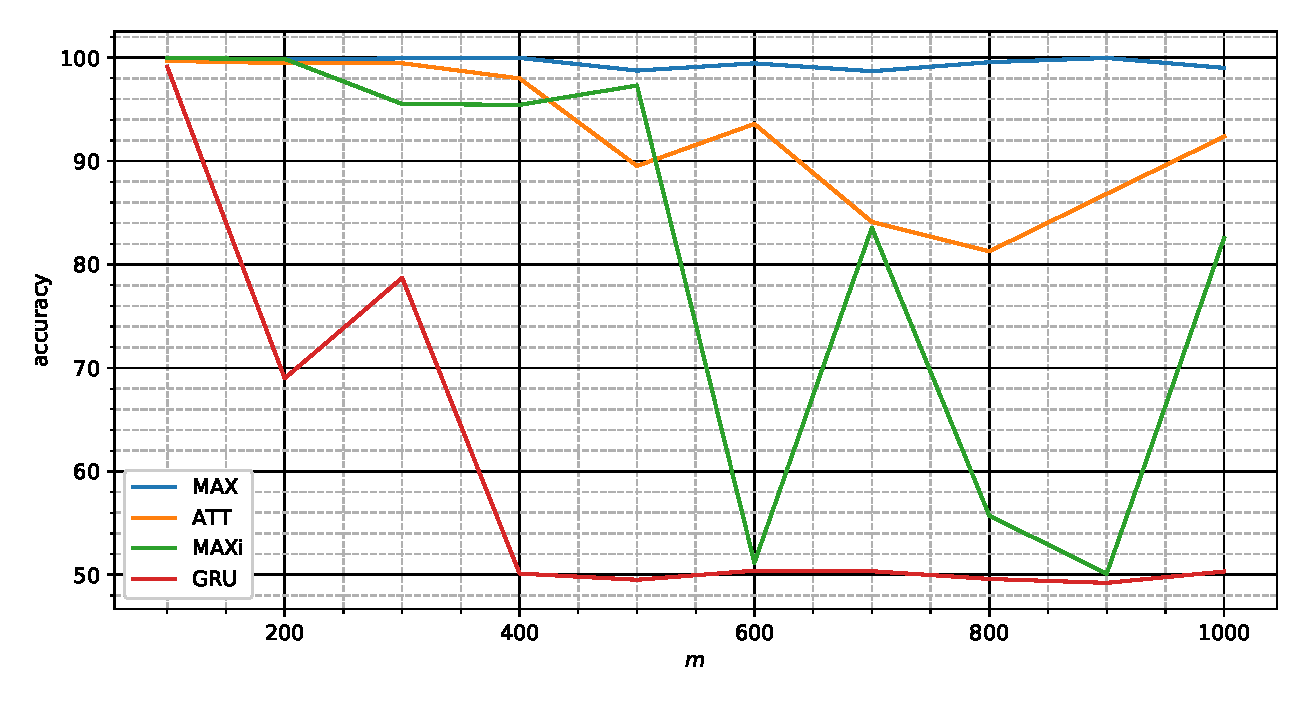
\includegraphics[width=0.7\textwidth]{imgMax/maxBaseDiff.eps}    
  \footnotesize
  \begin{tabular}{|p{\floatwidth}|}
    \hline
    \attvisB{0}{5}{0} \attvisB{9}{6}{0} \attvisB{2}{7}{0} \attvisB{1}{7}{0} \attvisB{8}{5}{0} \attvisB{4}{5}{0} \attvisB{2}{5}{0} \attvisB{8}{5}{0} \attvisB{9}{6}{0} \attvisB{1}{6}{0} \attvisB{4}{5}{0} \attvisB{6}{5}{0} \attvisB{8}{6}{0} \attvisB{8}{5}{0} \attvisB{6}{4}{0} \attvisB{6}{5}{0} \attvisB{8}{6}{0} \attvisB{7}{7}{0} \attvisB{3}{5}{0} \attvisB{0}{5}{0} \attvisB{2}{5}{0} \attvisB{5}{5}{0} \attvisB{9}{7}{0} \attvisB{7}{7}{0} \attvisB{9}{6}{0} \attvisB{5}{5}{0} \attvisB{8}{5}{0} \attvisB{2}{5}{0} \attvisB{4}{6}{0} \attvisB{9}{6}{0} \attvisB{5}{5}{0} \attvisB{5}{5}{0} \attvisB{6}{5}{0} \attvisB{5}{6}{0} \attvisB{1}{7}{0} \attvisB{7}{7}{0} \attvisB{6}{5}{0} \attvisB{3}{5}{0} \attvisB{2}{6}{0} \attvisB{2}{5}{0} \attvisB{2}{7}{0} \attvisB{1}{6}{100} \attvisB{3}{5}{100} \attvisB{1}{100}{100} \attvisB{2}{5}{0} \attvisB{5}{5}{0} \attvisB{0}{5}{0} \attvisB{8}{5}{0} \attvisB{9}{6}{0} \attvisB{5}{5}{0} \attvisB{4}{6}{0} \attvisB{0}{5}{0} \attvisB{3}{5}{0} \attvisB{2}{5}{0} \attvisB{3}{5}{0} \attvisB{0}{5}{0} \attvisB{6}{4}{0} \attvisB{0}{5}{0} \attvisB{0}{5}{0} \attvisB{8}{5}{0} \attvisB{6}{5}{0} \attvisB{7}{7}{0} \attvisB{9}{7}{0} \attvisB{1}{6}{0} \attvisB{6}{5}{0} \attvisB{4}{6}{0} \attvisB{0}{5}{0} \attvisB{5}{5}{0} \attvisB{7}{7}{0} \attvisB{0}{5}{0} \attvisB{6}{4}{0} \attvisB{4}{6}{0} \attvisB{6}{5}{0} \attvisB{0}{6}{0} \attvisB{6}{5}{0} \attvisB{1}{6}{0} \attvisB{5}{4}{0} \attvisB{4}{6}{0} \attvisB{3}{5}{0} \attvisB{2}{6}{0} \attvisB{5}{5}{0} \attvisB{2}{5}{0} \attvisB{6}{5}{0} \attvisB{7}{7}{0} \attvisB{4}{5}{0} \attvisB{2}{5}{0} \attvisB{5}{5}{0} \attvisB{2}{5}{0} \attvisB{5}{5}{0} \attvisB{8}{5}{0} \attvisB{9}{6}{0} \attvisB{9}{6}{0} \attvisB{5}{6}{0} \attvisB{7}{7}{0} \attvisB{6}{4}{0} \attvisB{5}{5}{0} \attvisB{4}{5}{0} \attvisB{2}{6}{0} \attvisB{7}{7}{0} \attvisB{9}{6}{0}
\\
    \hline
    \attvisB{5}{0}{0} \attvisB{3}{0}{0} \attvisB{6}{0}{0} \attvisB{9}{0}{0} \attvisB{0}{0}{0} \attvisB{9}{0}{0} \attvisB{1}{0}{0} \attvisB{8}{0}{0} \attvisB{0}{0}{0} \attvisB{1}{0}{0} \attvisB{5}{0}{0} \attvisB{4}{0}{0} \attvisB{5}{0}{0} \attvisB{0}{0}{0} \attvisB{4}{0}{0} \attvisB{7}{0}{0} \attvisB{1}{0}{0} \attvisB{6}{0}{0} \attvisB{2}{0}{0} \attvisB{3}{0}{0} \attvisB{2}{0}{0} \attvisB{9}{0}{0} \attvisB{2}{0}{0} \attvisB{6}{0}{0} \attvisB{8}{0}{0} \attvisB{8}{0}{0} \attvisB{2}{0}{0} \attvisB{6}{0}{0} \attvisB{1}{0}{0} \attvisB{1}{0}{0} \attvisB{2}{0}{0} \attvisB{3}{0}{0} \attvisB{6}{0}{0} \attvisB{3}{0}{0} \attvisB{6}{0}{0} \attvisB{4}{0}{0} \attvisB{4}{0}{0} \attvisB{6}{0}{0} \attvisB{6}{0}{0} \attvisB{8}{0}{0} \attvisB{9}{0}{0} \attvisB{9}{0}{0} \attvisB{3}{0}{0} \attvisB{5}{0}{0} \attvisB{6}{0}{0} \attvisB{4}{0}{0} \attvisB{2}{0}{0} \attvisB{4}{0}{0} \attvisB{7}{0}{0} \attvisB{0}{0}{0} \attvisB{3}{0}{0} \attvisB{3}{0}{0} \attvisB{8}{0}{0} \attvisB{5}{0}{0} \attvisB{5}{0}{0} \attvisB{4}{0}{0} \attvisB{6}{0}{0} \attvisB{9}{0}{0} \attvisB{2}{0}{0} \attvisB{3}{0}{0} \attvisB{2}{0}{0} \attvisB{9}{0}{0} \attvisB{5}{0}{0} \attvisB{5}{0}{0} \attvisB{3}{0}{0} \attvisB{5}{0}{0} \attvisB{7}{0}{0} \attvisB{8}{0}{0} \attvisB{0}{0}{0} \attvisB{4}{0}{0} \attvisB{7}{0}{0} \attvisB{1}{0}{0} \attvisB{3}{0}{0} \attvisB{6}{0}{0} \attvisB{6}{0}{0} \attvisB{3}{0}{0} \attvisB{8}{0}{0} \attvisB{8}{0}{0} \attvisB{8}{0}{0} \attvisB{8}{0}{0} \attvisB{6}{0}{0} \attvisB{9}{0}{0} \attvisB{6}{0}{0} \attvisB{0}{0}{0} \attvisB{6}{0}{0} \attvisB{4}{0}{100} \attvisB{0}{0}{100} \attvisB{1}{0}{100} \attvisB{5}{8}{0} \attvisB{4}{8}{0} \attvisB{9}{8}{0} \attvisB{5}{8}{0} \attvisB{5}{8}{0} \attvisB{5}{8}{0} \attvisB{9}{8}{0} \attvisB{7}{8}{0} \attvisB{6}{8}{0} \attvisB{5}{8}{0} \attvisB{8}{8}{0} \attvisB{4}{8}{0}

\\
    \hline
  \end{tabular}
\end{center}
\end{frame}


\subsection{Attention VS max, hierarchical VS plain}

\begin{frame}{Attention VS max, hierarchical VS plain}
  \begin{block}{Answered questions}
  \begin{itemize}
  \item[Q1] Implement \alert{large scale} study on deep learning
    applied to pathology reports
  \item[Q2] Apply \alert{novel} deep learning techniques, like
    \alert{attention} models and \alert{acs{bert}}
  \item[Q4] \alert{Compare} novel \alert{attention}-based and
    \alert{hierarchical} techniques with simpler models
  \item[Q6] \alert{Investigate} the possibility to give
    \alert{interpretation} to deep learning models
  \end{itemize}
\end{block}
\begin{itemize}
\item \alert{Temporal} setting
\item On \alert{main site} and \alert{type} tasks
\item Different \alert{difficulty} classes
\end{itemize}
\end{frame}

\begin{frame}{Attention VS max, hierarchical VS plain}
  \small
  \begin{center}
    \begin{tabular}{ccccc}
    \hline
    \textbf{SITE}&Accuracy&Top 3 Acc.&Top 5 Acc.&MacroF1\\
    \hline
    \svm{}     &89.7&95.9&96.8&60.0\\
    \xgb{}     &89.1&95.8&97.2&58.0\\
    \hline
    \gru{}     &89.9&96.5&97.7&58.3\\
    \bert{}    &89.9&96.3&97.8&56.6\\
    \hline
    \maxi{}    &88.0&95.4&96.2&46.1\\
    \maxh{}    &89.9&96.2&97.8&58.8\\
    \softmaxh{}&89.9&96.3&97.7&58.0\\
    \maxp{}    &\textbf{90.3}&\textbf{96.6}&\textbf{98.1}&\textbf{61.9}\\
    \softmax{} &90.1&96.2&97.6&60.0\\
    \hline
    \end{tabular}
        \tiny
    \begin{tabular}{cccc|ccc}
    \hline
    &\multicolumn{3}{c}{Topography}&\multicolumn{3}{c}{Morphology}\\
        &easy&avg.&hard&easy&avg.&hard\\
        &($1000<s$)&($100<s\leq 1000$)&($s\leq 100$)&($1000<s$)&($100<s\leq 1000$)&($s\leq 100$)\\
    &(4 cls)&(18 cls)&(39 cls)&(5 cls)&(18 cls)&(111 cls)\\
    \hline
    \svm{}     &95.7&\textbf{86.9}&50.9&90.5&68.6&48.4\\
    \xgb{}     &95.6&86.4&48.2&92.0&72.4&54.8\\
    \hline
    \gru{}     &\textbf{96.1}&72.2&48.0&91.4&71.6&49.7\\
    \bert{}    &95.7&73.2&44.9&\textbf{92.9}&\textbf{74.4}&43.9\\    
    \hline
    \maxi{}    &95.0&66.6&31.4&87.1&41.9&25.1\\
    \maxh{}    &95.8&72.4&48.8&92.7&71.8&48.8\\
    \softmaxh{}&96.0&73.1&47.1&91.9&72.3&52.6\\
    \maxp{}    &96.0&73.3&\textbf{53.1}&92.7&72.3&53.8\\
    \softmax{} &96.0&73.1&50.3&92.8&72.3&\textbf{56.7}\\
    \hline
  \end{tabular}

  \end{center}
\end{frame}

\begin{frame}{Interpretability}
  \centering
  \tiny
    \begin{tabular}{|c|c|c|}
    \hline
    $y_i$&\textrm{Relevant} $\vect{h}_{i,j}$&$x_{i,j}$\textrm{, relevant} $\vect{h}_{i,j}$\\
    \hline
    61&\begin{minipage}{\attTableIcdoWidth}\att{61}{red}{100} \att{(PROSTATE}{red}{100} \att{GLAND)}{red}{100} \end{minipage}&\begin{minipage}{\attTableTextWidth}\att{DISOMOGENICITA}{red}{0} \att{'}{red}{0} \att{DIFFUSE}{red}{0} \att{.}{red}{0} \att{PSA}{red}{85} \att{NON}{red}{0} \att{PERVENUTO}{red}{0} \att{.}{red}{0} \att{ADENOCARCINOMA}{red}{0} \att{PROSTATICO}{red}{100} \att{A}{red}{0} \att{GRADO}{red}{1} \att{DI}{red}{0} \att{DIFFERENZIAZIONE}{red}{0} \att{MEDIO}{red}{0} \att{-}{red}{0} \att{BASSO}{red}{0} \att{(}{red}{0} \att{GLEASON}{red}{100} \att{3}{red}{4} \att{+}{red}{0} \att{4}{red}{0} \att{)}{red}{0} \att{NEI}{red}{0} \att{PRELIEVI}{red}{0} \att{DI}{red}{0} \att{CUI}{red}{0} \att{AI}{red}{0} \att{NN}{red}{0} \att{.}{red}{0} \att{2}{red}{0} \att{E}{red}{0} \att{3}{red}{0} \att{.}{red}{0} \att{AGOBIOPSIA}{red}{0} \att{DELLA}{red}{0} \att{PROSTATA}{red}{100} \att{:}{red}{0} \att{1}{red}{0} \att{)}{red}{0} \att{1}{red}{0} \att{PRELIEVO}{red}{0} \att{LL}{red}{0} \att{DX}{red}{0} \att{.}{red}{0} \att{2}{red}{0} \att{)}{red}{0} \att{2}{red}{0} \att{PRELIEVI}{red}{0} \att{ML}{red}{0} \att{DX}{red}{0} \att{.}{red}{0} \att{3}{red}{0} \att{)}{red}{0} \att{2}{red}{0} \att{PRELIEVI}{red}{0} \att{M}{red}{0} \att{DX}{red}{0} \att{.}{red}{0} \att{4}{red}{0} \att{)}{red}{0} \att{1}{red}{0} \att{PRELIEVO}{red}{0} \att{M}{red}{0} \att{SX}{red}{0} \att{.}{red}{0} \att{5}{red}{0} \att{)}{red}{0} \att{2}{red}{0} \att{PRELIEVI}{red}{0} \att{ML}{red}{0} \att{SX}{red}{0} \att{.}{red}{0} \att{6}{red}{0} \att{)}{red}{0} \att{1}{red}{0} \att{PRELIEVO}{red}{0} \att{LL}{red}{0} \att{SX}{red}{0} \att{.}{red}{0} \att{7}{red}{0} \att{)}{red}{0} \att{1}{red}{0} \att{PRELIEVO}{red}{0} \att{TRANSIZIONALE}{red}{54} \att{SX}{red}{1} \att{.}{red}{0} \att{8}{red}{0} \att{)}{red}{0} \att{1}{red}{0} \att{PRELIEVO}{red}{0} \att{TRANSIZIONALE}{red}{19} \att{DX}{red}{7} \att{.}{red}{0} \end{minipage}\\ % doc valid 49


    \hline
    20&\begin{minipage}{\attTableIcdoWidth}\att{\att{\att{18}{red}{100}}{green}{0}}{blue}{0} \att{\att{\att{(COLON)}{red}{100}}{green}{0}}{blue}{0} \\\\\att{\att{\att{20}{red}{0}}{green}{100}}{blue}{0} \att{\att{\att{(RECTUM)}{red}{0}}{green}{100}}{blue}{0} \\\\\att{\att{\att{21}{red}{0}}{green}{0}}{blue}{100} \att{\att{\att{(ANUS}{red}{0}}{green}{0}}{blue}{100} \att{\att{\att{AND}{red}{0}}{green}{0}}{blue}{100} \att{\att{\att{ANAL}{red}{0}}{green}{0}}{blue}{100} \att{\att{\att{CANAL)}{red}{0}}{green}{0}}{blue}{100} \end{minipage}&\begin{minipage}{\attTableTextWidth}\att{\att{\att{ISOLATI}{red}{0}}{green}{0}}{blue}{0} \att{\att{\att{FRAMMENTI}{red}{0}}{green}{0}}{blue}{0} \att{\att{\att{RIFERIBILI}{red}{0}}{green}{0}}{blue}{0} \att{\att{\att{AD}{red}{0}}{green}{0}}{blue}{0} \att{\att{\att{ADENOMA}{red}{0}}{green}{0}}{blue}{0} \att{\att{\att{TUBULARE}{red}{100}}{green}{0}}{blue}{0} \att{\att{\att{INTESTINALE}{red}{100}}{green}{1}}{blue}{0} \att{\att{\att{DI}{red}{2}}{green}{0}}{blue}{0} \att{\att{\att{ALTO}{red}{4}}{green}{0}}{blue}{0} \att{\att{\att{GRADO}{red}{1}}{green}{0}}{blue}{0} \att{\att{\att{.}{red}{0}}{green}{0}}{blue}{0} \att{\att{\att{FRAMMENTI}{red}{0}}{green}{0}}{blue}{0} \att{\att{\att{(}{red}{0}}{green}{0}}{blue}{0} \att{\att{\att{NR}{red}{0}}{green}{0}}{blue}{0} \att{\att{\att{.}{red}{0}}{green}{0}}{blue}{0} \att{\att{\att{2}{red}{0}}{green}{0}}{blue}{0} \att{\att{\att{)}{red}{0}}{green}{0}}{blue}{0} \att{\att{\att{DI}{red}{0}}{green}{0}}{blue}{0} \att{\att{\att{POLIPO}{red}{88}}{green}{63}}{blue}{0} \att{\att{\att{PEDUNCOLATO}{red}{100}}{green}{0}}{blue}{0} \att{\att{\att{A}{red}{0}}{green}{0}}{blue}{0} \att{\att{\att{20}{red}{0}}{green}{0}}{blue}{0} \att{\att{\att{CM}{red}{0}}{green}{0}}{blue}{0} \att{\att{\att{DALL}{red}{61}}{green}{0}}{blue}{0} \att{\att{\att{'}{red}{0}}{green}{0}}{blue}{0} \att{\att{\att{ORIFIZIO}{red}{0}}{green}{96}}{blue}{89} \att{\att{\att{ANALE}{red}{0}}{green}{100}}{blue}{100} \att{\att{\att{.}{red}{0}}{green}{30}}{blue}{0} \att{\att{\att{(}{red}{0}}{green}{0}}{blue}{0} \att{\att{\att{ESEGUITA}{red}{0}}{green}{0}}{blue}{0} \att{\att{\att{COLORAZIONE}{red}{0}}{green}{0}}{blue}{0} \att{\att{\att{EMATOSSILINA}{red}{0}}{green}{0}}{blue}{0} \att{\att{\att{-}{red}{0}}{green}{0}}{blue}{0} \att{\att{\att{EOSINA}{red}{0}}{green}{0}}{blue}{0} \att{\att{\att{)}{red}{0}}{green}{0}}{blue}{0} \att{\att{\att{.}{red}{0}}{green}{0}}{blue}{0} \end{minipage}\\ % doc valid 2


    \hline
    %61&\begin{minipage}{\attTableIcdoWidth}\att{61}{red}{100} \att{(PROSTATE}{red}{100} \att{GLAND)}{red}{100} \end{minipage}&\begin{minipage}{\attTableTextWidth}\att{DISOMOGENICITA}{red}{0} \att{'}{red}{0} \att{DIFFUSE}{red}{0} \att{.}{red}{0} \att{PSA}{red}{85} \att{NON}{red}{0} \att{PERVENUTO}{red}{0} \att{.}{red}{0} \att{ADENOCARCINOMA}{red}{0} \att{PROSTATICO}{red}{100} \att{A}{red}{0} \att{GRADO}{red}{1} \att{DI}{red}{0} \att{DIFFERENZIAZIONE}{red}{0} \att{MEDIO}{red}{0} \att{-}{red}{0} \att{BASSO}{red}{0} \att{(}{red}{0} \att{GLEASON}{red}{100} \att{3}{red}{4} \att{+}{red}{0} \att{4}{red}{0} \att{)}{red}{0} \att{NEI}{red}{0} \att{PRELIEVI}{red}{0} \att{DI}{red}{0} \att{CUI}{red}{0} \att{AI}{red}{0} \att{NN}{red}{0} \att{.}{red}{0} \att{2}{red}{0} \att{E}{red}{0} \att{3}{red}{0} \att{.}{red}{0} \att{AGOBIOPSIA}{red}{0} \att{DELLA}{red}{0} \att{PROSTATA}{red}{100} \att{:}{red}{0} \att{1}{red}{0} \att{)}{red}{0} \att{1}{red}{0} \att{PRELIEVO}{red}{0} \att{LL}{red}{0} \att{DX}{red}{0} \att{.}{red}{0} \att{2}{red}{0} \att{)}{red}{0} \att{2}{red}{0} \att{PRELIEVI}{red}{0} \att{ML}{red}{0} \att{DX}{red}{0} \att{.}{red}{0} \att{3}{red}{0} \att{)}{red}{0} \att{2}{red}{0} \att{PRELIEVI}{red}{0} \att{M}{red}{0} \att{DX}{red}{0} \att{.}{red}{0} \att{4}{red}{0} \att{)}{red}{0} \att{1}{red}{0} \att{PRELIEVO}{red}{0} \att{M}{red}{0} \att{SX}{red}{0} \att{.}{red}{0} \att{5}{red}{0} \att{)}{red}{0} \att{2}{red}{0} \att{PRELIEVI}{red}{0} \att{ML}{red}{0} \att{SX}{red}{0} \att{.}{red}{0} \att{6}{red}{0} \att{)}{red}{0} \att{1}{red}{0} \att{PRELIEVO}{red}{0} \att{LL}{red}{0} \att{SX}{red}{0} \att{.}{red}{0} \att{7}{red}{0} \att{)}{red}{0} \att{1}{red}{0} \att{PRELIEVO}{red}{0} \att{TRANSIZIONALE}{red}{54} \att{SX}{red}{1} \att{.}{red}{0} \att{8}{red}{0} \att{)}{red}{0} \att{1}{red}{0} \att{PRELIEVO}{red}{0} \att{TRANSIZIONALE}{red}{19} \att{DX}{red}{7} \att{.}{red}{0} \end{minipage}\\ % doc valid 49


    %\hline
    34&\begin{minipage}{\attTableIcdoWidth}\att{\att{\att{\att{34}{red}{100}}{green}{0}}{blue}{0}}{black}{0} \att{\att{\att{\att{(BRONCHUS}{red}{100}}{green}{0}}{blue}{0}}{black}{0} \att{\att{\att{\att{AND}{red}{100}}{green}{0}}{blue}{0}}{black}{0} \att{\att{\att{\att{LUNG)}{red}{100}}{green}{0}}{blue}{0}}{black}{0} \\\\\att{\att{\att{\att{56}{red}{0}}{green}{100}}{blue}{0}}{black}{0} \att{\att{\att{\att{(OVARY)}{red}{0}}{green}{100}}{blue}{0}}{black}{0} \\\\\att{\att{\att{\att{67}{red}{0}}{green}{0}}{blue}{100}}{black}{0} \att{\att{\att{\att{(BLADDER)}{red}{0}}{green}{0}}{blue}{100}}{black}{0} \\\\\att{\att{\att{\att{80}{red}{0}}{green}{0}}{blue}{0}}{black}{100} \att{\att{\att{\att{(UNKNOWN}{red}{0}}{green}{0}}{blue}{0}}{black}{100} \att{\att{\att{\att{PRIMARY}{red}{0}}{green}{0}}{blue}{0}}{black}{100} \att{\att{\att{\att{SITE)}{red}{0}}{green}{0}}{blue}{0}}{black}{100} \end{minipage}&\begin{minipage}{\attTableTextWidth}\att{\att{\att{\att{VERSAMENTO}{red}{5}}{green}{0}}{blue}{0}}{black}{0} \att{\att{\att{\att{PLEURICO}{red}{100}}{green}{55}}{blue}{0}}{black}{5} \att{\att{\att{\att{SX}{red}{24}}{green}{0}}{blue}{0}}{black}{0} \att{\att{\att{\att{DI}{red}{0}}{green}{0}}{blue}{0}}{black}{0} \att{\att{\att{\att{N}{red}{0}}{green}{0}}{blue}{0}}{black}{0} \att{\att{\att{\att{.}{red}{0}}{green}{0}}{blue}{0}}{black}{0} \att{\att{\att{\att{D}{red}{0}}{green}{0}}{blue}{0}}{black}{0} \att{\att{\att{\att{.}{red}{0}}{green}{0}}{blue}{0}}{black}{0} \att{\att{\att{\att{D}{red}{0}}{green}{0}}{blue}{0}}{black}{0} \att{\att{\att{\att{.}{red}{0}}{green}{0}}{blue}{0}}{black}{0} \att{\att{\att{\att{E}{red}{0}}{green}{0}}{blue}{0}}{black}{0} \att{\att{\att{\att{ADDENSAMENTI}{red}{16}}{green}{0}}{blue}{0}}{black}{0} \att{\att{\att{\att{POLMONARI}{red}{100}}{green}{0}}{blue}{0}}{black}{0} \att{\att{\att{\att{DI}{red}{0}}{green}{0}}{blue}{0}}{black}{0} \att{\att{\att{\att{N}{red}{0}}{green}{0}}{blue}{0}}{black}{0} \att{\att{\att{\att{.}{red}{0}}{green}{0}}{blue}{0}}{black}{0} \att{\att{\att{\att{D}{red}{0}}{green}{0}}{blue}{0}}{black}{0} \att{\att{\att{\att{.}{red}{0}}{green}{0}}{blue}{0}}{black}{0} \att{\att{\att{\att{D}{red}{0}}{green}{0}}{blue}{0}}{black}{0} \att{\att{\att{\att{.}{red}{0}}{green}{0}}{blue}{0}}{black}{0} \att{\att{\att{\att{,}{red}{0}}{green}{0}}{blue}{0}}{black}{0} \att{\att{\att{\att{NODULI}{red}{0}}{green}{0}}{blue}{0}}{black}{0} \att{\att{\att{\att{PARETE}{red}{0}}{green}{0}}{blue}{28}}{black}{0} \att{\att{\att{\att{ADDOMINALE}{red}{1}}{green}{0}}{blue}{0}}{black}{0} \att{\att{\att{\att{.}{red}{0}}{green}{0}}{blue}{0}}{black}{0} \att{\att{\att{\att{INFILTRAZIONE}{red}{0}}{green}{0}}{blue}{0}}{black}{0} \att{\att{\att{\att{CANCERIGNA}{red}{100}}{green}{0}}{blue}{0}}{black}{13} \att{\att{\att{\att{DEGLI}{red}{100}}{green}{0}}{blue}{0}}{black}{83} \att{\att{\att{\att{STROMI}{red}{7}}{green}{0}}{blue}{0}}{black}{100} \att{\att{\att{\att{CONNETTIVO}{red}{0}}{green}{0}}{blue}{0}}{black}{0} \att{\att{\att{\att{-}{red}{1}}{green}{0}}{blue}{0}}{black}{0} \att{\att{\att{\att{ADIPOSI}{red}{0}}{green}{0}}{blue}{0}}{black}{78} \att{\att{\att{\att{.}{red}{30}}{green}{0}}{blue}{0}}{black}{1} \att{\att{\att{\att{IMMUNOISTOCHIMICA}{red}{100}}{green}{0}}{blue}{0}}{black}{95} \att{\att{\att{\att{:}{red}{17}}{green}{0}}{blue}{0}}{black}{98} \att{\att{\att{\att{CK7}{red}{100}}{green}{0}}{blue}{0}}{black}{100} \att{\att{\att{\att{+}{red}{99}}{green}{0}}{blue}{0}}{black}{0} \att{\att{\att{\att{,}{red}{77}}{green}{0}}{blue}{0}}{black}{51} \att{\att{\att{\att{CK20}{red}{100}}{green}{0}}{blue}{0}}{black}{100} \att{\att{\att{\att{-}{red}{100}}{green}{0}}{blue}{0}}{black}{1} \att{\att{\att{\att{,}{red}{84}}{green}{0}}{blue}{0}}{black}{37} \att{\att{\att{\att{TTF}{red}{100}}{green}{0}}{blue}{0}}{black}{100} \att{\att{\att{\att{-}{red}{100}}{green}{0}}{blue}{0}}{black}{0} \att{\att{\att{\att{1}{red}{3}}{green}{0}}{blue}{0}}{black}{0} \att{\att{\att{\att{-}{red}{31}}{green}{0}}{blue}{0}}{black}{0} \att{\att{\att{\att{,}{red}{69}}{green}{0}}{blue}{0}}{black}{0} \att{\att{\att{\att{PROTEINA}{red}{99}}{green}{0}}{blue}{0}}{black}{70} \att{\att{\att{\att{S}{red}{0}}{green}{0}}{blue}{0}}{black}{4} \att{\att{\att{\att{-}{red}{0}}{green}{0}}{blue}{0}}{black}{0} \att{\att{\att{\att{100}{red}{2}}{green}{0}}{blue}{0}}{black}{1} \att{\att{\att{\att{-}{red}{0}}{green}{0}}{blue}{0}}{black}{0} \att{\att{\att{\att{.}{red}{0}}{green}{0}}{blue}{0}}{black}{0} \att{\att{\att{\att{LESIONE}{red}{0}}{green}{0}}{blue}{0}}{black}{0} \att{\att{\att{\att{DI}{red}{0}}{green}{0}}{blue}{0}}{black}{0} \att{\att{\att{\att{CM}{red}{0}}{green}{0}}{blue}{0}}{black}{0} \att{\att{\att{\att{2}{red}{1}}{green}{0}}{blue}{0}}{black}{0} \att{\att{\att{\att{,}{red}{0}}{green}{0}}{blue}{0}}{black}{0} \att{\att{\att{\att{0}{red}{28}}{green}{0}}{blue}{0}}{black}{0} \att{\att{\att{\att{X}{red}{0}}{green}{0}}{blue}{0}}{black}{0} \att{\att{\att{\att{1}{red}{0}}{green}{0}}{blue}{0}}{black}{0} \att{\att{\att{\att{,}{red}{1}}{green}{0}}{blue}{0}}{black}{0} \att{\att{\att{\att{3}{red}{0}}{green}{0}}{blue}{0}}{black}{0} \att{\att{\att{\att{X}{red}{0}}{green}{0}}{blue}{0}}{black}{0} \att{\att{\att{\att{0}{red}{2}}{green}{0}}{blue}{0}}{black}{0} \att{\att{\att{\att{,}{red}{7}}{green}{0}}{blue}{0}}{black}{0} \att{\att{\att{\att{7}{red}{0}}{green}{0}}{blue}{0}}{black}{0} \att{\att{\att{\att{.}{red}{0}}{green}{0}}{blue}{0}}{black}{0} \att{\att{\att{\att{1}{red}{3}}{green}{0}}{blue}{0}}{black}{0} \att{\att{\att{\att{-}{red}{3}}{green}{0}}{blue}{0}}{black}{0} \att{\att{\att{\att{2}{red}{0}}{green}{0}}{blue}{0}}{black}{0} \att{\att{\att{\att{)}{red}{0}}{green}{0}}{blue}{0}}{black}{0} \att{\att{\att{\att{SEZIONI}{red}{23}}{green}{0}}{blue}{0}}{black}{0} \att{\att{\att{\att{SERIATE}{red}{87}}{green}{0}}{blue}{0}}{black}{3} \att{\att{\att{\att{.}{red}{65}}{green}{0}}{blue}{0}}{black}{0} \end{minipage}\\ % doc valid 923


    \hline
  \end{tabular}
\end{frame}

\begin{frame}{Interpretability}
  \begin{figure}
  \centering
  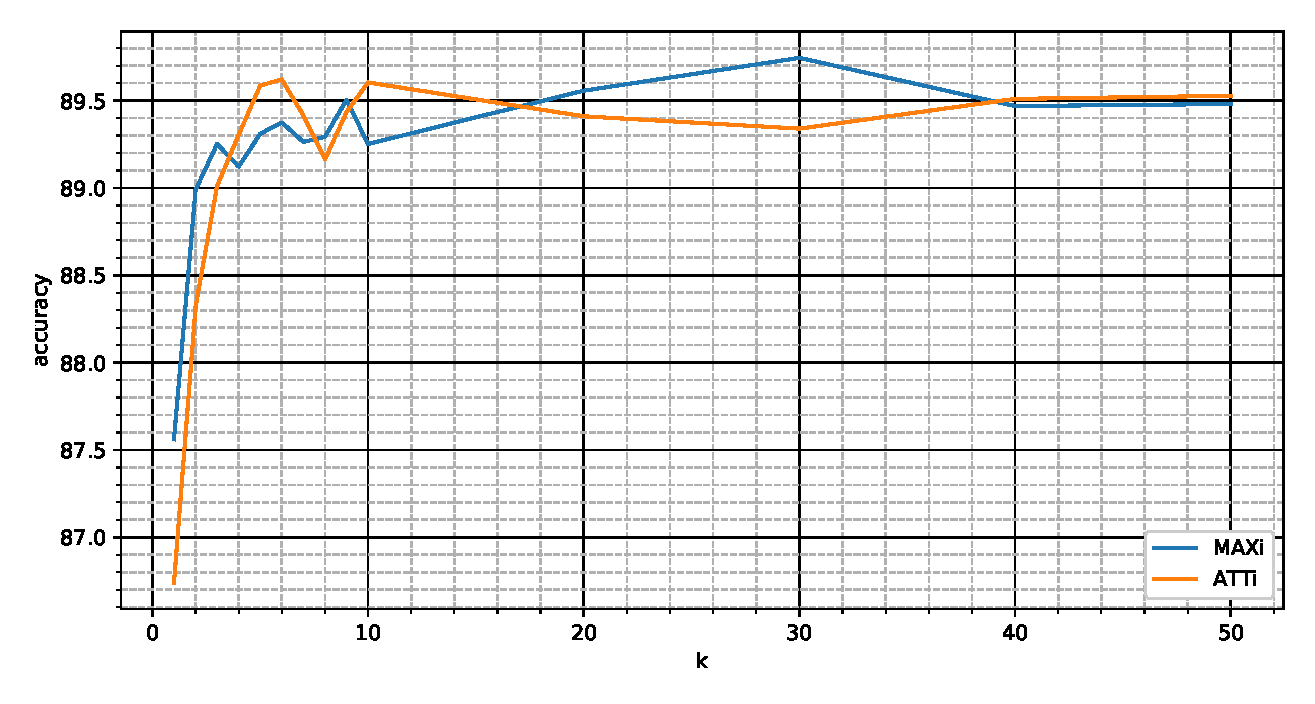
\includegraphics[width=\textwidth]{img/plotSintex.eps}
  \caption{Training of a plain \ac{gru} model on a dataset created
    using \maxi{} and \softmaxi{} to keep the first $k$ words}
\end{figure}
\end{frame}

\begin{frame}
  \begin{center}
    \textbf{\calligra\Huge The End.}\\
    
\includegraphics[width=5cm]{img/ornament.eps}\\[1cm]
    {\huge\calligra Questions? Thank you!}
  \end{center}
\end{frame}

\section{Conclusions}


%\appendix
\backupbegin

\begin{frame}[allowframebreaks]{Bibliography}
  \scriptsize
  %\nocite{*}
  \bibliography{slides}
\end{frame}


\backupend

\end{document}

%%% Local Variables:
%%% mode: latex
%%% TeX-master: t
%%% End:
